\documentclass[tikz,10pt,border=.1mm]{standalone}
\usepackage{mathpazo,gnuplot-lua-tikz,siunitx,pgfplots,xcolor,structmech,mathtools}
\usepackage{amsmath,amsfonts,amssymb,siunitx,float,subcaption,setspace,booktabs,diagbox,bm,tikz,structmech,mathtools,tikz-3dplot,pgfplots,gnuplot-lua-tikz,url}
\usetikzlibrary{decorations.pathmorphing,shapes.geometric}
\pgfplotsset{compat=1.16}
\newcommand*{\mb}[1]{\bm{#1}}
\newcommand*{\mT}{\mathrm{T}}
\newcommand*{\md}[1]{\mathrm{d}#1}
\newcommand*{\eqsref}[1]{Eq.~(\ref{#1})}
\newcommand*{\figref}[1]{Fig.~\ref{#1}}
\newcommand*{\tabref}[1]{Table~\ref{#1}}
\newcommand*{\algoref}[1]{Algorithm~\ref{#1}}
\newcommand*{\secref}[1]{\S~\ref{#1}}
\newcommand*{\diag}[1]{\text{diag}\left(#1\right)}
\newcommand*{\sign}[1]{\text{sign}\left(#1\right)}
\newcommand*{\dev}[1]{\text{dev}\left(#1\right)}
\newcommand*{\tr}[1]{\text{trace}\left(#1\right)}
\newcommand*{\ddfrac}[2]{\dfrac{\md{#1}}{\md{#2}}}
\newcommand*{\pdfrac}[2]{\dfrac{\partial{#1}}{\partial{#2}}}
\newcommand{\bsigma}{\mb{\sigma}}
\newcommand{\bvarepsilon}{\mb{\varepsilon}}
\newcommand{\beeta}{\mb{\eta}}
\newcommand{\bn}{\mb{n}}
\newcommand{\balpha}{\mb{\alpha}}
\newcommand{\bbeta}{\mb{\beta}}
\newcommand{\bgamma}{\mb{\gamma}}
\newcommand{\bq}{\mb{q}}
\newcommand{\bs}{\mb{s}}
\newcommand{\bc}{\mb{c}}
\newcommand{\be}{\mb{e}}
\newcommand{\bv}{\mb{v}}
\begin{document}\scriptsize
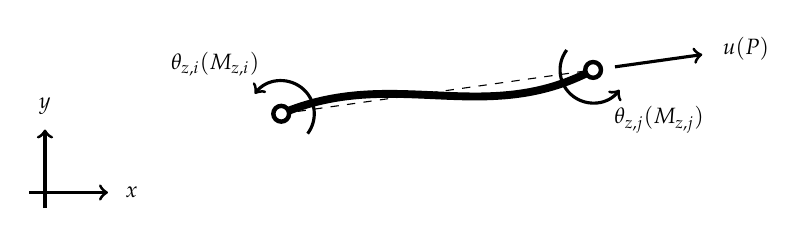
\begin{tikzpicture}
\CoorOrigin{-3,-1}
\begin{scope}[rotate=8]
\setstructmech{convention=direction}
\draw[line width=1mm](0,0)to[in=200,out=15](4,0);
\draw[dashed](0,0)--(4,0);
\node[ultra thick]at(0,0)[circle,draw,inner sep=0,minimum size=2mm,fill=white]{};
\node[ultra thick]at(4,0)[circle,draw,inner sep=0,minimum size=2mm,fill=white]{};
\NodalForce{0,0}[N][N][\theta_{z,i}(M_{z,i})][1.4];
\NodalForce{4,0}[-u(P)][N][\theta_{z,j}(M_{z,j})]{180}[1.4];
\end{scope}
\end{tikzpicture}
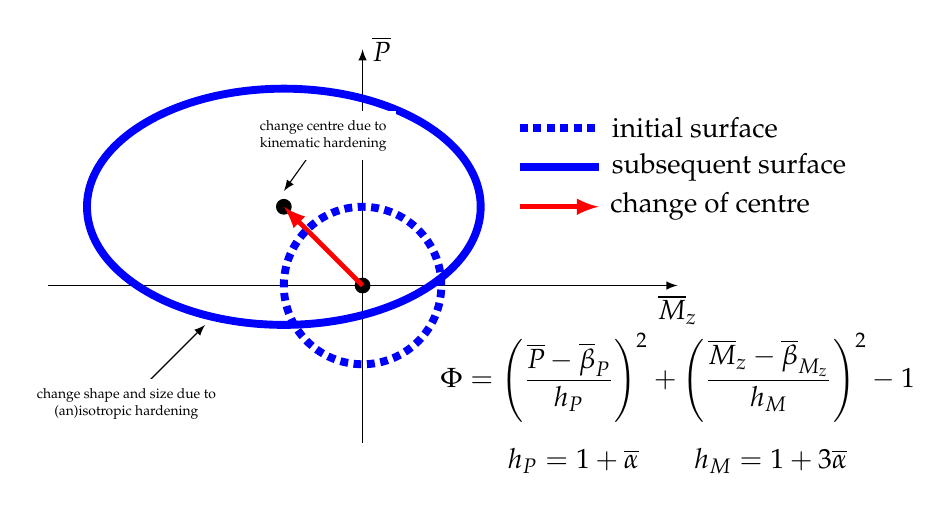
\begin{tikzpicture}[>=latex]
\draw[->](-4,0)--(4,0)node[below]{$\overline{M}_z$};
\draw[->](0,-2)--(0,3)node[right]{$\overline{P}$};
\coordinate(A)at(0,0);
\coordinate(B)at(-1,1);
\node[fill=black,circle,inner sep=0,minimum size=2mm]at(A){};
\node[fill=black,circle,inner sep=0,minimum size=2mm]at(B){};
\draw[->,draw=red,line width=.6mm](A)--(B);
\node[dotted,circle,draw=blue,line width=1mm,minimum width=2cm,minimum height=2cm]at(A){};
\node[ellipse,draw=blue,line width=1mm,minimum width=5cm,minimum height=3cm](e)at(B){};
\node[align=center]at(4,-1.5){$\Phi=\left(\dfrac{\overline{P}-\overline{\beta}_P}{h_P}\right)^2+\left(\dfrac{\overline{M}_z-\overline{\beta}_{M_z}}{h_M}\right)^2-1$\\[3mm]$h_P=1+\overline{\alpha}\qquad{}h_M=1+3\overline{\alpha}$};
\draw[dotted,draw=blue,line width=1mm](2,2)--++(1,0)node[right]{initial surface};
\draw[draw=blue,line width=1mm](2,1.5)--++(1,0)node[right,align=left]{subsequent surface};
\draw[->,draw=red,line width=.6mm](2,1)--++(1,0)node[right]{change of centre};
\draw[<-](-2,-.5)--++(-1,-1)node[fill=white,align=center,font=\tiny]{change shape and size due to\\(an)isotropic hardening};
\draw[<-](B)++(0,.2)--++(.5,.7)node[fill=white,align=center,font=\tiny]{change centre due to\\kinematic hardening};
\end{tikzpicture}
\begin{tikzpicture}[]
\begin{axis}[
view={65}{10},
axis lines=center,
axis equal image,
axis on top,
y dir=reverse,
xmin=0,ymin=0,zmin=0,
xmax=.5,ymax=.6,zmax=.4,
xticklabel=\empty,
yticklabel=\empty,
zticklabel=\empty,
xlabel=$\overline{\mb{e}}^p_{M_{z,j}}$,
ylabel=$\overline{\mb{e}}^p_{M_{z,i}}$,
zlabel=$\overline{\mb{e}}^p_{P}$,
every axis y label/.append style={at=(ticklabel* cs:0)}]
\addplot3[smooth,line width=.4mm,red,dotted]file{PIC/XZ.txt};
\addplot3[smooth,line width=.4mm,blue,dashed]file{PIC/YZ.txt};
\addplot3[smooth,line width=.8mm]file{PIC/XYZ.txt};
\end{axis}
\draw[line width=.4mm,blue,dashed](8,2)--++(.5,0)node[right=2mm]{$\overline{\alpha}_i$ history};
\draw[line width=.4mm,red,dotted](8,1.5)--++(.5,0)node[right=2mm]{$\overline{\alpha}_j$ history};
\draw[line width=.8mm](8,.7)--++(.5,0)node[right=2mm,align=left]{$\overline{\alpha}$ history characterises\\the length of path};
\end{tikzpicture}

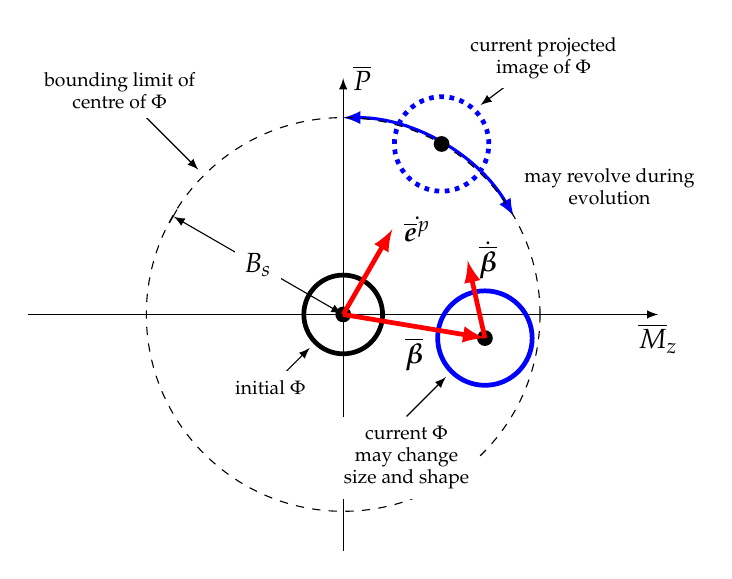
\begin{tikzpicture}[>=latex]
\draw[->](-4,0)--(4,0)node[below]{$\overline{M}_z$};
\draw[->](0,-3)--(0,3)node[right]{$\overline{P}$};
\coordinate(A)at(0,0);
\coordinate(B)at(1.8,-.3);
\coordinate(C)at(60:2.5);
\draw[<->,line width=.4mm,draw=blue]($(A)+(30:2.5)$)node[above right,font=\scriptsize,align=center]{may revolve during\\evolution}arc(30:90:2.5);
\draw[|<->|](A)--++(150:2.5)node[midway,fill=white]{$B_s$};
\node[fill=black,circle,inner sep=0,minimum size=2mm]at(A){};
\node[fill=black,circle,inner sep=0,minimum size=2mm]at(B){};
\node[fill=black,circle,inner sep=0,minimum size=2mm]at(C){};
\node[dashed,circle,draw=black,minimum width=5cm,minimum height=5cm]at(A){};
\node[circle,draw,line width=.6mm,minimum width=1cm,minimum height=1cm]at(A){};
\node[circle,draw=blue,line width=.6mm,minimum width=1.2cm,minimum height=1.2cm]at(B){};
\node[dotted,circle,draw=blue,line width=.6mm,minimum width=1.2cm,minimum height=1.2cm]at(C){};
\draw[->,draw=red,line width=.6mm](A)--(B)node[midway,below]{$\overline{\bbeta}$};
\draw[->,draw=red,line width=.6mm](B)--($(B)!.4!(C)$)node[right]{$\dot{\overline{\bbeta}}$};
\draw[->,draw=red,line width=.6mm](A)--($(A)!.5!(C)$)node[right]{$\dot{\mb{\overline{e}}^p}$};
\draw[<-](135:2.6)--++(-1,1)node[fill=white,align=center,font=\scriptsize]{bounding limit of\\centre of $\Phi$};
\draw[<-]($(B)+(-135:.7)$)--++(-.5,-.5)node[anchor=north,fill=white,align=center,font=\scriptsize]{current $\Phi$\\may change\\size and shape};
\draw[<-]($(A)+(-135:.6)$)--++(-.5,-.5)node[fill=white,align=center,font=\scriptsize]{initial $\Phi$};
\draw[<-]($(C)+(45:.7)$)--++(.8,.6)node[fill=white,align=center,font=\scriptsize]{current projected\\image of $\Phi$};
\end{tikzpicture}
\begin{tikzpicture}[gnuplot]
%% generated with GNUPLOT 5.4p3 (Lua 5.4; terminal rev. Jun 2020, script rev. 115)
%% 07/08/2022 00:53:32
\path (0.000,0.000) rectangle (12.000,4.000);
\gpcolor{color=gp lt color axes}
\gpsetlinetype{gp lt axes}
\gpsetdashtype{gp dt axes}
\gpsetlinewidth{0.50}
\draw[gp path] (0.120,0.560)--(5.999,0.560);
\gpcolor{color=gp lt color border}
\gpsetlinetype{gp lt border}
\gpsetdashtype{gp dt solid}
\gpsetlinewidth{1.00}
\draw[gp path] (0.120,0.560)--(0.300,0.560);
\draw[gp path] (5.999,0.560)--(5.819,0.560);
\node[gp node right] at (-0.064,0.560) {$-2$};
\gpcolor{color=gp lt color axes}
\gpsetlinetype{gp lt axes}
\gpsetdashtype{gp dt axes}
\gpsetlinewidth{0.50}
\draw[gp path] (0.120,1.280)--(5.999,1.280);
\gpcolor{color=gp lt color border}
\gpsetlinetype{gp lt border}
\gpsetdashtype{gp dt solid}
\gpsetlinewidth{1.00}
\draw[gp path] (0.120,1.280)--(0.300,1.280);
\draw[gp path] (5.999,1.280)--(5.819,1.280);
\node[gp node right] at (-0.064,1.280) {$-1$};
\gpcolor{color=gp lt color axes}
\gpsetlinetype{gp lt axes}
\gpsetdashtype{gp dt axes}
\gpsetlinewidth{0.50}
\draw[gp path] (0.120,2.000)--(5.999,2.000);
\gpcolor{color=gp lt color border}
\gpsetlinetype{gp lt border}
\gpsetdashtype{gp dt solid}
\gpsetlinewidth{1.00}
\draw[gp path] (0.120,2.000)--(0.300,2.000);
\draw[gp path] (5.999,2.000)--(5.819,2.000);
\node[gp node right] at (-0.064,2.000) {$0$};
\gpcolor{color=gp lt color axes}
\gpsetlinetype{gp lt axes}
\gpsetdashtype{gp dt axes}
\gpsetlinewidth{0.50}
\draw[gp path] (0.120,2.719)--(5.999,2.719);
\gpcolor{color=gp lt color border}
\gpsetlinetype{gp lt border}
\gpsetdashtype{gp dt solid}
\gpsetlinewidth{1.00}
\draw[gp path] (0.120,2.719)--(0.300,2.719);
\draw[gp path] (5.999,2.719)--(5.819,2.719);
\node[gp node right] at (-0.064,2.719) {$1$};
\gpcolor{color=gp lt color axes}
\gpsetlinetype{gp lt axes}
\gpsetdashtype{gp dt axes}
\gpsetlinewidth{0.50}
\draw[gp path] (0.120,3.439)--(5.999,3.439);
\gpcolor{color=gp lt color border}
\gpsetlinetype{gp lt border}
\gpsetdashtype{gp dt solid}
\gpsetlinewidth{1.00}
\draw[gp path] (0.120,3.439)--(0.300,3.439);
\draw[gp path] (5.999,3.439)--(5.819,3.439);
\node[gp node right] at (-0.064,3.439) {$2$};
\gpcolor{color=gp lt color axes}
\gpsetlinetype{gp lt axes}
\gpsetdashtype{gp dt axes}
\gpsetlinewidth{0.50}
\draw[gp path] (0.447,0.200)--(0.447,0.380)--(0.447,3.799);
\gpcolor{color=gp lt color border}
\gpsetlinetype{gp lt border}
\gpsetdashtype{gp dt solid}
\gpsetlinewidth{1.00}
\draw[gp path] (0.447,0.200)--(0.447,0.380);
\draw[gp path] (0.447,3.799)--(0.447,3.619);
\node[gp node center] at (0.447,-0.108) {$-4$};
\gpcolor{color=gp lt color axes}
\gpsetlinetype{gp lt axes}
\gpsetdashtype{gp dt axes}
\gpsetlinewidth{0.50}
\draw[gp path] (1.100,0.200)--(1.100,3.799);
\gpcolor{color=gp lt color border}
\gpsetlinetype{gp lt border}
\gpsetdashtype{gp dt solid}
\gpsetlinewidth{1.00}
\draw[gp path] (1.100,0.200)--(1.100,0.380);
\draw[gp path] (1.100,3.799)--(1.100,3.619);
\node[gp node center] at (1.100,-0.108) {$-3$};
\gpcolor{color=gp lt color axes}
\gpsetlinetype{gp lt axes}
\gpsetdashtype{gp dt axes}
\gpsetlinewidth{0.50}
\draw[gp path] (1.753,0.200)--(1.753,3.799);
\gpcolor{color=gp lt color border}
\gpsetlinetype{gp lt border}
\gpsetdashtype{gp dt solid}
\gpsetlinewidth{1.00}
\draw[gp path] (1.753,0.200)--(1.753,0.380);
\draw[gp path] (1.753,3.799)--(1.753,3.619);
\node[gp node center] at (1.753,-0.108) {$-2$};
\gpcolor{color=gp lt color axes}
\gpsetlinetype{gp lt axes}
\gpsetdashtype{gp dt axes}
\gpsetlinewidth{0.50}
\draw[gp path] (2.406,0.200)--(2.406,3.799);
\gpcolor{color=gp lt color border}
\gpsetlinetype{gp lt border}
\gpsetdashtype{gp dt solid}
\gpsetlinewidth{1.00}
\draw[gp path] (2.406,0.200)--(2.406,0.380);
\draw[gp path] (2.406,3.799)--(2.406,3.619);
\node[gp node center] at (2.406,-0.108) {$-1$};
\gpcolor{color=gp lt color axes}
\gpsetlinetype{gp lt axes}
\gpsetdashtype{gp dt axes}
\gpsetlinewidth{0.50}
\draw[gp path] (3.060,0.200)--(3.060,3.799);
\gpcolor{color=gp lt color border}
\gpsetlinetype{gp lt border}
\gpsetdashtype{gp dt solid}
\gpsetlinewidth{1.00}
\draw[gp path] (3.060,0.200)--(3.060,0.380);
\draw[gp path] (3.060,3.799)--(3.060,3.619);
\node[gp node center] at (3.060,-0.108) {$0$};
\gpcolor{color=gp lt color axes}
\gpsetlinetype{gp lt axes}
\gpsetdashtype{gp dt axes}
\gpsetlinewidth{0.50}
\draw[gp path] (3.713,0.200)--(3.713,3.799);
\gpcolor{color=gp lt color border}
\gpsetlinetype{gp lt border}
\gpsetdashtype{gp dt solid}
\gpsetlinewidth{1.00}
\draw[gp path] (3.713,0.200)--(3.713,0.380);
\draw[gp path] (3.713,3.799)--(3.713,3.619);
\node[gp node center] at (3.713,-0.108) {$1$};
\gpcolor{color=gp lt color axes}
\gpsetlinetype{gp lt axes}
\gpsetdashtype{gp dt axes}
\gpsetlinewidth{0.50}
\draw[gp path] (4.366,0.200)--(4.366,3.799);
\gpcolor{color=gp lt color border}
\gpsetlinetype{gp lt border}
\gpsetdashtype{gp dt solid}
\gpsetlinewidth{1.00}
\draw[gp path] (4.366,0.200)--(4.366,0.380);
\draw[gp path] (4.366,3.799)--(4.366,3.619);
\node[gp node center] at (4.366,-0.108) {$2$};
\gpcolor{color=gp lt color axes}
\gpsetlinetype{gp lt axes}
\gpsetdashtype{gp dt axes}
\gpsetlinewidth{0.50}
\draw[gp path] (5.019,0.200)--(5.019,3.799);
\gpcolor{color=gp lt color border}
\gpsetlinetype{gp lt border}
\gpsetdashtype{gp dt solid}
\gpsetlinewidth{1.00}
\draw[gp path] (5.019,0.200)--(5.019,0.380);
\draw[gp path] (5.019,3.799)--(5.019,3.619);
\node[gp node center] at (5.019,-0.108) {$3$};
\gpcolor{color=gp lt color axes}
\gpsetlinetype{gp lt axes}
\gpsetdashtype{gp dt axes}
\gpsetlinewidth{0.50}
\draw[gp path] (5.672,0.200)--(5.672,3.799);
\gpcolor{color=gp lt color border}
\gpsetlinetype{gp lt border}
\gpsetdashtype{gp dt solid}
\gpsetlinewidth{1.00}
\draw[gp path] (5.672,0.200)--(5.672,0.380);
\draw[gp path] (5.672,3.799)--(5.672,3.619);
\node[gp node center] at (5.672,-0.108) {$4$};
\draw[gp path] (0.120,3.799)--(0.120,0.200)--(5.999,0.200)--(5.999,3.799)--cycle;
\node[gp node center,rotate=-270] at (-0.724,1.999) {resistance};
\node[gp node center] at (3.059,-0.569) {deformation};
\gpcolor{rgb color={0.894,0.102,0.110}}
\gpsetlinewidth{2.00}
\draw[gp path] (3.060,2.000)--(3.125,2.071)--(3.190,2.143)--(3.255,2.215)--(3.321,2.287)%
  --(3.386,2.359)--(3.451,2.431)--(3.517,2.503)--(3.582,2.575)--(3.647,2.647)--(3.713,2.719)%
  --(3.778,2.726)--(3.843,2.732)--(3.909,2.739)--(3.974,2.745)--(4.039,2.752)--(4.105,2.759)%
  --(4.170,2.765)--(4.235,2.772)--(4.301,2.778)--(4.366,2.785)--(4.301,2.713)--(4.235,2.641)%
  --(4.170,2.569)--(4.105,2.497)--(4.039,2.425)--(3.974,2.353)--(3.909,2.281)--(3.843,2.209)%
  --(3.778,2.137)--(3.713,2.065)--(3.647,1.993)--(3.582,1.921)--(3.517,1.849)--(3.451,1.777)%
  --(3.386,1.705)--(3.321,1.633)--(3.255,1.561)--(3.190,1.489)--(3.125,1.417)--(3.060,1.345)%
  --(2.994,1.273)--(2.929,1.213)--(2.864,1.207)--(2.798,1.200)--(2.733,1.193)--(2.668,1.187)%
  --(2.602,1.180)--(2.537,1.174)--(2.472,1.167)--(2.406,1.161)--(2.341,1.154)--(2.276,1.148)%
  --(2.210,1.141)--(2.145,1.135)--(2.080,1.128)--(2.014,1.121)--(1.949,1.115)--(1.884,1.108)%
  --(1.818,1.102)--(1.753,1.095)--(1.818,1.167)--(1.884,1.239)--(1.949,1.311)--(2.014,1.383)%
  --(2.080,1.455)--(2.145,1.527)--(2.210,1.599)--(2.276,1.671)--(2.341,1.743)--(2.406,1.815)%
  --(2.472,1.887)--(2.537,1.959)--(2.602,2.031)--(2.668,2.103)--(2.733,2.175)--(2.798,2.247)%
  --(2.864,2.319)--(2.929,2.391)--(2.994,2.463)--(3.060,2.535)--(3.125,2.607)--(3.190,2.679)%
  --(3.255,2.751)--(3.321,2.823)--(3.386,2.895)--(3.451,2.909)--(3.517,2.916)--(3.582,2.923)%
  --(3.647,2.929)--(3.713,2.936)--(3.778,2.942)--(3.843,2.949)--(3.909,2.955)--(3.974,2.962)%
  --(4.039,2.968)--(4.105,2.975)--(4.170,2.981)--(4.235,2.988)--(4.301,2.995)--(4.366,3.001)%
  --(4.431,3.008)--(4.497,3.014)--(4.562,3.021)--(4.627,3.027)--(4.693,3.034)--(4.758,3.040)%
  --(4.823,3.047)--(4.889,3.053)--(4.954,3.060)--(5.019,3.066)--(4.954,2.995)--(4.889,2.923)%
  --(4.823,2.851)--(4.758,2.779)--(4.693,2.707)--(4.627,2.635)--(4.562,2.563)--(4.497,2.491)%
  --(4.431,2.419)--(4.366,2.347)--(4.301,2.275)--(4.235,2.203)--(4.170,2.131)--(4.105,2.059)%
  --(4.039,1.987)--(3.974,1.915)--(3.909,1.843)--(3.843,1.771)--(3.778,1.699)--(3.713,1.627)%
  --(3.647,1.555)--(3.582,1.483)--(3.517,1.411)--(3.451,1.339)--(3.386,1.267)--(3.321,1.195)%
  --(3.255,1.123)--(3.190,1.051)--(3.125,0.979)--(3.060,0.930)--(2.994,0.924)--(2.929,0.917)%
  --(2.864,0.911)--(2.798,0.904)--(2.733,0.897)--(2.668,0.891)--(2.602,0.884)--(2.537,0.878)%
  --(2.472,0.871)--(2.406,0.865)--(2.341,0.858)--(2.276,0.852)--(2.210,0.845)--(2.145,0.839)%
  --(2.080,0.832)--(2.014,0.825)--(1.949,0.819)--(1.884,0.812)--(1.818,0.806)--(1.753,0.799)%
  --(1.688,0.793)--(1.622,0.786)--(1.557,0.780)--(1.492,0.773)--(1.426,0.767)--(1.361,0.760)%
  --(1.296,0.754)--(1.230,0.747)--(1.165,0.740)--(1.100,0.734)--(1.165,0.806)--(1.230,0.878)%
  --(1.296,0.950)--(1.361,1.022)--(1.426,1.094)--(1.492,1.166)--(1.557,1.238)--(1.622,1.310)%
  --(1.688,1.382)--(1.753,1.454)--(1.818,1.526)--(1.884,1.598)--(1.949,1.670)--(2.014,1.742)%
  --(2.080,1.814)--(2.145,1.886)--(2.210,1.958)--(2.276,2.030)--(2.341,2.102)--(2.406,2.173)%
  --(2.472,2.245)--(2.537,2.317)--(2.602,2.389)--(2.668,2.461)--(2.733,2.533)--(2.798,2.605)%
  --(2.864,2.677)--(2.929,2.749)--(2.994,2.821)--(3.060,2.893)--(3.125,2.965)--(3.190,3.037)%
  --(3.255,3.109)--(3.321,3.181)--(3.386,3.253)--(3.451,3.271)--(3.517,3.277)--(3.582,3.284)%
  --(3.647,3.290)--(3.713,3.297)--(3.778,3.303)--(3.843,3.310)--(3.909,3.316)--(3.974,3.323)%
  --(4.039,3.329)--(4.105,3.336)--(4.170,3.343)--(4.235,3.349)--(4.301,3.356)--(4.366,3.362)%
  --(4.431,3.369)--(4.497,3.375)--(4.562,3.382)--(4.627,3.388)--(4.693,3.395)--(4.758,3.401)%
  --(4.823,3.408)--(4.889,3.415)--(4.954,3.421)--(5.019,3.428)--(5.084,3.434)--(5.150,3.441)%
  --(5.215,3.447)--(5.280,3.454)--(5.346,3.460)--(5.411,3.467)--(5.476,3.473)--(5.542,3.480)%
  --(5.607,3.487)--(5.672,3.493)--(5.607,3.421)--(5.542,3.349)--(5.476,3.277)--(5.411,3.205)%
  --(5.346,3.133)--(5.280,3.061)--(5.215,2.989)--(5.150,2.917)--(5.084,2.845)--(5.019,2.773)%
  --(4.954,2.701)--(4.889,2.629)--(4.823,2.557)--(4.758,2.485)--(4.693,2.413)--(4.627,2.341)%
  --(4.562,2.269)--(4.497,2.197)--(4.431,2.125)--(4.366,2.053)--(4.301,1.981)--(4.235,1.909)%
  --(4.170,1.838)--(4.105,1.766)--(4.039,1.694)--(3.974,1.622)--(3.909,1.550)--(3.843,1.478)%
  --(3.778,1.406)--(3.713,1.334)--(3.647,1.262)--(3.582,1.190)--(3.517,1.118)--(3.451,1.046)%
  --(3.386,0.974)--(3.321,0.902)--(3.255,0.830)--(3.190,0.758)--(3.125,0.686)--(3.060,0.614)%
  --(2.994,0.542)--(2.929,0.503)--(2.864,0.496)--(2.798,0.490)--(2.733,0.483)--(2.668,0.476)%
  --(2.602,0.470)--(2.537,0.463)--(2.472,0.457)--(2.406,0.450)--(2.341,0.444)--(2.276,0.437)%
  --(2.210,0.431)--(2.145,0.424)--(2.080,0.418)--(2.014,0.411)--(1.949,0.405)--(1.884,0.398)%
  --(1.818,0.391)--(1.753,0.385)--(1.688,0.378)--(1.622,0.372)--(1.557,0.365)--(1.492,0.359)%
  --(1.426,0.352)--(1.361,0.346)--(1.296,0.339)--(1.230,0.333)--(1.165,0.326)--(1.100,0.319)%
  --(1.035,0.313)--(0.969,0.306)--(0.904,0.300)--(0.839,0.293)--(0.773,0.287)--(0.708,0.280)%
  --(0.643,0.274)--(0.577,0.267)--(0.512,0.261)--(0.447,0.254)--(0.512,0.326)--(0.577,0.398)%
  --(0.643,0.470)--(0.708,0.542)--(0.773,0.614)--(0.839,0.686)--(0.904,0.758)--(0.969,0.830)%
  --(1.035,0.902)--(1.100,0.974)--(1.165,1.046)--(1.230,1.118)--(1.296,1.190)--(1.361,1.262)%
  --(1.426,1.334)--(1.492,1.406)--(1.557,1.478)--(1.622,1.550)--(1.688,1.622)--(1.753,1.694)%
  --(1.818,1.766)--(1.884,1.838)--(1.949,1.910)--(2.014,1.982)--(2.080,2.054)--(2.145,2.125)%
  --(2.210,2.197)--(2.276,2.269)--(2.341,2.341)--(2.406,2.413)--(2.472,2.485)--(2.537,2.557)%
  --(2.602,2.629)--(2.668,2.701)--(2.733,2.773)--(2.798,2.845)--(2.864,2.917)--(2.929,2.989)%
  --(2.994,3.061)--(3.060,3.133);
\gpcolor{color=gp lt color border}
\gpsetlinewidth{1.00}
\draw[gp path] (0.120,3.799)--(0.120,0.200)--(5.999,0.200)--(5.999,3.799)--cycle;
%% coordinates of the plot area
\gpdefrectangularnode{gp plot 1}{\pgfpoint{0.120cm}{0.200cm}}{\pgfpoint{5.999cm}{3.799cm}}
\gpcolor{color=gp lt color axes}
\gpsetlinetype{gp lt axes}
\gpsetdashtype{gp dt axes}
\gpsetlinewidth{0.50}
\draw[gp path] (6.327,0.200)--(6.327,3.799);
\gpcolor{color=gp lt color border}
\gpsetlinetype{gp lt border}
\gpsetdashtype{gp dt solid}
\gpsetlinewidth{1.00}
\draw[gp path] (6.327,0.200)--(6.327,0.380);
\draw[gp path] (6.327,3.799)--(6.327,3.619);
\node[gp node center] at (6.327,-0.108) {$-4$};
\gpcolor{color=gp lt color axes}
\gpsetlinetype{gp lt axes}
\gpsetdashtype{gp dt axes}
\gpsetlinewidth{0.50}
\draw[gp path] (6.980,0.200)--(6.980,3.799);
\gpcolor{color=gp lt color border}
\gpsetlinetype{gp lt border}
\gpsetdashtype{gp dt solid}
\gpsetlinewidth{1.00}
\draw[gp path] (6.980,0.200)--(6.980,0.380);
\draw[gp path] (6.980,3.799)--(6.980,3.619);
\node[gp node center] at (6.980,-0.108) {$-3$};
\gpcolor{color=gp lt color axes}
\gpsetlinetype{gp lt axes}
\gpsetdashtype{gp dt axes}
\gpsetlinewidth{0.50}
\draw[gp path] (7.633,0.200)--(7.633,3.799);
\gpcolor{color=gp lt color border}
\gpsetlinetype{gp lt border}
\gpsetdashtype{gp dt solid}
\gpsetlinewidth{1.00}
\draw[gp path] (7.633,0.200)--(7.633,0.380);
\draw[gp path] (7.633,3.799)--(7.633,3.619);
\node[gp node center] at (7.633,-0.108) {$-2$};
\gpcolor{color=gp lt color axes}
\gpsetlinetype{gp lt axes}
\gpsetdashtype{gp dt axes}
\gpsetlinewidth{0.50}
\draw[gp path] (8.286,0.200)--(8.286,3.799);
\gpcolor{color=gp lt color border}
\gpsetlinetype{gp lt border}
\gpsetdashtype{gp dt solid}
\gpsetlinewidth{1.00}
\draw[gp path] (8.286,0.200)--(8.286,0.380);
\draw[gp path] (8.286,3.799)--(8.286,3.619);
\node[gp node center] at (8.286,-0.108) {$-1$};
\gpcolor{color=gp lt color axes}
\gpsetlinetype{gp lt axes}
\gpsetdashtype{gp dt axes}
\gpsetlinewidth{0.50}
\draw[gp path] (8.940,0.200)--(8.940,3.799);
\gpcolor{color=gp lt color border}
\gpsetlinetype{gp lt border}
\gpsetdashtype{gp dt solid}
\gpsetlinewidth{1.00}
\draw[gp path] (8.940,0.200)--(8.940,0.380);
\draw[gp path] (8.940,3.799)--(8.940,3.619);
\node[gp node center] at (8.940,-0.108) {$0$};
\gpcolor{color=gp lt color axes}
\gpsetlinetype{gp lt axes}
\gpsetdashtype{gp dt axes}
\gpsetlinewidth{0.50}
\draw[gp path] (9.593,0.200)--(9.593,3.799);
\gpcolor{color=gp lt color border}
\gpsetlinetype{gp lt border}
\gpsetdashtype{gp dt solid}
\gpsetlinewidth{1.00}
\draw[gp path] (9.593,0.200)--(9.593,0.380);
\draw[gp path] (9.593,3.799)--(9.593,3.619);
\node[gp node center] at (9.593,-0.108) {$1$};
\gpcolor{color=gp lt color axes}
\gpsetlinetype{gp lt axes}
\gpsetdashtype{gp dt axes}
\gpsetlinewidth{0.50}
\draw[gp path] (10.246,0.200)--(10.246,3.799);
\gpcolor{color=gp lt color border}
\gpsetlinetype{gp lt border}
\gpsetdashtype{gp dt solid}
\gpsetlinewidth{1.00}
\draw[gp path] (10.246,0.200)--(10.246,0.380);
\draw[gp path] (10.246,3.799)--(10.246,3.619);
\node[gp node center] at (10.246,-0.108) {$2$};
\gpcolor{color=gp lt color axes}
\gpsetlinetype{gp lt axes}
\gpsetdashtype{gp dt axes}
\gpsetlinewidth{0.50}
\draw[gp path] (10.899,0.200)--(10.899,3.799);
\gpcolor{color=gp lt color border}
\gpsetlinetype{gp lt border}
\gpsetdashtype{gp dt solid}
\gpsetlinewidth{1.00}
\draw[gp path] (10.899,0.200)--(10.899,0.380);
\draw[gp path] (10.899,3.799)--(10.899,3.619);
\node[gp node center] at (10.899,-0.108) {$3$};
\gpcolor{color=gp lt color axes}
\gpsetlinetype{gp lt axes}
\gpsetdashtype{gp dt axes}
\gpsetlinewidth{0.50}
\draw[gp path] (11.552,0.200)--(11.552,0.380)--(11.552,3.799);
\gpcolor{color=gp lt color border}
\gpsetlinetype{gp lt border}
\gpsetdashtype{gp dt solid}
\gpsetlinewidth{1.00}
\draw[gp path] (11.552,0.200)--(11.552,0.380);
\draw[gp path] (11.552,3.799)--(11.552,3.619);
\node[gp node center] at (11.552,-0.108) {$4$};
\draw[gp path] (11.879,0.666)--(11.699,0.666);
\node[gp node left] at (12.063,0.666) {$0.091$};
\draw[gp path] (11.879,1.546)--(11.699,1.546);
\node[gp node left] at (12.063,1.546) {$0.2$};
\draw[gp path] (11.879,2.571)--(11.699,2.571);
\node[gp node left] at (12.063,2.571) {$0.5$};
\draw[gp path] (11.879,3.346)--(11.699,3.346);
\node[gp node left] at (12.063,3.346) {$1$};
\draw[gp path] (6.000,3.799)--(6.000,0.200)--(11.879,0.200)--(11.879,3.799)--cycle;
\node[gp node center,rotate=-270] at (13.321,1.999) {stiffness};
\node[gp node center] at (8.939,-0.569) {deformation};
\gpcolor{rgb color={0.216,0.494,0.722}}
\gpsetpointsize{4.00}
\gp3point{gp mark 7}{}{(8.940,3.346)}
\gp3point{gp mark 7}{}{(9.005,3.346)}
\gp3point{gp mark 7}{}{(9.070,3.346)}
\gp3point{gp mark 7}{}{(9.135,3.346)}
\gp3point{gp mark 7}{}{(9.201,3.346)}
\gp3point{gp mark 7}{}{(9.266,3.346)}
\gp3point{gp mark 7}{}{(9.331,3.346)}
\gp3point{gp mark 7}{}{(9.397,3.346)}
\gp3point{gp mark 7}{}{(9.462,3.346)}
\gp3point{gp mark 7}{}{(9.527,3.346)}
\gp3point{gp mark 7}{}{(9.593,3.346)}
\gp3point{gp mark 7}{}{(9.658,0.665)}
\gp3point{gp mark 7}{}{(9.723,0.665)}
\gp3point{gp mark 7}{}{(9.789,0.665)}
\gp3point{gp mark 7}{}{(9.854,0.665)}
\gp3point{gp mark 7}{}{(9.919,0.665)}
\gp3point{gp mark 7}{}{(9.985,0.665)}
\gp3point{gp mark 7}{}{(10.050,0.665)}
\gp3point{gp mark 7}{}{(10.115,0.665)}
\gp3point{gp mark 7}{}{(10.181,0.665)}
\gp3point{gp mark 7}{}{(10.246,0.665)}
\gp3point{gp mark 7}{}{(10.181,3.346)}
\gp3point{gp mark 7}{}{(10.115,3.346)}
\gp3point{gp mark 7}{}{(10.050,3.346)}
\gp3point{gp mark 7}{}{(9.985,3.346)}
\gp3point{gp mark 7}{}{(9.919,3.346)}
\gp3point{gp mark 7}{}{(9.854,3.346)}
\gp3point{gp mark 7}{}{(9.789,3.346)}
\gp3point{gp mark 7}{}{(9.723,3.346)}
\gp3point{gp mark 7}{}{(9.658,3.346)}
\gp3point{gp mark 7}{}{(9.593,3.346)}
\gp3point{gp mark 7}{}{(9.527,3.346)}
\gp3point{gp mark 7}{}{(9.462,3.346)}
\gp3point{gp mark 7}{}{(9.397,3.346)}
\gp3point{gp mark 7}{}{(9.331,3.346)}
\gp3point{gp mark 7}{}{(9.266,3.346)}
\gp3point{gp mark 7}{}{(9.201,3.346)}
\gp3point{gp mark 7}{}{(9.135,3.346)}
\gp3point{gp mark 7}{}{(9.070,3.346)}
\gp3point{gp mark 7}{}{(9.005,3.346)}
\gp3point{gp mark 7}{}{(8.940,3.346)}
\gp3point{gp mark 7}{}{(8.874,3.346)}
\gp3point{gp mark 7}{}{(8.809,3.144)}
\gp3point{gp mark 7}{}{(8.744,0.665)}
\gp3point{gp mark 7}{}{(8.678,0.665)}
\gp3point{gp mark 7}{}{(8.613,0.665)}
\gp3point{gp mark 7}{}{(8.548,0.665)}
\gp3point{gp mark 7}{}{(8.482,0.665)}
\gp3point{gp mark 7}{}{(8.417,0.665)}
\gp3point{gp mark 7}{}{(8.352,0.665)}
\gp3point{gp mark 7}{}{(8.286,0.665)}
\gp3point{gp mark 7}{}{(8.221,0.665)}
\gp3point{gp mark 7}{}{(8.156,0.665)}
\gp3point{gp mark 7}{}{(8.090,0.665)}
\gp3point{gp mark 7}{}{(8.025,0.665)}
\gp3point{gp mark 7}{}{(7.960,0.665)}
\gp3point{gp mark 7}{}{(7.894,0.665)}
\gp3point{gp mark 7}{}{(7.829,0.665)}
\gp3point{gp mark 7}{}{(7.764,0.665)}
\gp3point{gp mark 7}{}{(7.698,0.665)}
\gp3point{gp mark 7}{}{(7.633,0.665)}
\gp3point{gp mark 7}{}{(7.698,3.346)}
\gp3point{gp mark 7}{}{(7.764,3.346)}
\gp3point{gp mark 7}{}{(7.829,3.346)}
\gp3point{gp mark 7}{}{(7.894,3.346)}
\gp3point{gp mark 7}{}{(7.960,3.346)}
\gp3point{gp mark 7}{}{(8.025,3.346)}
\gp3point{gp mark 7}{}{(8.090,3.346)}
\gp3point{gp mark 7}{}{(8.156,3.346)}
\gp3point{gp mark 7}{}{(8.221,3.346)}
\gp3point{gp mark 7}{}{(8.286,3.346)}
\gp3point{gp mark 7}{}{(8.352,3.346)}
\gp3point{gp mark 7}{}{(8.417,3.346)}
\gp3point{gp mark 7}{}{(8.482,3.346)}
\gp3point{gp mark 7}{}{(8.548,3.346)}
\gp3point{gp mark 7}{}{(8.613,3.346)}
\gp3point{gp mark 7}{}{(8.678,3.346)}
\gp3point{gp mark 7}{}{(8.744,3.346)}
\gp3point{gp mark 7}{}{(8.809,3.346)}
\gp3point{gp mark 7}{}{(8.874,3.346)}
\gp3point{gp mark 7}{}{(8.940,3.346)}
\gp3point{gp mark 7}{}{(9.005,3.346)}
\gp3point{gp mark 7}{}{(9.070,3.346)}
\gp3point{gp mark 7}{}{(9.135,3.346)}
\gp3point{gp mark 7}{}{(9.201,3.346)}
\gp3point{gp mark 7}{}{(9.266,3.346)}
\gp3point{gp mark 7}{}{(9.331,1.566)}
\gp3point{gp mark 7}{}{(9.397,0.665)}
\gp3point{gp mark 7}{}{(9.462,0.665)}
\gp3point{gp mark 7}{}{(9.527,0.665)}
\gp3point{gp mark 7}{}{(9.593,0.665)}
\gp3point{gp mark 7}{}{(9.658,0.665)}
\gp3point{gp mark 7}{}{(9.723,0.665)}
\gp3point{gp mark 7}{}{(9.789,0.665)}
\gp3point{gp mark 7}{}{(9.854,0.665)}
\gp3point{gp mark 7}{}{(9.919,0.665)}
\gp3point{gp mark 7}{}{(9.985,0.665)}
\gp3point{gp mark 7}{}{(10.050,0.665)}
\gp3point{gp mark 7}{}{(10.115,0.665)}
\gp3point{gp mark 7}{}{(10.181,0.665)}
\gp3point{gp mark 7}{}{(10.246,0.665)}
\gp3point{gp mark 7}{}{(10.311,0.665)}
\gp3point{gp mark 7}{}{(10.377,0.665)}
\gp3point{gp mark 7}{}{(10.442,0.665)}
\gp3point{gp mark 7}{}{(10.507,0.665)}
\gp3point{gp mark 7}{}{(10.573,0.665)}
\gp3point{gp mark 7}{}{(10.638,0.665)}
\gp3point{gp mark 7}{}{(10.703,0.665)}
\gp3point{gp mark 7}{}{(10.769,0.665)}
\gp3point{gp mark 7}{}{(10.834,0.665)}
\gp3point{gp mark 7}{}{(10.899,0.665)}
\gp3point{gp mark 7}{}{(10.834,3.346)}
\gp3point{gp mark 7}{}{(10.769,3.346)}
\gp3point{gp mark 7}{}{(10.703,3.346)}
\gp3point{gp mark 7}{}{(10.638,3.346)}
\gp3point{gp mark 7}{}{(10.573,3.346)}
\gp3point{gp mark 7}{}{(10.507,3.346)}
\gp3point{gp mark 7}{}{(10.442,3.346)}
\gp3point{gp mark 7}{}{(10.377,3.346)}
\gp3point{gp mark 7}{}{(10.311,3.346)}
\gp3point{gp mark 7}{}{(10.246,3.346)}
\gp3point{gp mark 7}{}{(10.181,3.346)}
\gp3point{gp mark 7}{}{(10.115,3.346)}
\gp3point{gp mark 7}{}{(10.050,3.346)}
\gp3point{gp mark 7}{}{(9.985,3.346)}
\gp3point{gp mark 7}{}{(9.919,3.346)}
\gp3point{gp mark 7}{}{(9.854,3.346)}
\gp3point{gp mark 7}{}{(9.789,3.346)}
\gp3point{gp mark 7}{}{(9.723,3.346)}
\gp3point{gp mark 7}{}{(9.658,3.346)}
\gp3point{gp mark 7}{}{(9.593,3.346)}
\gp3point{gp mark 7}{}{(9.527,3.346)}
\gp3point{gp mark 7}{}{(9.462,3.346)}
\gp3point{gp mark 7}{}{(9.397,3.346)}
\gp3point{gp mark 7}{}{(9.331,3.346)}
\gp3point{gp mark 7}{}{(9.266,3.346)}
\gp3point{gp mark 7}{}{(9.201,3.346)}
\gp3point{gp mark 7}{}{(9.135,3.346)}
\gp3point{gp mark 7}{}{(9.070,3.346)}
\gp3point{gp mark 7}{}{(9.005,3.346)}
\gp3point{gp mark 7}{}{(8.940,2.913)}
\gp3point{gp mark 7}{}{(8.874,0.665)}
\gp3point{gp mark 7}{}{(8.809,0.665)}
\gp3point{gp mark 7}{}{(8.744,0.665)}
\gp3point{gp mark 7}{}{(8.678,0.665)}
\gp3point{gp mark 7}{}{(8.613,0.665)}
\gp3point{gp mark 7}{}{(8.548,0.665)}
\gp3point{gp mark 7}{}{(8.482,0.665)}
\gp3point{gp mark 7}{}{(8.417,0.665)}
\gp3point{gp mark 7}{}{(8.352,0.665)}
\gp3point{gp mark 7}{}{(8.286,0.665)}
\gp3point{gp mark 7}{}{(8.221,0.665)}
\gp3point{gp mark 7}{}{(8.156,0.665)}
\gp3point{gp mark 7}{}{(8.090,0.665)}
\gp3point{gp mark 7}{}{(8.025,0.665)}
\gp3point{gp mark 7}{}{(7.960,0.665)}
\gp3point{gp mark 7}{}{(7.894,0.665)}
\gp3point{gp mark 7}{}{(7.829,0.665)}
\gp3point{gp mark 7}{}{(7.764,0.665)}
\gp3point{gp mark 7}{}{(7.698,0.665)}
\gp3point{gp mark 7}{}{(7.633,0.665)}
\gp3point{gp mark 7}{}{(7.568,0.665)}
\gp3point{gp mark 7}{}{(7.502,0.665)}
\gp3point{gp mark 7}{}{(7.437,0.665)}
\gp3point{gp mark 7}{}{(7.372,0.665)}
\gp3point{gp mark 7}{}{(7.306,0.665)}
\gp3point{gp mark 7}{}{(7.241,0.665)}
\gp3point{gp mark 7}{}{(7.176,0.665)}
\gp3point{gp mark 7}{}{(7.110,0.665)}
\gp3point{gp mark 7}{}{(7.045,0.665)}
\gp3point{gp mark 7}{}{(6.980,0.665)}
\gp3point{gp mark 7}{}{(7.045,3.346)}
\gp3point{gp mark 7}{}{(7.110,3.346)}
\gp3point{gp mark 7}{}{(7.176,3.346)}
\gp3point{gp mark 7}{}{(7.241,3.346)}
\gp3point{gp mark 7}{}{(7.306,3.346)}
\gp3point{gp mark 7}{}{(7.372,3.346)}
\gp3point{gp mark 7}{}{(7.437,3.346)}
\gp3point{gp mark 7}{}{(7.502,3.346)}
\gp3point{gp mark 7}{}{(7.568,3.346)}
\gp3point{gp mark 7}{}{(7.633,3.346)}
\gp3point{gp mark 7}{}{(7.698,3.346)}
\gp3point{gp mark 7}{}{(7.764,3.346)}
\gp3point{gp mark 7}{}{(7.829,3.346)}
\gp3point{gp mark 7}{}{(7.894,3.346)}
\gp3point{gp mark 7}{}{(7.960,3.346)}
\gp3point{gp mark 7}{}{(8.025,3.346)}
\gp3point{gp mark 7}{}{(8.090,3.346)}
\gp3point{gp mark 7}{}{(8.156,3.346)}
\gp3point{gp mark 7}{}{(8.221,3.346)}
\gp3point{gp mark 7}{}{(8.286,3.346)}
\gp3point{gp mark 7}{}{(8.352,3.346)}
\gp3point{gp mark 7}{}{(8.417,3.346)}
\gp3point{gp mark 7}{}{(8.482,3.346)}
\gp3point{gp mark 7}{}{(8.548,3.346)}
\gp3point{gp mark 7}{}{(8.613,3.346)}
\gp3point{gp mark 7}{}{(8.678,3.346)}
\gp3point{gp mark 7}{}{(8.744,3.346)}
\gp3point{gp mark 7}{}{(8.809,3.346)}
\gp3point{gp mark 7}{}{(8.874,3.346)}
\gp3point{gp mark 7}{}{(8.940,3.346)}
\gp3point{gp mark 7}{}{(9.005,3.346)}
\gp3point{gp mark 7}{}{(9.070,3.346)}
\gp3point{gp mark 7}{}{(9.135,3.346)}
\gp3point{gp mark 7}{}{(9.201,3.346)}
\gp3point{gp mark 7}{}{(9.266,3.346)}
\gp3point{gp mark 7}{}{(9.331,1.757)}
\gp3point{gp mark 7}{}{(9.397,0.665)}
\gp3point{gp mark 7}{}{(9.462,0.665)}
\gp3point{gp mark 7}{}{(9.527,0.665)}
\gp3point{gp mark 7}{}{(9.593,0.665)}
\gp3point{gp mark 7}{}{(9.658,0.665)}
\gp3point{gp mark 7}{}{(9.723,0.665)}
\gp3point{gp mark 7}{}{(9.789,0.665)}
\gp3point{gp mark 7}{}{(9.854,0.665)}
\gp3point{gp mark 7}{}{(9.919,0.665)}
\gp3point{gp mark 7}{}{(9.985,0.665)}
\gp3point{gp mark 7}{}{(10.050,0.665)}
\gp3point{gp mark 7}{}{(10.115,0.665)}
\gp3point{gp mark 7}{}{(10.181,0.665)}
\gp3point{gp mark 7}{}{(10.246,0.665)}
\gp3point{gp mark 7}{}{(10.311,0.665)}
\gp3point{gp mark 7}{}{(10.377,0.665)}
\gp3point{gp mark 7}{}{(10.442,0.665)}
\gp3point{gp mark 7}{}{(10.507,0.665)}
\gp3point{gp mark 7}{}{(10.573,0.665)}
\gp3point{gp mark 7}{}{(10.638,0.665)}
\gp3point{gp mark 7}{}{(10.703,0.665)}
\gp3point{gp mark 7}{}{(10.769,0.665)}
\gp3point{gp mark 7}{}{(10.834,0.665)}
\gp3point{gp mark 7}{}{(10.899,0.665)}
\gp3point{gp mark 7}{}{(10.964,0.665)}
\gp3point{gp mark 7}{}{(11.030,0.665)}
\gp3point{gp mark 7}{}{(11.095,0.665)}
\gp3point{gp mark 7}{}{(11.160,0.665)}
\gp3point{gp mark 7}{}{(11.226,0.665)}
\gp3point{gp mark 7}{}{(11.291,0.665)}
\gp3point{gp mark 7}{}{(11.356,0.665)}
\gp3point{gp mark 7}{}{(11.422,0.665)}
\gp3point{gp mark 7}{}{(11.487,0.665)}
\gp3point{gp mark 7}{}{(11.552,0.665)}
\gp3point{gp mark 7}{}{(11.487,3.346)}
\gp3point{gp mark 7}{}{(11.422,3.346)}
\gp3point{gp mark 7}{}{(11.356,3.346)}
\gp3point{gp mark 7}{}{(11.291,3.346)}
\gp3point{gp mark 7}{}{(11.226,3.346)}
\gp3point{gp mark 7}{}{(11.160,3.346)}
\gp3point{gp mark 7}{}{(11.095,3.346)}
\gp3point{gp mark 7}{}{(11.030,3.346)}
\gp3point{gp mark 7}{}{(10.964,3.346)}
\gp3point{gp mark 7}{}{(10.899,3.346)}
\gp3point{gp mark 7}{}{(10.834,3.346)}
\gp3point{gp mark 7}{}{(10.769,3.346)}
\gp3point{gp mark 7}{}{(10.703,3.346)}
\gp3point{gp mark 7}{}{(10.638,3.346)}
\gp3point{gp mark 7}{}{(10.573,3.346)}
\gp3point{gp mark 7}{}{(10.507,3.346)}
\gp3point{gp mark 7}{}{(10.442,3.346)}
\gp3point{gp mark 7}{}{(10.377,3.346)}
\gp3point{gp mark 7}{}{(10.311,3.346)}
\gp3point{gp mark 7}{}{(10.246,3.346)}
\gp3point{gp mark 7}{}{(10.181,3.346)}
\gp3point{gp mark 7}{}{(10.115,3.346)}
\gp3point{gp mark 7}{}{(10.050,3.346)}
\gp3point{gp mark 7}{}{(9.985,3.346)}
\gp3point{gp mark 7}{}{(9.919,3.346)}
\gp3point{gp mark 7}{}{(9.854,3.346)}
\gp3point{gp mark 7}{}{(9.789,3.346)}
\gp3point{gp mark 7}{}{(9.723,3.346)}
\gp3point{gp mark 7}{}{(9.658,3.346)}
\gp3point{gp mark 7}{}{(9.593,3.346)}
\gp3point{gp mark 7}{}{(9.527,3.346)}
\gp3point{gp mark 7}{}{(9.462,3.346)}
\gp3point{gp mark 7}{}{(9.397,3.346)}
\gp3point{gp mark 7}{}{(9.331,3.346)}
\gp3point{gp mark 7}{}{(9.266,3.346)}
\gp3point{gp mark 7}{}{(9.201,3.346)}
\gp3point{gp mark 7}{}{(9.135,3.346)}
\gp3point{gp mark 7}{}{(9.070,3.346)}
\gp3point{gp mark 7}{}{(9.005,3.346)}
\gp3point{gp mark 7}{}{(8.940,3.346)}
\gp3point{gp mark 7}{}{(8.874,3.346)}
\gp3point{gp mark 7}{}{(8.809,2.666)}
\gp3point{gp mark 7}{}{(8.744,0.665)}
\gp3point{gp mark 7}{}{(8.678,0.665)}
\gp3point{gp mark 7}{}{(8.613,0.665)}
\gp3point{gp mark 7}{}{(8.548,0.665)}
\gp3point{gp mark 7}{}{(8.482,0.665)}
\gp3point{gp mark 7}{}{(8.417,0.665)}
\gp3point{gp mark 7}{}{(8.352,0.665)}
\gp3point{gp mark 7}{}{(8.286,0.665)}
\gp3point{gp mark 7}{}{(8.221,0.665)}
\gp3point{gp mark 7}{}{(8.156,0.665)}
\gp3point{gp mark 7}{}{(8.090,0.665)}
\gp3point{gp mark 7}{}{(8.025,0.665)}
\gp3point{gp mark 7}{}{(7.960,0.665)}
\gp3point{gp mark 7}{}{(7.894,0.665)}
\gp3point{gp mark 7}{}{(7.829,0.665)}
\gp3point{gp mark 7}{}{(7.764,0.665)}
\gp3point{gp mark 7}{}{(7.698,0.665)}
\gp3point{gp mark 7}{}{(7.633,0.665)}
\gp3point{gp mark 7}{}{(7.568,0.665)}
\gp3point{gp mark 7}{}{(7.502,0.665)}
\gp3point{gp mark 7}{}{(7.437,0.665)}
\gp3point{gp mark 7}{}{(7.372,0.665)}
\gp3point{gp mark 7}{}{(7.306,0.665)}
\gp3point{gp mark 7}{}{(7.241,0.665)}
\gp3point{gp mark 7}{}{(7.176,0.665)}
\gp3point{gp mark 7}{}{(7.110,0.665)}
\gp3point{gp mark 7}{}{(7.045,0.665)}
\gp3point{gp mark 7}{}{(6.980,0.665)}
\gp3point{gp mark 7}{}{(6.915,0.665)}
\gp3point{gp mark 7}{}{(6.849,0.665)}
\gp3point{gp mark 7}{}{(6.784,0.665)}
\gp3point{gp mark 7}{}{(6.719,0.665)}
\gp3point{gp mark 7}{}{(6.653,0.665)}
\gp3point{gp mark 7}{}{(6.588,0.665)}
\gp3point{gp mark 7}{}{(6.523,0.665)}
\gp3point{gp mark 7}{}{(6.457,0.665)}
\gp3point{gp mark 7}{}{(6.392,0.665)}
\gp3point{gp mark 7}{}{(6.327,0.665)}
\gp3point{gp mark 7}{}{(6.392,3.346)}
\gp3point{gp mark 7}{}{(6.457,3.346)}
\gp3point{gp mark 7}{}{(6.523,3.346)}
\gp3point{gp mark 7}{}{(6.588,3.346)}
\gp3point{gp mark 7}{}{(6.653,3.346)}
\gp3point{gp mark 7}{}{(6.719,3.346)}
\gp3point{gp mark 7}{}{(6.784,3.346)}
\gp3point{gp mark 7}{}{(6.849,3.346)}
\gp3point{gp mark 7}{}{(6.915,3.346)}
\gp3point{gp mark 7}{}{(6.980,3.346)}
\gp3point{gp mark 7}{}{(7.045,3.346)}
\gp3point{gp mark 7}{}{(7.110,3.346)}
\gp3point{gp mark 7}{}{(7.176,3.346)}
\gp3point{gp mark 7}{}{(7.241,3.346)}
\gp3point{gp mark 7}{}{(7.306,3.346)}
\gp3point{gp mark 7}{}{(7.372,3.346)}
\gp3point{gp mark 7}{}{(7.437,3.346)}
\gp3point{gp mark 7}{}{(7.502,3.346)}
\gp3point{gp mark 7}{}{(7.568,3.346)}
\gp3point{gp mark 7}{}{(7.633,3.346)}
\gp3point{gp mark 7}{}{(7.698,3.346)}
\gp3point{gp mark 7}{}{(7.764,3.346)}
\gp3point{gp mark 7}{}{(7.829,3.346)}
\gp3point{gp mark 7}{}{(7.894,3.346)}
\gp3point{gp mark 7}{}{(7.960,3.346)}
\gp3point{gp mark 7}{}{(8.025,3.346)}
\gp3point{gp mark 7}{}{(8.090,3.346)}
\gp3point{gp mark 7}{}{(8.156,3.346)}
\gp3point{gp mark 7}{}{(8.221,3.346)}
\gp3point{gp mark 7}{}{(8.286,3.346)}
\gp3point{gp mark 7}{}{(8.352,3.346)}
\gp3point{gp mark 7}{}{(8.417,3.346)}
\gp3point{gp mark 7}{}{(8.482,3.346)}
\gp3point{gp mark 7}{}{(8.548,3.346)}
\gp3point{gp mark 7}{}{(8.613,3.346)}
\gp3point{gp mark 7}{}{(8.678,3.346)}
\gp3point{gp mark 7}{}{(8.744,3.346)}
\gp3point{gp mark 7}{}{(8.809,3.346)}
\gp3point{gp mark 7}{}{(8.874,3.346)}
\gp3point{gp mark 7}{}{(8.940,3.346)}
\gpcolor{color=gp lt color border}
\draw[gp path] (6.000,3.799)--(6.000,0.200)--(11.879,0.200)--(11.879,3.799)--cycle;
\node[gp node left] at (7.199,1.200) {\tiny\begin{tikzpicture}
\FixedSupport[-90]{0,0}
\draw[very thick](0,0)--(2,0);
\NodalForce{2,0}[F][N][N]{180}[.6]
\node[align=center]at(.5,-1){theoretical hardening ratio\\$\dfrac{0.1}{1+0.1}=0.091$};
\end{tikzpicture}};
%% coordinates of the plot area
\gpdefrectangularnode{gp plot 2}{\pgfpoint{6.000cm}{0.200cm}}{\pgfpoint{11.879cm}{3.799cm}}
\end{tikzpicture}
%% gnuplot variables

\begin{tikzpicture}[gnuplot]
%% generated with GNUPLOT 5.4p3 (Lua 5.4; terminal rev. Jun 2020, script rev. 115)
%% 07/08/2022 00:53:33
\path (0.000,0.000) rectangle (12.000,4.000);
\gpcolor{color=gp lt color axes}
\gpsetlinetype{gp lt axes}
\gpsetdashtype{gp dt axes}
\gpsetlinewidth{0.50}
\draw[gp path] (0.120,0.500)--(5.999,0.500);
\gpcolor{color=gp lt color border}
\gpsetlinetype{gp lt border}
\gpsetdashtype{gp dt solid}
\gpsetlinewidth{1.00}
\draw[gp path] (0.120,0.500)--(0.300,0.500);
\draw[gp path] (5.999,0.500)--(5.819,0.500);
\node[gp node right] at (-0.064,0.500) {$-5$};
\gpcolor{color=gp lt color axes}
\gpsetlinetype{gp lt axes}
\gpsetdashtype{gp dt axes}
\gpsetlinewidth{0.50}
\draw[gp path] (0.120,0.800)--(5.999,0.800);
\gpcolor{color=gp lt color border}
\gpsetlinetype{gp lt border}
\gpsetdashtype{gp dt solid}
\gpsetlinewidth{1.00}
\draw[gp path] (0.120,0.800)--(0.300,0.800);
\draw[gp path] (5.999,0.800)--(5.819,0.800);
\node[gp node right] at (-0.064,0.800) {$-4$};
\gpcolor{color=gp lt color axes}
\gpsetlinetype{gp lt axes}
\gpsetdashtype{gp dt axes}
\gpsetlinewidth{0.50}
\draw[gp path] (0.120,1.100)--(5.999,1.100);
\gpcolor{color=gp lt color border}
\gpsetlinetype{gp lt border}
\gpsetdashtype{gp dt solid}
\gpsetlinewidth{1.00}
\draw[gp path] (0.120,1.100)--(0.300,1.100);
\draw[gp path] (5.999,1.100)--(5.819,1.100);
\node[gp node right] at (-0.064,1.100) {$-3$};
\gpcolor{color=gp lt color axes}
\gpsetlinetype{gp lt axes}
\gpsetdashtype{gp dt axes}
\gpsetlinewidth{0.50}
\draw[gp path] (0.120,1.400)--(5.999,1.400);
\gpcolor{color=gp lt color border}
\gpsetlinetype{gp lt border}
\gpsetdashtype{gp dt solid}
\gpsetlinewidth{1.00}
\draw[gp path] (0.120,1.400)--(0.300,1.400);
\draw[gp path] (5.999,1.400)--(5.819,1.400);
\node[gp node right] at (-0.064,1.400) {$-2$};
\gpcolor{color=gp lt color axes}
\gpsetlinetype{gp lt axes}
\gpsetdashtype{gp dt axes}
\gpsetlinewidth{0.50}
\draw[gp path] (0.120,1.700)--(5.999,1.700);
\gpcolor{color=gp lt color border}
\gpsetlinetype{gp lt border}
\gpsetdashtype{gp dt solid}
\gpsetlinewidth{1.00}
\draw[gp path] (0.120,1.700)--(0.300,1.700);
\draw[gp path] (5.999,1.700)--(5.819,1.700);
\node[gp node right] at (-0.064,1.700) {$-1$};
\gpcolor{color=gp lt color axes}
\gpsetlinetype{gp lt axes}
\gpsetdashtype{gp dt axes}
\gpsetlinewidth{0.50}
\draw[gp path] (0.120,2.000)--(5.999,2.000);
\gpcolor{color=gp lt color border}
\gpsetlinetype{gp lt border}
\gpsetdashtype{gp dt solid}
\gpsetlinewidth{1.00}
\draw[gp path] (0.120,2.000)--(0.300,2.000);
\draw[gp path] (5.999,2.000)--(5.819,2.000);
\node[gp node right] at (-0.064,2.000) {$0$};
\gpcolor{color=gp lt color axes}
\gpsetlinetype{gp lt axes}
\gpsetdashtype{gp dt axes}
\gpsetlinewidth{0.50}
\draw[gp path] (0.120,2.299)--(5.999,2.299);
\gpcolor{color=gp lt color border}
\gpsetlinetype{gp lt border}
\gpsetdashtype{gp dt solid}
\gpsetlinewidth{1.00}
\draw[gp path] (0.120,2.299)--(0.300,2.299);
\draw[gp path] (5.999,2.299)--(5.819,2.299);
\node[gp node right] at (-0.064,2.299) {$1$};
\gpcolor{color=gp lt color axes}
\gpsetlinetype{gp lt axes}
\gpsetdashtype{gp dt axes}
\gpsetlinewidth{0.50}
\draw[gp path] (0.120,2.599)--(5.999,2.599);
\gpcolor{color=gp lt color border}
\gpsetlinetype{gp lt border}
\gpsetdashtype{gp dt solid}
\gpsetlinewidth{1.00}
\draw[gp path] (0.120,2.599)--(0.300,2.599);
\draw[gp path] (5.999,2.599)--(5.819,2.599);
\node[gp node right] at (-0.064,2.599) {$2$};
\gpcolor{color=gp lt color axes}
\gpsetlinetype{gp lt axes}
\gpsetdashtype{gp dt axes}
\gpsetlinewidth{0.50}
\draw[gp path] (0.120,2.899)--(5.999,2.899);
\gpcolor{color=gp lt color border}
\gpsetlinetype{gp lt border}
\gpsetdashtype{gp dt solid}
\gpsetlinewidth{1.00}
\draw[gp path] (0.120,2.899)--(0.300,2.899);
\draw[gp path] (5.999,2.899)--(5.819,2.899);
\node[gp node right] at (-0.064,2.899) {$3$};
\gpcolor{color=gp lt color axes}
\gpsetlinetype{gp lt axes}
\gpsetdashtype{gp dt axes}
\gpsetlinewidth{0.50}
\draw[gp path] (0.120,3.199)--(5.999,3.199);
\gpcolor{color=gp lt color border}
\gpsetlinetype{gp lt border}
\gpsetdashtype{gp dt solid}
\gpsetlinewidth{1.00}
\draw[gp path] (0.120,3.199)--(0.300,3.199);
\draw[gp path] (5.999,3.199)--(5.819,3.199);
\node[gp node right] at (-0.064,3.199) {$4$};
\gpcolor{color=gp lt color axes}
\gpsetlinetype{gp lt axes}
\gpsetdashtype{gp dt axes}
\gpsetlinewidth{0.50}
\draw[gp path] (0.120,3.499)--(5.999,3.499);
\gpcolor{color=gp lt color border}
\gpsetlinetype{gp lt border}
\gpsetdashtype{gp dt solid}
\gpsetlinewidth{1.00}
\draw[gp path] (0.120,3.499)--(0.300,3.499);
\draw[gp path] (5.999,3.499)--(5.819,3.499);
\node[gp node right] at (-0.064,3.499) {$5$};
\gpcolor{color=gp lt color axes}
\gpsetlinetype{gp lt axes}
\gpsetdashtype{gp dt axes}
\gpsetlinewidth{0.50}
\draw[gp path] (0.447,0.200)--(0.447,0.380)--(0.447,3.799);
\gpcolor{color=gp lt color border}
\gpsetlinetype{gp lt border}
\gpsetdashtype{gp dt solid}
\gpsetlinewidth{1.00}
\draw[gp path] (0.447,0.200)--(0.447,0.380);
\draw[gp path] (0.447,3.799)--(0.447,3.619);
\node[gp node center] at (0.447,-0.108) {$-4$};
\gpcolor{color=gp lt color axes}
\gpsetlinetype{gp lt axes}
\gpsetdashtype{gp dt axes}
\gpsetlinewidth{0.50}
\draw[gp path] (1.100,0.200)--(1.100,3.799);
\gpcolor{color=gp lt color border}
\gpsetlinetype{gp lt border}
\gpsetdashtype{gp dt solid}
\gpsetlinewidth{1.00}
\draw[gp path] (1.100,0.200)--(1.100,0.380);
\draw[gp path] (1.100,3.799)--(1.100,3.619);
\node[gp node center] at (1.100,-0.108) {$-3$};
\gpcolor{color=gp lt color axes}
\gpsetlinetype{gp lt axes}
\gpsetdashtype{gp dt axes}
\gpsetlinewidth{0.50}
\draw[gp path] (1.753,0.200)--(1.753,3.799);
\gpcolor{color=gp lt color border}
\gpsetlinetype{gp lt border}
\gpsetdashtype{gp dt solid}
\gpsetlinewidth{1.00}
\draw[gp path] (1.753,0.200)--(1.753,0.380);
\draw[gp path] (1.753,3.799)--(1.753,3.619);
\node[gp node center] at (1.753,-0.108) {$-2$};
\gpcolor{color=gp lt color axes}
\gpsetlinetype{gp lt axes}
\gpsetdashtype{gp dt axes}
\gpsetlinewidth{0.50}
\draw[gp path] (2.406,0.200)--(2.406,3.799);
\gpcolor{color=gp lt color border}
\gpsetlinetype{gp lt border}
\gpsetdashtype{gp dt solid}
\gpsetlinewidth{1.00}
\draw[gp path] (2.406,0.200)--(2.406,0.380);
\draw[gp path] (2.406,3.799)--(2.406,3.619);
\node[gp node center] at (2.406,-0.108) {$-1$};
\gpcolor{color=gp lt color axes}
\gpsetlinetype{gp lt axes}
\gpsetdashtype{gp dt axes}
\gpsetlinewidth{0.50}
\draw[gp path] (3.060,0.200)--(3.060,3.799);
\gpcolor{color=gp lt color border}
\gpsetlinetype{gp lt border}
\gpsetdashtype{gp dt solid}
\gpsetlinewidth{1.00}
\draw[gp path] (3.060,0.200)--(3.060,0.380);
\draw[gp path] (3.060,3.799)--(3.060,3.619);
\node[gp node center] at (3.060,-0.108) {$0$};
\gpcolor{color=gp lt color axes}
\gpsetlinetype{gp lt axes}
\gpsetdashtype{gp dt axes}
\gpsetlinewidth{0.50}
\draw[gp path] (3.713,0.200)--(3.713,3.799);
\gpcolor{color=gp lt color border}
\gpsetlinetype{gp lt border}
\gpsetdashtype{gp dt solid}
\gpsetlinewidth{1.00}
\draw[gp path] (3.713,0.200)--(3.713,0.380);
\draw[gp path] (3.713,3.799)--(3.713,3.619);
\node[gp node center] at (3.713,-0.108) {$1$};
\gpcolor{color=gp lt color axes}
\gpsetlinetype{gp lt axes}
\gpsetdashtype{gp dt axes}
\gpsetlinewidth{0.50}
\draw[gp path] (4.366,0.200)--(4.366,3.799);
\gpcolor{color=gp lt color border}
\gpsetlinetype{gp lt border}
\gpsetdashtype{gp dt solid}
\gpsetlinewidth{1.00}
\draw[gp path] (4.366,0.200)--(4.366,0.380);
\draw[gp path] (4.366,3.799)--(4.366,3.619);
\node[gp node center] at (4.366,-0.108) {$2$};
\gpcolor{color=gp lt color axes}
\gpsetlinetype{gp lt axes}
\gpsetdashtype{gp dt axes}
\gpsetlinewidth{0.50}
\draw[gp path] (5.019,0.200)--(5.019,3.799);
\gpcolor{color=gp lt color border}
\gpsetlinetype{gp lt border}
\gpsetdashtype{gp dt solid}
\gpsetlinewidth{1.00}
\draw[gp path] (5.019,0.200)--(5.019,0.380);
\draw[gp path] (5.019,3.799)--(5.019,3.619);
\node[gp node center] at (5.019,-0.108) {$3$};
\gpcolor{color=gp lt color axes}
\gpsetlinetype{gp lt axes}
\gpsetdashtype{gp dt axes}
\gpsetlinewidth{0.50}
\draw[gp path] (5.672,0.200)--(5.672,3.799);
\gpcolor{color=gp lt color border}
\gpsetlinetype{gp lt border}
\gpsetdashtype{gp dt solid}
\gpsetlinewidth{1.00}
\draw[gp path] (5.672,0.200)--(5.672,0.380);
\draw[gp path] (5.672,3.799)--(5.672,3.619);
\node[gp node center] at (5.672,-0.108) {$4$};
\draw[gp path] (0.120,3.799)--(0.120,0.200)--(5.999,0.200)--(5.999,3.799)--cycle;
\node[gp node center,rotate=-270] at (-0.724,1.999) {resistance};
\node[gp node center] at (3.059,-0.569) {deformation};
\gpcolor{rgb color={0.894,0.102,0.110}}
\gpsetlinewidth{2.00}
\draw[gp path] (3.060,2.000)--(3.125,2.089)--(3.190,2.179)--(3.255,2.215)--(3.321,2.221)%
  --(3.386,2.227)--(3.451,2.233)--(3.517,2.239)--(3.582,2.245)--(3.647,2.251)--(3.713,2.257)%
  --(3.778,2.263)--(3.843,2.269)--(3.909,2.275)--(3.974,2.281)--(4.039,2.287)--(4.105,2.293)%
  --(4.170,2.299)--(4.235,2.305)--(4.301,2.310)--(4.366,2.316)--(4.301,2.226)--(4.235,2.136)%
  --(4.170,2.046)--(4.105,1.957)--(4.039,1.867)--(3.974,1.777)--(3.909,1.687)--(3.843,1.677)%
  --(3.778,1.671)--(3.713,1.665)--(3.647,1.659)--(3.582,1.653)--(3.517,1.647)--(3.451,1.641)%
  --(3.386,1.635)--(3.321,1.629)--(3.255,1.623)--(3.190,1.617)--(3.125,1.612)--(3.060,1.606)%
  --(2.994,1.600)--(2.929,1.594)--(2.864,1.588)--(2.798,1.582)--(2.733,1.576)--(2.668,1.570)%
  --(2.602,1.564)--(2.537,1.558)--(2.472,1.552)--(2.406,1.546)--(2.341,1.540)--(2.276,1.534)%
  --(2.210,1.528)--(2.145,1.522)--(2.080,1.516)--(2.014,1.511)--(1.949,1.505)--(1.884,1.499)%
  --(1.818,1.493)--(1.753,1.487)--(1.818,1.577)--(1.884,1.667)--(1.949,1.757)--(2.014,1.847)%
  --(2.080,1.937)--(2.145,2.027)--(2.210,2.117)--(2.276,2.207)--(2.341,2.297)--(2.406,2.387)%
  --(2.472,2.476)--(2.537,2.516)--(2.602,2.522)--(2.668,2.528)--(2.733,2.534)--(2.798,2.540)%
  --(2.864,2.546)--(2.929,2.551)--(2.994,2.557)--(3.060,2.563)--(3.125,2.569)--(3.190,2.575)%
  --(3.255,2.581)--(3.321,2.587)--(3.386,2.593)--(3.451,2.599)--(3.517,2.605)--(3.582,2.611)%
  --(3.647,2.617)--(3.713,2.623)--(3.778,2.629)--(3.843,2.635)--(3.909,2.641)--(3.974,2.647)%
  --(4.039,2.652)--(4.105,2.658)--(4.170,2.664)--(4.235,2.670)--(4.301,2.676)--(4.366,2.682)%
  --(4.431,2.688)--(4.497,2.694)--(4.562,2.700)--(4.627,2.706)--(4.693,2.712)--(4.758,2.718)%
  --(4.823,2.724)--(4.889,2.730)--(4.954,2.736)--(5.019,2.742)--(4.954,2.652)--(4.889,2.562)%
  --(4.823,2.472)--(4.758,2.382)--(4.693,2.292)--(4.627,2.202)--(4.562,2.112)--(4.497,2.022)%
  --(4.431,1.932)--(4.366,1.842)--(4.301,1.752)--(4.235,1.662)--(4.170,1.572)--(4.105,1.482)%
  --(4.039,1.392)--(3.974,1.302)--(3.909,1.254)--(3.843,1.248)--(3.778,1.243)--(3.713,1.237)%
  --(3.647,1.231)--(3.582,1.225)--(3.517,1.219)--(3.451,1.213)--(3.386,1.207)--(3.321,1.201)%
  --(3.255,1.195)--(3.190,1.189)--(3.125,1.183)--(3.060,1.177)--(2.994,1.171)--(2.929,1.165)%
  --(2.864,1.159)--(2.798,1.153)--(2.733,1.147)--(2.668,1.141)--(2.602,1.136)--(2.537,1.130)%
  --(2.472,1.124)--(2.406,1.118)--(2.341,1.112)--(2.276,1.106)--(2.210,1.100)--(2.145,1.094)%
  --(2.080,1.088)--(2.014,1.082)--(1.949,1.076)--(1.884,1.070)--(1.818,1.064)--(1.753,1.058)%
  --(1.688,1.052)--(1.622,1.046)--(1.557,1.040)--(1.492,1.035)--(1.426,1.029)--(1.361,1.023)%
  --(1.296,1.017)--(1.230,1.011)--(1.165,1.005)--(1.100,0.999)--(1.165,1.089)--(1.230,1.179)%
  --(1.296,1.269)--(1.361,1.359)--(1.426,1.449)--(1.492,1.539)--(1.557,1.629)--(1.622,1.719)%
  --(1.688,1.809)--(1.753,1.899)--(1.818,1.989)--(1.884,2.079)--(1.949,2.169)--(2.014,2.259)%
  --(2.080,2.349)--(2.145,2.438)--(2.210,2.528)--(2.276,2.618)--(2.341,2.708)--(2.406,2.798)%
  --(2.472,2.888)--(2.537,2.978)--(2.602,3.005)--(2.668,3.011)--(2.733,3.016)--(2.798,3.022)%
  --(2.864,3.028)--(2.929,3.034)--(2.994,3.040)--(3.060,3.046)--(3.125,3.052)--(3.190,3.058)%
  --(3.255,3.064)--(3.321,3.070)--(3.386,3.076)--(3.451,3.082)--(3.517,3.088)--(3.582,3.094)%
  --(3.647,3.100)--(3.713,3.106)--(3.778,3.112)--(3.843,3.118)--(3.909,3.123)--(3.974,3.129)%
  --(4.039,3.135)--(4.105,3.141)--(4.170,3.147)--(4.235,3.153)--(4.301,3.159)--(4.366,3.165)%
  --(4.431,3.171)--(4.497,3.177)--(4.562,3.183)--(4.627,3.189)--(4.693,3.195)--(4.758,3.201)%
  --(4.823,3.207)--(4.889,3.213)--(4.954,3.219)--(5.019,3.224)--(5.084,3.230)--(5.150,3.236)%
  --(5.215,3.242)--(5.280,3.248)--(5.346,3.254)--(5.411,3.260)--(5.476,3.266)--(5.542,3.272)%
  --(5.607,3.278)--(5.672,3.284)--(5.607,3.194)--(5.542,3.104)--(5.476,3.014)--(5.411,2.924)%
  --(5.346,2.834)--(5.280,2.744)--(5.215,2.654)--(5.150,2.564)--(5.084,2.474)--(5.019,2.384)%
  --(4.954,2.294)--(4.889,2.204)--(4.823,2.114)--(4.758,2.024)--(4.693,1.934)--(4.627,1.844)%
  --(4.562,1.754)--(4.497,1.664)--(4.431,1.574)--(4.366,1.484)--(4.301,1.394)--(4.235,1.304)%
  --(4.170,1.214)--(4.105,1.124)--(4.039,1.035)--(3.974,0.945)--(3.909,0.855)--(3.843,0.765)%
  --(3.778,0.712)--(3.713,0.706)--(3.647,0.701)--(3.582,0.695)--(3.517,0.689)--(3.451,0.683)%
  --(3.386,0.677)--(3.321,0.671)--(3.255,0.665)--(3.190,0.659)--(3.125,0.653)--(3.060,0.647)%
  --(2.994,0.641)--(2.929,0.635)--(2.864,0.629)--(2.798,0.623)--(2.733,0.617)--(2.668,0.611)%
  --(2.602,0.605)--(2.537,0.600)--(2.472,0.594)--(2.406,0.588)--(2.341,0.582)--(2.276,0.576)%
  --(2.210,0.570)--(2.145,0.564)--(2.080,0.558)--(2.014,0.552)--(1.949,0.546)--(1.884,0.540)%
  --(1.818,0.534)--(1.753,0.528)--(1.688,0.522)--(1.622,0.516)--(1.557,0.510)--(1.492,0.504)%
  --(1.426,0.499)--(1.361,0.493)--(1.296,0.487)--(1.230,0.481)--(1.165,0.475)--(1.100,0.469)%
  --(1.035,0.463)--(0.969,0.457)--(0.904,0.451)--(0.839,0.445)--(0.773,0.439)--(0.708,0.433)%
  --(0.643,0.427)--(0.577,0.421)--(0.512,0.415)--(0.447,0.409)--(0.512,0.499)--(0.577,0.589)%
  --(0.643,0.679)--(0.708,0.769)--(0.773,0.859)--(0.839,0.949)--(0.904,1.039)--(0.969,1.129)%
  --(1.035,1.219)--(1.100,1.309)--(1.165,1.399)--(1.230,1.489)--(1.296,1.579)--(1.361,1.669)%
  --(1.426,1.759)--(1.492,1.849)--(1.557,1.939)--(1.622,2.029)--(1.688,2.119)--(1.753,2.209)%
  --(1.818,2.299)--(1.884,2.389)--(1.949,2.479)--(2.014,2.569)--(2.080,2.659)--(2.145,2.749)%
  --(2.210,2.839)--(2.276,2.929)--(2.341,3.019)--(2.406,3.109)--(2.472,3.199)--(2.537,3.289)%
  --(2.602,3.379)--(2.668,3.469)--(2.733,3.559)--(2.798,3.593)--(2.864,3.599)--(2.929,3.605)%
  --(2.994,3.611)--(3.060,3.617);
\gpcolor{color=gp lt color border}
\gpsetlinewidth{1.00}
\draw[gp path] (0.120,3.799)--(0.120,0.200)--(5.999,0.200)--(5.999,3.799)--cycle;
%% coordinates of the plot area
\gpdefrectangularnode{gp plot 1}{\pgfpoint{0.120cm}{0.200cm}}{\pgfpoint{5.999cm}{3.799cm}}
\gpcolor{color=gp lt color axes}
\gpsetlinetype{gp lt axes}
\gpsetdashtype{gp dt axes}
\gpsetlinewidth{0.50}
\draw[gp path] (6.327,0.200)--(6.327,3.799);
\gpcolor{color=gp lt color border}
\gpsetlinetype{gp lt border}
\gpsetdashtype{gp dt solid}
\gpsetlinewidth{1.00}
\draw[gp path] (6.327,0.200)--(6.327,0.380);
\draw[gp path] (6.327,3.799)--(6.327,3.619);
\node[gp node center] at (6.327,-0.108) {$-4$};
\gpcolor{color=gp lt color axes}
\gpsetlinetype{gp lt axes}
\gpsetdashtype{gp dt axes}
\gpsetlinewidth{0.50}
\draw[gp path] (6.980,0.200)--(6.980,3.799);
\gpcolor{color=gp lt color border}
\gpsetlinetype{gp lt border}
\gpsetdashtype{gp dt solid}
\gpsetlinewidth{1.00}
\draw[gp path] (6.980,0.200)--(6.980,0.380);
\draw[gp path] (6.980,3.799)--(6.980,3.619);
\node[gp node center] at (6.980,-0.108) {$-3$};
\gpcolor{color=gp lt color axes}
\gpsetlinetype{gp lt axes}
\gpsetdashtype{gp dt axes}
\gpsetlinewidth{0.50}
\draw[gp path] (7.633,0.200)--(7.633,3.799);
\gpcolor{color=gp lt color border}
\gpsetlinetype{gp lt border}
\gpsetdashtype{gp dt solid}
\gpsetlinewidth{1.00}
\draw[gp path] (7.633,0.200)--(7.633,0.380);
\draw[gp path] (7.633,3.799)--(7.633,3.619);
\node[gp node center] at (7.633,-0.108) {$-2$};
\gpcolor{color=gp lt color axes}
\gpsetlinetype{gp lt axes}
\gpsetdashtype{gp dt axes}
\gpsetlinewidth{0.50}
\draw[gp path] (8.286,0.200)--(8.286,3.799);
\gpcolor{color=gp lt color border}
\gpsetlinetype{gp lt border}
\gpsetdashtype{gp dt solid}
\gpsetlinewidth{1.00}
\draw[gp path] (8.286,0.200)--(8.286,0.380);
\draw[gp path] (8.286,3.799)--(8.286,3.619);
\node[gp node center] at (8.286,-0.108) {$-1$};
\gpcolor{color=gp lt color axes}
\gpsetlinetype{gp lt axes}
\gpsetdashtype{gp dt axes}
\gpsetlinewidth{0.50}
\draw[gp path] (8.940,0.200)--(8.940,3.799);
\gpcolor{color=gp lt color border}
\gpsetlinetype{gp lt border}
\gpsetdashtype{gp dt solid}
\gpsetlinewidth{1.00}
\draw[gp path] (8.940,0.200)--(8.940,0.380);
\draw[gp path] (8.940,3.799)--(8.940,3.619);
\node[gp node center] at (8.940,-0.108) {$0$};
\gpcolor{color=gp lt color axes}
\gpsetlinetype{gp lt axes}
\gpsetdashtype{gp dt axes}
\gpsetlinewidth{0.50}
\draw[gp path] (9.593,0.200)--(9.593,3.799);
\gpcolor{color=gp lt color border}
\gpsetlinetype{gp lt border}
\gpsetdashtype{gp dt solid}
\gpsetlinewidth{1.00}
\draw[gp path] (9.593,0.200)--(9.593,0.380);
\draw[gp path] (9.593,3.799)--(9.593,3.619);
\node[gp node center] at (9.593,-0.108) {$1$};
\gpcolor{color=gp lt color axes}
\gpsetlinetype{gp lt axes}
\gpsetdashtype{gp dt axes}
\gpsetlinewidth{0.50}
\draw[gp path] (10.246,0.200)--(10.246,3.799);
\gpcolor{color=gp lt color border}
\gpsetlinetype{gp lt border}
\gpsetdashtype{gp dt solid}
\gpsetlinewidth{1.00}
\draw[gp path] (10.246,0.200)--(10.246,0.380);
\draw[gp path] (10.246,3.799)--(10.246,3.619);
\node[gp node center] at (10.246,-0.108) {$2$};
\gpcolor{color=gp lt color axes}
\gpsetlinetype{gp lt axes}
\gpsetdashtype{gp dt axes}
\gpsetlinewidth{0.50}
\draw[gp path] (10.899,0.200)--(10.899,3.799);
\gpcolor{color=gp lt color border}
\gpsetlinetype{gp lt border}
\gpsetdashtype{gp dt solid}
\gpsetlinewidth{1.00}
\draw[gp path] (10.899,0.200)--(10.899,0.380);
\draw[gp path] (10.899,3.799)--(10.899,3.619);
\node[gp node center] at (10.899,-0.108) {$3$};
\gpcolor{color=gp lt color axes}
\gpsetlinetype{gp lt axes}
\gpsetdashtype{gp dt axes}
\gpsetlinewidth{0.50}
\draw[gp path] (11.552,0.200)--(11.552,0.380)--(11.552,3.799);
\gpcolor{color=gp lt color border}
\gpsetlinetype{gp lt border}
\gpsetdashtype{gp dt solid}
\gpsetlinewidth{1.00}
\draw[gp path] (11.552,0.200)--(11.552,0.380);
\draw[gp path] (11.552,3.799)--(11.552,3.619);
\node[gp node center] at (11.552,-0.108) {$4$};
\draw[gp path] (11.879,0.504)--(11.699,0.504);
\node[gp node left] at (12.063,0.504) {$0.198$};
\draw[gp path] (11.879,1.520)--(11.699,1.520);
\node[gp node left] at (12.063,1.520) {$0.5$};
\draw[gp path] (11.879,2.279)--(11.699,2.279);
\node[gp node left] at (12.063,2.279) {$1$};
\draw[gp path] (11.879,3.039)--(11.699,3.039);
\node[gp node left] at (12.063,3.039) {$2$};
\draw[gp path] (11.879,3.484)--(11.699,3.484);
\node[gp node left] at (12.063,3.484) {$3$};
\draw[gp path] (6.000,3.799)--(6.000,0.200)--(11.879,0.200)--(11.879,3.799)--cycle;
\node[gp node center,rotate=-270] at (13.321,1.999) {stiffness};
\node[gp node center] at (8.939,-0.569) {deformation};
\gpcolor{rgb color={0.216,0.494,0.722}}
\gpsetpointsize{4.00}
\gp3point{gp mark 7}{}{(8.940,3.484)}
\gp3point{gp mark 7}{}{(9.005,3.484)}
\gp3point{gp mark 7}{}{(9.070,3.484)}
\gp3point{gp mark 7}{}{(9.135,2.478)}
\gp3point{gp mark 7}{}{(9.201,0.505)}
\gp3point{gp mark 7}{}{(9.266,0.505)}
\gp3point{gp mark 7}{}{(9.331,0.505)}
\gp3point{gp mark 7}{}{(9.397,0.505)}
\gp3point{gp mark 7}{}{(9.462,0.505)}
\gp3point{gp mark 7}{}{(9.527,0.505)}
\gp3point{gp mark 7}{}{(9.593,0.505)}
\gp3point{gp mark 7}{}{(9.658,0.505)}
\gp3point{gp mark 7}{}{(9.723,0.505)}
\gp3point{gp mark 7}{}{(9.789,0.505)}
\gp3point{gp mark 7}{}{(9.854,0.505)}
\gp3point{gp mark 7}{}{(9.919,0.505)}
\gp3point{gp mark 7}{}{(9.985,0.505)}
\gp3point{gp mark 7}{}{(10.050,0.505)}
\gp3point{gp mark 7}{}{(10.115,0.505)}
\gp3point{gp mark 7}{}{(10.181,0.505)}
\gp3point{gp mark 7}{}{(10.246,0.505)}
\gp3point{gp mark 7}{}{(10.181,3.484)}
\gp3point{gp mark 7}{}{(10.115,3.484)}
\gp3point{gp mark 7}{}{(10.050,3.484)}
\gp3point{gp mark 7}{}{(9.985,3.484)}
\gp3point{gp mark 7}{}{(9.919,3.484)}
\gp3point{gp mark 7}{}{(9.854,3.484)}
\gp3point{gp mark 7}{}{(9.789,3.484)}
\gp3point{gp mark 7}{}{(9.723,1.039)}
\gp3point{gp mark 7}{}{(9.658,0.505)}
\gp3point{gp mark 7}{}{(9.593,0.505)}
\gp3point{gp mark 7}{}{(9.527,0.505)}
\gp3point{gp mark 7}{}{(9.462,0.505)}
\gp3point{gp mark 7}{}{(9.397,0.505)}
\gp3point{gp mark 7}{}{(9.331,0.505)}
\gp3point{gp mark 7}{}{(9.266,0.505)}
\gp3point{gp mark 7}{}{(9.201,0.505)}
\gp3point{gp mark 7}{}{(9.135,0.505)}
\gp3point{gp mark 7}{}{(9.070,0.505)}
\gp3point{gp mark 7}{}{(9.005,0.505)}
\gp3point{gp mark 7}{}{(8.940,0.505)}
\gp3point{gp mark 7}{}{(8.874,0.505)}
\gp3point{gp mark 7}{}{(8.809,0.505)}
\gp3point{gp mark 7}{}{(8.744,0.505)}
\gp3point{gp mark 7}{}{(8.678,0.505)}
\gp3point{gp mark 7}{}{(8.613,0.505)}
\gp3point{gp mark 7}{}{(8.548,0.505)}
\gp3point{gp mark 7}{}{(8.482,0.505)}
\gp3point{gp mark 7}{}{(8.417,0.505)}
\gp3point{gp mark 7}{}{(8.352,0.505)}
\gp3point{gp mark 7}{}{(8.286,0.505)}
\gp3point{gp mark 7}{}{(8.221,0.505)}
\gp3point{gp mark 7}{}{(8.156,0.505)}
\gp3point{gp mark 7}{}{(8.090,0.505)}
\gp3point{gp mark 7}{}{(8.025,0.505)}
\gp3point{gp mark 7}{}{(7.960,0.505)}
\gp3point{gp mark 7}{}{(7.894,0.505)}
\gp3point{gp mark 7}{}{(7.829,0.505)}
\gp3point{gp mark 7}{}{(7.764,0.505)}
\gp3point{gp mark 7}{}{(7.698,0.505)}
\gp3point{gp mark 7}{}{(7.633,0.505)}
\gp3point{gp mark 7}{}{(7.698,3.484)}
\gp3point{gp mark 7}{}{(7.764,3.484)}
\gp3point{gp mark 7}{}{(7.829,3.484)}
\gp3point{gp mark 7}{}{(7.894,3.484)}
\gp3point{gp mark 7}{}{(7.960,3.484)}
\gp3point{gp mark 7}{}{(8.025,3.484)}
\gp3point{gp mark 7}{}{(8.090,3.484)}
\gp3point{gp mark 7}{}{(8.156,3.484)}
\gp3point{gp mark 7}{}{(8.221,3.484)}
\gp3point{gp mark 7}{}{(8.286,3.484)}
\gp3point{gp mark 7}{}{(8.352,3.484)}
\gp3point{gp mark 7}{}{(8.417,2.576)}
\gp3point{gp mark 7}{}{(8.482,0.505)}
\gp3point{gp mark 7}{}{(8.548,0.505)}
\gp3point{gp mark 7}{}{(8.613,0.505)}
\gp3point{gp mark 7}{}{(8.678,0.505)}
\gp3point{gp mark 7}{}{(8.744,0.505)}
\gp3point{gp mark 7}{}{(8.809,0.505)}
\gp3point{gp mark 7}{}{(8.874,0.505)}
\gp3point{gp mark 7}{}{(8.940,0.505)}
\gp3point{gp mark 7}{}{(9.005,0.505)}
\gp3point{gp mark 7}{}{(9.070,0.505)}
\gp3point{gp mark 7}{}{(9.135,0.505)}
\gp3point{gp mark 7}{}{(9.201,0.505)}
\gp3point{gp mark 7}{}{(9.266,0.505)}
\gp3point{gp mark 7}{}{(9.331,0.505)}
\gp3point{gp mark 7}{}{(9.397,0.505)}
\gp3point{gp mark 7}{}{(9.462,0.505)}
\gp3point{gp mark 7}{}{(9.527,0.505)}
\gp3point{gp mark 7}{}{(9.593,0.505)}
\gp3point{gp mark 7}{}{(9.658,0.505)}
\gp3point{gp mark 7}{}{(9.723,0.505)}
\gp3point{gp mark 7}{}{(9.789,0.505)}
\gp3point{gp mark 7}{}{(9.854,0.505)}
\gp3point{gp mark 7}{}{(9.919,0.505)}
\gp3point{gp mark 7}{}{(9.985,0.505)}
\gp3point{gp mark 7}{}{(10.050,0.505)}
\gp3point{gp mark 7}{}{(10.115,0.505)}
\gp3point{gp mark 7}{}{(10.181,0.505)}
\gp3point{gp mark 7}{}{(10.246,0.505)}
\gp3point{gp mark 7}{}{(10.311,0.505)}
\gp3point{gp mark 7}{}{(10.377,0.505)}
\gp3point{gp mark 7}{}{(10.442,0.505)}
\gp3point{gp mark 7}{}{(10.507,0.505)}
\gp3point{gp mark 7}{}{(10.573,0.505)}
\gp3point{gp mark 7}{}{(10.638,0.505)}
\gp3point{gp mark 7}{}{(10.703,0.505)}
\gp3point{gp mark 7}{}{(10.769,0.505)}
\gp3point{gp mark 7}{}{(10.834,0.505)}
\gp3point{gp mark 7}{}{(10.899,0.505)}
\gp3point{gp mark 7}{}{(10.834,3.484)}
\gp3point{gp mark 7}{}{(10.769,3.484)}
\gp3point{gp mark 7}{}{(10.703,3.484)}
\gp3point{gp mark 7}{}{(10.638,3.484)}
\gp3point{gp mark 7}{}{(10.573,3.484)}
\gp3point{gp mark 7}{}{(10.507,3.484)}
\gp3point{gp mark 7}{}{(10.442,3.484)}
\gp3point{gp mark 7}{}{(10.377,3.484)}
\gp3point{gp mark 7}{}{(10.311,3.484)}
\gp3point{gp mark 7}{}{(10.246,3.484)}
\gp3point{gp mark 7}{}{(10.181,3.484)}
\gp3point{gp mark 7}{}{(10.115,3.484)}
\gp3point{gp mark 7}{}{(10.050,3.484)}
\gp3point{gp mark 7}{}{(9.985,3.484)}
\gp3point{gp mark 7}{}{(9.919,3.484)}
\gp3point{gp mark 7}{}{(9.854,3.484)}
\gp3point{gp mark 7}{}{(9.789,2.786)}
\gp3point{gp mark 7}{}{(9.723,0.505)}
\gp3point{gp mark 7}{}{(9.658,0.505)}
\gp3point{gp mark 7}{}{(9.593,0.505)}
\gp3point{gp mark 7}{}{(9.527,0.505)}
\gp3point{gp mark 7}{}{(9.462,0.505)}
\gp3point{gp mark 7}{}{(9.397,0.505)}
\gp3point{gp mark 7}{}{(9.331,0.505)}
\gp3point{gp mark 7}{}{(9.266,0.505)}
\gp3point{gp mark 7}{}{(9.201,0.505)}
\gp3point{gp mark 7}{}{(9.135,0.505)}
\gp3point{gp mark 7}{}{(9.070,0.505)}
\gp3point{gp mark 7}{}{(9.005,0.505)}
\gp3point{gp mark 7}{}{(8.940,0.505)}
\gp3point{gp mark 7}{}{(8.874,0.505)}
\gp3point{gp mark 7}{}{(8.809,0.505)}
\gp3point{gp mark 7}{}{(8.744,0.505)}
\gp3point{gp mark 7}{}{(8.678,0.505)}
\gp3point{gp mark 7}{}{(8.613,0.505)}
\gp3point{gp mark 7}{}{(8.548,0.505)}
\gp3point{gp mark 7}{}{(8.482,0.505)}
\gp3point{gp mark 7}{}{(8.417,0.505)}
\gp3point{gp mark 7}{}{(8.352,0.505)}
\gp3point{gp mark 7}{}{(8.286,0.505)}
\gp3point{gp mark 7}{}{(8.221,0.505)}
\gp3point{gp mark 7}{}{(8.156,0.505)}
\gp3point{gp mark 7}{}{(8.090,0.505)}
\gp3point{gp mark 7}{}{(8.025,0.505)}
\gp3point{gp mark 7}{}{(7.960,0.505)}
\gp3point{gp mark 7}{}{(7.894,0.505)}
\gp3point{gp mark 7}{}{(7.829,0.505)}
\gp3point{gp mark 7}{}{(7.764,0.505)}
\gp3point{gp mark 7}{}{(7.698,0.505)}
\gp3point{gp mark 7}{}{(7.633,0.505)}
\gp3point{gp mark 7}{}{(7.568,0.505)}
\gp3point{gp mark 7}{}{(7.502,0.505)}
\gp3point{gp mark 7}{}{(7.437,0.505)}
\gp3point{gp mark 7}{}{(7.372,0.505)}
\gp3point{gp mark 7}{}{(7.306,0.505)}
\gp3point{gp mark 7}{}{(7.241,0.505)}
\gp3point{gp mark 7}{}{(7.176,0.505)}
\gp3point{gp mark 7}{}{(7.110,0.505)}
\gp3point{gp mark 7}{}{(7.045,0.505)}
\gp3point{gp mark 7}{}{(6.980,0.505)}
\gp3point{gp mark 7}{}{(7.045,3.484)}
\gp3point{gp mark 7}{}{(7.110,3.484)}
\gp3point{gp mark 7}{}{(7.176,3.484)}
\gp3point{gp mark 7}{}{(7.241,3.484)}
\gp3point{gp mark 7}{}{(7.306,3.484)}
\gp3point{gp mark 7}{}{(7.372,3.484)}
\gp3point{gp mark 7}{}{(7.437,3.484)}
\gp3point{gp mark 7}{}{(7.502,3.484)}
\gp3point{gp mark 7}{}{(7.568,3.484)}
\gp3point{gp mark 7}{}{(7.633,3.484)}
\gp3point{gp mark 7}{}{(7.698,3.484)}
\gp3point{gp mark 7}{}{(7.764,3.484)}
\gp3point{gp mark 7}{}{(7.829,3.484)}
\gp3point{gp mark 7}{}{(7.894,3.484)}
\gp3point{gp mark 7}{}{(7.960,3.484)}
\gp3point{gp mark 7}{}{(8.025,3.484)}
\gp3point{gp mark 7}{}{(8.090,3.484)}
\gp3point{gp mark 7}{}{(8.156,3.484)}
\gp3point{gp mark 7}{}{(8.221,3.484)}
\gp3point{gp mark 7}{}{(8.286,3.484)}
\gp3point{gp mark 7}{}{(8.352,3.484)}
\gp3point{gp mark 7}{}{(8.417,3.484)}
\gp3point{gp mark 7}{}{(8.482,2.135)}
\gp3point{gp mark 7}{}{(8.548,0.505)}
\gp3point{gp mark 7}{}{(8.613,0.505)}
\gp3point{gp mark 7}{}{(8.678,0.505)}
\gp3point{gp mark 7}{}{(8.744,0.505)}
\gp3point{gp mark 7}{}{(8.809,0.505)}
\gp3point{gp mark 7}{}{(8.874,0.505)}
\gp3point{gp mark 7}{}{(8.940,0.505)}
\gp3point{gp mark 7}{}{(9.005,0.505)}
\gp3point{gp mark 7}{}{(9.070,0.505)}
\gp3point{gp mark 7}{}{(9.135,0.505)}
\gp3point{gp mark 7}{}{(9.201,0.505)}
\gp3point{gp mark 7}{}{(9.266,0.505)}
\gp3point{gp mark 7}{}{(9.331,0.505)}
\gp3point{gp mark 7}{}{(9.397,0.505)}
\gp3point{gp mark 7}{}{(9.462,0.505)}
\gp3point{gp mark 7}{}{(9.527,0.505)}
\gp3point{gp mark 7}{}{(9.593,0.505)}
\gp3point{gp mark 7}{}{(9.658,0.505)}
\gp3point{gp mark 7}{}{(9.723,0.505)}
\gp3point{gp mark 7}{}{(9.789,0.505)}
\gp3point{gp mark 7}{}{(9.854,0.505)}
\gp3point{gp mark 7}{}{(9.919,0.505)}
\gp3point{gp mark 7}{}{(9.985,0.505)}
\gp3point{gp mark 7}{}{(10.050,0.505)}
\gp3point{gp mark 7}{}{(10.115,0.505)}
\gp3point{gp mark 7}{}{(10.181,0.505)}
\gp3point{gp mark 7}{}{(10.246,0.505)}
\gp3point{gp mark 7}{}{(10.311,0.505)}
\gp3point{gp mark 7}{}{(10.377,0.505)}
\gp3point{gp mark 7}{}{(10.442,0.505)}
\gp3point{gp mark 7}{}{(10.507,0.505)}
\gp3point{gp mark 7}{}{(10.573,0.505)}
\gp3point{gp mark 7}{}{(10.638,0.505)}
\gp3point{gp mark 7}{}{(10.703,0.505)}
\gp3point{gp mark 7}{}{(10.769,0.505)}
\gp3point{gp mark 7}{}{(10.834,0.505)}
\gp3point{gp mark 7}{}{(10.899,0.505)}
\gp3point{gp mark 7}{}{(10.964,0.505)}
\gp3point{gp mark 7}{}{(11.030,0.505)}
\gp3point{gp mark 7}{}{(11.095,0.505)}
\gp3point{gp mark 7}{}{(11.160,0.505)}
\gp3point{gp mark 7}{}{(11.226,0.505)}
\gp3point{gp mark 7}{}{(11.291,0.505)}
\gp3point{gp mark 7}{}{(11.356,0.505)}
\gp3point{gp mark 7}{}{(11.422,0.505)}
\gp3point{gp mark 7}{}{(11.487,0.505)}
\gp3point{gp mark 7}{}{(11.552,0.505)}
\gp3point{gp mark 7}{}{(11.487,3.484)}
\gp3point{gp mark 7}{}{(11.422,3.484)}
\gp3point{gp mark 7}{}{(11.356,3.484)}
\gp3point{gp mark 7}{}{(11.291,3.484)}
\gp3point{gp mark 7}{}{(11.226,3.484)}
\gp3point{gp mark 7}{}{(11.160,3.484)}
\gp3point{gp mark 7}{}{(11.095,3.484)}
\gp3point{gp mark 7}{}{(11.030,3.484)}
\gp3point{gp mark 7}{}{(10.964,3.484)}
\gp3point{gp mark 7}{}{(10.899,3.484)}
\gp3point{gp mark 7}{}{(10.834,3.484)}
\gp3point{gp mark 7}{}{(10.769,3.484)}
\gp3point{gp mark 7}{}{(10.703,3.484)}
\gp3point{gp mark 7}{}{(10.638,3.484)}
\gp3point{gp mark 7}{}{(10.573,3.484)}
\gp3point{gp mark 7}{}{(10.507,3.484)}
\gp3point{gp mark 7}{}{(10.442,3.484)}
\gp3point{gp mark 7}{}{(10.377,3.484)}
\gp3point{gp mark 7}{}{(10.311,3.484)}
\gp3point{gp mark 7}{}{(10.246,3.484)}
\gp3point{gp mark 7}{}{(10.181,3.484)}
\gp3point{gp mark 7}{}{(10.115,3.484)}
\gp3point{gp mark 7}{}{(10.050,3.484)}
\gp3point{gp mark 7}{}{(9.985,3.484)}
\gp3point{gp mark 7}{}{(9.919,3.484)}
\gp3point{gp mark 7}{}{(9.854,3.484)}
\gp3point{gp mark 7}{}{(9.789,3.484)}
\gp3point{gp mark 7}{}{(9.723,3.484)}
\gp3point{gp mark 7}{}{(9.658,2.886)}
\gp3point{gp mark 7}{}{(9.593,0.505)}
\gp3point{gp mark 7}{}{(9.527,0.505)}
\gp3point{gp mark 7}{}{(9.462,0.505)}
\gp3point{gp mark 7}{}{(9.397,0.505)}
\gp3point{gp mark 7}{}{(9.331,0.505)}
\gp3point{gp mark 7}{}{(9.266,0.505)}
\gp3point{gp mark 7}{}{(9.201,0.505)}
\gp3point{gp mark 7}{}{(9.135,0.505)}
\gp3point{gp mark 7}{}{(9.070,0.505)}
\gp3point{gp mark 7}{}{(9.005,0.505)}
\gp3point{gp mark 7}{}{(8.940,0.505)}
\gp3point{gp mark 7}{}{(8.874,0.505)}
\gp3point{gp mark 7}{}{(8.809,0.505)}
\gp3point{gp mark 7}{}{(8.744,0.505)}
\gp3point{gp mark 7}{}{(8.678,0.505)}
\gp3point{gp mark 7}{}{(8.613,0.505)}
\gp3point{gp mark 7}{}{(8.548,0.505)}
\gp3point{gp mark 7}{}{(8.482,0.505)}
\gp3point{gp mark 7}{}{(8.417,0.505)}
\gp3point{gp mark 7}{}{(8.352,0.505)}
\gp3point{gp mark 7}{}{(8.286,0.505)}
\gp3point{gp mark 7}{}{(8.221,0.505)}
\gp3point{gp mark 7}{}{(8.156,0.505)}
\gp3point{gp mark 7}{}{(8.090,0.505)}
\gp3point{gp mark 7}{}{(8.025,0.505)}
\gp3point{gp mark 7}{}{(7.960,0.505)}
\gp3point{gp mark 7}{}{(7.894,0.505)}
\gp3point{gp mark 7}{}{(7.829,0.505)}
\gp3point{gp mark 7}{}{(7.764,0.505)}
\gp3point{gp mark 7}{}{(7.698,0.505)}
\gp3point{gp mark 7}{}{(7.633,0.505)}
\gp3point{gp mark 7}{}{(7.568,0.505)}
\gp3point{gp mark 7}{}{(7.502,0.505)}
\gp3point{gp mark 7}{}{(7.437,0.505)}
\gp3point{gp mark 7}{}{(7.372,0.505)}
\gp3point{gp mark 7}{}{(7.306,0.505)}
\gp3point{gp mark 7}{}{(7.241,0.505)}
\gp3point{gp mark 7}{}{(7.176,0.505)}
\gp3point{gp mark 7}{}{(7.110,0.505)}
\gp3point{gp mark 7}{}{(7.045,0.505)}
\gp3point{gp mark 7}{}{(6.980,0.505)}
\gp3point{gp mark 7}{}{(6.915,0.505)}
\gp3point{gp mark 7}{}{(6.849,0.505)}
\gp3point{gp mark 7}{}{(6.784,0.505)}
\gp3point{gp mark 7}{}{(6.719,0.505)}
\gp3point{gp mark 7}{}{(6.653,0.505)}
\gp3point{gp mark 7}{}{(6.588,0.505)}
\gp3point{gp mark 7}{}{(6.523,0.505)}
\gp3point{gp mark 7}{}{(6.457,0.505)}
\gp3point{gp mark 7}{}{(6.392,0.505)}
\gp3point{gp mark 7}{}{(6.327,0.505)}
\gp3point{gp mark 7}{}{(6.392,3.484)}
\gp3point{gp mark 7}{}{(6.457,3.484)}
\gp3point{gp mark 7}{}{(6.523,3.484)}
\gp3point{gp mark 7}{}{(6.588,3.484)}
\gp3point{gp mark 7}{}{(6.653,3.484)}
\gp3point{gp mark 7}{}{(6.719,3.484)}
\gp3point{gp mark 7}{}{(6.784,3.484)}
\gp3point{gp mark 7}{}{(6.849,3.484)}
\gp3point{gp mark 7}{}{(6.915,3.484)}
\gp3point{gp mark 7}{}{(6.980,3.484)}
\gp3point{gp mark 7}{}{(7.045,3.484)}
\gp3point{gp mark 7}{}{(7.110,3.484)}
\gp3point{gp mark 7}{}{(7.176,3.484)}
\gp3point{gp mark 7}{}{(7.241,3.484)}
\gp3point{gp mark 7}{}{(7.306,3.484)}
\gp3point{gp mark 7}{}{(7.372,3.484)}
\gp3point{gp mark 7}{}{(7.437,3.484)}
\gp3point{gp mark 7}{}{(7.502,3.484)}
\gp3point{gp mark 7}{}{(7.568,3.484)}
\gp3point{gp mark 7}{}{(7.633,3.484)}
\gp3point{gp mark 7}{}{(7.698,3.484)}
\gp3point{gp mark 7}{}{(7.764,3.484)}
\gp3point{gp mark 7}{}{(7.829,3.484)}
\gp3point{gp mark 7}{}{(7.894,3.484)}
\gp3point{gp mark 7}{}{(7.960,3.484)}
\gp3point{gp mark 7}{}{(8.025,3.484)}
\gp3point{gp mark 7}{}{(8.090,3.484)}
\gp3point{gp mark 7}{}{(8.156,3.484)}
\gp3point{gp mark 7}{}{(8.221,3.484)}
\gp3point{gp mark 7}{}{(8.286,3.484)}
\gp3point{gp mark 7}{}{(8.352,3.484)}
\gp3point{gp mark 7}{}{(8.417,3.484)}
\gp3point{gp mark 7}{}{(8.482,3.484)}
\gp3point{gp mark 7}{}{(8.548,3.484)}
\gp3point{gp mark 7}{}{(8.613,3.484)}
\gp3point{gp mark 7}{}{(8.678,2.448)}
\gp3point{gp mark 7}{}{(8.744,0.505)}
\gp3point{gp mark 7}{}{(8.809,0.505)}
\gp3point{gp mark 7}{}{(8.874,0.505)}
\gp3point{gp mark 7}{}{(8.940,0.505)}
\gpcolor{color=gp lt color border}
\draw[gp path] (6.000,3.799)--(6.000,0.200)--(11.879,0.200)--(11.879,3.799)--cycle;
\node[gp node left] at (7.199,0.800) {\tiny\begin{tikzpicture}
\FixedSupport[-90]{0,0}
\draw[very thick](0,0)--(2,0);
\NodalForce{2,0}[N][F][N]{180}[.6]
\node[align=center]at(.5,-1){theoretical hardening ratio\\$3\dfrac{0.1}{\sqrt{2}+0.1}=0.198$};
\end{tikzpicture}};
%% coordinates of the plot area
\gpdefrectangularnode{gp plot 2}{\pgfpoint{6.000cm}{0.200cm}}{\pgfpoint{11.879cm}{3.799cm}}
\end{tikzpicture}
%% gnuplot variables

\begin{tikzpicture}[gnuplot]
%% generated with GNUPLOT 5.4p3 (Lua 5.4; terminal rev. Jun 2020, script rev. 115)
%% 07/08/2022 00:53:34
\path (0.000,0.000) rectangle (12.000,4.000);
\gpcolor{color=gp lt color axes}
\gpsetlinetype{gp lt axes}
\gpsetdashtype{gp dt axes}
\gpsetlinewidth{0.50}
\draw[gp path] (0.120,0.560)--(5.999,0.560);
\gpcolor{color=gp lt color border}
\gpsetlinetype{gp lt border}
\gpsetdashtype{gp dt solid}
\gpsetlinewidth{1.00}
\draw[gp path] (0.120,0.560)--(0.300,0.560);
\draw[gp path] (5.999,0.560)--(5.819,0.560);
\node[gp node right] at (-0.064,0.560) {$-2$};
\gpcolor{color=gp lt color axes}
\gpsetlinetype{gp lt axes}
\gpsetdashtype{gp dt axes}
\gpsetlinewidth{0.50}
\draw[gp path] (0.120,1.280)--(5.999,1.280);
\gpcolor{color=gp lt color border}
\gpsetlinetype{gp lt border}
\gpsetdashtype{gp dt solid}
\gpsetlinewidth{1.00}
\draw[gp path] (0.120,1.280)--(0.300,1.280);
\draw[gp path] (5.999,1.280)--(5.819,1.280);
\node[gp node right] at (-0.064,1.280) {$-1$};
\gpcolor{color=gp lt color axes}
\gpsetlinetype{gp lt axes}
\gpsetdashtype{gp dt axes}
\gpsetlinewidth{0.50}
\draw[gp path] (0.120,2.000)--(5.999,2.000);
\gpcolor{color=gp lt color border}
\gpsetlinetype{gp lt border}
\gpsetdashtype{gp dt solid}
\gpsetlinewidth{1.00}
\draw[gp path] (0.120,2.000)--(0.300,2.000);
\draw[gp path] (5.999,2.000)--(5.819,2.000);
\node[gp node right] at (-0.064,2.000) {$0$};
\gpcolor{color=gp lt color axes}
\gpsetlinetype{gp lt axes}
\gpsetdashtype{gp dt axes}
\gpsetlinewidth{0.50}
\draw[gp path] (0.120,2.719)--(5.999,2.719);
\gpcolor{color=gp lt color border}
\gpsetlinetype{gp lt border}
\gpsetdashtype{gp dt solid}
\gpsetlinewidth{1.00}
\draw[gp path] (0.120,2.719)--(0.300,2.719);
\draw[gp path] (5.999,2.719)--(5.819,2.719);
\node[gp node right] at (-0.064,2.719) {$1$};
\gpcolor{color=gp lt color axes}
\gpsetlinetype{gp lt axes}
\gpsetdashtype{gp dt axes}
\gpsetlinewidth{0.50}
\draw[gp path] (0.120,3.439)--(5.999,3.439);
\gpcolor{color=gp lt color border}
\gpsetlinetype{gp lt border}
\gpsetdashtype{gp dt solid}
\gpsetlinewidth{1.00}
\draw[gp path] (0.120,3.439)--(0.300,3.439);
\draw[gp path] (5.999,3.439)--(5.819,3.439);
\node[gp node right] at (-0.064,3.439) {$2$};
\gpcolor{color=gp lt color axes}
\gpsetlinetype{gp lt axes}
\gpsetdashtype{gp dt axes}
\gpsetlinewidth{0.50}
\draw[gp path] (0.447,0.200)--(0.447,0.380)--(0.447,3.799);
\gpcolor{color=gp lt color border}
\gpsetlinetype{gp lt border}
\gpsetdashtype{gp dt solid}
\gpsetlinewidth{1.00}
\draw[gp path] (0.447,0.200)--(0.447,0.380);
\draw[gp path] (0.447,3.799)--(0.447,3.619);
\node[gp node center] at (0.447,-0.108) {$-4$};
\gpcolor{color=gp lt color axes}
\gpsetlinetype{gp lt axes}
\gpsetdashtype{gp dt axes}
\gpsetlinewidth{0.50}
\draw[gp path] (1.100,0.200)--(1.100,3.799);
\gpcolor{color=gp lt color border}
\gpsetlinetype{gp lt border}
\gpsetdashtype{gp dt solid}
\gpsetlinewidth{1.00}
\draw[gp path] (1.100,0.200)--(1.100,0.380);
\draw[gp path] (1.100,3.799)--(1.100,3.619);
\node[gp node center] at (1.100,-0.108) {$-3$};
\gpcolor{color=gp lt color axes}
\gpsetlinetype{gp lt axes}
\gpsetdashtype{gp dt axes}
\gpsetlinewidth{0.50}
\draw[gp path] (1.753,0.200)--(1.753,3.799);
\gpcolor{color=gp lt color border}
\gpsetlinetype{gp lt border}
\gpsetdashtype{gp dt solid}
\gpsetlinewidth{1.00}
\draw[gp path] (1.753,0.200)--(1.753,0.380);
\draw[gp path] (1.753,3.799)--(1.753,3.619);
\node[gp node center] at (1.753,-0.108) {$-2$};
\gpcolor{color=gp lt color axes}
\gpsetlinetype{gp lt axes}
\gpsetdashtype{gp dt axes}
\gpsetlinewidth{0.50}
\draw[gp path] (2.406,0.200)--(2.406,3.799);
\gpcolor{color=gp lt color border}
\gpsetlinetype{gp lt border}
\gpsetdashtype{gp dt solid}
\gpsetlinewidth{1.00}
\draw[gp path] (2.406,0.200)--(2.406,0.380);
\draw[gp path] (2.406,3.799)--(2.406,3.619);
\node[gp node center] at (2.406,-0.108) {$-1$};
\gpcolor{color=gp lt color axes}
\gpsetlinetype{gp lt axes}
\gpsetdashtype{gp dt axes}
\gpsetlinewidth{0.50}
\draw[gp path] (3.060,0.200)--(3.060,3.799);
\gpcolor{color=gp lt color border}
\gpsetlinetype{gp lt border}
\gpsetdashtype{gp dt solid}
\gpsetlinewidth{1.00}
\draw[gp path] (3.060,0.200)--(3.060,0.380);
\draw[gp path] (3.060,3.799)--(3.060,3.619);
\node[gp node center] at (3.060,-0.108) {$0$};
\gpcolor{color=gp lt color axes}
\gpsetlinetype{gp lt axes}
\gpsetdashtype{gp dt axes}
\gpsetlinewidth{0.50}
\draw[gp path] (3.713,0.200)--(3.713,3.799);
\gpcolor{color=gp lt color border}
\gpsetlinetype{gp lt border}
\gpsetdashtype{gp dt solid}
\gpsetlinewidth{1.00}
\draw[gp path] (3.713,0.200)--(3.713,0.380);
\draw[gp path] (3.713,3.799)--(3.713,3.619);
\node[gp node center] at (3.713,-0.108) {$1$};
\gpcolor{color=gp lt color axes}
\gpsetlinetype{gp lt axes}
\gpsetdashtype{gp dt axes}
\gpsetlinewidth{0.50}
\draw[gp path] (4.366,0.200)--(4.366,3.799);
\gpcolor{color=gp lt color border}
\gpsetlinetype{gp lt border}
\gpsetdashtype{gp dt solid}
\gpsetlinewidth{1.00}
\draw[gp path] (4.366,0.200)--(4.366,0.380);
\draw[gp path] (4.366,3.799)--(4.366,3.619);
\node[gp node center] at (4.366,-0.108) {$2$};
\gpcolor{color=gp lt color axes}
\gpsetlinetype{gp lt axes}
\gpsetdashtype{gp dt axes}
\gpsetlinewidth{0.50}
\draw[gp path] (5.019,0.200)--(5.019,3.799);
\gpcolor{color=gp lt color border}
\gpsetlinetype{gp lt border}
\gpsetdashtype{gp dt solid}
\gpsetlinewidth{1.00}
\draw[gp path] (5.019,0.200)--(5.019,0.380);
\draw[gp path] (5.019,3.799)--(5.019,3.619);
\node[gp node center] at (5.019,-0.108) {$3$};
\gpcolor{color=gp lt color axes}
\gpsetlinetype{gp lt axes}
\gpsetdashtype{gp dt axes}
\gpsetlinewidth{0.50}
\draw[gp path] (5.672,0.200)--(5.672,3.799);
\gpcolor{color=gp lt color border}
\gpsetlinetype{gp lt border}
\gpsetdashtype{gp dt solid}
\gpsetlinewidth{1.00}
\draw[gp path] (5.672,0.200)--(5.672,0.380);
\draw[gp path] (5.672,3.799)--(5.672,3.619);
\node[gp node center] at (5.672,-0.108) {$4$};
\draw[gp path] (0.120,3.799)--(0.120,0.200)--(5.999,0.200)--(5.999,3.799)--cycle;
\node[gp node center,rotate=-270] at (-0.724,1.999) {resistance};
\node[gp node center] at (3.059,-0.569) {deformation};
\gpcolor{rgb color={0.894,0.102,0.110}}
\gpsetlinewidth{2.00}
\draw[gp path] (3.060,2.000)--(3.125,2.071)--(3.190,2.143)--(3.255,2.215)--(3.321,2.287)%
  --(3.386,2.359)--(3.451,2.431)--(3.517,2.503)--(3.582,2.513)--(3.647,2.518)--(3.713,2.522)%
  --(3.778,2.527)--(3.843,2.532)--(3.909,2.537)--(3.974,2.541)--(4.039,2.546)--(4.105,2.551)%
  --(4.170,2.556)--(4.235,2.560)--(4.301,2.565)--(4.366,2.570)--(4.301,2.498)--(4.235,2.426)%
  --(4.170,2.354)--(4.105,2.282)--(4.039,2.210)--(3.974,2.138)--(3.909,2.066)--(3.843,1.994)%
  --(3.778,1.922)--(3.713,1.850)--(3.647,1.778)--(3.582,1.706)--(3.517,1.634)--(3.451,1.562)%
  --(3.386,1.490)--(3.321,1.428)--(3.255,1.424)--(3.190,1.419)--(3.125,1.414)--(3.060,1.409)%
  --(2.994,1.405)--(2.929,1.400)--(2.864,1.395)--(2.798,1.390)--(2.733,1.386)--(2.668,1.381)%
  --(2.602,1.376)--(2.537,1.371)--(2.472,1.367)--(2.406,1.362)--(2.341,1.357)--(2.276,1.352)%
  --(2.210,1.348)--(2.145,1.343)--(2.080,1.338)--(2.014,1.333)--(1.949,1.329)--(1.884,1.324)%
  --(1.818,1.319)--(1.753,1.314)--(1.818,1.386)--(1.884,1.458)--(1.949,1.530)--(2.014,1.602)%
  --(2.080,1.674)--(2.145,1.746)--(2.210,1.818)--(2.276,1.890)--(2.341,1.962)--(2.406,2.034)%
  --(2.472,2.106)--(2.537,2.178)--(2.602,2.250)--(2.668,2.322)--(2.733,2.394)--(2.798,2.466)%
  --(2.864,2.538)--(2.929,2.610)--(2.994,2.682)--(3.060,2.689)--(3.125,2.694)--(3.190,2.699)%
  --(3.255,2.704)--(3.321,2.708)--(3.386,2.713)--(3.451,2.718)--(3.517,2.723)--(3.582,2.727)%
  --(3.647,2.732)--(3.713,2.737)--(3.778,2.742)--(3.843,2.746)--(3.909,2.751)--(3.974,2.756)%
  --(4.039,2.761)--(4.105,2.765)--(4.170,2.770)--(4.235,2.775)--(4.301,2.780)--(4.366,2.784)%
  --(4.431,2.789)--(4.497,2.794)--(4.562,2.799)--(4.627,2.803)--(4.693,2.808)--(4.758,2.813)%
  --(4.823,2.818)--(4.889,2.822)--(4.954,2.827)--(5.019,2.832)--(4.954,2.760)--(4.889,2.688)%
  --(4.823,2.616)--(4.758,2.544)--(4.693,2.472)--(4.627,2.400)--(4.562,2.328)--(4.497,2.256)%
  --(4.431,2.184)--(4.366,2.112)--(4.301,2.040)--(4.235,1.968)--(4.170,1.896)--(4.105,1.824)%
  --(4.039,1.752)--(3.974,1.680)--(3.909,1.608)--(3.843,1.536)--(3.778,1.464)--(3.713,1.392)%
  --(3.647,1.320)--(3.582,1.248)--(3.517,1.176)--(3.451,1.163)--(3.386,1.158)--(3.321,1.153)%
  --(3.255,1.149)--(3.190,1.144)--(3.125,1.139)--(3.060,1.134)--(2.994,1.130)--(2.929,1.125)%
  --(2.864,1.120)--(2.798,1.115)--(2.733,1.111)--(2.668,1.106)--(2.602,1.101)--(2.537,1.096)%
  --(2.472,1.092)--(2.406,1.087)--(2.341,1.082)--(2.276,1.077)--(2.210,1.073)--(2.145,1.068)%
  --(2.080,1.063)--(2.014,1.058)--(1.949,1.054)--(1.884,1.049)--(1.818,1.044)--(1.753,1.039)%
  --(1.688,1.035)--(1.622,1.030)--(1.557,1.025)--(1.492,1.020)--(1.426,1.016)--(1.361,1.011)%
  --(1.296,1.006)--(1.230,1.001)--(1.165,0.997)--(1.100,0.992)--(1.165,1.064)--(1.230,1.136)%
  --(1.296,1.208)--(1.361,1.280)--(1.426,1.352)--(1.492,1.424)--(1.557,1.496)--(1.622,1.568)%
  --(1.688,1.640)--(1.753,1.712)--(1.818,1.784)--(1.884,1.856)--(1.949,1.928)--(2.014,2.000)%
  --(2.080,2.072)--(2.145,2.143)--(2.210,2.215)--(2.276,2.287)--(2.341,2.359)--(2.406,2.431)%
  --(2.472,2.503)--(2.537,2.575)--(2.602,2.647)--(2.668,2.719)--(2.733,2.791)--(2.798,2.863)%
  --(2.864,2.935)--(2.929,3.007)--(2.994,3.012)--(3.060,3.017)--(3.125,3.021)--(3.190,3.026)%
  --(3.255,3.031)--(3.321,3.036)--(3.386,3.040)--(3.451,3.045)--(3.517,3.050)--(3.582,3.055)%
  --(3.647,3.059)--(3.713,3.064)--(3.778,3.069)--(3.843,3.074)--(3.909,3.078)--(3.974,3.083)%
  --(4.039,3.088)--(4.105,3.093)--(4.170,3.098)--(4.235,3.102)--(4.301,3.107)--(4.366,3.112)%
  --(4.431,3.117)--(4.497,3.121)--(4.562,3.126)--(4.627,3.131)--(4.693,3.136)--(4.758,3.140)%
  --(4.823,3.145)--(4.889,3.150)--(4.954,3.155)--(5.019,3.159)--(5.084,3.164)--(5.150,3.169)%
  --(5.215,3.174)--(5.280,3.178)--(5.346,3.183)--(5.411,3.188)--(5.476,3.193)--(5.542,3.197)%
  --(5.607,3.202)--(5.672,3.207)--(5.607,3.135)--(5.542,3.063)--(5.476,2.991)--(5.411,2.919)%
  --(5.346,2.847)--(5.280,2.775)--(5.215,2.703)--(5.150,2.631)--(5.084,2.559)--(5.019,2.487)%
  --(4.954,2.415)--(4.889,2.343)--(4.823,2.271)--(4.758,2.199)--(4.693,2.127)--(4.627,2.055)%
  --(4.562,1.983)--(4.497,1.911)--(4.431,1.839)--(4.366,1.767)--(4.301,1.695)--(4.235,1.623)%
  --(4.170,1.551)--(4.105,1.479)--(4.039,1.407)--(3.974,1.335)--(3.909,1.263)--(3.843,1.191)%
  --(3.778,1.119)--(3.713,1.047)--(3.647,0.975)--(3.582,0.903)--(3.517,0.831)--(3.451,0.790)%
  --(3.386,0.785)--(3.321,0.780)--(3.255,0.776)--(3.190,0.771)--(3.125,0.766)--(3.060,0.761)%
  --(2.994,0.757)--(2.929,0.752)--(2.864,0.747)--(2.798,0.742)--(2.733,0.738)--(2.668,0.733)%
  --(2.602,0.728)--(2.537,0.723)--(2.472,0.719)--(2.406,0.714)--(2.341,0.709)--(2.276,0.704)%
  --(2.210,0.700)--(2.145,0.695)--(2.080,0.690)--(2.014,0.685)--(1.949,0.681)--(1.884,0.676)%
  --(1.818,0.671)--(1.753,0.666)--(1.688,0.662)--(1.622,0.657)--(1.557,0.652)--(1.492,0.647)%
  --(1.426,0.643)--(1.361,0.638)--(1.296,0.633)--(1.230,0.628)--(1.165,0.624)--(1.100,0.619)%
  --(1.035,0.614)--(0.969,0.609)--(0.904,0.605)--(0.839,0.600)--(0.773,0.595)--(0.708,0.590)%
  --(0.643,0.586)--(0.577,0.581)--(0.512,0.576)--(0.447,0.571)--(0.512,0.643)--(0.577,0.715)%
  --(0.643,0.787)--(0.708,0.859)--(0.773,0.931)--(0.839,1.003)--(0.904,1.075)--(0.969,1.147)%
  --(1.035,1.219)--(1.100,1.291)--(1.165,1.363)--(1.230,1.435)--(1.296,1.507)--(1.361,1.579)%
  --(1.426,1.651)--(1.492,1.723)--(1.557,1.795)--(1.622,1.867)--(1.688,1.939)--(1.753,2.011)%
  --(1.818,2.083)--(1.884,2.155)--(1.949,2.227)--(2.014,2.299)--(2.080,2.371)--(2.145,2.443)%
  --(2.210,2.515)--(2.276,2.587)--(2.341,2.659)--(2.406,2.731)--(2.472,2.803)--(2.537,2.875)%
  --(2.602,2.947)--(2.668,3.019)--(2.733,3.091)--(2.798,3.163)--(2.864,3.235)--(2.929,3.307)%
  --(2.994,3.379)--(3.060,3.429);
\gpcolor{color=gp lt color border}
\gpsetlinewidth{1.00}
\draw[gp path] (0.120,3.799)--(0.120,0.200)--(5.999,0.200)--(5.999,3.799)--cycle;
%% coordinates of the plot area
\gpdefrectangularnode{gp plot 1}{\pgfpoint{0.120cm}{0.200cm}}{\pgfpoint{5.999cm}{3.799cm}}
\gpcolor{color=gp lt color axes}
\gpsetlinetype{gp lt axes}
\gpsetdashtype{gp dt axes}
\gpsetlinewidth{0.50}
\draw[gp path] (6.327,0.200)--(6.327,3.799);
\gpcolor{color=gp lt color border}
\gpsetlinetype{gp lt border}
\gpsetdashtype{gp dt solid}
\gpsetlinewidth{1.00}
\draw[gp path] (6.327,0.200)--(6.327,0.380);
\draw[gp path] (6.327,3.799)--(6.327,3.619);
\node[gp node center] at (6.327,-0.108) {$-4$};
\gpcolor{color=gp lt color axes}
\gpsetlinetype{gp lt axes}
\gpsetdashtype{gp dt axes}
\gpsetlinewidth{0.50}
\draw[gp path] (6.980,0.200)--(6.980,3.799);
\gpcolor{color=gp lt color border}
\gpsetlinetype{gp lt border}
\gpsetdashtype{gp dt solid}
\gpsetlinewidth{1.00}
\draw[gp path] (6.980,0.200)--(6.980,0.380);
\draw[gp path] (6.980,3.799)--(6.980,3.619);
\node[gp node center] at (6.980,-0.108) {$-3$};
\gpcolor{color=gp lt color axes}
\gpsetlinetype{gp lt axes}
\gpsetdashtype{gp dt axes}
\gpsetlinewidth{0.50}
\draw[gp path] (7.633,0.200)--(7.633,3.799);
\gpcolor{color=gp lt color border}
\gpsetlinetype{gp lt border}
\gpsetdashtype{gp dt solid}
\gpsetlinewidth{1.00}
\draw[gp path] (7.633,0.200)--(7.633,0.380);
\draw[gp path] (7.633,3.799)--(7.633,3.619);
\node[gp node center] at (7.633,-0.108) {$-2$};
\gpcolor{color=gp lt color axes}
\gpsetlinetype{gp lt axes}
\gpsetdashtype{gp dt axes}
\gpsetlinewidth{0.50}
\draw[gp path] (8.286,0.200)--(8.286,3.799);
\gpcolor{color=gp lt color border}
\gpsetlinetype{gp lt border}
\gpsetdashtype{gp dt solid}
\gpsetlinewidth{1.00}
\draw[gp path] (8.286,0.200)--(8.286,0.380);
\draw[gp path] (8.286,3.799)--(8.286,3.619);
\node[gp node center] at (8.286,-0.108) {$-1$};
\gpcolor{color=gp lt color axes}
\gpsetlinetype{gp lt axes}
\gpsetdashtype{gp dt axes}
\gpsetlinewidth{0.50}
\draw[gp path] (8.940,0.200)--(8.940,3.799);
\gpcolor{color=gp lt color border}
\gpsetlinetype{gp lt border}
\gpsetdashtype{gp dt solid}
\gpsetlinewidth{1.00}
\draw[gp path] (8.940,0.200)--(8.940,0.380);
\draw[gp path] (8.940,3.799)--(8.940,3.619);
\node[gp node center] at (8.940,-0.108) {$0$};
\gpcolor{color=gp lt color axes}
\gpsetlinetype{gp lt axes}
\gpsetdashtype{gp dt axes}
\gpsetlinewidth{0.50}
\draw[gp path] (9.593,0.200)--(9.593,3.799);
\gpcolor{color=gp lt color border}
\gpsetlinetype{gp lt border}
\gpsetdashtype{gp dt solid}
\gpsetlinewidth{1.00}
\draw[gp path] (9.593,0.200)--(9.593,0.380);
\draw[gp path] (9.593,3.799)--(9.593,3.619);
\node[gp node center] at (9.593,-0.108) {$1$};
\gpcolor{color=gp lt color axes}
\gpsetlinetype{gp lt axes}
\gpsetdashtype{gp dt axes}
\gpsetlinewidth{0.50}
\draw[gp path] (10.246,0.200)--(10.246,3.799);
\gpcolor{color=gp lt color border}
\gpsetlinetype{gp lt border}
\gpsetdashtype{gp dt solid}
\gpsetlinewidth{1.00}
\draw[gp path] (10.246,0.200)--(10.246,0.380);
\draw[gp path] (10.246,3.799)--(10.246,3.619);
\node[gp node center] at (10.246,-0.108) {$2$};
\gpcolor{color=gp lt color axes}
\gpsetlinetype{gp lt axes}
\gpsetdashtype{gp dt axes}
\gpsetlinewidth{0.50}
\draw[gp path] (10.899,0.200)--(10.899,3.799);
\gpcolor{color=gp lt color border}
\gpsetlinetype{gp lt border}
\gpsetdashtype{gp dt solid}
\gpsetlinewidth{1.00}
\draw[gp path] (10.899,0.200)--(10.899,0.380);
\draw[gp path] (10.899,3.799)--(10.899,3.619);
\node[gp node center] at (10.899,-0.108) {$3$};
\gpcolor{color=gp lt color axes}
\gpsetlinetype{gp lt axes}
\gpsetdashtype{gp dt axes}
\gpsetlinewidth{0.50}
\draw[gp path] (11.552,0.200)--(11.552,0.380)--(11.552,3.799);
\gpcolor{color=gp lt color border}
\gpsetlinetype{gp lt border}
\gpsetdashtype{gp dt solid}
\gpsetlinewidth{1.00}
\draw[gp path] (11.552,0.200)--(11.552,0.380);
\draw[gp path] (11.552,3.799)--(11.552,3.619);
\node[gp node center] at (11.552,-0.108) {$4$};
\draw[gp path] (11.879,0.661)--(11.699,0.661);
\node[gp node left] at (12.063,0.661) {$0.066$};
\draw[gp path] (11.879,1.043)--(11.699,1.043);
\node[gp node left] at (12.063,1.043) {$0.1$};
\draw[gp path] (11.879,1.681)--(11.699,1.681);
\node[gp node left] at (12.063,1.681) {$0.2$};
\draw[gp path] (11.879,2.524)--(11.699,2.524);
\node[gp node left] at (12.063,2.524) {$0.5$};
\draw[gp path] (11.879,3.161)--(11.699,3.161);
\node[gp node left] at (12.063,3.161) {$1$};
\draw[gp path] (11.879,3.799)--(11.699,3.799);
\node[gp node left] at (12.063,3.799) {$2$};
\draw[gp path] (6.000,3.799)--(6.000,0.200)--(11.879,0.200)--(11.879,3.799)--cycle;
\node[gp node center,rotate=-270] at (13.321,1.999) {stiffness};
\node[gp node center] at (8.939,-0.569) {deformation};
\gpcolor{rgb color={0.216,0.494,0.722}}
\gpsetpointsize{4.00}
\gp3point{gp mark 7}{}{(8.940,3.161)}
\gp3point{gp mark 7}{}{(9.005,3.161)}
\gp3point{gp mark 7}{}{(9.070,3.161)}
\gp3point{gp mark 7}{}{(9.135,3.161)}
\gp3point{gp mark 7}{}{(9.201,3.161)}
\gp3point{gp mark 7}{}{(9.266,3.161)}
\gp3point{gp mark 7}{}{(9.331,3.161)}
\gp3point{gp mark 7}{}{(9.397,3.161)}
\gp3point{gp mark 7}{}{(9.462,1.301)}
\gp3point{gp mark 7}{}{(9.527,0.661)}
\gp3point{gp mark 7}{}{(9.593,0.661)}
\gp3point{gp mark 7}{}{(9.658,0.661)}
\gp3point{gp mark 7}{}{(9.723,0.661)}
\gp3point{gp mark 7}{}{(9.789,0.661)}
\gp3point{gp mark 7}{}{(9.854,0.661)}
\gp3point{gp mark 7}{}{(9.919,0.661)}
\gp3point{gp mark 7}{}{(9.985,0.661)}
\gp3point{gp mark 7}{}{(10.050,0.661)}
\gp3point{gp mark 7}{}{(10.115,0.661)}
\gp3point{gp mark 7}{}{(10.181,0.661)}
\gp3point{gp mark 7}{}{(10.246,0.661)}
\gp3point{gp mark 7}{}{(10.181,3.161)}
\gp3point{gp mark 7}{}{(10.115,3.161)}
\gp3point{gp mark 7}{}{(10.050,3.161)}
\gp3point{gp mark 7}{}{(9.985,3.161)}
\gp3point{gp mark 7}{}{(9.919,3.161)}
\gp3point{gp mark 7}{}{(9.854,3.161)}
\gp3point{gp mark 7}{}{(9.789,3.161)}
\gp3point{gp mark 7}{}{(9.723,3.161)}
\gp3point{gp mark 7}{}{(9.658,3.161)}
\gp3point{gp mark 7}{}{(9.593,3.161)}
\gp3point{gp mark 7}{}{(9.527,3.161)}
\gp3point{gp mark 7}{}{(9.462,3.161)}
\gp3point{gp mark 7}{}{(9.397,3.161)}
\gp3point{gp mark 7}{}{(9.331,3.161)}
\gp3point{gp mark 7}{}{(9.266,3.161)}
\gp3point{gp mark 7}{}{(9.201,3.022)}
\gp3point{gp mark 7}{}{(9.135,0.661)}
\gp3point{gp mark 7}{}{(9.070,0.661)}
\gp3point{gp mark 7}{}{(9.005,0.661)}
\gp3point{gp mark 7}{}{(8.940,0.661)}
\gp3point{gp mark 7}{}{(8.874,0.661)}
\gp3point{gp mark 7}{}{(8.809,0.661)}
\gp3point{gp mark 7}{}{(8.744,0.661)}
\gp3point{gp mark 7}{}{(8.678,0.661)}
\gp3point{gp mark 7}{}{(8.613,0.661)}
\gp3point{gp mark 7}{}{(8.548,0.661)}
\gp3point{gp mark 7}{}{(8.482,0.661)}
\gp3point{gp mark 7}{}{(8.417,0.661)}
\gp3point{gp mark 7}{}{(8.352,0.661)}
\gp3point{gp mark 7}{}{(8.286,0.661)}
\gp3point{gp mark 7}{}{(8.221,0.661)}
\gp3point{gp mark 7}{}{(8.156,0.661)}
\gp3point{gp mark 7}{}{(8.090,0.661)}
\gp3point{gp mark 7}{}{(8.025,0.661)}
\gp3point{gp mark 7}{}{(7.960,0.661)}
\gp3point{gp mark 7}{}{(7.894,0.661)}
\gp3point{gp mark 7}{}{(7.829,0.661)}
\gp3point{gp mark 7}{}{(7.764,0.661)}
\gp3point{gp mark 7}{}{(7.698,0.661)}
\gp3point{gp mark 7}{}{(7.633,0.661)}
\gp3point{gp mark 7}{}{(7.698,3.161)}
\gp3point{gp mark 7}{}{(7.764,3.161)}
\gp3point{gp mark 7}{}{(7.829,3.161)}
\gp3point{gp mark 7}{}{(7.894,3.161)}
\gp3point{gp mark 7}{}{(7.960,3.161)}
\gp3point{gp mark 7}{}{(8.025,3.161)}
\gp3point{gp mark 7}{}{(8.090,3.161)}
\gp3point{gp mark 7}{}{(8.156,3.161)}
\gp3point{gp mark 7}{}{(8.221,3.161)}
\gp3point{gp mark 7}{}{(8.286,3.161)}
\gp3point{gp mark 7}{}{(8.352,3.161)}
\gp3point{gp mark 7}{}{(8.417,3.161)}
\gp3point{gp mark 7}{}{(8.482,3.161)}
\gp3point{gp mark 7}{}{(8.548,3.161)}
\gp3point{gp mark 7}{}{(8.613,3.161)}
\gp3point{gp mark 7}{}{(8.678,3.161)}
\gp3point{gp mark 7}{}{(8.744,3.161)}
\gp3point{gp mark 7}{}{(8.809,3.161)}
\gp3point{gp mark 7}{}{(8.874,3.161)}
\gp3point{gp mark 7}{}{(8.940,1.071)}
\gp3point{gp mark 7}{}{(9.005,0.661)}
\gp3point{gp mark 7}{}{(9.070,0.661)}
\gp3point{gp mark 7}{}{(9.135,0.661)}
\gp3point{gp mark 7}{}{(9.201,0.661)}
\gp3point{gp mark 7}{}{(9.266,0.661)}
\gp3point{gp mark 7}{}{(9.331,0.661)}
\gp3point{gp mark 7}{}{(9.397,0.661)}
\gp3point{gp mark 7}{}{(9.462,0.661)}
\gp3point{gp mark 7}{}{(9.527,0.661)}
\gp3point{gp mark 7}{}{(9.593,0.661)}
\gp3point{gp mark 7}{}{(9.658,0.661)}
\gp3point{gp mark 7}{}{(9.723,0.661)}
\gp3point{gp mark 7}{}{(9.789,0.661)}
\gp3point{gp mark 7}{}{(9.854,0.661)}
\gp3point{gp mark 7}{}{(9.919,0.661)}
\gp3point{gp mark 7}{}{(9.985,0.661)}
\gp3point{gp mark 7}{}{(10.050,0.661)}
\gp3point{gp mark 7}{}{(10.115,0.661)}
\gp3point{gp mark 7}{}{(10.181,0.661)}
\gp3point{gp mark 7}{}{(10.246,0.661)}
\gp3point{gp mark 7}{}{(10.311,0.661)}
\gp3point{gp mark 7}{}{(10.377,0.661)}
\gp3point{gp mark 7}{}{(10.442,0.661)}
\gp3point{gp mark 7}{}{(10.507,0.661)}
\gp3point{gp mark 7}{}{(10.573,0.661)}
\gp3point{gp mark 7}{}{(10.638,0.661)}
\gp3point{gp mark 7}{}{(10.703,0.661)}
\gp3point{gp mark 7}{}{(10.769,0.661)}
\gp3point{gp mark 7}{}{(10.834,0.661)}
\gp3point{gp mark 7}{}{(10.899,0.661)}
\gp3point{gp mark 7}{}{(10.834,3.161)}
\gp3point{gp mark 7}{}{(10.769,3.161)}
\gp3point{gp mark 7}{}{(10.703,3.161)}
\gp3point{gp mark 7}{}{(10.638,3.161)}
\gp3point{gp mark 7}{}{(10.573,3.161)}
\gp3point{gp mark 7}{}{(10.507,3.161)}
\gp3point{gp mark 7}{}{(10.442,3.161)}
\gp3point{gp mark 7}{}{(10.377,3.161)}
\gp3point{gp mark 7}{}{(10.311,3.161)}
\gp3point{gp mark 7}{}{(10.246,3.161)}
\gp3point{gp mark 7}{}{(10.181,3.161)}
\gp3point{gp mark 7}{}{(10.115,3.161)}
\gp3point{gp mark 7}{}{(10.050,3.161)}
\gp3point{gp mark 7}{}{(9.985,3.161)}
\gp3point{gp mark 7}{}{(9.919,3.161)}
\gp3point{gp mark 7}{}{(9.854,3.161)}
\gp3point{gp mark 7}{}{(9.789,3.161)}
\gp3point{gp mark 7}{}{(9.723,3.161)}
\gp3point{gp mark 7}{}{(9.658,3.161)}
\gp3point{gp mark 7}{}{(9.593,3.161)}
\gp3point{gp mark 7}{}{(9.527,3.161)}
\gp3point{gp mark 7}{}{(9.462,3.161)}
\gp3point{gp mark 7}{}{(9.397,3.161)}
\gp3point{gp mark 7}{}{(9.331,1.616)}
\gp3point{gp mark 7}{}{(9.266,0.661)}
\gp3point{gp mark 7}{}{(9.201,0.661)}
\gp3point{gp mark 7}{}{(9.135,0.661)}
\gp3point{gp mark 7}{}{(9.070,0.661)}
\gp3point{gp mark 7}{}{(9.005,0.661)}
\gp3point{gp mark 7}{}{(8.940,0.661)}
\gp3point{gp mark 7}{}{(8.874,0.661)}
\gp3point{gp mark 7}{}{(8.809,0.661)}
\gp3point{gp mark 7}{}{(8.744,0.661)}
\gp3point{gp mark 7}{}{(8.678,0.661)}
\gp3point{gp mark 7}{}{(8.613,0.661)}
\gp3point{gp mark 7}{}{(8.548,0.661)}
\gp3point{gp mark 7}{}{(8.482,0.661)}
\gp3point{gp mark 7}{}{(8.417,0.661)}
\gp3point{gp mark 7}{}{(8.352,0.661)}
\gp3point{gp mark 7}{}{(8.286,0.661)}
\gp3point{gp mark 7}{}{(8.221,0.661)}
\gp3point{gp mark 7}{}{(8.156,0.661)}
\gp3point{gp mark 7}{}{(8.090,0.661)}
\gp3point{gp mark 7}{}{(8.025,0.661)}
\gp3point{gp mark 7}{}{(7.960,0.661)}
\gp3point{gp mark 7}{}{(7.894,0.661)}
\gp3point{gp mark 7}{}{(7.829,0.661)}
\gp3point{gp mark 7}{}{(7.764,0.661)}
\gp3point{gp mark 7}{}{(7.698,0.661)}
\gp3point{gp mark 7}{}{(7.633,0.661)}
\gp3point{gp mark 7}{}{(7.568,0.661)}
\gp3point{gp mark 7}{}{(7.502,0.661)}
\gp3point{gp mark 7}{}{(7.437,0.661)}
\gp3point{gp mark 7}{}{(7.372,0.661)}
\gp3point{gp mark 7}{}{(7.306,0.661)}
\gp3point{gp mark 7}{}{(7.241,0.661)}
\gp3point{gp mark 7}{}{(7.176,0.661)}
\gp3point{gp mark 7}{}{(7.110,0.661)}
\gp3point{gp mark 7}{}{(7.045,0.661)}
\gp3point{gp mark 7}{}{(6.980,0.661)}
\gp3point{gp mark 7}{}{(7.045,3.161)}
\gp3point{gp mark 7}{}{(7.110,3.161)}
\gp3point{gp mark 7}{}{(7.176,3.161)}
\gp3point{gp mark 7}{}{(7.241,3.161)}
\gp3point{gp mark 7}{}{(7.306,3.161)}
\gp3point{gp mark 7}{}{(7.372,3.161)}
\gp3point{gp mark 7}{}{(7.437,3.161)}
\gp3point{gp mark 7}{}{(7.502,3.161)}
\gp3point{gp mark 7}{}{(7.568,3.161)}
\gp3point{gp mark 7}{}{(7.633,3.161)}
\gp3point{gp mark 7}{}{(7.698,3.161)}
\gp3point{gp mark 7}{}{(7.764,3.161)}
\gp3point{gp mark 7}{}{(7.829,3.161)}
\gp3point{gp mark 7}{}{(7.894,3.161)}
\gp3point{gp mark 7}{}{(7.960,3.161)}
\gp3point{gp mark 7}{}{(8.025,3.161)}
\gp3point{gp mark 7}{}{(8.090,3.161)}
\gp3point{gp mark 7}{}{(8.156,3.161)}
\gp3point{gp mark 7}{}{(8.221,3.161)}
\gp3point{gp mark 7}{}{(8.286,3.161)}
\gp3point{gp mark 7}{}{(8.352,3.161)}
\gp3point{gp mark 7}{}{(8.417,3.161)}
\gp3point{gp mark 7}{}{(8.482,3.161)}
\gp3point{gp mark 7}{}{(8.548,3.161)}
\gp3point{gp mark 7}{}{(8.613,3.161)}
\gp3point{gp mark 7}{}{(8.678,3.161)}
\gp3point{gp mark 7}{}{(8.744,3.161)}
\gp3point{gp mark 7}{}{(8.809,3.160)}
\gp3point{gp mark 7}{}{(8.874,0.661)}
\gp3point{gp mark 7}{}{(8.940,0.661)}
\gp3point{gp mark 7}{}{(9.005,0.661)}
\gp3point{gp mark 7}{}{(9.070,0.661)}
\gp3point{gp mark 7}{}{(9.135,0.661)}
\gp3point{gp mark 7}{}{(9.201,0.661)}
\gp3point{gp mark 7}{}{(9.266,0.661)}
\gp3point{gp mark 7}{}{(9.331,0.661)}
\gp3point{gp mark 7}{}{(9.397,0.661)}
\gp3point{gp mark 7}{}{(9.462,0.661)}
\gp3point{gp mark 7}{}{(9.527,0.661)}
\gp3point{gp mark 7}{}{(9.593,0.661)}
\gp3point{gp mark 7}{}{(9.658,0.661)}
\gp3point{gp mark 7}{}{(9.723,0.661)}
\gp3point{gp mark 7}{}{(9.789,0.661)}
\gp3point{gp mark 7}{}{(9.854,0.661)}
\gp3point{gp mark 7}{}{(9.919,0.661)}
\gp3point{gp mark 7}{}{(9.985,0.661)}
\gp3point{gp mark 7}{}{(10.050,0.661)}
\gp3point{gp mark 7}{}{(10.115,0.661)}
\gp3point{gp mark 7}{}{(10.181,0.661)}
\gp3point{gp mark 7}{}{(10.246,0.661)}
\gp3point{gp mark 7}{}{(10.311,0.661)}
\gp3point{gp mark 7}{}{(10.377,0.661)}
\gp3point{gp mark 7}{}{(10.442,0.661)}
\gp3point{gp mark 7}{}{(10.507,0.661)}
\gp3point{gp mark 7}{}{(10.573,0.661)}
\gp3point{gp mark 7}{}{(10.638,0.661)}
\gp3point{gp mark 7}{}{(10.703,0.661)}
\gp3point{gp mark 7}{}{(10.769,0.661)}
\gp3point{gp mark 7}{}{(10.834,0.661)}
\gp3point{gp mark 7}{}{(10.899,0.661)}
\gp3point{gp mark 7}{}{(10.964,0.661)}
\gp3point{gp mark 7}{}{(11.030,0.661)}
\gp3point{gp mark 7}{}{(11.095,0.661)}
\gp3point{gp mark 7}{}{(11.160,0.661)}
\gp3point{gp mark 7}{}{(11.226,0.661)}
\gp3point{gp mark 7}{}{(11.291,0.661)}
\gp3point{gp mark 7}{}{(11.356,0.661)}
\gp3point{gp mark 7}{}{(11.422,0.661)}
\gp3point{gp mark 7}{}{(11.487,0.661)}
\gp3point{gp mark 7}{}{(11.552,0.661)}
\gp3point{gp mark 7}{}{(11.487,3.161)}
\gp3point{gp mark 7}{}{(11.422,3.161)}
\gp3point{gp mark 7}{}{(11.356,3.161)}
\gp3point{gp mark 7}{}{(11.291,3.161)}
\gp3point{gp mark 7}{}{(11.226,3.161)}
\gp3point{gp mark 7}{}{(11.160,3.161)}
\gp3point{gp mark 7}{}{(11.095,3.161)}
\gp3point{gp mark 7}{}{(11.030,3.161)}
\gp3point{gp mark 7}{}{(10.964,3.161)}
\gp3point{gp mark 7}{}{(10.899,3.161)}
\gp3point{gp mark 7}{}{(10.834,3.161)}
\gp3point{gp mark 7}{}{(10.769,3.161)}
\gp3point{gp mark 7}{}{(10.703,3.161)}
\gp3point{gp mark 7}{}{(10.638,3.161)}
\gp3point{gp mark 7}{}{(10.573,3.161)}
\gp3point{gp mark 7}{}{(10.507,3.161)}
\gp3point{gp mark 7}{}{(10.442,3.161)}
\gp3point{gp mark 7}{}{(10.377,3.161)}
\gp3point{gp mark 7}{}{(10.311,3.161)}
\gp3point{gp mark 7}{}{(10.246,3.161)}
\gp3point{gp mark 7}{}{(10.181,3.161)}
\gp3point{gp mark 7}{}{(10.115,3.161)}
\gp3point{gp mark 7}{}{(10.050,3.161)}
\gp3point{gp mark 7}{}{(9.985,3.161)}
\gp3point{gp mark 7}{}{(9.919,3.161)}
\gp3point{gp mark 7}{}{(9.854,3.161)}
\gp3point{gp mark 7}{}{(9.789,3.161)}
\gp3point{gp mark 7}{}{(9.723,3.161)}
\gp3point{gp mark 7}{}{(9.658,3.161)}
\gp3point{gp mark 7}{}{(9.593,3.161)}
\gp3point{gp mark 7}{}{(9.527,3.161)}
\gp3point{gp mark 7}{}{(9.462,3.161)}
\gp3point{gp mark 7}{}{(9.397,3.161)}
\gp3point{gp mark 7}{}{(9.331,2.655)}
\gp3point{gp mark 7}{}{(9.266,0.661)}
\gp3point{gp mark 7}{}{(9.201,0.661)}
\gp3point{gp mark 7}{}{(9.135,0.661)}
\gp3point{gp mark 7}{}{(9.070,0.661)}
\gp3point{gp mark 7}{}{(9.005,0.661)}
\gp3point{gp mark 7}{}{(8.940,0.661)}
\gp3point{gp mark 7}{}{(8.874,0.661)}
\gp3point{gp mark 7}{}{(8.809,0.661)}
\gp3point{gp mark 7}{}{(8.744,0.661)}
\gp3point{gp mark 7}{}{(8.678,0.661)}
\gp3point{gp mark 7}{}{(8.613,0.661)}
\gp3point{gp mark 7}{}{(8.548,0.661)}
\gp3point{gp mark 7}{}{(8.482,0.661)}
\gp3point{gp mark 7}{}{(8.417,0.661)}
\gp3point{gp mark 7}{}{(8.352,0.661)}
\gp3point{gp mark 7}{}{(8.286,0.661)}
\gp3point{gp mark 7}{}{(8.221,0.661)}
\gp3point{gp mark 7}{}{(8.156,0.661)}
\gp3point{gp mark 7}{}{(8.090,0.661)}
\gp3point{gp mark 7}{}{(8.025,0.661)}
\gp3point{gp mark 7}{}{(7.960,0.661)}
\gp3point{gp mark 7}{}{(7.894,0.661)}
\gp3point{gp mark 7}{}{(7.829,0.661)}
\gp3point{gp mark 7}{}{(7.764,0.661)}
\gp3point{gp mark 7}{}{(7.698,0.661)}
\gp3point{gp mark 7}{}{(7.633,0.661)}
\gp3point{gp mark 7}{}{(7.568,0.661)}
\gp3point{gp mark 7}{}{(7.502,0.661)}
\gp3point{gp mark 7}{}{(7.437,0.661)}
\gp3point{gp mark 7}{}{(7.372,0.661)}
\gp3point{gp mark 7}{}{(7.306,0.661)}
\gp3point{gp mark 7}{}{(7.241,0.661)}
\gp3point{gp mark 7}{}{(7.176,0.661)}
\gp3point{gp mark 7}{}{(7.110,0.661)}
\gp3point{gp mark 7}{}{(7.045,0.661)}
\gp3point{gp mark 7}{}{(6.980,0.661)}
\gp3point{gp mark 7}{}{(6.915,0.661)}
\gp3point{gp mark 7}{}{(6.849,0.661)}
\gp3point{gp mark 7}{}{(6.784,0.661)}
\gp3point{gp mark 7}{}{(6.719,0.661)}
\gp3point{gp mark 7}{}{(6.653,0.661)}
\gp3point{gp mark 7}{}{(6.588,0.661)}
\gp3point{gp mark 7}{}{(6.523,0.661)}
\gp3point{gp mark 7}{}{(6.457,0.661)}
\gp3point{gp mark 7}{}{(6.392,0.661)}
\gp3point{gp mark 7}{}{(6.327,0.661)}
\gp3point{gp mark 7}{}{(6.392,3.161)}
\gp3point{gp mark 7}{}{(6.457,3.161)}
\gp3point{gp mark 7}{}{(6.523,3.161)}
\gp3point{gp mark 7}{}{(6.588,3.161)}
\gp3point{gp mark 7}{}{(6.653,3.161)}
\gp3point{gp mark 7}{}{(6.719,3.161)}
\gp3point{gp mark 7}{}{(6.784,3.161)}
\gp3point{gp mark 7}{}{(6.849,3.161)}
\gp3point{gp mark 7}{}{(6.915,3.161)}
\gp3point{gp mark 7}{}{(6.980,3.161)}
\gp3point{gp mark 7}{}{(7.045,3.161)}
\gp3point{gp mark 7}{}{(7.110,3.161)}
\gp3point{gp mark 7}{}{(7.176,3.161)}
\gp3point{gp mark 7}{}{(7.241,3.161)}
\gp3point{gp mark 7}{}{(7.306,3.161)}
\gp3point{gp mark 7}{}{(7.372,3.161)}
\gp3point{gp mark 7}{}{(7.437,3.161)}
\gp3point{gp mark 7}{}{(7.502,3.161)}
\gp3point{gp mark 7}{}{(7.568,3.161)}
\gp3point{gp mark 7}{}{(7.633,3.161)}
\gp3point{gp mark 7}{}{(7.698,3.161)}
\gp3point{gp mark 7}{}{(7.764,3.161)}
\gp3point{gp mark 7}{}{(7.829,3.161)}
\gp3point{gp mark 7}{}{(7.894,3.161)}
\gp3point{gp mark 7}{}{(7.960,3.161)}
\gp3point{gp mark 7}{}{(8.025,3.161)}
\gp3point{gp mark 7}{}{(8.090,3.161)}
\gp3point{gp mark 7}{}{(8.156,3.161)}
\gp3point{gp mark 7}{}{(8.221,3.161)}
\gp3point{gp mark 7}{}{(8.286,3.161)}
\gp3point{gp mark 7}{}{(8.352,3.161)}
\gp3point{gp mark 7}{}{(8.417,3.161)}
\gp3point{gp mark 7}{}{(8.482,3.161)}
\gp3point{gp mark 7}{}{(8.548,3.161)}
\gp3point{gp mark 7}{}{(8.613,3.161)}
\gp3point{gp mark 7}{}{(8.678,3.161)}
\gp3point{gp mark 7}{}{(8.744,3.161)}
\gp3point{gp mark 7}{}{(8.809,3.161)}
\gp3point{gp mark 7}{}{(8.874,3.161)}
\gp3point{gp mark 7}{}{(8.940,2.837)}
\gpcolor{color=gp lt color border}
\draw[gp path] (6.000,3.799)--(6.000,0.200)--(11.879,0.200)--(11.879,3.799)--cycle;
\node[gp node left] at (7.199,1.000) {\tiny\begin{tikzpicture}
\FixedSupport[-90]{0,0}
\draw[very thick](0,0)--(2,0);
\NodalForce{2,0}[N][N][M][.6]
\node[align=center]at(.5,-1){theoretical hardening ratio\\$\dfrac{0.1}{\sqrt{2}+0.1}=0.066$};
\end{tikzpicture}};
%% coordinates of the plot area
\gpdefrectangularnode{gp plot 2}{\pgfpoint{6.000cm}{0.200cm}}{\pgfpoint{11.879cm}{3.799cm}}
\end{tikzpicture}
%% gnuplot variables

\begin{tikzpicture}[gnuplot]
%% generated with GNUPLOT 5.4p3 (Lua 5.4; terminal rev. Jun 2020, script rev. 115)
%% 07/08/2022 00:53:35
\path (0.000,0.000) rectangle (12.000,4.000);
\gpcolor{color=gp lt color axes}
\gpsetlinetype{gp lt axes}
\gpsetdashtype{gp dt axes}
\gpsetlinewidth{0.50}
\draw[gp path] (0.120,0.800)--(5.999,0.800);
\gpcolor{color=gp lt color border}
\gpsetlinetype{gp lt border}
\gpsetdashtype{gp dt solid}
\gpsetlinewidth{1.00}
\draw[gp path] (0.120,0.800)--(0.300,0.800);
\draw[gp path] (5.999,0.800)--(5.819,0.800);
\node[gp node right] at (-0.064,0.800) {$-1$};
\gpcolor{color=gp lt color axes}
\gpsetlinetype{gp lt axes}
\gpsetdashtype{gp dt axes}
\gpsetlinewidth{0.50}
\draw[gp path] (0.120,2.000)--(5.999,2.000);
\gpcolor{color=gp lt color border}
\gpsetlinetype{gp lt border}
\gpsetdashtype{gp dt solid}
\gpsetlinewidth{1.00}
\draw[gp path] (0.120,2.000)--(0.300,2.000);
\draw[gp path] (5.999,2.000)--(5.819,2.000);
\node[gp node right] at (-0.064,2.000) {$0$};
\gpcolor{color=gp lt color axes}
\gpsetlinetype{gp lt axes}
\gpsetdashtype{gp dt axes}
\gpsetlinewidth{0.50}
\draw[gp path] (0.120,3.199)--(5.999,3.199);
\gpcolor{color=gp lt color border}
\gpsetlinetype{gp lt border}
\gpsetdashtype{gp dt solid}
\gpsetlinewidth{1.00}
\draw[gp path] (0.120,3.199)--(0.300,3.199);
\draw[gp path] (5.999,3.199)--(5.819,3.199);
\node[gp node right] at (-0.064,3.199) {$1$};
\gpcolor{color=gp lt color axes}
\gpsetlinetype{gp lt axes}
\gpsetdashtype{gp dt axes}
\gpsetlinewidth{0.50}
\draw[gp path] (0.447,0.200)--(0.447,0.380)--(0.447,3.799);
\gpcolor{color=gp lt color border}
\gpsetlinetype{gp lt border}
\gpsetdashtype{gp dt solid}
\gpsetlinewidth{1.00}
\draw[gp path] (0.447,0.200)--(0.447,0.380);
\draw[gp path] (0.447,3.799)--(0.447,3.619);
\node[gp node center] at (0.447,-0.108) {$-4$};
\gpcolor{color=gp lt color axes}
\gpsetlinetype{gp lt axes}
\gpsetdashtype{gp dt axes}
\gpsetlinewidth{0.50}
\draw[gp path] (1.100,0.200)--(1.100,3.799);
\gpcolor{color=gp lt color border}
\gpsetlinetype{gp lt border}
\gpsetdashtype{gp dt solid}
\gpsetlinewidth{1.00}
\draw[gp path] (1.100,0.200)--(1.100,0.380);
\draw[gp path] (1.100,3.799)--(1.100,3.619);
\node[gp node center] at (1.100,-0.108) {$-3$};
\gpcolor{color=gp lt color axes}
\gpsetlinetype{gp lt axes}
\gpsetdashtype{gp dt axes}
\gpsetlinewidth{0.50}
\draw[gp path] (1.753,0.200)--(1.753,3.799);
\gpcolor{color=gp lt color border}
\gpsetlinetype{gp lt border}
\gpsetdashtype{gp dt solid}
\gpsetlinewidth{1.00}
\draw[gp path] (1.753,0.200)--(1.753,0.380);
\draw[gp path] (1.753,3.799)--(1.753,3.619);
\node[gp node center] at (1.753,-0.108) {$-2$};
\gpcolor{color=gp lt color axes}
\gpsetlinetype{gp lt axes}
\gpsetdashtype{gp dt axes}
\gpsetlinewidth{0.50}
\draw[gp path] (2.406,0.200)--(2.406,3.799);
\gpcolor{color=gp lt color border}
\gpsetlinetype{gp lt border}
\gpsetdashtype{gp dt solid}
\gpsetlinewidth{1.00}
\draw[gp path] (2.406,0.200)--(2.406,0.380);
\draw[gp path] (2.406,3.799)--(2.406,3.619);
\node[gp node center] at (2.406,-0.108) {$-1$};
\gpcolor{color=gp lt color axes}
\gpsetlinetype{gp lt axes}
\gpsetdashtype{gp dt axes}
\gpsetlinewidth{0.50}
\draw[gp path] (3.060,0.200)--(3.060,3.799);
\gpcolor{color=gp lt color border}
\gpsetlinetype{gp lt border}
\gpsetdashtype{gp dt solid}
\gpsetlinewidth{1.00}
\draw[gp path] (3.060,0.200)--(3.060,0.380);
\draw[gp path] (3.060,3.799)--(3.060,3.619);
\node[gp node center] at (3.060,-0.108) {$0$};
\gpcolor{color=gp lt color axes}
\gpsetlinetype{gp lt axes}
\gpsetdashtype{gp dt axes}
\gpsetlinewidth{0.50}
\draw[gp path] (3.713,0.200)--(3.713,3.799);
\gpcolor{color=gp lt color border}
\gpsetlinetype{gp lt border}
\gpsetdashtype{gp dt solid}
\gpsetlinewidth{1.00}
\draw[gp path] (3.713,0.200)--(3.713,0.380);
\draw[gp path] (3.713,3.799)--(3.713,3.619);
\node[gp node center] at (3.713,-0.108) {$1$};
\gpcolor{color=gp lt color axes}
\gpsetlinetype{gp lt axes}
\gpsetdashtype{gp dt axes}
\gpsetlinewidth{0.50}
\draw[gp path] (4.366,0.200)--(4.366,3.799);
\gpcolor{color=gp lt color border}
\gpsetlinetype{gp lt border}
\gpsetdashtype{gp dt solid}
\gpsetlinewidth{1.00}
\draw[gp path] (4.366,0.200)--(4.366,0.380);
\draw[gp path] (4.366,3.799)--(4.366,3.619);
\node[gp node center] at (4.366,-0.108) {$2$};
\gpcolor{color=gp lt color axes}
\gpsetlinetype{gp lt axes}
\gpsetdashtype{gp dt axes}
\gpsetlinewidth{0.50}
\draw[gp path] (5.019,0.200)--(5.019,3.799);
\gpcolor{color=gp lt color border}
\gpsetlinetype{gp lt border}
\gpsetdashtype{gp dt solid}
\gpsetlinewidth{1.00}
\draw[gp path] (5.019,0.200)--(5.019,0.380);
\draw[gp path] (5.019,3.799)--(5.019,3.619);
\node[gp node center] at (5.019,-0.108) {$3$};
\gpcolor{color=gp lt color axes}
\gpsetlinetype{gp lt axes}
\gpsetdashtype{gp dt axes}
\gpsetlinewidth{0.50}
\draw[gp path] (5.672,0.200)--(5.672,3.799);
\gpcolor{color=gp lt color border}
\gpsetlinetype{gp lt border}
\gpsetdashtype{gp dt solid}
\gpsetlinewidth{1.00}
\draw[gp path] (5.672,0.200)--(5.672,0.380);
\draw[gp path] (5.672,3.799)--(5.672,3.619);
\node[gp node center] at (5.672,-0.108) {$4$};
\draw[gp path] (0.120,3.799)--(0.120,0.200)--(5.999,0.200)--(5.999,3.799)--cycle;
\node[gp node center,rotate=-270] at (-0.724,1.999) {resistance};
\node[gp node center] at (3.059,-0.569) {deformation};
\gpcolor{rgb color={0.894,0.102,0.110}}
\gpsetlinewidth{2.00}
\draw[gp path] (3.060,2.000)--(3.125,2.119)--(3.190,2.239)--(3.255,2.359)--(3.321,2.479)%
  --(3.386,2.599)--(3.451,2.719)--(3.517,2.839)--(3.582,2.959)--(3.647,3.079)--(3.713,3.199)%
  --(3.778,3.210)--(3.843,3.221)--(3.909,3.232)--(3.974,3.243)--(4.039,3.254)--(4.105,3.265)%
  --(4.170,3.276)--(4.235,3.286)--(4.301,3.297)--(4.366,3.308)--(4.301,3.188)--(4.235,3.068)%
  --(4.170,2.948)--(4.105,2.828)--(4.039,2.708)--(3.974,2.588)--(3.909,2.468)--(3.843,2.348)%
  --(3.778,2.229)--(3.713,2.109)--(3.647,1.989)--(3.582,1.869)--(3.517,1.749)--(3.451,1.629)%
  --(3.386,1.509)--(3.321,1.389)--(3.255,1.269)--(3.190,1.149)--(3.125,1.029)--(3.060,0.909)%
  --(2.994,0.898)--(2.929,0.887)--(2.864,0.876)--(2.798,0.865)--(2.733,0.854)--(2.668,0.843)%
  --(2.602,0.833)--(2.537,0.822)--(2.472,0.811)--(2.406,0.800)--(2.341,0.789)--(2.276,0.778)%
  --(2.210,0.767)--(2.145,0.756)--(2.080,0.745)--(2.014,0.734)--(1.949,0.723)--(1.884,0.713)%
  --(1.818,0.702)--(1.753,0.691)--(1.818,0.811)--(1.884,0.931)--(1.949,1.051)--(2.014,1.171)%
  --(2.080,1.291)--(2.145,1.411)--(2.210,1.531)--(2.276,1.651)--(2.341,1.770)--(2.406,1.890)%
  --(2.472,2.010)--(2.537,2.130)--(2.602,2.250)--(2.668,2.370)--(2.733,2.490)--(2.798,2.610)%
  --(2.864,2.730)--(2.929,2.850)--(2.994,2.970)--(3.060,3.090)--(3.125,3.101)--(3.190,3.112)%
  --(3.255,3.123)--(3.321,3.134)--(3.386,3.145)--(3.451,3.156)--(3.517,3.166)--(3.582,3.177)%
  --(3.647,3.188)--(3.713,3.199)--(3.778,3.210)--(3.843,3.221)--(3.909,3.232)--(3.974,3.243)%
  --(4.039,3.254)--(4.105,3.265)--(4.170,3.276)--(4.235,3.286)--(4.301,3.297)--(4.366,3.308)%
  --(4.431,3.319)--(4.497,3.330)--(4.562,3.341)--(4.627,3.352)--(4.693,3.363)--(4.758,3.374)%
  --(4.823,3.385)--(4.889,3.395)--(4.954,3.406)--(5.019,3.417)--(4.954,3.297)--(4.889,3.177)%
  --(4.823,3.057)--(4.758,2.937)--(4.693,2.817)--(4.627,2.697)--(4.562,2.578)--(4.497,2.458)%
  --(4.431,2.338)--(4.366,2.218)--(4.301,2.098)--(4.235,1.978)--(4.170,1.858)--(4.105,1.738)%
  --(4.039,1.618)--(3.974,1.498)--(3.909,1.378)--(3.843,1.258)--(3.778,1.138)--(3.713,1.018)%
  --(3.647,1.007)--(3.582,0.996)--(3.517,0.985)--(3.451,0.974)--(3.386,0.963)--(3.321,0.953)%
  --(3.255,0.942)--(3.190,0.931)--(3.125,0.920)--(3.060,0.909)--(2.994,0.898)--(2.929,0.887)%
  --(2.864,0.876)--(2.798,0.865)--(2.733,0.854)--(2.668,0.843)--(2.602,0.833)--(2.537,0.822)%
  --(2.472,0.811)--(2.406,0.800)--(2.341,0.789)--(2.276,0.778)--(2.210,0.767)--(2.145,0.756)%
  --(2.080,0.745)--(2.014,0.734)--(1.949,0.723)--(1.884,0.713)--(1.818,0.702)--(1.753,0.691)%
  --(1.688,0.680)--(1.622,0.669)--(1.557,0.658)--(1.492,0.647)--(1.426,0.636)--(1.361,0.625)%
  --(1.296,0.614)--(1.230,0.604)--(1.165,0.593)--(1.100,0.582)--(1.165,0.702)--(1.230,0.822)%
  --(1.296,0.942)--(1.361,1.062)--(1.426,1.182)--(1.492,1.302)--(1.557,1.421)--(1.622,1.541)%
  --(1.688,1.661)--(1.753,1.781)--(1.818,1.901)--(1.884,2.021)--(1.949,2.141)--(2.014,2.261)%
  --(2.080,2.381)--(2.145,2.501)--(2.210,2.621)--(2.276,2.741)--(2.341,2.861)--(2.406,2.981)%
  --(2.472,2.992)--(2.537,3.003)--(2.602,3.014)--(2.668,3.025)--(2.733,3.036)--(2.798,3.046)%
  --(2.864,3.057)--(2.929,3.068)--(2.994,3.079)--(3.060,3.090)--(3.125,3.101)--(3.190,3.112)%
  --(3.255,3.123)--(3.321,3.134)--(3.386,3.145)--(3.451,3.156)--(3.517,3.166)--(3.582,3.177)%
  --(3.647,3.188)--(3.713,3.199)--(3.778,3.210)--(3.843,3.221)--(3.909,3.232)--(3.974,3.243)%
  --(4.039,3.254)--(4.105,3.265)--(4.170,3.276)--(4.235,3.286)--(4.301,3.297)--(4.366,3.308)%
  --(4.431,3.319)--(4.497,3.330)--(4.562,3.341)--(4.627,3.352)--(4.693,3.363)--(4.758,3.374)%
  --(4.823,3.385)--(4.889,3.395)--(4.954,3.406)--(5.019,3.417)--(5.084,3.428)--(5.150,3.439)%
  --(5.215,3.450)--(5.280,3.461)--(5.346,3.472)--(5.411,3.483)--(5.476,3.494)--(5.542,3.505)%
  --(5.607,3.515)--(5.672,3.526)--(5.607,3.406)--(5.542,3.286)--(5.476,3.166)--(5.411,3.046)%
  --(5.346,2.927)--(5.280,2.807)--(5.215,2.687)--(5.150,2.567)--(5.084,2.447)--(5.019,2.327)%
  --(4.954,2.207)--(4.889,2.087)--(4.823,1.967)--(4.758,1.847)--(4.693,1.727)--(4.627,1.607)%
  --(4.562,1.487)--(4.497,1.367)--(4.431,1.247)--(4.366,1.127)--(4.301,1.116)--(4.235,1.105)%
  --(4.170,1.094)--(4.105,1.083)--(4.039,1.072)--(3.974,1.062)--(3.909,1.051)--(3.843,1.040)%
  --(3.778,1.029)--(3.713,1.018)--(3.647,1.007)--(3.582,0.996)--(3.517,0.985)--(3.451,0.974)%
  --(3.386,0.963)--(3.321,0.953)--(3.255,0.942)--(3.190,0.931)--(3.125,0.920)--(3.060,0.909)%
  --(2.994,0.898)--(2.929,0.887)--(2.864,0.876)--(2.798,0.865)--(2.733,0.854)--(2.668,0.843)%
  --(2.602,0.833)--(2.537,0.822)--(2.472,0.811)--(2.406,0.800)--(2.341,0.789)--(2.276,0.778)%
  --(2.210,0.767)--(2.145,0.756)--(2.080,0.745)--(2.014,0.734)--(1.949,0.723)--(1.884,0.713)%
  --(1.818,0.702)--(1.753,0.691)--(1.688,0.680)--(1.622,0.669)--(1.557,0.658)--(1.492,0.647)%
  --(1.426,0.636)--(1.361,0.625)--(1.296,0.614)--(1.230,0.604)--(1.165,0.593)--(1.100,0.582)%
  --(1.035,0.571)--(0.969,0.560)--(0.904,0.549)--(0.839,0.538)--(0.773,0.527)--(0.708,0.516)%
  --(0.643,0.505)--(0.577,0.494)--(0.512,0.484)--(0.447,0.473)--(0.512,0.593)--(0.577,0.713)%
  --(0.643,0.833)--(0.708,0.953)--(0.773,1.072)--(0.839,1.192)--(0.904,1.312)--(0.969,1.432)%
  --(1.035,1.552)--(1.100,1.672)--(1.165,1.792)--(1.230,1.912)--(1.296,2.032)--(1.361,2.152)%
  --(1.426,2.272)--(1.492,2.392)--(1.557,2.512)--(1.622,2.632)--(1.688,2.752)--(1.753,2.872)%
  --(1.818,2.883)--(1.884,2.894)--(1.949,2.905)--(2.014,2.916)--(2.080,2.927)--(2.145,2.937)%
  --(2.210,2.948)--(2.276,2.959)--(2.341,2.970)--(2.406,2.981)--(2.472,2.992)--(2.537,3.003)%
  --(2.602,3.014)--(2.668,3.025)--(2.733,3.036)--(2.798,3.046)--(2.864,3.057)--(2.929,3.068)%
  --(2.994,3.079)--(3.060,3.090);
\gpcolor{color=gp lt color border}
\gpsetlinewidth{1.00}
\draw[gp path] (0.120,3.799)--(0.120,0.200)--(5.999,0.200)--(5.999,3.799)--cycle;
%% coordinates of the plot area
\gpdefrectangularnode{gp plot 1}{\pgfpoint{0.120cm}{0.200cm}}{\pgfpoint{5.999cm}{3.799cm}}
\gpcolor{color=gp lt color axes}
\gpsetlinetype{gp lt axes}
\gpsetdashtype{gp dt axes}
\gpsetlinewidth{0.50}
\draw[gp path] (6.327,0.200)--(6.327,3.799);
\gpcolor{color=gp lt color border}
\gpsetlinetype{gp lt border}
\gpsetdashtype{gp dt solid}
\gpsetlinewidth{1.00}
\draw[gp path] (6.327,0.200)--(6.327,0.380);
\draw[gp path] (6.327,3.799)--(6.327,3.619);
\node[gp node center] at (6.327,-0.108) {$-4$};
\gpcolor{color=gp lt color axes}
\gpsetlinetype{gp lt axes}
\gpsetdashtype{gp dt axes}
\gpsetlinewidth{0.50}
\draw[gp path] (6.980,0.200)--(6.980,3.799);
\gpcolor{color=gp lt color border}
\gpsetlinetype{gp lt border}
\gpsetdashtype{gp dt solid}
\gpsetlinewidth{1.00}
\draw[gp path] (6.980,0.200)--(6.980,0.380);
\draw[gp path] (6.980,3.799)--(6.980,3.619);
\node[gp node center] at (6.980,-0.108) {$-3$};
\gpcolor{color=gp lt color axes}
\gpsetlinetype{gp lt axes}
\gpsetdashtype{gp dt axes}
\gpsetlinewidth{0.50}
\draw[gp path] (7.633,0.200)--(7.633,3.799);
\gpcolor{color=gp lt color border}
\gpsetlinetype{gp lt border}
\gpsetdashtype{gp dt solid}
\gpsetlinewidth{1.00}
\draw[gp path] (7.633,0.200)--(7.633,0.380);
\draw[gp path] (7.633,3.799)--(7.633,3.619);
\node[gp node center] at (7.633,-0.108) {$-2$};
\gpcolor{color=gp lt color axes}
\gpsetlinetype{gp lt axes}
\gpsetdashtype{gp dt axes}
\gpsetlinewidth{0.50}
\draw[gp path] (8.286,0.200)--(8.286,3.799);
\gpcolor{color=gp lt color border}
\gpsetlinetype{gp lt border}
\gpsetdashtype{gp dt solid}
\gpsetlinewidth{1.00}
\draw[gp path] (8.286,0.200)--(8.286,0.380);
\draw[gp path] (8.286,3.799)--(8.286,3.619);
\node[gp node center] at (8.286,-0.108) {$-1$};
\gpcolor{color=gp lt color axes}
\gpsetlinetype{gp lt axes}
\gpsetdashtype{gp dt axes}
\gpsetlinewidth{0.50}
\draw[gp path] (8.940,0.200)--(8.940,3.799);
\gpcolor{color=gp lt color border}
\gpsetlinetype{gp lt border}
\gpsetdashtype{gp dt solid}
\gpsetlinewidth{1.00}
\draw[gp path] (8.940,0.200)--(8.940,0.380);
\draw[gp path] (8.940,3.799)--(8.940,3.619);
\node[gp node center] at (8.940,-0.108) {$0$};
\gpcolor{color=gp lt color axes}
\gpsetlinetype{gp lt axes}
\gpsetdashtype{gp dt axes}
\gpsetlinewidth{0.50}
\draw[gp path] (9.593,0.200)--(9.593,3.799);
\gpcolor{color=gp lt color border}
\gpsetlinetype{gp lt border}
\gpsetdashtype{gp dt solid}
\gpsetlinewidth{1.00}
\draw[gp path] (9.593,0.200)--(9.593,0.380);
\draw[gp path] (9.593,3.799)--(9.593,3.619);
\node[gp node center] at (9.593,-0.108) {$1$};
\gpcolor{color=gp lt color axes}
\gpsetlinetype{gp lt axes}
\gpsetdashtype{gp dt axes}
\gpsetlinewidth{0.50}
\draw[gp path] (10.246,0.200)--(10.246,3.799);
\gpcolor{color=gp lt color border}
\gpsetlinetype{gp lt border}
\gpsetdashtype{gp dt solid}
\gpsetlinewidth{1.00}
\draw[gp path] (10.246,0.200)--(10.246,0.380);
\draw[gp path] (10.246,3.799)--(10.246,3.619);
\node[gp node center] at (10.246,-0.108) {$2$};
\gpcolor{color=gp lt color axes}
\gpsetlinetype{gp lt axes}
\gpsetdashtype{gp dt axes}
\gpsetlinewidth{0.50}
\draw[gp path] (10.899,0.200)--(10.899,3.799);
\gpcolor{color=gp lt color border}
\gpsetlinetype{gp lt border}
\gpsetdashtype{gp dt solid}
\gpsetlinewidth{1.00}
\draw[gp path] (10.899,0.200)--(10.899,0.380);
\draw[gp path] (10.899,3.799)--(10.899,3.619);
\node[gp node center] at (10.899,-0.108) {$3$};
\gpcolor{color=gp lt color axes}
\gpsetlinetype{gp lt axes}
\gpsetdashtype{gp dt axes}
\gpsetlinewidth{0.50}
\draw[gp path] (11.552,0.200)--(11.552,0.380)--(11.552,3.799);
\gpcolor{color=gp lt color border}
\gpsetlinetype{gp lt border}
\gpsetdashtype{gp dt solid}
\gpsetlinewidth{1.00}
\draw[gp path] (11.552,0.200)--(11.552,0.380);
\draw[gp path] (11.552,3.799)--(11.552,3.619);
\node[gp node center] at (11.552,-0.108) {$4$};
\draw[gp path] (11.879,0.422)--(11.699,0.422);
\node[gp node left] at (12.063,0.422) {$0.05$};
\draw[gp path] (11.879,1.016)--(11.699,1.016);
\node[gp node left] at (12.063,1.016) {$0.091$};
\draw[gp path] (11.879,1.798)--(11.699,1.798);
\node[gp node left] at (12.063,1.798) {$0.2$};
\draw[gp path] (11.879,2.708)--(11.699,2.708);
\node[gp node left] at (12.063,2.708) {$0.5$};
\draw[gp path] (11.879,3.396)--(11.699,3.396);
\node[gp node left] at (12.063,3.396) {$1$};
\draw[gp path] (6.000,3.799)--(6.000,0.200)--(11.879,0.200)--(11.879,3.799)--cycle;
\node[gp node center,rotate=-270] at (13.321,1.999) {stiffness};
\node[gp node center] at (8.939,-0.569) {deformation};
\gpcolor{rgb color={0.216,0.494,0.722}}
\gpsetpointsize{4.00}
\gp3point{gp mark 7}{}{(8.940,3.396)}
\gp3point{gp mark 7}{}{(9.005,3.396)}
\gp3point{gp mark 7}{}{(9.070,3.396)}
\gp3point{gp mark 7}{}{(9.135,3.396)}
\gp3point{gp mark 7}{}{(9.201,3.396)}
\gp3point{gp mark 7}{}{(9.266,3.396)}
\gp3point{gp mark 7}{}{(9.331,3.396)}
\gp3point{gp mark 7}{}{(9.397,3.396)}
\gp3point{gp mark 7}{}{(9.462,3.396)}
\gp3point{gp mark 7}{}{(9.527,3.396)}
\gp3point{gp mark 7}{}{(9.593,3.396)}
\gp3point{gp mark 7}{}{(9.658,1.015)}
\gp3point{gp mark 7}{}{(9.723,1.015)}
\gp3point{gp mark 7}{}{(9.789,1.015)}
\gp3point{gp mark 7}{}{(9.854,1.015)}
\gp3point{gp mark 7}{}{(9.919,1.015)}
\gp3point{gp mark 7}{}{(9.985,1.015)}
\gp3point{gp mark 7}{}{(10.050,1.015)}
\gp3point{gp mark 7}{}{(10.115,1.015)}
\gp3point{gp mark 7}{}{(10.181,1.015)}
\gp3point{gp mark 7}{}{(10.246,1.015)}
\gp3point{gp mark 7}{}{(10.181,3.396)}
\gp3point{gp mark 7}{}{(10.115,3.396)}
\gp3point{gp mark 7}{}{(10.050,3.396)}
\gp3point{gp mark 7}{}{(9.985,3.396)}
\gp3point{gp mark 7}{}{(9.919,3.396)}
\gp3point{gp mark 7}{}{(9.854,3.396)}
\gp3point{gp mark 7}{}{(9.789,3.396)}
\gp3point{gp mark 7}{}{(9.723,3.396)}
\gp3point{gp mark 7}{}{(9.658,3.396)}
\gp3point{gp mark 7}{}{(9.593,3.396)}
\gp3point{gp mark 7}{}{(9.527,3.396)}
\gp3point{gp mark 7}{}{(9.462,3.396)}
\gp3point{gp mark 7}{}{(9.397,3.396)}
\gp3point{gp mark 7}{}{(9.331,3.396)}
\gp3point{gp mark 7}{}{(9.266,3.396)}
\gp3point{gp mark 7}{}{(9.201,3.396)}
\gp3point{gp mark 7}{}{(9.135,3.396)}
\gp3point{gp mark 7}{}{(9.070,3.396)}
\gp3point{gp mark 7}{}{(9.005,3.396)}
\gp3point{gp mark 7}{}{(8.940,3.396)}
\gp3point{gp mark 7}{}{(8.874,1.015)}
\gp3point{gp mark 7}{}{(8.809,1.015)}
\gp3point{gp mark 7}{}{(8.744,1.015)}
\gp3point{gp mark 7}{}{(8.678,1.015)}
\gp3point{gp mark 7}{}{(8.613,1.015)}
\gp3point{gp mark 7}{}{(8.548,1.015)}
\gp3point{gp mark 7}{}{(8.482,1.015)}
\gp3point{gp mark 7}{}{(8.417,1.015)}
\gp3point{gp mark 7}{}{(8.352,1.015)}
\gp3point{gp mark 7}{}{(8.286,1.015)}
\gp3point{gp mark 7}{}{(8.221,1.015)}
\gp3point{gp mark 7}{}{(8.156,1.015)}
\gp3point{gp mark 7}{}{(8.090,1.015)}
\gp3point{gp mark 7}{}{(8.025,1.015)}
\gp3point{gp mark 7}{}{(7.960,1.015)}
\gp3point{gp mark 7}{}{(7.894,1.015)}
\gp3point{gp mark 7}{}{(7.829,1.015)}
\gp3point{gp mark 7}{}{(7.764,1.015)}
\gp3point{gp mark 7}{}{(7.698,1.015)}
\gp3point{gp mark 7}{}{(7.633,1.015)}
\gp3point{gp mark 7}{}{(7.698,3.396)}
\gp3point{gp mark 7}{}{(7.764,3.396)}
\gp3point{gp mark 7}{}{(7.829,3.396)}
\gp3point{gp mark 7}{}{(7.894,3.396)}
\gp3point{gp mark 7}{}{(7.960,3.396)}
\gp3point{gp mark 7}{}{(8.025,3.396)}
\gp3point{gp mark 7}{}{(8.090,3.396)}
\gp3point{gp mark 7}{}{(8.156,3.396)}
\gp3point{gp mark 7}{}{(8.221,3.396)}
\gp3point{gp mark 7}{}{(8.286,3.396)}
\gp3point{gp mark 7}{}{(8.352,3.396)}
\gp3point{gp mark 7}{}{(8.417,3.396)}
\gp3point{gp mark 7}{}{(8.482,3.396)}
\gp3point{gp mark 7}{}{(8.548,3.396)}
\gp3point{gp mark 7}{}{(8.613,3.396)}
\gp3point{gp mark 7}{}{(8.678,3.396)}
\gp3point{gp mark 7}{}{(8.744,3.396)}
\gp3point{gp mark 7}{}{(8.809,3.396)}
\gp3point{gp mark 7}{}{(8.874,3.396)}
\gp3point{gp mark 7}{}{(8.940,3.396)}
\gp3point{gp mark 7}{}{(9.005,1.015)}
\gp3point{gp mark 7}{}{(9.070,1.015)}
\gp3point{gp mark 7}{}{(9.135,1.015)}
\gp3point{gp mark 7}{}{(9.201,1.015)}
\gp3point{gp mark 7}{}{(9.266,1.015)}
\gp3point{gp mark 7}{}{(9.331,1.015)}
\gp3point{gp mark 7}{}{(9.397,1.015)}
\gp3point{gp mark 7}{}{(9.462,1.015)}
\gp3point{gp mark 7}{}{(9.527,1.015)}
\gp3point{gp mark 7}{}{(9.593,1.015)}
\gp3point{gp mark 7}{}{(9.658,1.015)}
\gp3point{gp mark 7}{}{(9.723,1.015)}
\gp3point{gp mark 7}{}{(9.789,1.015)}
\gp3point{gp mark 7}{}{(9.854,1.015)}
\gp3point{gp mark 7}{}{(9.919,1.015)}
\gp3point{gp mark 7}{}{(9.985,1.015)}
\gp3point{gp mark 7}{}{(10.050,1.015)}
\gp3point{gp mark 7}{}{(10.115,1.015)}
\gp3point{gp mark 7}{}{(10.181,1.015)}
\gp3point{gp mark 7}{}{(10.246,1.015)}
\gp3point{gp mark 7}{}{(10.311,1.015)}
\gp3point{gp mark 7}{}{(10.377,1.015)}
\gp3point{gp mark 7}{}{(10.442,1.015)}
\gp3point{gp mark 7}{}{(10.507,1.015)}
\gp3point{gp mark 7}{}{(10.573,1.015)}
\gp3point{gp mark 7}{}{(10.638,1.015)}
\gp3point{gp mark 7}{}{(10.703,1.015)}
\gp3point{gp mark 7}{}{(10.769,1.015)}
\gp3point{gp mark 7}{}{(10.834,1.015)}
\gp3point{gp mark 7}{}{(10.899,1.015)}
\gp3point{gp mark 7}{}{(10.834,3.396)}
\gp3point{gp mark 7}{}{(10.769,3.396)}
\gp3point{gp mark 7}{}{(10.703,3.396)}
\gp3point{gp mark 7}{}{(10.638,3.396)}
\gp3point{gp mark 7}{}{(10.573,3.396)}
\gp3point{gp mark 7}{}{(10.507,3.396)}
\gp3point{gp mark 7}{}{(10.442,3.396)}
\gp3point{gp mark 7}{}{(10.377,3.396)}
\gp3point{gp mark 7}{}{(10.311,3.396)}
\gp3point{gp mark 7}{}{(10.246,3.396)}
\gp3point{gp mark 7}{}{(10.181,3.396)}
\gp3point{gp mark 7}{}{(10.115,3.396)}
\gp3point{gp mark 7}{}{(10.050,3.396)}
\gp3point{gp mark 7}{}{(9.985,3.396)}
\gp3point{gp mark 7}{}{(9.919,3.396)}
\gp3point{gp mark 7}{}{(9.854,3.396)}
\gp3point{gp mark 7}{}{(9.789,3.396)}
\gp3point{gp mark 7}{}{(9.723,3.396)}
\gp3point{gp mark 7}{}{(9.658,3.396)}
\gp3point{gp mark 7}{}{(9.593,3.396)}
\gp3point{gp mark 7}{}{(9.527,1.015)}
\gp3point{gp mark 7}{}{(9.462,1.015)}
\gp3point{gp mark 7}{}{(9.397,1.015)}
\gp3point{gp mark 7}{}{(9.331,1.015)}
\gp3point{gp mark 7}{}{(9.266,1.015)}
\gp3point{gp mark 7}{}{(9.201,1.015)}
\gp3point{gp mark 7}{}{(9.135,1.015)}
\gp3point{gp mark 7}{}{(9.070,1.015)}
\gp3point{gp mark 7}{}{(9.005,1.015)}
\gp3point{gp mark 7}{}{(8.940,1.015)}
\gp3point{gp mark 7}{}{(8.874,1.015)}
\gp3point{gp mark 7}{}{(8.809,1.015)}
\gp3point{gp mark 7}{}{(8.744,1.015)}
\gp3point{gp mark 7}{}{(8.678,1.015)}
\gp3point{gp mark 7}{}{(8.613,1.015)}
\gp3point{gp mark 7}{}{(8.548,1.015)}
\gp3point{gp mark 7}{}{(8.482,1.015)}
\gp3point{gp mark 7}{}{(8.417,1.015)}
\gp3point{gp mark 7}{}{(8.352,1.015)}
\gp3point{gp mark 7}{}{(8.286,1.015)}
\gp3point{gp mark 7}{}{(8.221,1.015)}
\gp3point{gp mark 7}{}{(8.156,1.015)}
\gp3point{gp mark 7}{}{(8.090,1.015)}
\gp3point{gp mark 7}{}{(8.025,1.015)}
\gp3point{gp mark 7}{}{(7.960,1.015)}
\gp3point{gp mark 7}{}{(7.894,1.015)}
\gp3point{gp mark 7}{}{(7.829,1.015)}
\gp3point{gp mark 7}{}{(7.764,1.015)}
\gp3point{gp mark 7}{}{(7.698,1.015)}
\gp3point{gp mark 7}{}{(7.633,1.015)}
\gp3point{gp mark 7}{}{(7.568,1.015)}
\gp3point{gp mark 7}{}{(7.502,1.015)}
\gp3point{gp mark 7}{}{(7.437,1.015)}
\gp3point{gp mark 7}{}{(7.372,1.015)}
\gp3point{gp mark 7}{}{(7.306,1.015)}
\gp3point{gp mark 7}{}{(7.241,1.015)}
\gp3point{gp mark 7}{}{(7.176,1.015)}
\gp3point{gp mark 7}{}{(7.110,1.015)}
\gp3point{gp mark 7}{}{(7.045,1.015)}
\gp3point{gp mark 7}{}{(6.980,1.015)}
\gp3point{gp mark 7}{}{(7.045,3.396)}
\gp3point{gp mark 7}{}{(7.110,3.396)}
\gp3point{gp mark 7}{}{(7.176,3.396)}
\gp3point{gp mark 7}{}{(7.241,3.396)}
\gp3point{gp mark 7}{}{(7.306,3.396)}
\gp3point{gp mark 7}{}{(7.372,3.396)}
\gp3point{gp mark 7}{}{(7.437,3.396)}
\gp3point{gp mark 7}{}{(7.502,3.396)}
\gp3point{gp mark 7}{}{(7.568,3.396)}
\gp3point{gp mark 7}{}{(7.633,3.396)}
\gp3point{gp mark 7}{}{(7.698,3.396)}
\gp3point{gp mark 7}{}{(7.764,3.396)}
\gp3point{gp mark 7}{}{(7.829,3.396)}
\gp3point{gp mark 7}{}{(7.894,3.396)}
\gp3point{gp mark 7}{}{(7.960,3.396)}
\gp3point{gp mark 7}{}{(8.025,3.396)}
\gp3point{gp mark 7}{}{(8.090,3.396)}
\gp3point{gp mark 7}{}{(8.156,3.396)}
\gp3point{gp mark 7}{}{(8.221,3.396)}
\gp3point{gp mark 7}{}{(8.286,3.396)}
\gp3point{gp mark 7}{}{(8.352,1.015)}
\gp3point{gp mark 7}{}{(8.417,1.015)}
\gp3point{gp mark 7}{}{(8.482,1.015)}
\gp3point{gp mark 7}{}{(8.548,1.015)}
\gp3point{gp mark 7}{}{(8.613,1.015)}
\gp3point{gp mark 7}{}{(8.678,1.015)}
\gp3point{gp mark 7}{}{(8.744,1.015)}
\gp3point{gp mark 7}{}{(8.809,1.015)}
\gp3point{gp mark 7}{}{(8.874,1.015)}
\gp3point{gp mark 7}{}{(8.940,1.015)}
\gp3point{gp mark 7}{}{(9.005,1.015)}
\gp3point{gp mark 7}{}{(9.070,1.015)}
\gp3point{gp mark 7}{}{(9.135,1.015)}
\gp3point{gp mark 7}{}{(9.201,1.015)}
\gp3point{gp mark 7}{}{(9.266,1.015)}
\gp3point{gp mark 7}{}{(9.331,1.015)}
\gp3point{gp mark 7}{}{(9.397,1.015)}
\gp3point{gp mark 7}{}{(9.462,1.015)}
\gp3point{gp mark 7}{}{(9.527,1.015)}
\gp3point{gp mark 7}{}{(9.593,1.015)}
\gp3point{gp mark 7}{}{(9.658,1.015)}
\gp3point{gp mark 7}{}{(9.723,1.015)}
\gp3point{gp mark 7}{}{(9.789,1.015)}
\gp3point{gp mark 7}{}{(9.854,1.015)}
\gp3point{gp mark 7}{}{(9.919,1.015)}
\gp3point{gp mark 7}{}{(9.985,1.015)}
\gp3point{gp mark 7}{}{(10.050,1.015)}
\gp3point{gp mark 7}{}{(10.115,1.015)}
\gp3point{gp mark 7}{}{(10.181,1.015)}
\gp3point{gp mark 7}{}{(10.246,1.015)}
\gp3point{gp mark 7}{}{(10.311,1.015)}
\gp3point{gp mark 7}{}{(10.377,1.015)}
\gp3point{gp mark 7}{}{(10.442,1.015)}
\gp3point{gp mark 7}{}{(10.507,1.015)}
\gp3point{gp mark 7}{}{(10.573,1.015)}
\gp3point{gp mark 7}{}{(10.638,1.015)}
\gp3point{gp mark 7}{}{(10.703,1.015)}
\gp3point{gp mark 7}{}{(10.769,1.015)}
\gp3point{gp mark 7}{}{(10.834,1.015)}
\gp3point{gp mark 7}{}{(10.899,1.015)}
\gp3point{gp mark 7}{}{(10.964,1.015)}
\gp3point{gp mark 7}{}{(11.030,1.015)}
\gp3point{gp mark 7}{}{(11.095,1.015)}
\gp3point{gp mark 7}{}{(11.160,1.015)}
\gp3point{gp mark 7}{}{(11.226,1.015)}
\gp3point{gp mark 7}{}{(11.291,1.015)}
\gp3point{gp mark 7}{}{(11.356,1.015)}
\gp3point{gp mark 7}{}{(11.422,1.015)}
\gp3point{gp mark 7}{}{(11.487,1.015)}
\gp3point{gp mark 7}{}{(11.552,1.015)}
\gp3point{gp mark 7}{}{(11.487,3.396)}
\gp3point{gp mark 7}{}{(11.422,3.396)}
\gp3point{gp mark 7}{}{(11.356,3.396)}
\gp3point{gp mark 7}{}{(11.291,3.396)}
\gp3point{gp mark 7}{}{(11.226,3.396)}
\gp3point{gp mark 7}{}{(11.160,3.396)}
\gp3point{gp mark 7}{}{(11.095,3.396)}
\gp3point{gp mark 7}{}{(11.030,3.396)}
\gp3point{gp mark 7}{}{(10.964,3.396)}
\gp3point{gp mark 7}{}{(10.899,3.396)}
\gp3point{gp mark 7}{}{(10.834,3.396)}
\gp3point{gp mark 7}{}{(10.769,3.396)}
\gp3point{gp mark 7}{}{(10.703,3.396)}
\gp3point{gp mark 7}{}{(10.638,3.396)}
\gp3point{gp mark 7}{}{(10.573,3.396)}
\gp3point{gp mark 7}{}{(10.507,3.396)}
\gp3point{gp mark 7}{}{(10.442,3.396)}
\gp3point{gp mark 7}{}{(10.377,3.396)}
\gp3point{gp mark 7}{}{(10.311,3.396)}
\gp3point{gp mark 7}{}{(10.246,3.396)}
\gp3point{gp mark 7}{}{(10.181,1.015)}
\gp3point{gp mark 7}{}{(10.115,1.015)}
\gp3point{gp mark 7}{}{(10.050,1.015)}
\gp3point{gp mark 7}{}{(9.985,1.015)}
\gp3point{gp mark 7}{}{(9.919,1.015)}
\gp3point{gp mark 7}{}{(9.854,1.015)}
\gp3point{gp mark 7}{}{(9.789,1.015)}
\gp3point{gp mark 7}{}{(9.723,1.015)}
\gp3point{gp mark 7}{}{(9.658,1.015)}
\gp3point{gp mark 7}{}{(9.593,1.015)}
\gp3point{gp mark 7}{}{(9.527,1.015)}
\gp3point{gp mark 7}{}{(9.462,1.015)}
\gp3point{gp mark 7}{}{(9.397,1.015)}
\gp3point{gp mark 7}{}{(9.331,1.015)}
\gp3point{gp mark 7}{}{(9.266,1.015)}
\gp3point{gp mark 7}{}{(9.201,1.015)}
\gp3point{gp mark 7}{}{(9.135,1.015)}
\gp3point{gp mark 7}{}{(9.070,1.015)}
\gp3point{gp mark 7}{}{(9.005,1.015)}
\gp3point{gp mark 7}{}{(8.940,1.015)}
\gp3point{gp mark 7}{}{(8.874,1.015)}
\gp3point{gp mark 7}{}{(8.809,1.015)}
\gp3point{gp mark 7}{}{(8.744,1.015)}
\gp3point{gp mark 7}{}{(8.678,1.015)}
\gp3point{gp mark 7}{}{(8.613,1.015)}
\gp3point{gp mark 7}{}{(8.548,1.015)}
\gp3point{gp mark 7}{}{(8.482,1.015)}
\gp3point{gp mark 7}{}{(8.417,1.015)}
\gp3point{gp mark 7}{}{(8.352,1.015)}
\gp3point{gp mark 7}{}{(8.286,1.015)}
\gp3point{gp mark 7}{}{(8.221,1.015)}
\gp3point{gp mark 7}{}{(8.156,1.015)}
\gp3point{gp mark 7}{}{(8.090,1.015)}
\gp3point{gp mark 7}{}{(8.025,1.015)}
\gp3point{gp mark 7}{}{(7.960,1.015)}
\gp3point{gp mark 7}{}{(7.894,1.015)}
\gp3point{gp mark 7}{}{(7.829,1.015)}
\gp3point{gp mark 7}{}{(7.764,1.015)}
\gp3point{gp mark 7}{}{(7.698,1.015)}
\gp3point{gp mark 7}{}{(7.633,1.015)}
\gp3point{gp mark 7}{}{(7.568,1.015)}
\gp3point{gp mark 7}{}{(7.502,1.015)}
\gp3point{gp mark 7}{}{(7.437,1.015)}
\gp3point{gp mark 7}{}{(7.372,1.015)}
\gp3point{gp mark 7}{}{(7.306,1.015)}
\gp3point{gp mark 7}{}{(7.241,1.015)}
\gp3point{gp mark 7}{}{(7.176,1.015)}
\gp3point{gp mark 7}{}{(7.110,1.015)}
\gp3point{gp mark 7}{}{(7.045,1.015)}
\gp3point{gp mark 7}{}{(6.980,1.015)}
\gp3point{gp mark 7}{}{(6.915,1.015)}
\gp3point{gp mark 7}{}{(6.849,1.015)}
\gp3point{gp mark 7}{}{(6.784,1.015)}
\gp3point{gp mark 7}{}{(6.719,1.015)}
\gp3point{gp mark 7}{}{(6.653,1.015)}
\gp3point{gp mark 7}{}{(6.588,1.015)}
\gp3point{gp mark 7}{}{(6.523,1.015)}
\gp3point{gp mark 7}{}{(6.457,1.015)}
\gp3point{gp mark 7}{}{(6.392,1.015)}
\gp3point{gp mark 7}{}{(6.327,1.015)}
\gp3point{gp mark 7}{}{(6.392,3.396)}
\gp3point{gp mark 7}{}{(6.457,3.396)}
\gp3point{gp mark 7}{}{(6.523,3.396)}
\gp3point{gp mark 7}{}{(6.588,3.396)}
\gp3point{gp mark 7}{}{(6.653,3.396)}
\gp3point{gp mark 7}{}{(6.719,3.396)}
\gp3point{gp mark 7}{}{(6.784,3.396)}
\gp3point{gp mark 7}{}{(6.849,3.396)}
\gp3point{gp mark 7}{}{(6.915,3.396)}
\gp3point{gp mark 7}{}{(6.980,3.396)}
\gp3point{gp mark 7}{}{(7.045,3.396)}
\gp3point{gp mark 7}{}{(7.110,3.396)}
\gp3point{gp mark 7}{}{(7.176,3.396)}
\gp3point{gp mark 7}{}{(7.241,3.396)}
\gp3point{gp mark 7}{}{(7.306,3.396)}
\gp3point{gp mark 7}{}{(7.372,3.396)}
\gp3point{gp mark 7}{}{(7.437,3.396)}
\gp3point{gp mark 7}{}{(7.502,3.396)}
\gp3point{gp mark 7}{}{(7.568,3.396)}
\gp3point{gp mark 7}{}{(7.633,3.396)}
\gp3point{gp mark 7}{}{(7.698,1.015)}
\gp3point{gp mark 7}{}{(7.764,1.015)}
\gp3point{gp mark 7}{}{(7.829,1.015)}
\gp3point{gp mark 7}{}{(7.894,1.015)}
\gp3point{gp mark 7}{}{(7.960,1.015)}
\gp3point{gp mark 7}{}{(8.025,1.015)}
\gp3point{gp mark 7}{}{(8.090,1.015)}
\gp3point{gp mark 7}{}{(8.156,1.015)}
\gp3point{gp mark 7}{}{(8.221,1.015)}
\gp3point{gp mark 7}{}{(8.286,1.015)}
\gp3point{gp mark 7}{}{(8.352,1.015)}
\gp3point{gp mark 7}{}{(8.417,1.015)}
\gp3point{gp mark 7}{}{(8.482,1.015)}
\gp3point{gp mark 7}{}{(8.548,1.015)}
\gp3point{gp mark 7}{}{(8.613,1.015)}
\gp3point{gp mark 7}{}{(8.678,1.015)}
\gp3point{gp mark 7}{}{(8.744,1.015)}
\gp3point{gp mark 7}{}{(8.809,1.015)}
\gp3point{gp mark 7}{}{(8.874,1.015)}
\gp3point{gp mark 7}{}{(8.940,1.015)}
\gpcolor{color=gp lt color border}
\draw[gp path] (6.000,3.799)--(6.000,0.200)--(11.879,0.200)--(11.879,3.799)--cycle;
\node[gp node left] at (7.199,1.200) {\tiny\begin{tikzpicture}
\FixedSupport[-90]{0,0}
\draw[very thick](0,0)--(2,0);
\NodalForce{2,0}[F][N][N]{180}[.6]
\node[align=center]at(.5,-1){theoretical hardening ratio\\$\dfrac{0.1}{1+0.1}=0.091$};
\end{tikzpicture}};
%% coordinates of the plot area
\gpdefrectangularnode{gp plot 2}{\pgfpoint{6.000cm}{0.200cm}}{\pgfpoint{11.879cm}{3.799cm}}
\end{tikzpicture}
%% gnuplot variables

\begin{tikzpicture}[gnuplot]
%% generated with GNUPLOT 5.4p3 (Lua 5.4; terminal rev. Jun 2020, script rev. 115)
%% 07/08/2022 00:53:36
\path (0.000,0.000) rectangle (12.000,4.000);
\gpcolor{color=gp lt color axes}
\gpsetlinetype{gp lt axes}
\gpsetdashtype{gp dt axes}
\gpsetlinewidth{0.50}
\draw[gp path] (0.120,0.364)--(5.999,0.364);
\gpcolor{color=gp lt color border}
\gpsetlinetype{gp lt border}
\gpsetdashtype{gp dt solid}
\gpsetlinewidth{1.00}
\draw[gp path] (0.120,0.364)--(0.300,0.364);
\draw[gp path] (5.999,0.364)--(5.819,0.364);
\node[gp node right] at (-0.064,0.364) {$-2$};
\gpcolor{color=gp lt color axes}
\gpsetlinetype{gp lt axes}
\gpsetdashtype{gp dt axes}
\gpsetlinewidth{0.50}
\draw[gp path] (0.120,1.182)--(5.999,1.182);
\gpcolor{color=gp lt color border}
\gpsetlinetype{gp lt border}
\gpsetdashtype{gp dt solid}
\gpsetlinewidth{1.00}
\draw[gp path] (0.120,1.182)--(0.300,1.182);
\draw[gp path] (5.999,1.182)--(5.819,1.182);
\node[gp node right] at (-0.064,1.182) {$-1$};
\gpcolor{color=gp lt color axes}
\gpsetlinetype{gp lt axes}
\gpsetdashtype{gp dt axes}
\gpsetlinewidth{0.50}
\draw[gp path] (0.120,2.000)--(5.999,2.000);
\gpcolor{color=gp lt color border}
\gpsetlinetype{gp lt border}
\gpsetdashtype{gp dt solid}
\gpsetlinewidth{1.00}
\draw[gp path] (0.120,2.000)--(0.300,2.000);
\draw[gp path] (5.999,2.000)--(5.819,2.000);
\node[gp node right] at (-0.064,2.000) {$0$};
\gpcolor{color=gp lt color axes}
\gpsetlinetype{gp lt axes}
\gpsetdashtype{gp dt axes}
\gpsetlinewidth{0.50}
\draw[gp path] (0.120,2.817)--(5.999,2.817);
\gpcolor{color=gp lt color border}
\gpsetlinetype{gp lt border}
\gpsetdashtype{gp dt solid}
\gpsetlinewidth{1.00}
\draw[gp path] (0.120,2.817)--(0.300,2.817);
\draw[gp path] (5.999,2.817)--(5.819,2.817);
\node[gp node right] at (-0.064,2.817) {$1$};
\gpcolor{color=gp lt color axes}
\gpsetlinetype{gp lt axes}
\gpsetdashtype{gp dt axes}
\gpsetlinewidth{0.50}
\draw[gp path] (0.120,3.635)--(5.999,3.635);
\gpcolor{color=gp lt color border}
\gpsetlinetype{gp lt border}
\gpsetdashtype{gp dt solid}
\gpsetlinewidth{1.00}
\draw[gp path] (0.120,3.635)--(0.300,3.635);
\draw[gp path] (5.999,3.635)--(5.819,3.635);
\node[gp node right] at (-0.064,3.635) {$2$};
\gpcolor{color=gp lt color axes}
\gpsetlinetype{gp lt axes}
\gpsetdashtype{gp dt axes}
\gpsetlinewidth{0.50}
\draw[gp path] (0.447,0.200)--(0.447,0.380)--(0.447,3.799);
\gpcolor{color=gp lt color border}
\gpsetlinetype{gp lt border}
\gpsetdashtype{gp dt solid}
\gpsetlinewidth{1.00}
\draw[gp path] (0.447,0.200)--(0.447,0.380);
\draw[gp path] (0.447,3.799)--(0.447,3.619);
\node[gp node center] at (0.447,-0.108) {$-4$};
\gpcolor{color=gp lt color axes}
\gpsetlinetype{gp lt axes}
\gpsetdashtype{gp dt axes}
\gpsetlinewidth{0.50}
\draw[gp path] (1.100,0.200)--(1.100,3.799);
\gpcolor{color=gp lt color border}
\gpsetlinetype{gp lt border}
\gpsetdashtype{gp dt solid}
\gpsetlinewidth{1.00}
\draw[gp path] (1.100,0.200)--(1.100,0.380);
\draw[gp path] (1.100,3.799)--(1.100,3.619);
\node[gp node center] at (1.100,-0.108) {$-3$};
\gpcolor{color=gp lt color axes}
\gpsetlinetype{gp lt axes}
\gpsetdashtype{gp dt axes}
\gpsetlinewidth{0.50}
\draw[gp path] (1.753,0.200)--(1.753,3.799);
\gpcolor{color=gp lt color border}
\gpsetlinetype{gp lt border}
\gpsetdashtype{gp dt solid}
\gpsetlinewidth{1.00}
\draw[gp path] (1.753,0.200)--(1.753,0.380);
\draw[gp path] (1.753,3.799)--(1.753,3.619);
\node[gp node center] at (1.753,-0.108) {$-2$};
\gpcolor{color=gp lt color axes}
\gpsetlinetype{gp lt axes}
\gpsetdashtype{gp dt axes}
\gpsetlinewidth{0.50}
\draw[gp path] (2.406,0.200)--(2.406,3.799);
\gpcolor{color=gp lt color border}
\gpsetlinetype{gp lt border}
\gpsetdashtype{gp dt solid}
\gpsetlinewidth{1.00}
\draw[gp path] (2.406,0.200)--(2.406,0.380);
\draw[gp path] (2.406,3.799)--(2.406,3.619);
\node[gp node center] at (2.406,-0.108) {$-1$};
\gpcolor{color=gp lt color axes}
\gpsetlinetype{gp lt axes}
\gpsetdashtype{gp dt axes}
\gpsetlinewidth{0.50}
\draw[gp path] (3.060,0.200)--(3.060,3.799);
\gpcolor{color=gp lt color border}
\gpsetlinetype{gp lt border}
\gpsetdashtype{gp dt solid}
\gpsetlinewidth{1.00}
\draw[gp path] (3.060,0.200)--(3.060,0.380);
\draw[gp path] (3.060,3.799)--(3.060,3.619);
\node[gp node center] at (3.060,-0.108) {$0$};
\gpcolor{color=gp lt color axes}
\gpsetlinetype{gp lt axes}
\gpsetdashtype{gp dt axes}
\gpsetlinewidth{0.50}
\draw[gp path] (3.713,0.200)--(3.713,3.799);
\gpcolor{color=gp lt color border}
\gpsetlinetype{gp lt border}
\gpsetdashtype{gp dt solid}
\gpsetlinewidth{1.00}
\draw[gp path] (3.713,0.200)--(3.713,0.380);
\draw[gp path] (3.713,3.799)--(3.713,3.619);
\node[gp node center] at (3.713,-0.108) {$1$};
\gpcolor{color=gp lt color axes}
\gpsetlinetype{gp lt axes}
\gpsetdashtype{gp dt axes}
\gpsetlinewidth{0.50}
\draw[gp path] (4.366,0.200)--(4.366,3.799);
\gpcolor{color=gp lt color border}
\gpsetlinetype{gp lt border}
\gpsetdashtype{gp dt solid}
\gpsetlinewidth{1.00}
\draw[gp path] (4.366,0.200)--(4.366,0.380);
\draw[gp path] (4.366,3.799)--(4.366,3.619);
\node[gp node center] at (4.366,-0.108) {$2$};
\gpcolor{color=gp lt color axes}
\gpsetlinetype{gp lt axes}
\gpsetdashtype{gp dt axes}
\gpsetlinewidth{0.50}
\draw[gp path] (5.019,0.200)--(5.019,3.799);
\gpcolor{color=gp lt color border}
\gpsetlinetype{gp lt border}
\gpsetdashtype{gp dt solid}
\gpsetlinewidth{1.00}
\draw[gp path] (5.019,0.200)--(5.019,0.380);
\draw[gp path] (5.019,3.799)--(5.019,3.619);
\node[gp node center] at (5.019,-0.108) {$3$};
\gpcolor{color=gp lt color axes}
\gpsetlinetype{gp lt axes}
\gpsetdashtype{gp dt axes}
\gpsetlinewidth{0.50}
\draw[gp path] (5.672,0.200)--(5.672,3.799);
\gpcolor{color=gp lt color border}
\gpsetlinetype{gp lt border}
\gpsetdashtype{gp dt solid}
\gpsetlinewidth{1.00}
\draw[gp path] (5.672,0.200)--(5.672,0.380);
\draw[gp path] (5.672,3.799)--(5.672,3.619);
\node[gp node center] at (5.672,-0.108) {$4$};
\draw[gp path] (0.120,3.799)--(0.120,0.200)--(5.999,0.200)--(5.999,3.799)--cycle;
\node[gp node center,rotate=-270] at (-0.724,1.999) {resistance};
\node[gp node center] at (3.059,-0.569) {deformation};
\gpcolor{rgb color={0.894,0.102,0.110}}
\gpsetlinewidth{2.00}
\draw[gp path] (3.060,2.000)--(3.125,2.245)--(3.190,2.490)--(3.255,2.592)--(3.321,2.615)%
  --(3.386,2.637)--(3.451,2.659)--(3.517,2.681)--(3.582,2.704)--(3.647,2.726)--(3.713,2.748)%
  --(3.778,2.771)--(3.843,2.793)--(3.909,2.815)--(3.974,2.838)--(4.039,2.860)--(4.105,2.882)%
  --(4.170,2.905)--(4.235,2.927)--(4.301,2.949)--(4.366,2.971)--(4.301,2.726)--(4.235,2.481)%
  --(4.170,2.235)--(4.105,1.990)--(4.039,1.808)--(3.974,1.786)--(3.909,1.764)--(3.843,1.741)%
  --(3.778,1.719)--(3.713,1.697)--(3.647,1.674)--(3.582,1.652)--(3.517,1.630)--(3.451,1.608)%
  --(3.386,1.585)--(3.321,1.563)--(3.255,1.541)--(3.190,1.518)--(3.125,1.496)--(3.060,1.474)%
  --(2.994,1.451)--(2.929,1.429)--(2.864,1.407)--(2.798,1.384)--(2.733,1.362)--(2.668,1.340)%
  --(2.602,1.318)--(2.537,1.295)--(2.472,1.273)--(2.406,1.251)--(2.341,1.228)--(2.276,1.206)%
  --(2.210,1.184)--(2.145,1.161)--(2.080,1.139)--(2.014,1.117)--(1.949,1.094)--(1.884,1.072)%
  --(1.818,1.050)--(1.753,1.028)--(1.818,1.273)--(1.884,1.518)--(1.949,1.764)--(2.014,2.009)%
  --(2.080,2.191)--(2.145,2.213)--(2.210,2.235)--(2.276,2.258)--(2.341,2.280)--(2.406,2.302)%
  --(2.472,2.325)--(2.537,2.347)--(2.602,2.369)--(2.668,2.391)--(2.733,2.414)--(2.798,2.436)%
  --(2.864,2.458)--(2.929,2.481)--(2.994,2.503)--(3.060,2.525)--(3.125,2.548)--(3.190,2.570)%
  --(3.255,2.592)--(3.321,2.615)--(3.386,2.637)--(3.451,2.659)--(3.517,2.681)--(3.582,2.704)%
  --(3.647,2.726)--(3.713,2.748)--(3.778,2.771)--(3.843,2.793)--(3.909,2.815)--(3.974,2.838)%
  --(4.039,2.860)--(4.105,2.882)--(4.170,2.905)--(4.235,2.927)--(4.301,2.949)--(4.366,2.971)%
  --(4.431,2.994)--(4.497,3.016)--(4.562,3.038)--(4.627,3.061)--(4.693,3.083)--(4.758,3.105)%
  --(4.823,3.128)--(4.889,3.150)--(4.954,3.172)--(5.019,3.195)--(4.954,2.949)--(4.889,2.704)%
  --(4.823,2.458)--(4.758,2.213)--(4.693,2.031)--(4.627,2.009)--(4.562,1.987)--(4.497,1.964)%
  --(4.431,1.942)--(4.366,1.920)--(4.301,1.898)--(4.235,1.875)--(4.170,1.853)--(4.105,1.831)%
  --(4.039,1.808)--(3.974,1.786)--(3.909,1.764)--(3.843,1.741)--(3.778,1.719)--(3.713,1.697)%
  --(3.647,1.674)--(3.582,1.652)--(3.517,1.630)--(3.451,1.608)--(3.386,1.585)--(3.321,1.563)%
  --(3.255,1.541)--(3.190,1.518)--(3.125,1.496)--(3.060,1.474)--(2.994,1.451)--(2.929,1.429)%
  --(2.864,1.407)--(2.798,1.384)--(2.733,1.362)--(2.668,1.340)--(2.602,1.318)--(2.537,1.295)%
  --(2.472,1.273)--(2.406,1.251)--(2.341,1.228)--(2.276,1.206)--(2.210,1.184)--(2.145,1.161)%
  --(2.080,1.139)--(2.014,1.117)--(1.949,1.094)--(1.884,1.072)--(1.818,1.050)--(1.753,1.028)%
  --(1.688,1.005)--(1.622,0.983)--(1.557,0.961)--(1.492,0.938)--(1.426,0.916)--(1.361,0.894)%
  --(1.296,0.871)--(1.230,0.849)--(1.165,0.827)--(1.100,0.804)--(1.165,1.050)--(1.230,1.295)%
  --(1.296,1.541)--(1.361,1.786)--(1.426,1.968)--(1.492,1.990)--(1.557,2.012)--(1.622,2.035)%
  --(1.688,2.057)--(1.753,2.079)--(1.818,2.101)--(1.884,2.124)--(1.949,2.146)--(2.014,2.168)%
  --(2.080,2.191)--(2.145,2.213)--(2.210,2.235)--(2.276,2.258)--(2.341,2.280)--(2.406,2.302)%
  --(2.472,2.325)--(2.537,2.347)--(2.602,2.369)--(2.668,2.391)--(2.733,2.414)--(2.798,2.436)%
  --(2.864,2.458)--(2.929,2.481)--(2.994,2.503)--(3.060,2.525)--(3.125,2.548)--(3.190,2.570)%
  --(3.255,2.592)--(3.321,2.615)--(3.386,2.637)--(3.451,2.659)--(3.517,2.681)--(3.582,2.704)%
  --(3.647,2.726)--(3.713,2.748)--(3.778,2.771)--(3.843,2.793)--(3.909,2.815)--(3.974,2.838)%
  --(4.039,2.860)--(4.105,2.882)--(4.170,2.905)--(4.235,2.927)--(4.301,2.949)--(4.366,2.971)%
  --(4.431,2.994)--(4.497,3.016)--(4.562,3.038)--(4.627,3.061)--(4.693,3.083)--(4.758,3.105)%
  --(4.823,3.128)--(4.889,3.150)--(4.954,3.172)--(5.019,3.195)--(5.084,3.217)--(5.150,3.239)%
  --(5.215,3.261)--(5.280,3.284)--(5.346,3.306)--(5.411,3.328)--(5.476,3.351)--(5.542,3.373)%
  --(5.607,3.395)--(5.672,3.418)--(5.607,3.172)--(5.542,2.927)--(5.476,2.681)--(5.411,2.436)%
  --(5.346,2.254)--(5.280,2.232)--(5.215,2.210)--(5.150,2.188)--(5.084,2.165)--(5.019,2.143)%
  --(4.954,2.121)--(4.889,2.098)--(4.823,2.076)--(4.758,2.054)--(4.693,2.031)--(4.627,2.009)%
  --(4.562,1.987)--(4.497,1.964)--(4.431,1.942)--(4.366,1.920)--(4.301,1.898)--(4.235,1.875)%
  --(4.170,1.853)--(4.105,1.831)--(4.039,1.808)--(3.974,1.786)--(3.909,1.764)--(3.843,1.741)%
  --(3.778,1.719)--(3.713,1.697)--(3.647,1.674)--(3.582,1.652)--(3.517,1.630)--(3.451,1.608)%
  --(3.386,1.585)--(3.321,1.563)--(3.255,1.541)--(3.190,1.518)--(3.125,1.496)--(3.060,1.474)%
  --(2.994,1.451)--(2.929,1.429)--(2.864,1.407)--(2.798,1.384)--(2.733,1.362)--(2.668,1.340)%
  --(2.602,1.318)--(2.537,1.295)--(2.472,1.273)--(2.406,1.251)--(2.341,1.228)--(2.276,1.206)%
  --(2.210,1.184)--(2.145,1.161)--(2.080,1.139)--(2.014,1.117)--(1.949,1.094)--(1.884,1.072)%
  --(1.818,1.050)--(1.753,1.028)--(1.688,1.005)--(1.622,0.983)--(1.557,0.961)--(1.492,0.938)%
  --(1.426,0.916)--(1.361,0.894)--(1.296,0.871)--(1.230,0.849)--(1.165,0.827)--(1.100,0.804)%
  --(1.035,0.782)--(0.969,0.760)--(0.904,0.738)--(0.839,0.715)--(0.773,0.693)--(0.708,0.671)%
  --(0.643,0.648)--(0.577,0.626)--(0.512,0.604)--(0.447,0.581)--(0.512,0.827)--(0.577,1.072)%
  --(0.643,1.318)--(0.708,1.563)--(0.773,1.745)--(0.839,1.767)--(0.904,1.789)--(0.969,1.811)%
  --(1.035,1.834)--(1.100,1.856)--(1.165,1.878)--(1.230,1.901)--(1.296,1.923)--(1.361,1.945)%
  --(1.426,1.968)--(1.492,1.990)--(1.557,2.012)--(1.622,2.035)--(1.688,2.057)--(1.753,2.079)%
  --(1.818,2.101)--(1.884,2.124)--(1.949,2.146)--(2.014,2.168)--(2.080,2.191)--(2.145,2.213)%
  --(2.210,2.235)--(2.276,2.258)--(2.341,2.280)--(2.406,2.302)--(2.472,2.325)--(2.537,2.347)%
  --(2.602,2.369)--(2.668,2.391)--(2.733,2.414)--(2.798,2.436)--(2.864,2.458)--(2.929,2.481)%
  --(2.994,2.503)--(3.060,2.525);
\gpcolor{color=gp lt color border}
\gpsetlinewidth{1.00}
\draw[gp path] (0.120,3.799)--(0.120,0.200)--(5.999,0.200)--(5.999,3.799)--cycle;
%% coordinates of the plot area
\gpdefrectangularnode{gp plot 1}{\pgfpoint{0.120cm}{0.200cm}}{\pgfpoint{5.999cm}{3.799cm}}
\gpcolor{color=gp lt color axes}
\gpsetlinetype{gp lt axes}
\gpsetdashtype{gp dt axes}
\gpsetlinewidth{0.50}
\draw[gp path] (6.327,0.200)--(6.327,3.799);
\gpcolor{color=gp lt color border}
\gpsetlinetype{gp lt border}
\gpsetdashtype{gp dt solid}
\gpsetlinewidth{1.00}
\draw[gp path] (6.327,0.200)--(6.327,0.380);
\draw[gp path] (6.327,3.799)--(6.327,3.619);
\node[gp node center] at (6.327,-0.108) {$-4$};
\gpcolor{color=gp lt color axes}
\gpsetlinetype{gp lt axes}
\gpsetdashtype{gp dt axes}
\gpsetlinewidth{0.50}
\draw[gp path] (6.980,0.200)--(6.980,3.799);
\gpcolor{color=gp lt color border}
\gpsetlinetype{gp lt border}
\gpsetdashtype{gp dt solid}
\gpsetlinewidth{1.00}
\draw[gp path] (6.980,0.200)--(6.980,0.380);
\draw[gp path] (6.980,3.799)--(6.980,3.619);
\node[gp node center] at (6.980,-0.108) {$-3$};
\gpcolor{color=gp lt color axes}
\gpsetlinetype{gp lt axes}
\gpsetdashtype{gp dt axes}
\gpsetlinewidth{0.50}
\draw[gp path] (7.633,0.200)--(7.633,3.799);
\gpcolor{color=gp lt color border}
\gpsetlinetype{gp lt border}
\gpsetdashtype{gp dt solid}
\gpsetlinewidth{1.00}
\draw[gp path] (7.633,0.200)--(7.633,0.380);
\draw[gp path] (7.633,3.799)--(7.633,3.619);
\node[gp node center] at (7.633,-0.108) {$-2$};
\gpcolor{color=gp lt color axes}
\gpsetlinetype{gp lt axes}
\gpsetdashtype{gp dt axes}
\gpsetlinewidth{0.50}
\draw[gp path] (8.286,0.200)--(8.286,3.799);
\gpcolor{color=gp lt color border}
\gpsetlinetype{gp lt border}
\gpsetdashtype{gp dt solid}
\gpsetlinewidth{1.00}
\draw[gp path] (8.286,0.200)--(8.286,0.380);
\draw[gp path] (8.286,3.799)--(8.286,3.619);
\node[gp node center] at (8.286,-0.108) {$-1$};
\gpcolor{color=gp lt color axes}
\gpsetlinetype{gp lt axes}
\gpsetdashtype{gp dt axes}
\gpsetlinewidth{0.50}
\draw[gp path] (8.940,0.200)--(8.940,3.799);
\gpcolor{color=gp lt color border}
\gpsetlinetype{gp lt border}
\gpsetdashtype{gp dt solid}
\gpsetlinewidth{1.00}
\draw[gp path] (8.940,0.200)--(8.940,0.380);
\draw[gp path] (8.940,3.799)--(8.940,3.619);
\node[gp node center] at (8.940,-0.108) {$0$};
\gpcolor{color=gp lt color axes}
\gpsetlinetype{gp lt axes}
\gpsetdashtype{gp dt axes}
\gpsetlinewidth{0.50}
\draw[gp path] (9.593,0.200)--(9.593,3.799);
\gpcolor{color=gp lt color border}
\gpsetlinetype{gp lt border}
\gpsetdashtype{gp dt solid}
\gpsetlinewidth{1.00}
\draw[gp path] (9.593,0.200)--(9.593,0.380);
\draw[gp path] (9.593,3.799)--(9.593,3.619);
\node[gp node center] at (9.593,-0.108) {$1$};
\gpcolor{color=gp lt color axes}
\gpsetlinetype{gp lt axes}
\gpsetdashtype{gp dt axes}
\gpsetlinewidth{0.50}
\draw[gp path] (10.246,0.200)--(10.246,3.799);
\gpcolor{color=gp lt color border}
\gpsetlinetype{gp lt border}
\gpsetdashtype{gp dt solid}
\gpsetlinewidth{1.00}
\draw[gp path] (10.246,0.200)--(10.246,0.380);
\draw[gp path] (10.246,3.799)--(10.246,3.619);
\node[gp node center] at (10.246,-0.108) {$2$};
\gpcolor{color=gp lt color axes}
\gpsetlinetype{gp lt axes}
\gpsetdashtype{gp dt axes}
\gpsetlinewidth{0.50}
\draw[gp path] (10.899,0.200)--(10.899,3.799);
\gpcolor{color=gp lt color border}
\gpsetlinetype{gp lt border}
\gpsetdashtype{gp dt solid}
\gpsetlinewidth{1.00}
\draw[gp path] (10.899,0.200)--(10.899,0.380);
\draw[gp path] (10.899,3.799)--(10.899,3.619);
\node[gp node center] at (10.899,-0.108) {$3$};
\gpcolor{color=gp lt color axes}
\gpsetlinetype{gp lt axes}
\gpsetdashtype{gp dt axes}
\gpsetlinewidth{0.50}
\draw[gp path] (11.552,0.200)--(11.552,0.380)--(11.552,3.799);
\gpcolor{color=gp lt color border}
\gpsetlinetype{gp lt border}
\gpsetdashtype{gp dt solid}
\gpsetlinewidth{1.00}
\draw[gp path] (11.552,0.200)--(11.552,0.380);
\draw[gp path] (11.552,3.799)--(11.552,3.619);
\node[gp node center] at (11.552,-0.108) {$4$};
\draw[gp path] (11.879,0.515)--(11.699,0.515);
\node[gp node left] at (12.063,0.515) {$0.2$};
\draw[gp path] (11.879,0.856)--(11.699,0.856);
\node[gp node left] at (12.063,0.856) {$0.273$};
\draw[gp path] (11.879,1.520)--(11.699,1.520);
\node[gp node left] at (12.063,1.520) {$0.5$};
\draw[gp path] (11.879,2.279)--(11.699,2.279);
\node[gp node left] at (12.063,2.279) {$1$};
\draw[gp path] (11.879,3.039)--(11.699,3.039);
\node[gp node left] at (12.063,3.039) {$2$};
\draw[gp path] (11.879,3.484)--(11.699,3.484);
\node[gp node left] at (12.063,3.484) {$3$};
\draw[gp path] (6.000,3.799)--(6.000,0.200)--(11.879,0.200)--(11.879,3.799)--cycle;
\node[gp node center,rotate=-270] at (13.321,1.999) {stiffness};
\node[gp node center] at (8.939,-0.569) {deformation};
\gpcolor{rgb color={0.216,0.494,0.722}}
\gpsetpointsize{4.00}
\gp3point{gp mark 7}{}{(8.940,3.484)}
\gp3point{gp mark 7}{}{(9.005,3.484)}
\gp3point{gp mark 7}{}{(9.070,3.484)}
\gp3point{gp mark 7}{}{(9.135,2.521)}
\gp3point{gp mark 7}{}{(9.201,0.855)}
\gp3point{gp mark 7}{}{(9.266,0.855)}
\gp3point{gp mark 7}{}{(9.331,0.855)}
\gp3point{gp mark 7}{}{(9.397,0.855)}
\gp3point{gp mark 7}{}{(9.462,0.855)}
\gp3point{gp mark 7}{}{(9.527,0.855)}
\gp3point{gp mark 7}{}{(9.593,0.855)}
\gp3point{gp mark 7}{}{(9.658,0.855)}
\gp3point{gp mark 7}{}{(9.723,0.855)}
\gp3point{gp mark 7}{}{(9.789,0.855)}
\gp3point{gp mark 7}{}{(9.854,0.855)}
\gp3point{gp mark 7}{}{(9.919,0.855)}
\gp3point{gp mark 7}{}{(9.985,0.855)}
\gp3point{gp mark 7}{}{(10.050,0.855)}
\gp3point{gp mark 7}{}{(10.115,0.855)}
\gp3point{gp mark 7}{}{(10.181,0.855)}
\gp3point{gp mark 7}{}{(10.246,0.855)}
\gp3point{gp mark 7}{}{(10.181,3.484)}
\gp3point{gp mark 7}{}{(10.115,3.484)}
\gp3point{gp mark 7}{}{(10.050,3.484)}
\gp3point{gp mark 7}{}{(9.985,3.484)}
\gp3point{gp mark 7}{}{(9.919,3.154)}
\gp3point{gp mark 7}{}{(9.854,0.855)}
\gp3point{gp mark 7}{}{(9.789,0.855)}
\gp3point{gp mark 7}{}{(9.723,0.855)}
\gp3point{gp mark 7}{}{(9.658,0.855)}
\gp3point{gp mark 7}{}{(9.593,0.855)}
\gp3point{gp mark 7}{}{(9.527,0.855)}
\gp3point{gp mark 7}{}{(9.462,0.855)}
\gp3point{gp mark 7}{}{(9.397,0.855)}
\gp3point{gp mark 7}{}{(9.331,0.855)}
\gp3point{gp mark 7}{}{(9.266,0.855)}
\gp3point{gp mark 7}{}{(9.201,0.855)}
\gp3point{gp mark 7}{}{(9.135,0.855)}
\gp3point{gp mark 7}{}{(9.070,0.855)}
\gp3point{gp mark 7}{}{(9.005,0.855)}
\gp3point{gp mark 7}{}{(8.940,0.855)}
\gp3point{gp mark 7}{}{(8.874,0.855)}
\gp3point{gp mark 7}{}{(8.809,0.855)}
\gp3point{gp mark 7}{}{(8.744,0.855)}
\gp3point{gp mark 7}{}{(8.678,0.855)}
\gp3point{gp mark 7}{}{(8.613,0.855)}
\gp3point{gp mark 7}{}{(8.548,0.855)}
\gp3point{gp mark 7}{}{(8.482,0.855)}
\gp3point{gp mark 7}{}{(8.417,0.855)}
\gp3point{gp mark 7}{}{(8.352,0.855)}
\gp3point{gp mark 7}{}{(8.286,0.855)}
\gp3point{gp mark 7}{}{(8.221,0.855)}
\gp3point{gp mark 7}{}{(8.156,0.855)}
\gp3point{gp mark 7}{}{(8.090,0.855)}
\gp3point{gp mark 7}{}{(8.025,0.855)}
\gp3point{gp mark 7}{}{(7.960,0.855)}
\gp3point{gp mark 7}{}{(7.894,0.855)}
\gp3point{gp mark 7}{}{(7.829,0.855)}
\gp3point{gp mark 7}{}{(7.764,0.855)}
\gp3point{gp mark 7}{}{(7.698,0.855)}
\gp3point{gp mark 7}{}{(7.633,0.855)}
\gp3point{gp mark 7}{}{(7.698,3.484)}
\gp3point{gp mark 7}{}{(7.764,3.484)}
\gp3point{gp mark 7}{}{(7.829,3.484)}
\gp3point{gp mark 7}{}{(7.894,3.484)}
\gp3point{gp mark 7}{}{(7.960,3.154)}
\gp3point{gp mark 7}{}{(8.025,0.855)}
\gp3point{gp mark 7}{}{(8.090,0.855)}
\gp3point{gp mark 7}{}{(8.156,0.855)}
\gp3point{gp mark 7}{}{(8.221,0.855)}
\gp3point{gp mark 7}{}{(8.286,0.855)}
\gp3point{gp mark 7}{}{(8.352,0.855)}
\gp3point{gp mark 7}{}{(8.417,0.855)}
\gp3point{gp mark 7}{}{(8.482,0.855)}
\gp3point{gp mark 7}{}{(8.548,0.855)}
\gp3point{gp mark 7}{}{(8.613,0.855)}
\gp3point{gp mark 7}{}{(8.678,0.855)}
\gp3point{gp mark 7}{}{(8.744,0.855)}
\gp3point{gp mark 7}{}{(8.809,0.855)}
\gp3point{gp mark 7}{}{(8.874,0.855)}
\gp3point{gp mark 7}{}{(8.940,0.855)}
\gp3point{gp mark 7}{}{(9.005,0.855)}
\gp3point{gp mark 7}{}{(9.070,0.855)}
\gp3point{gp mark 7}{}{(9.135,0.855)}
\gp3point{gp mark 7}{}{(9.201,0.855)}
\gp3point{gp mark 7}{}{(9.266,0.855)}
\gp3point{gp mark 7}{}{(9.331,0.855)}
\gp3point{gp mark 7}{}{(9.397,0.855)}
\gp3point{gp mark 7}{}{(9.462,0.855)}
\gp3point{gp mark 7}{}{(9.527,0.855)}
\gp3point{gp mark 7}{}{(9.593,0.855)}
\gp3point{gp mark 7}{}{(9.658,0.855)}
\gp3point{gp mark 7}{}{(9.723,0.855)}
\gp3point{gp mark 7}{}{(9.789,0.855)}
\gp3point{gp mark 7}{}{(9.854,0.855)}
\gp3point{gp mark 7}{}{(9.919,0.855)}
\gp3point{gp mark 7}{}{(9.985,0.855)}
\gp3point{gp mark 7}{}{(10.050,0.855)}
\gp3point{gp mark 7}{}{(10.115,0.855)}
\gp3point{gp mark 7}{}{(10.181,0.855)}
\gp3point{gp mark 7}{}{(10.246,0.855)}
\gp3point{gp mark 7}{}{(10.311,0.855)}
\gp3point{gp mark 7}{}{(10.377,0.855)}
\gp3point{gp mark 7}{}{(10.442,0.855)}
\gp3point{gp mark 7}{}{(10.507,0.855)}
\gp3point{gp mark 7}{}{(10.573,0.855)}
\gp3point{gp mark 7}{}{(10.638,0.855)}
\gp3point{gp mark 7}{}{(10.703,0.855)}
\gp3point{gp mark 7}{}{(10.769,0.855)}
\gp3point{gp mark 7}{}{(10.834,0.855)}
\gp3point{gp mark 7}{}{(10.899,0.855)}
\gp3point{gp mark 7}{}{(10.834,3.484)}
\gp3point{gp mark 7}{}{(10.769,3.484)}
\gp3point{gp mark 7}{}{(10.703,3.484)}
\gp3point{gp mark 7}{}{(10.638,3.484)}
\gp3point{gp mark 7}{}{(10.573,3.154)}
\gp3point{gp mark 7}{}{(10.507,0.855)}
\gp3point{gp mark 7}{}{(10.442,0.855)}
\gp3point{gp mark 7}{}{(10.377,0.855)}
\gp3point{gp mark 7}{}{(10.311,0.855)}
\gp3point{gp mark 7}{}{(10.246,0.855)}
\gp3point{gp mark 7}{}{(10.181,0.855)}
\gp3point{gp mark 7}{}{(10.115,0.855)}
\gp3point{gp mark 7}{}{(10.050,0.855)}
\gp3point{gp mark 7}{}{(9.985,0.855)}
\gp3point{gp mark 7}{}{(9.919,0.855)}
\gp3point{gp mark 7}{}{(9.854,0.855)}
\gp3point{gp mark 7}{}{(9.789,0.855)}
\gp3point{gp mark 7}{}{(9.723,0.855)}
\gp3point{gp mark 7}{}{(9.658,0.855)}
\gp3point{gp mark 7}{}{(9.593,0.855)}
\gp3point{gp mark 7}{}{(9.527,0.855)}
\gp3point{gp mark 7}{}{(9.462,0.855)}
\gp3point{gp mark 7}{}{(9.397,0.855)}
\gp3point{gp mark 7}{}{(9.331,0.855)}
\gp3point{gp mark 7}{}{(9.266,0.855)}
\gp3point{gp mark 7}{}{(9.201,0.855)}
\gp3point{gp mark 7}{}{(9.135,0.855)}
\gp3point{gp mark 7}{}{(9.070,0.855)}
\gp3point{gp mark 7}{}{(9.005,0.855)}
\gp3point{gp mark 7}{}{(8.940,0.855)}
\gp3point{gp mark 7}{}{(8.874,0.855)}
\gp3point{gp mark 7}{}{(8.809,0.855)}
\gp3point{gp mark 7}{}{(8.744,0.855)}
\gp3point{gp mark 7}{}{(8.678,0.855)}
\gp3point{gp mark 7}{}{(8.613,0.855)}
\gp3point{gp mark 7}{}{(8.548,0.855)}
\gp3point{gp mark 7}{}{(8.482,0.855)}
\gp3point{gp mark 7}{}{(8.417,0.855)}
\gp3point{gp mark 7}{}{(8.352,0.855)}
\gp3point{gp mark 7}{}{(8.286,0.855)}
\gp3point{gp mark 7}{}{(8.221,0.855)}
\gp3point{gp mark 7}{}{(8.156,0.855)}
\gp3point{gp mark 7}{}{(8.090,0.855)}
\gp3point{gp mark 7}{}{(8.025,0.855)}
\gp3point{gp mark 7}{}{(7.960,0.855)}
\gp3point{gp mark 7}{}{(7.894,0.855)}
\gp3point{gp mark 7}{}{(7.829,0.855)}
\gp3point{gp mark 7}{}{(7.764,0.855)}
\gp3point{gp mark 7}{}{(7.698,0.855)}
\gp3point{gp mark 7}{}{(7.633,0.855)}
\gp3point{gp mark 7}{}{(7.568,0.855)}
\gp3point{gp mark 7}{}{(7.502,0.855)}
\gp3point{gp mark 7}{}{(7.437,0.855)}
\gp3point{gp mark 7}{}{(7.372,0.855)}
\gp3point{gp mark 7}{}{(7.306,0.855)}
\gp3point{gp mark 7}{}{(7.241,0.855)}
\gp3point{gp mark 7}{}{(7.176,0.855)}
\gp3point{gp mark 7}{}{(7.110,0.855)}
\gp3point{gp mark 7}{}{(7.045,0.855)}
\gp3point{gp mark 7}{}{(6.980,0.855)}
\gp3point{gp mark 7}{}{(7.045,3.484)}
\gp3point{gp mark 7}{}{(7.110,3.484)}
\gp3point{gp mark 7}{}{(7.176,3.484)}
\gp3point{gp mark 7}{}{(7.241,3.484)}
\gp3point{gp mark 7}{}{(7.306,3.154)}
\gp3point{gp mark 7}{}{(7.372,0.855)}
\gp3point{gp mark 7}{}{(7.437,0.855)}
\gp3point{gp mark 7}{}{(7.502,0.855)}
\gp3point{gp mark 7}{}{(7.568,0.855)}
\gp3point{gp mark 7}{}{(7.633,0.855)}
\gp3point{gp mark 7}{}{(7.698,0.855)}
\gp3point{gp mark 7}{}{(7.764,0.855)}
\gp3point{gp mark 7}{}{(7.829,0.855)}
\gp3point{gp mark 7}{}{(7.894,0.855)}
\gp3point{gp mark 7}{}{(7.960,0.855)}
\gp3point{gp mark 7}{}{(8.025,0.855)}
\gp3point{gp mark 7}{}{(8.090,0.855)}
\gp3point{gp mark 7}{}{(8.156,0.855)}
\gp3point{gp mark 7}{}{(8.221,0.855)}
\gp3point{gp mark 7}{}{(8.286,0.855)}
\gp3point{gp mark 7}{}{(8.352,0.855)}
\gp3point{gp mark 7}{}{(8.417,0.855)}
\gp3point{gp mark 7}{}{(8.482,0.855)}
\gp3point{gp mark 7}{}{(8.548,0.855)}
\gp3point{gp mark 7}{}{(8.613,0.855)}
\gp3point{gp mark 7}{}{(8.678,0.855)}
\gp3point{gp mark 7}{}{(8.744,0.855)}
\gp3point{gp mark 7}{}{(8.809,0.855)}
\gp3point{gp mark 7}{}{(8.874,0.855)}
\gp3point{gp mark 7}{}{(8.940,0.855)}
\gp3point{gp mark 7}{}{(9.005,0.855)}
\gp3point{gp mark 7}{}{(9.070,0.855)}
\gp3point{gp mark 7}{}{(9.135,0.855)}
\gp3point{gp mark 7}{}{(9.201,0.855)}
\gp3point{gp mark 7}{}{(9.266,0.855)}
\gp3point{gp mark 7}{}{(9.331,0.855)}
\gp3point{gp mark 7}{}{(9.397,0.855)}
\gp3point{gp mark 7}{}{(9.462,0.855)}
\gp3point{gp mark 7}{}{(9.527,0.855)}
\gp3point{gp mark 7}{}{(9.593,0.855)}
\gp3point{gp mark 7}{}{(9.658,0.855)}
\gp3point{gp mark 7}{}{(9.723,0.855)}
\gp3point{gp mark 7}{}{(9.789,0.855)}
\gp3point{gp mark 7}{}{(9.854,0.855)}
\gp3point{gp mark 7}{}{(9.919,0.855)}
\gp3point{gp mark 7}{}{(9.985,0.855)}
\gp3point{gp mark 7}{}{(10.050,0.855)}
\gp3point{gp mark 7}{}{(10.115,0.855)}
\gp3point{gp mark 7}{}{(10.181,0.855)}
\gp3point{gp mark 7}{}{(10.246,0.855)}
\gp3point{gp mark 7}{}{(10.311,0.855)}
\gp3point{gp mark 7}{}{(10.377,0.855)}
\gp3point{gp mark 7}{}{(10.442,0.855)}
\gp3point{gp mark 7}{}{(10.507,0.855)}
\gp3point{gp mark 7}{}{(10.573,0.855)}
\gp3point{gp mark 7}{}{(10.638,0.855)}
\gp3point{gp mark 7}{}{(10.703,0.855)}
\gp3point{gp mark 7}{}{(10.769,0.855)}
\gp3point{gp mark 7}{}{(10.834,0.855)}
\gp3point{gp mark 7}{}{(10.899,0.855)}
\gp3point{gp mark 7}{}{(10.964,0.855)}
\gp3point{gp mark 7}{}{(11.030,0.855)}
\gp3point{gp mark 7}{}{(11.095,0.855)}
\gp3point{gp mark 7}{}{(11.160,0.855)}
\gp3point{gp mark 7}{}{(11.226,0.855)}
\gp3point{gp mark 7}{}{(11.291,0.855)}
\gp3point{gp mark 7}{}{(11.356,0.855)}
\gp3point{gp mark 7}{}{(11.422,0.855)}
\gp3point{gp mark 7}{}{(11.487,0.855)}
\gp3point{gp mark 7}{}{(11.552,0.855)}
\gp3point{gp mark 7}{}{(11.487,3.484)}
\gp3point{gp mark 7}{}{(11.422,3.484)}
\gp3point{gp mark 7}{}{(11.356,3.484)}
\gp3point{gp mark 7}{}{(11.291,3.484)}
\gp3point{gp mark 7}{}{(11.226,3.154)}
\gp3point{gp mark 7}{}{(11.160,0.855)}
\gp3point{gp mark 7}{}{(11.095,0.855)}
\gp3point{gp mark 7}{}{(11.030,0.855)}
\gp3point{gp mark 7}{}{(10.964,0.855)}
\gp3point{gp mark 7}{}{(10.899,0.855)}
\gp3point{gp mark 7}{}{(10.834,0.855)}
\gp3point{gp mark 7}{}{(10.769,0.855)}
\gp3point{gp mark 7}{}{(10.703,0.855)}
\gp3point{gp mark 7}{}{(10.638,0.855)}
\gp3point{gp mark 7}{}{(10.573,0.855)}
\gp3point{gp mark 7}{}{(10.507,0.855)}
\gp3point{gp mark 7}{}{(10.442,0.855)}
\gp3point{gp mark 7}{}{(10.377,0.855)}
\gp3point{gp mark 7}{}{(10.311,0.855)}
\gp3point{gp mark 7}{}{(10.246,0.855)}
\gp3point{gp mark 7}{}{(10.181,0.855)}
\gp3point{gp mark 7}{}{(10.115,0.855)}
\gp3point{gp mark 7}{}{(10.050,0.855)}
\gp3point{gp mark 7}{}{(9.985,0.855)}
\gp3point{gp mark 7}{}{(9.919,0.855)}
\gp3point{gp mark 7}{}{(9.854,0.855)}
\gp3point{gp mark 7}{}{(9.789,0.855)}
\gp3point{gp mark 7}{}{(9.723,0.855)}
\gp3point{gp mark 7}{}{(9.658,0.855)}
\gp3point{gp mark 7}{}{(9.593,0.855)}
\gp3point{gp mark 7}{}{(9.527,0.855)}
\gp3point{gp mark 7}{}{(9.462,0.855)}
\gp3point{gp mark 7}{}{(9.397,0.855)}
\gp3point{gp mark 7}{}{(9.331,0.855)}
\gp3point{gp mark 7}{}{(9.266,0.855)}
\gp3point{gp mark 7}{}{(9.201,0.855)}
\gp3point{gp mark 7}{}{(9.135,0.855)}
\gp3point{gp mark 7}{}{(9.070,0.855)}
\gp3point{gp mark 7}{}{(9.005,0.855)}
\gp3point{gp mark 7}{}{(8.940,0.855)}
\gp3point{gp mark 7}{}{(8.874,0.855)}
\gp3point{gp mark 7}{}{(8.809,0.855)}
\gp3point{gp mark 7}{}{(8.744,0.855)}
\gp3point{gp mark 7}{}{(8.678,0.855)}
\gp3point{gp mark 7}{}{(8.613,0.855)}
\gp3point{gp mark 7}{}{(8.548,0.855)}
\gp3point{gp mark 7}{}{(8.482,0.855)}
\gp3point{gp mark 7}{}{(8.417,0.855)}
\gp3point{gp mark 7}{}{(8.352,0.855)}
\gp3point{gp mark 7}{}{(8.286,0.855)}
\gp3point{gp mark 7}{}{(8.221,0.855)}
\gp3point{gp mark 7}{}{(8.156,0.855)}
\gp3point{gp mark 7}{}{(8.090,0.855)}
\gp3point{gp mark 7}{}{(8.025,0.855)}
\gp3point{gp mark 7}{}{(7.960,0.855)}
\gp3point{gp mark 7}{}{(7.894,0.855)}
\gp3point{gp mark 7}{}{(7.829,0.855)}
\gp3point{gp mark 7}{}{(7.764,0.855)}
\gp3point{gp mark 7}{}{(7.698,0.855)}
\gp3point{gp mark 7}{}{(7.633,0.855)}
\gp3point{gp mark 7}{}{(7.568,0.855)}
\gp3point{gp mark 7}{}{(7.502,0.855)}
\gp3point{gp mark 7}{}{(7.437,0.855)}
\gp3point{gp mark 7}{}{(7.372,0.855)}
\gp3point{gp mark 7}{}{(7.306,0.855)}
\gp3point{gp mark 7}{}{(7.241,0.855)}
\gp3point{gp mark 7}{}{(7.176,0.855)}
\gp3point{gp mark 7}{}{(7.110,0.855)}
\gp3point{gp mark 7}{}{(7.045,0.855)}
\gp3point{gp mark 7}{}{(6.980,0.855)}
\gp3point{gp mark 7}{}{(6.915,0.855)}
\gp3point{gp mark 7}{}{(6.849,0.855)}
\gp3point{gp mark 7}{}{(6.784,0.855)}
\gp3point{gp mark 7}{}{(6.719,0.855)}
\gp3point{gp mark 7}{}{(6.653,0.855)}
\gp3point{gp mark 7}{}{(6.588,0.855)}
\gp3point{gp mark 7}{}{(6.523,0.855)}
\gp3point{gp mark 7}{}{(6.457,0.855)}
\gp3point{gp mark 7}{}{(6.392,0.855)}
\gp3point{gp mark 7}{}{(6.327,0.855)}
\gp3point{gp mark 7}{}{(6.392,3.484)}
\gp3point{gp mark 7}{}{(6.457,3.484)}
\gp3point{gp mark 7}{}{(6.523,3.484)}
\gp3point{gp mark 7}{}{(6.588,3.484)}
\gp3point{gp mark 7}{}{(6.653,3.154)}
\gp3point{gp mark 7}{}{(6.719,0.855)}
\gp3point{gp mark 7}{}{(6.784,0.855)}
\gp3point{gp mark 7}{}{(6.849,0.855)}
\gp3point{gp mark 7}{}{(6.915,0.855)}
\gp3point{gp mark 7}{}{(6.980,0.855)}
\gp3point{gp mark 7}{}{(7.045,0.855)}
\gp3point{gp mark 7}{}{(7.110,0.855)}
\gp3point{gp mark 7}{}{(7.176,0.855)}
\gp3point{gp mark 7}{}{(7.241,0.855)}
\gp3point{gp mark 7}{}{(7.306,0.855)}
\gp3point{gp mark 7}{}{(7.372,0.855)}
\gp3point{gp mark 7}{}{(7.437,0.855)}
\gp3point{gp mark 7}{}{(7.502,0.855)}
\gp3point{gp mark 7}{}{(7.568,0.855)}
\gp3point{gp mark 7}{}{(7.633,0.855)}
\gp3point{gp mark 7}{}{(7.698,0.855)}
\gp3point{gp mark 7}{}{(7.764,0.855)}
\gp3point{gp mark 7}{}{(7.829,0.855)}
\gp3point{gp mark 7}{}{(7.894,0.855)}
\gp3point{gp mark 7}{}{(7.960,0.855)}
\gp3point{gp mark 7}{}{(8.025,0.855)}
\gp3point{gp mark 7}{}{(8.090,0.855)}
\gp3point{gp mark 7}{}{(8.156,0.855)}
\gp3point{gp mark 7}{}{(8.221,0.855)}
\gp3point{gp mark 7}{}{(8.286,0.855)}
\gp3point{gp mark 7}{}{(8.352,0.855)}
\gp3point{gp mark 7}{}{(8.417,0.855)}
\gp3point{gp mark 7}{}{(8.482,0.855)}
\gp3point{gp mark 7}{}{(8.548,0.855)}
\gp3point{gp mark 7}{}{(8.613,0.855)}
\gp3point{gp mark 7}{}{(8.678,0.855)}
\gp3point{gp mark 7}{}{(8.744,0.855)}
\gp3point{gp mark 7}{}{(8.809,0.855)}
\gp3point{gp mark 7}{}{(8.874,0.855)}
\gp3point{gp mark 7}{}{(8.940,0.855)}
\gpcolor{color=gp lt color border}
\draw[gp path] (6.000,3.799)--(6.000,0.200)--(11.879,0.200)--(11.879,3.799)--cycle;
\node[gp node left] at (7.199,1.200) {\tiny\begin{tikzpicture}
\FixedSupport[-90]{0,0}
\draw[very thick](0,0)--(2,0);
\NodalForce{2,0}[N][F][N]{180}[.6]
\node[align=center]at(.5,-1){theoretical hardening ratio\\$3\dfrac{0.1}{1+0.1}=0.273$};
\end{tikzpicture}};
%% coordinates of the plot area
\gpdefrectangularnode{gp plot 2}{\pgfpoint{6.000cm}{0.200cm}}{\pgfpoint{11.879cm}{3.799cm}}
\end{tikzpicture}
%% gnuplot variables

\begin{tikzpicture}[gnuplot]
%% generated with GNUPLOT 5.4p3 (Lua 5.4; terminal rev. Jun 2020, script rev. 115)
%% 07/08/2022 00:56:07
\path (0.000,0.000) rectangle (12.000,4.000);
\gpcolor{color=gp lt color axes}
\gpsetlinetype{gp lt axes}
\gpsetdashtype{gp dt axes}
\gpsetlinewidth{0.50}
\draw[gp path] (0.120,0.800)--(5.999,0.800);
\gpcolor{color=gp lt color border}
\gpsetlinetype{gp lt border}
\gpsetdashtype{gp dt solid}
\gpsetlinewidth{1.00}
\draw[gp path] (0.120,0.800)--(0.300,0.800);
\draw[gp path] (5.999,0.800)--(5.819,0.800);
\node[gp node right] at (-0.064,0.800) {$-1$};
\gpcolor{color=gp lt color axes}
\gpsetlinetype{gp lt axes}
\gpsetdashtype{gp dt axes}
\gpsetlinewidth{0.50}
\draw[gp path] (0.120,2.000)--(5.999,2.000);
\gpcolor{color=gp lt color border}
\gpsetlinetype{gp lt border}
\gpsetdashtype{gp dt solid}
\gpsetlinewidth{1.00}
\draw[gp path] (0.120,2.000)--(0.300,2.000);
\draw[gp path] (5.999,2.000)--(5.819,2.000);
\node[gp node right] at (-0.064,2.000) {$0$};
\gpcolor{color=gp lt color axes}
\gpsetlinetype{gp lt axes}
\gpsetdashtype{gp dt axes}
\gpsetlinewidth{0.50}
\draw[gp path] (0.120,3.199)--(5.999,3.199);
\gpcolor{color=gp lt color border}
\gpsetlinetype{gp lt border}
\gpsetdashtype{gp dt solid}
\gpsetlinewidth{1.00}
\draw[gp path] (0.120,3.199)--(0.300,3.199);
\draw[gp path] (5.999,3.199)--(5.819,3.199);
\node[gp node right] at (-0.064,3.199) {$1$};
\gpcolor{color=gp lt color axes}
\gpsetlinetype{gp lt axes}
\gpsetdashtype{gp dt axes}
\gpsetlinewidth{0.50}
\draw[gp path] (0.447,0.200)--(0.447,0.380)--(0.447,3.799);
\gpcolor{color=gp lt color border}
\gpsetlinetype{gp lt border}
\gpsetdashtype{gp dt solid}
\gpsetlinewidth{1.00}
\draw[gp path] (0.447,0.200)--(0.447,0.380);
\draw[gp path] (0.447,3.799)--(0.447,3.619);
\node[gp node center] at (0.447,-0.108) {$-4$};
\gpcolor{color=gp lt color axes}
\gpsetlinetype{gp lt axes}
\gpsetdashtype{gp dt axes}
\gpsetlinewidth{0.50}
\draw[gp path] (1.100,0.200)--(1.100,3.799);
\gpcolor{color=gp lt color border}
\gpsetlinetype{gp lt border}
\gpsetdashtype{gp dt solid}
\gpsetlinewidth{1.00}
\draw[gp path] (1.100,0.200)--(1.100,0.380);
\draw[gp path] (1.100,3.799)--(1.100,3.619);
\node[gp node center] at (1.100,-0.108) {$-3$};
\gpcolor{color=gp lt color axes}
\gpsetlinetype{gp lt axes}
\gpsetdashtype{gp dt axes}
\gpsetlinewidth{0.50}
\draw[gp path] (1.753,0.200)--(1.753,3.799);
\gpcolor{color=gp lt color border}
\gpsetlinetype{gp lt border}
\gpsetdashtype{gp dt solid}
\gpsetlinewidth{1.00}
\draw[gp path] (1.753,0.200)--(1.753,0.380);
\draw[gp path] (1.753,3.799)--(1.753,3.619);
\node[gp node center] at (1.753,-0.108) {$-2$};
\gpcolor{color=gp lt color axes}
\gpsetlinetype{gp lt axes}
\gpsetdashtype{gp dt axes}
\gpsetlinewidth{0.50}
\draw[gp path] (2.406,0.200)--(2.406,3.799);
\gpcolor{color=gp lt color border}
\gpsetlinetype{gp lt border}
\gpsetdashtype{gp dt solid}
\gpsetlinewidth{1.00}
\draw[gp path] (2.406,0.200)--(2.406,0.380);
\draw[gp path] (2.406,3.799)--(2.406,3.619);
\node[gp node center] at (2.406,-0.108) {$-1$};
\gpcolor{color=gp lt color axes}
\gpsetlinetype{gp lt axes}
\gpsetdashtype{gp dt axes}
\gpsetlinewidth{0.50}
\draw[gp path] (3.060,0.200)--(3.060,3.799);
\gpcolor{color=gp lt color border}
\gpsetlinetype{gp lt border}
\gpsetdashtype{gp dt solid}
\gpsetlinewidth{1.00}
\draw[gp path] (3.060,0.200)--(3.060,0.380);
\draw[gp path] (3.060,3.799)--(3.060,3.619);
\node[gp node center] at (3.060,-0.108) {$0$};
\gpcolor{color=gp lt color axes}
\gpsetlinetype{gp lt axes}
\gpsetdashtype{gp dt axes}
\gpsetlinewidth{0.50}
\draw[gp path] (3.713,0.200)--(3.713,3.799);
\gpcolor{color=gp lt color border}
\gpsetlinetype{gp lt border}
\gpsetdashtype{gp dt solid}
\gpsetlinewidth{1.00}
\draw[gp path] (3.713,0.200)--(3.713,0.380);
\draw[gp path] (3.713,3.799)--(3.713,3.619);
\node[gp node center] at (3.713,-0.108) {$1$};
\gpcolor{color=gp lt color axes}
\gpsetlinetype{gp lt axes}
\gpsetdashtype{gp dt axes}
\gpsetlinewidth{0.50}
\draw[gp path] (4.366,0.200)--(4.366,3.799);
\gpcolor{color=gp lt color border}
\gpsetlinetype{gp lt border}
\gpsetdashtype{gp dt solid}
\gpsetlinewidth{1.00}
\draw[gp path] (4.366,0.200)--(4.366,0.380);
\draw[gp path] (4.366,3.799)--(4.366,3.619);
\node[gp node center] at (4.366,-0.108) {$2$};
\gpcolor{color=gp lt color axes}
\gpsetlinetype{gp lt axes}
\gpsetdashtype{gp dt axes}
\gpsetlinewidth{0.50}
\draw[gp path] (5.019,0.200)--(5.019,3.799);
\gpcolor{color=gp lt color border}
\gpsetlinetype{gp lt border}
\gpsetdashtype{gp dt solid}
\gpsetlinewidth{1.00}
\draw[gp path] (5.019,0.200)--(5.019,0.380);
\draw[gp path] (5.019,3.799)--(5.019,3.619);
\node[gp node center] at (5.019,-0.108) {$3$};
\gpcolor{color=gp lt color axes}
\gpsetlinetype{gp lt axes}
\gpsetdashtype{gp dt axes}
\gpsetlinewidth{0.50}
\draw[gp path] (5.672,0.200)--(5.672,3.799);
\gpcolor{color=gp lt color border}
\gpsetlinetype{gp lt border}
\gpsetdashtype{gp dt solid}
\gpsetlinewidth{1.00}
\draw[gp path] (5.672,0.200)--(5.672,0.380);
\draw[gp path] (5.672,3.799)--(5.672,3.619);
\node[gp node center] at (5.672,-0.108) {$4$};
\draw[gp path] (0.120,3.799)--(0.120,0.200)--(5.999,0.200)--(5.999,3.799)--cycle;
\node[gp node center,rotate=-270] at (-0.724,1.999) {resistance};
\node[gp node center] at (3.059,-0.569) {deformation};
\gpcolor{rgb color={0.894,0.102,0.110}}
\gpsetlinewidth{2.00}
\draw[gp path] (3.060,2.000)--(3.125,2.119)--(3.190,2.239)--(3.255,2.359)--(3.321,2.479)%
  --(3.386,2.599)--(3.451,2.719)--(3.517,2.839)--(3.582,2.858)--(3.647,2.869)--(3.713,2.880)%
  --(3.778,2.891)--(3.843,2.902)--(3.909,2.912)--(3.974,2.923)--(4.039,2.934)--(4.105,2.945)%
  --(4.170,2.956)--(4.235,2.967)--(4.301,2.978)--(4.366,2.989)--(4.301,2.869)--(4.235,2.749)%
  --(4.170,2.629)--(4.105,2.509)--(4.039,2.389)--(3.974,2.269)--(3.909,2.149)--(3.843,2.029)%
  --(3.778,1.909)--(3.713,1.789)--(3.647,1.669)--(3.582,1.549)--(3.517,1.429)--(3.451,1.309)%
  --(3.386,1.283)--(3.321,1.272)--(3.255,1.261)--(3.190,1.250)--(3.125,1.239)--(3.060,1.228)%
  --(2.994,1.217)--(2.929,1.207)--(2.864,1.196)--(2.798,1.185)--(2.733,1.174)--(2.668,1.163)%
  --(2.602,1.152)--(2.537,1.141)--(2.472,1.130)--(2.406,1.119)--(2.341,1.108)--(2.276,1.097)%
  --(2.210,1.087)--(2.145,1.076)--(2.080,1.065)--(2.014,1.054)--(1.949,1.043)--(1.884,1.032)%
  --(1.818,1.021)--(1.753,1.010)--(1.818,1.130)--(1.884,1.250)--(1.949,1.370)--(2.014,1.490)%
  --(2.080,1.610)--(2.145,1.730)--(2.210,1.850)--(2.276,1.970)--(2.341,2.090)--(2.406,2.210)%
  --(2.472,2.330)--(2.537,2.450)--(2.602,2.570)--(2.668,2.690)--(2.733,2.716)--(2.798,2.727)%
  --(2.864,2.738)--(2.929,2.749)--(2.994,2.760)--(3.060,2.771)--(3.125,2.782)--(3.190,2.792)%
  --(3.255,2.803)--(3.321,2.814)--(3.386,2.825)--(3.451,2.836)--(3.517,2.847)--(3.582,2.858)%
  --(3.647,2.869)--(3.713,2.880)--(3.778,2.891)--(3.843,2.902)--(3.909,2.912)--(3.974,2.923)%
  --(4.039,2.934)--(4.105,2.945)--(4.170,2.956)--(4.235,2.967)--(4.301,2.978)--(4.366,2.989)%
  --(4.431,3.000)--(4.497,3.011)--(4.562,3.022)--(4.627,3.032)--(4.693,3.043)--(4.758,3.054)%
  --(4.823,3.065)--(4.889,3.076)--(4.954,3.087)--(5.019,3.098)--(4.954,2.978)--(4.889,2.858)%
  --(4.823,2.738)--(4.758,2.618)--(4.693,2.498)--(4.627,2.378)--(4.562,2.258)--(4.497,2.138)%
  --(4.431,2.018)--(4.366,1.898)--(4.301,1.778)--(4.235,1.658)--(4.170,1.538)--(4.105,1.418)%
  --(4.039,1.392)--(3.974,1.381)--(3.909,1.370)--(3.843,1.359)--(3.778,1.348)--(3.713,1.337)%
  --(3.647,1.326)--(3.582,1.316)--(3.517,1.305)--(3.451,1.294)--(3.386,1.283)--(3.321,1.272)%
  --(3.255,1.261)--(3.190,1.250)--(3.125,1.239)--(3.060,1.228)--(2.994,1.217)--(2.929,1.207)%
  --(2.864,1.196)--(2.798,1.185)--(2.733,1.174)--(2.668,1.163)--(2.602,1.152)--(2.537,1.141)%
  --(2.472,1.130)--(2.406,1.119)--(2.341,1.108)--(2.276,1.097)--(2.210,1.087)--(2.145,1.076)%
  --(2.080,1.065)--(2.014,1.054)--(1.949,1.043)--(1.884,1.032)--(1.818,1.021)--(1.753,1.010)%
  --(1.688,0.999)--(1.622,0.988)--(1.557,0.977)--(1.492,0.967)--(1.426,0.956)--(1.361,0.945)%
  --(1.296,0.934)--(1.230,0.923)--(1.165,0.912)--(1.100,0.901)--(1.165,1.021)--(1.230,1.141)%
  --(1.296,1.261)--(1.361,1.381)--(1.426,1.501)--(1.492,1.621)--(1.557,1.741)--(1.622,1.861)%
  --(1.688,1.981)--(1.753,2.101)--(1.818,2.221)--(1.884,2.341)--(1.949,2.461)--(2.014,2.581)%
  --(2.080,2.607)--(2.145,2.618)--(2.210,2.629)--(2.276,2.640)--(2.341,2.651)--(2.406,2.662)%
  --(2.472,2.673)--(2.537,2.683)--(2.602,2.694)--(2.668,2.705)--(2.733,2.716)--(2.798,2.727)%
  --(2.864,2.738)--(2.929,2.749)--(2.994,2.760)--(3.060,2.771)--(3.125,2.782)--(3.190,2.792)%
  --(3.255,2.803)--(3.321,2.814)--(3.386,2.825)--(3.451,2.836)--(3.517,2.847)--(3.582,2.858)%
  --(3.647,2.869)--(3.713,2.880)--(3.778,2.891)--(3.843,2.902)--(3.909,2.912)--(3.974,2.923)%
  --(4.039,2.934)--(4.105,2.945)--(4.170,2.956)--(4.235,2.967)--(4.301,2.978)--(4.366,2.989)%
  --(4.431,3.000)--(4.497,3.011)--(4.562,3.022)--(4.627,3.032)--(4.693,3.043)--(4.758,3.054)%
  --(4.823,3.065)--(4.889,3.076)--(4.954,3.087)--(5.019,3.098)--(5.084,3.109)--(5.150,3.120)%
  --(5.215,3.131)--(5.280,3.141)--(5.346,3.152)--(5.411,3.163)--(5.476,3.174)--(5.542,3.185)%
  --(5.607,3.196)--(5.672,3.207)--(5.607,3.087)--(5.542,2.967)--(5.476,2.847)--(5.411,2.727)%
  --(5.346,2.607)--(5.280,2.487)--(5.215,2.367)--(5.150,2.247)--(5.084,2.127)--(5.019,2.007)%
  --(4.954,1.887)--(4.889,1.767)--(4.823,1.647)--(4.758,1.527)--(4.693,1.501)--(4.627,1.490)%
  --(4.562,1.479)--(4.497,1.468)--(4.431,1.457)--(4.366,1.446)--(4.301,1.436)--(4.235,1.425)%
  --(4.170,1.414)--(4.105,1.403)--(4.039,1.392)--(3.974,1.381)--(3.909,1.370)--(3.843,1.359)%
  --(3.778,1.348)--(3.713,1.337)--(3.647,1.326)--(3.582,1.316)--(3.517,1.305)--(3.451,1.294)%
  --(3.386,1.283)--(3.321,1.272)--(3.255,1.261)--(3.190,1.250)--(3.125,1.239)--(3.060,1.228)%
  --(2.994,1.217)--(2.929,1.207)--(2.864,1.196)--(2.798,1.185)--(2.733,1.174)--(2.668,1.163)%
  --(2.602,1.152)--(2.537,1.141)--(2.472,1.130)--(2.406,1.119)--(2.341,1.108)--(2.276,1.097)%
  --(2.210,1.087)--(2.145,1.076)--(2.080,1.065)--(2.014,1.054)--(1.949,1.043)--(1.884,1.032)%
  --(1.818,1.021)--(1.753,1.010)--(1.688,0.999)--(1.622,0.988)--(1.557,0.977)--(1.492,0.967)%
  --(1.426,0.956)--(1.361,0.945)--(1.296,0.934)--(1.230,0.923)--(1.165,0.912)--(1.100,0.901)%
  --(1.035,0.890)--(0.969,0.879)--(0.904,0.868)--(0.839,0.858)--(0.773,0.847)--(0.708,0.836)%
  --(0.643,0.825)--(0.577,0.814)--(0.512,0.803)--(0.447,0.792)--(0.512,0.912)--(0.577,1.032)%
  --(0.643,1.152)--(0.708,1.272)--(0.773,1.392)--(0.839,1.512)--(0.904,1.632)--(0.969,1.752)%
  --(1.035,1.872)--(1.100,1.992)--(1.165,2.112)--(1.230,2.232)--(1.296,2.352)--(1.361,2.472)%
  --(1.426,2.498)--(1.492,2.509)--(1.557,2.520)--(1.622,2.531)--(1.688,2.542)--(1.753,2.553)%
  --(1.818,2.563)--(1.884,2.574)--(1.949,2.585)--(2.014,2.596)--(2.080,2.607)--(2.145,2.618)%
  --(2.210,2.629)--(2.276,2.640)--(2.341,2.651)--(2.406,2.662)--(2.472,2.673)--(2.537,2.683)%
  --(2.602,2.694)--(2.668,2.705)--(2.733,2.716)--(2.798,2.727)--(2.864,2.738)--(2.929,2.749)%
  --(2.994,2.760)--(3.060,2.771);
\gpcolor{color=gp lt color border}
\gpsetlinewidth{1.00}
\draw[gp path] (0.120,3.799)--(0.120,0.200)--(5.999,0.200)--(5.999,3.799)--cycle;
%% coordinates of the plot area
\gpdefrectangularnode{gp plot 1}{\pgfpoint{0.120cm}{0.200cm}}{\pgfpoint{5.999cm}{3.799cm}}
\gpcolor{color=gp lt color axes}
\gpsetlinetype{gp lt axes}
\gpsetdashtype{gp dt axes}
\gpsetlinewidth{0.50}
\draw[gp path] (6.327,0.200)--(6.327,3.799);
\gpcolor{color=gp lt color border}
\gpsetlinetype{gp lt border}
\gpsetdashtype{gp dt solid}
\gpsetlinewidth{1.00}
\draw[gp path] (6.327,0.200)--(6.327,0.380);
\draw[gp path] (6.327,3.799)--(6.327,3.619);
\node[gp node center] at (6.327,-0.108) {$-4$};
\gpcolor{color=gp lt color axes}
\gpsetlinetype{gp lt axes}
\gpsetdashtype{gp dt axes}
\gpsetlinewidth{0.50}
\draw[gp path] (6.980,0.200)--(6.980,3.799);
\gpcolor{color=gp lt color border}
\gpsetlinetype{gp lt border}
\gpsetdashtype{gp dt solid}
\gpsetlinewidth{1.00}
\draw[gp path] (6.980,0.200)--(6.980,0.380);
\draw[gp path] (6.980,3.799)--(6.980,3.619);
\node[gp node center] at (6.980,-0.108) {$-3$};
\gpcolor{color=gp lt color axes}
\gpsetlinetype{gp lt axes}
\gpsetdashtype{gp dt axes}
\gpsetlinewidth{0.50}
\draw[gp path] (7.633,0.200)--(7.633,3.799);
\gpcolor{color=gp lt color border}
\gpsetlinetype{gp lt border}
\gpsetdashtype{gp dt solid}
\gpsetlinewidth{1.00}
\draw[gp path] (7.633,0.200)--(7.633,0.380);
\draw[gp path] (7.633,3.799)--(7.633,3.619);
\node[gp node center] at (7.633,-0.108) {$-2$};
\gpcolor{color=gp lt color axes}
\gpsetlinetype{gp lt axes}
\gpsetdashtype{gp dt axes}
\gpsetlinewidth{0.50}
\draw[gp path] (8.286,0.200)--(8.286,3.799);
\gpcolor{color=gp lt color border}
\gpsetlinetype{gp lt border}
\gpsetdashtype{gp dt solid}
\gpsetlinewidth{1.00}
\draw[gp path] (8.286,0.200)--(8.286,0.380);
\draw[gp path] (8.286,3.799)--(8.286,3.619);
\node[gp node center] at (8.286,-0.108) {$-1$};
\gpcolor{color=gp lt color axes}
\gpsetlinetype{gp lt axes}
\gpsetdashtype{gp dt axes}
\gpsetlinewidth{0.50}
\draw[gp path] (8.940,0.200)--(8.940,3.799);
\gpcolor{color=gp lt color border}
\gpsetlinetype{gp lt border}
\gpsetdashtype{gp dt solid}
\gpsetlinewidth{1.00}
\draw[gp path] (8.940,0.200)--(8.940,0.380);
\draw[gp path] (8.940,3.799)--(8.940,3.619);
\node[gp node center] at (8.940,-0.108) {$0$};
\gpcolor{color=gp lt color axes}
\gpsetlinetype{gp lt axes}
\gpsetdashtype{gp dt axes}
\gpsetlinewidth{0.50}
\draw[gp path] (9.593,0.200)--(9.593,3.799);
\gpcolor{color=gp lt color border}
\gpsetlinetype{gp lt border}
\gpsetdashtype{gp dt solid}
\gpsetlinewidth{1.00}
\draw[gp path] (9.593,0.200)--(9.593,0.380);
\draw[gp path] (9.593,3.799)--(9.593,3.619);
\node[gp node center] at (9.593,-0.108) {$1$};
\gpcolor{color=gp lt color axes}
\gpsetlinetype{gp lt axes}
\gpsetdashtype{gp dt axes}
\gpsetlinewidth{0.50}
\draw[gp path] (10.246,0.200)--(10.246,3.799);
\gpcolor{color=gp lt color border}
\gpsetlinetype{gp lt border}
\gpsetdashtype{gp dt solid}
\gpsetlinewidth{1.00}
\draw[gp path] (10.246,0.200)--(10.246,0.380);
\draw[gp path] (10.246,3.799)--(10.246,3.619);
\node[gp node center] at (10.246,-0.108) {$2$};
\gpcolor{color=gp lt color axes}
\gpsetlinetype{gp lt axes}
\gpsetdashtype{gp dt axes}
\gpsetlinewidth{0.50}
\draw[gp path] (10.899,0.200)--(10.899,3.799);
\gpcolor{color=gp lt color border}
\gpsetlinetype{gp lt border}
\gpsetdashtype{gp dt solid}
\gpsetlinewidth{1.00}
\draw[gp path] (10.899,0.200)--(10.899,0.380);
\draw[gp path] (10.899,3.799)--(10.899,3.619);
\node[gp node center] at (10.899,-0.108) {$3$};
\gpcolor{color=gp lt color axes}
\gpsetlinetype{gp lt axes}
\gpsetdashtype{gp dt axes}
\gpsetlinewidth{0.50}
\draw[gp path] (11.552,0.200)--(11.552,0.380)--(11.552,3.799);
\gpcolor{color=gp lt color border}
\gpsetlinetype{gp lt border}
\gpsetdashtype{gp dt solid}
\gpsetlinewidth{1.00}
\draw[gp path] (11.552,0.200)--(11.552,0.380);
\draw[gp path] (11.552,3.799)--(11.552,3.619);
\node[gp node center] at (11.552,-0.108) {$4$};
\draw[gp path] (11.879,0.508)--(11.699,0.508);
\node[gp node left] at (12.063,0.508) {$0.091$};
\draw[gp path] (11.879,1.433)--(11.699,1.433);
\node[gp node left] at (12.063,1.433) {$0.2$};
\draw[gp path] (11.879,2.509)--(11.699,2.509);
\node[gp node left] at (12.063,2.509) {$0.5$};
\draw[gp path] (11.879,3.323)--(11.699,3.323);
\node[gp node left] at (12.063,3.323) {$1$};
\draw[gp path] (6.000,3.799)--(6.000,0.200)--(11.879,0.200)--(11.879,3.799)--cycle;
\node[gp node center,rotate=-270] at (13.321,1.999) {stiffness};
\node[gp node center] at (8.939,-0.569) {deformation};
\gpcolor{rgb color={0.216,0.494,0.722}}
\gpsetpointsize{4.00}
\gp3point{gp mark 7}{}{(8.940,3.323)}
\gp3point{gp mark 7}{}{(9.005,3.323)}
\gp3point{gp mark 7}{}{(9.070,3.323)}
\gp3point{gp mark 7}{}{(9.135,3.323)}
\gp3point{gp mark 7}{}{(9.201,3.323)}
\gp3point{gp mark 7}{}{(9.266,3.323)}
\gp3point{gp mark 7}{}{(9.331,3.323)}
\gp3point{gp mark 7}{}{(9.397,3.323)}
\gp3point{gp mark 7}{}{(9.462,1.137)}
\gp3point{gp mark 7}{}{(9.527,0.507)}
\gp3point{gp mark 7}{}{(9.593,0.507)}
\gp3point{gp mark 7}{}{(9.658,0.507)}
\gp3point{gp mark 7}{}{(9.723,0.507)}
\gp3point{gp mark 7}{}{(9.789,0.507)}
\gp3point{gp mark 7}{}{(9.854,0.507)}
\gp3point{gp mark 7}{}{(9.919,0.507)}
\gp3point{gp mark 7}{}{(9.985,0.507)}
\gp3point{gp mark 7}{}{(10.050,0.507)}
\gp3point{gp mark 7}{}{(10.115,0.507)}
\gp3point{gp mark 7}{}{(10.181,0.507)}
\gp3point{gp mark 7}{}{(10.246,0.507)}
\gp3point{gp mark 7}{}{(10.181,3.323)}
\gp3point{gp mark 7}{}{(10.115,3.323)}
\gp3point{gp mark 7}{}{(10.050,3.323)}
\gp3point{gp mark 7}{}{(9.985,3.323)}
\gp3point{gp mark 7}{}{(9.919,3.323)}
\gp3point{gp mark 7}{}{(9.854,3.323)}
\gp3point{gp mark 7}{}{(9.789,3.323)}
\gp3point{gp mark 7}{}{(9.723,3.323)}
\gp3point{gp mark 7}{}{(9.658,3.323)}
\gp3point{gp mark 7}{}{(9.593,3.323)}
\gp3point{gp mark 7}{}{(9.527,3.323)}
\gp3point{gp mark 7}{}{(9.462,3.323)}
\gp3point{gp mark 7}{}{(9.397,3.323)}
\gp3point{gp mark 7}{}{(9.331,3.323)}
\gp3point{gp mark 7}{}{(9.266,1.545)}
\gp3point{gp mark 7}{}{(9.201,0.507)}
\gp3point{gp mark 7}{}{(9.135,0.507)}
\gp3point{gp mark 7}{}{(9.070,0.507)}
\gp3point{gp mark 7}{}{(9.005,0.507)}
\gp3point{gp mark 7}{}{(8.940,0.507)}
\gp3point{gp mark 7}{}{(8.874,0.507)}
\gp3point{gp mark 7}{}{(8.809,0.507)}
\gp3point{gp mark 7}{}{(8.744,0.507)}
\gp3point{gp mark 7}{}{(8.678,0.507)}
\gp3point{gp mark 7}{}{(8.613,0.507)}
\gp3point{gp mark 7}{}{(8.548,0.507)}
\gp3point{gp mark 7}{}{(8.482,0.507)}
\gp3point{gp mark 7}{}{(8.417,0.507)}
\gp3point{gp mark 7}{}{(8.352,0.507)}
\gp3point{gp mark 7}{}{(8.286,0.507)}
\gp3point{gp mark 7}{}{(8.221,0.507)}
\gp3point{gp mark 7}{}{(8.156,0.507)}
\gp3point{gp mark 7}{}{(8.090,0.507)}
\gp3point{gp mark 7}{}{(8.025,0.507)}
\gp3point{gp mark 7}{}{(7.960,0.507)}
\gp3point{gp mark 7}{}{(7.894,0.507)}
\gp3point{gp mark 7}{}{(7.829,0.507)}
\gp3point{gp mark 7}{}{(7.764,0.507)}
\gp3point{gp mark 7}{}{(7.698,0.507)}
\gp3point{gp mark 7}{}{(7.633,0.507)}
\gp3point{gp mark 7}{}{(7.698,3.323)}
\gp3point{gp mark 7}{}{(7.764,3.323)}
\gp3point{gp mark 7}{}{(7.829,3.323)}
\gp3point{gp mark 7}{}{(7.894,3.323)}
\gp3point{gp mark 7}{}{(7.960,3.323)}
\gp3point{gp mark 7}{}{(8.025,3.323)}
\gp3point{gp mark 7}{}{(8.090,3.323)}
\gp3point{gp mark 7}{}{(8.156,3.323)}
\gp3point{gp mark 7}{}{(8.221,3.323)}
\gp3point{gp mark 7}{}{(8.286,3.323)}
\gp3point{gp mark 7}{}{(8.352,3.323)}
\gp3point{gp mark 7}{}{(8.417,3.323)}
\gp3point{gp mark 7}{}{(8.482,3.323)}
\gp3point{gp mark 7}{}{(8.548,3.323)}
\gp3point{gp mark 7}{}{(8.613,1.545)}
\gp3point{gp mark 7}{}{(8.678,0.507)}
\gp3point{gp mark 7}{}{(8.744,0.507)}
\gp3point{gp mark 7}{}{(8.809,0.507)}
\gp3point{gp mark 7}{}{(8.874,0.507)}
\gp3point{gp mark 7}{}{(8.940,0.507)}
\gp3point{gp mark 7}{}{(9.005,0.507)}
\gp3point{gp mark 7}{}{(9.070,0.507)}
\gp3point{gp mark 7}{}{(9.135,0.507)}
\gp3point{gp mark 7}{}{(9.201,0.507)}
\gp3point{gp mark 7}{}{(9.266,0.507)}
\gp3point{gp mark 7}{}{(9.331,0.507)}
\gp3point{gp mark 7}{}{(9.397,0.507)}
\gp3point{gp mark 7}{}{(9.462,0.507)}
\gp3point{gp mark 7}{}{(9.527,0.507)}
\gp3point{gp mark 7}{}{(9.593,0.507)}
\gp3point{gp mark 7}{}{(9.658,0.507)}
\gp3point{gp mark 7}{}{(9.723,0.507)}
\gp3point{gp mark 7}{}{(9.789,0.507)}
\gp3point{gp mark 7}{}{(9.854,0.507)}
\gp3point{gp mark 7}{}{(9.919,0.507)}
\gp3point{gp mark 7}{}{(9.985,0.507)}
\gp3point{gp mark 7}{}{(10.050,0.507)}
\gp3point{gp mark 7}{}{(10.115,0.507)}
\gp3point{gp mark 7}{}{(10.181,0.507)}
\gp3point{gp mark 7}{}{(10.246,0.507)}
\gp3point{gp mark 7}{}{(10.311,0.507)}
\gp3point{gp mark 7}{}{(10.377,0.507)}
\gp3point{gp mark 7}{}{(10.442,0.507)}
\gp3point{gp mark 7}{}{(10.507,0.507)}
\gp3point{gp mark 7}{}{(10.573,0.507)}
\gp3point{gp mark 7}{}{(10.638,0.507)}
\gp3point{gp mark 7}{}{(10.703,0.507)}
\gp3point{gp mark 7}{}{(10.769,0.507)}
\gp3point{gp mark 7}{}{(10.834,0.507)}
\gp3point{gp mark 7}{}{(10.899,0.507)}
\gp3point{gp mark 7}{}{(10.834,3.323)}
\gp3point{gp mark 7}{}{(10.769,3.323)}
\gp3point{gp mark 7}{}{(10.703,3.323)}
\gp3point{gp mark 7}{}{(10.638,3.323)}
\gp3point{gp mark 7}{}{(10.573,3.323)}
\gp3point{gp mark 7}{}{(10.507,3.323)}
\gp3point{gp mark 7}{}{(10.442,3.323)}
\gp3point{gp mark 7}{}{(10.377,3.323)}
\gp3point{gp mark 7}{}{(10.311,3.323)}
\gp3point{gp mark 7}{}{(10.246,3.323)}
\gp3point{gp mark 7}{}{(10.181,3.323)}
\gp3point{gp mark 7}{}{(10.115,3.323)}
\gp3point{gp mark 7}{}{(10.050,3.323)}
\gp3point{gp mark 7}{}{(9.985,3.323)}
\gp3point{gp mark 7}{}{(9.919,1.545)}
\gp3point{gp mark 7}{}{(9.854,0.507)}
\gp3point{gp mark 7}{}{(9.789,0.507)}
\gp3point{gp mark 7}{}{(9.723,0.507)}
\gp3point{gp mark 7}{}{(9.658,0.507)}
\gp3point{gp mark 7}{}{(9.593,0.507)}
\gp3point{gp mark 7}{}{(9.527,0.507)}
\gp3point{gp mark 7}{}{(9.462,0.507)}
\gp3point{gp mark 7}{}{(9.397,0.507)}
\gp3point{gp mark 7}{}{(9.331,0.507)}
\gp3point{gp mark 7}{}{(9.266,0.507)}
\gp3point{gp mark 7}{}{(9.201,0.507)}
\gp3point{gp mark 7}{}{(9.135,0.507)}
\gp3point{gp mark 7}{}{(9.070,0.507)}
\gp3point{gp mark 7}{}{(9.005,0.507)}
\gp3point{gp mark 7}{}{(8.940,0.507)}
\gp3point{gp mark 7}{}{(8.874,0.507)}
\gp3point{gp mark 7}{}{(8.809,0.507)}
\gp3point{gp mark 7}{}{(8.744,0.507)}
\gp3point{gp mark 7}{}{(8.678,0.507)}
\gp3point{gp mark 7}{}{(8.613,0.507)}
\gp3point{gp mark 7}{}{(8.548,0.507)}
\gp3point{gp mark 7}{}{(8.482,0.507)}
\gp3point{gp mark 7}{}{(8.417,0.507)}
\gp3point{gp mark 7}{}{(8.352,0.507)}
\gp3point{gp mark 7}{}{(8.286,0.507)}
\gp3point{gp mark 7}{}{(8.221,0.507)}
\gp3point{gp mark 7}{}{(8.156,0.507)}
\gp3point{gp mark 7}{}{(8.090,0.507)}
\gp3point{gp mark 7}{}{(8.025,0.507)}
\gp3point{gp mark 7}{}{(7.960,0.507)}
\gp3point{gp mark 7}{}{(7.894,0.507)}
\gp3point{gp mark 7}{}{(7.829,0.507)}
\gp3point{gp mark 7}{}{(7.764,0.507)}
\gp3point{gp mark 7}{}{(7.698,0.507)}
\gp3point{gp mark 7}{}{(7.633,0.507)}
\gp3point{gp mark 7}{}{(7.568,0.507)}
\gp3point{gp mark 7}{}{(7.502,0.507)}
\gp3point{gp mark 7}{}{(7.437,0.507)}
\gp3point{gp mark 7}{}{(7.372,0.507)}
\gp3point{gp mark 7}{}{(7.306,0.507)}
\gp3point{gp mark 7}{}{(7.241,0.507)}
\gp3point{gp mark 7}{}{(7.176,0.507)}
\gp3point{gp mark 7}{}{(7.110,0.507)}
\gp3point{gp mark 7}{}{(7.045,0.507)}
\gp3point{gp mark 7}{}{(6.980,0.507)}
\gp3point{gp mark 7}{}{(7.045,3.323)}
\gp3point{gp mark 7}{}{(7.110,3.323)}
\gp3point{gp mark 7}{}{(7.176,3.323)}
\gp3point{gp mark 7}{}{(7.241,3.323)}
\gp3point{gp mark 7}{}{(7.306,3.323)}
\gp3point{gp mark 7}{}{(7.372,3.323)}
\gp3point{gp mark 7}{}{(7.437,3.323)}
\gp3point{gp mark 7}{}{(7.502,3.323)}
\gp3point{gp mark 7}{}{(7.568,3.323)}
\gp3point{gp mark 7}{}{(7.633,3.323)}
\gp3point{gp mark 7}{}{(7.698,3.323)}
\gp3point{gp mark 7}{}{(7.764,3.323)}
\gp3point{gp mark 7}{}{(7.829,3.323)}
\gp3point{gp mark 7}{}{(7.894,3.323)}
\gp3point{gp mark 7}{}{(7.960,1.545)}
\gp3point{gp mark 7}{}{(8.025,0.507)}
\gp3point{gp mark 7}{}{(8.090,0.507)}
\gp3point{gp mark 7}{}{(8.156,0.507)}
\gp3point{gp mark 7}{}{(8.221,0.507)}
\gp3point{gp mark 7}{}{(8.286,0.507)}
\gp3point{gp mark 7}{}{(8.352,0.507)}
\gp3point{gp mark 7}{}{(8.417,0.507)}
\gp3point{gp mark 7}{}{(8.482,0.507)}
\gp3point{gp mark 7}{}{(8.548,0.507)}
\gp3point{gp mark 7}{}{(8.613,0.507)}
\gp3point{gp mark 7}{}{(8.678,0.507)}
\gp3point{gp mark 7}{}{(8.744,0.507)}
\gp3point{gp mark 7}{}{(8.809,0.507)}
\gp3point{gp mark 7}{}{(8.874,0.507)}
\gp3point{gp mark 7}{}{(8.940,0.507)}
\gp3point{gp mark 7}{}{(9.005,0.507)}
\gp3point{gp mark 7}{}{(9.070,0.507)}
\gp3point{gp mark 7}{}{(9.135,0.507)}
\gp3point{gp mark 7}{}{(9.201,0.507)}
\gp3point{gp mark 7}{}{(9.266,0.507)}
\gp3point{gp mark 7}{}{(9.331,0.507)}
\gp3point{gp mark 7}{}{(9.397,0.507)}
\gp3point{gp mark 7}{}{(9.462,0.507)}
\gp3point{gp mark 7}{}{(9.527,0.507)}
\gp3point{gp mark 7}{}{(9.593,0.507)}
\gp3point{gp mark 7}{}{(9.658,0.507)}
\gp3point{gp mark 7}{}{(9.723,0.507)}
\gp3point{gp mark 7}{}{(9.789,0.507)}
\gp3point{gp mark 7}{}{(9.854,0.507)}
\gp3point{gp mark 7}{}{(9.919,0.507)}
\gp3point{gp mark 7}{}{(9.985,0.507)}
\gp3point{gp mark 7}{}{(10.050,0.507)}
\gp3point{gp mark 7}{}{(10.115,0.507)}
\gp3point{gp mark 7}{}{(10.181,0.507)}
\gp3point{gp mark 7}{}{(10.246,0.507)}
\gp3point{gp mark 7}{}{(10.311,0.507)}
\gp3point{gp mark 7}{}{(10.377,0.507)}
\gp3point{gp mark 7}{}{(10.442,0.507)}
\gp3point{gp mark 7}{}{(10.507,0.507)}
\gp3point{gp mark 7}{}{(10.573,0.507)}
\gp3point{gp mark 7}{}{(10.638,0.507)}
\gp3point{gp mark 7}{}{(10.703,0.507)}
\gp3point{gp mark 7}{}{(10.769,0.507)}
\gp3point{gp mark 7}{}{(10.834,0.507)}
\gp3point{gp mark 7}{}{(10.899,0.507)}
\gp3point{gp mark 7}{}{(10.964,0.507)}
\gp3point{gp mark 7}{}{(11.030,0.507)}
\gp3point{gp mark 7}{}{(11.095,0.507)}
\gp3point{gp mark 7}{}{(11.160,0.507)}
\gp3point{gp mark 7}{}{(11.226,0.507)}
\gp3point{gp mark 7}{}{(11.291,0.507)}
\gp3point{gp mark 7}{}{(11.356,0.507)}
\gp3point{gp mark 7}{}{(11.422,0.507)}
\gp3point{gp mark 7}{}{(11.487,0.507)}
\gp3point{gp mark 7}{}{(11.552,0.507)}
\gp3point{gp mark 7}{}{(11.487,3.323)}
\gp3point{gp mark 7}{}{(11.422,3.323)}
\gp3point{gp mark 7}{}{(11.356,3.323)}
\gp3point{gp mark 7}{}{(11.291,3.323)}
\gp3point{gp mark 7}{}{(11.226,3.323)}
\gp3point{gp mark 7}{}{(11.160,3.323)}
\gp3point{gp mark 7}{}{(11.095,3.323)}
\gp3point{gp mark 7}{}{(11.030,3.323)}
\gp3point{gp mark 7}{}{(10.964,3.323)}
\gp3point{gp mark 7}{}{(10.899,3.323)}
\gp3point{gp mark 7}{}{(10.834,3.323)}
\gp3point{gp mark 7}{}{(10.769,3.323)}
\gp3point{gp mark 7}{}{(10.703,3.323)}
\gp3point{gp mark 7}{}{(10.638,3.323)}
\gp3point{gp mark 7}{}{(10.573,1.545)}
\gp3point{gp mark 7}{}{(10.507,0.507)}
\gp3point{gp mark 7}{}{(10.442,0.507)}
\gp3point{gp mark 7}{}{(10.377,0.507)}
\gp3point{gp mark 7}{}{(10.311,0.507)}
\gp3point{gp mark 7}{}{(10.246,0.507)}
\gp3point{gp mark 7}{}{(10.181,0.507)}
\gp3point{gp mark 7}{}{(10.115,0.507)}
\gp3point{gp mark 7}{}{(10.050,0.507)}
\gp3point{gp mark 7}{}{(9.985,0.507)}
\gp3point{gp mark 7}{}{(9.919,0.507)}
\gp3point{gp mark 7}{}{(9.854,0.507)}
\gp3point{gp mark 7}{}{(9.789,0.507)}
\gp3point{gp mark 7}{}{(9.723,0.507)}
\gp3point{gp mark 7}{}{(9.658,0.507)}
\gp3point{gp mark 7}{}{(9.593,0.507)}
\gp3point{gp mark 7}{}{(9.527,0.507)}
\gp3point{gp mark 7}{}{(9.462,0.507)}
\gp3point{gp mark 7}{}{(9.397,0.507)}
\gp3point{gp mark 7}{}{(9.331,0.507)}
\gp3point{gp mark 7}{}{(9.266,0.507)}
\gp3point{gp mark 7}{}{(9.201,0.507)}
\gp3point{gp mark 7}{}{(9.135,0.507)}
\gp3point{gp mark 7}{}{(9.070,0.507)}
\gp3point{gp mark 7}{}{(9.005,0.507)}
\gp3point{gp mark 7}{}{(8.940,0.507)}
\gp3point{gp mark 7}{}{(8.874,0.507)}
\gp3point{gp mark 7}{}{(8.809,0.507)}
\gp3point{gp mark 7}{}{(8.744,0.507)}
\gp3point{gp mark 7}{}{(8.678,0.507)}
\gp3point{gp mark 7}{}{(8.613,0.507)}
\gp3point{gp mark 7}{}{(8.548,0.507)}
\gp3point{gp mark 7}{}{(8.482,0.507)}
\gp3point{gp mark 7}{}{(8.417,0.507)}
\gp3point{gp mark 7}{}{(8.352,0.507)}
\gp3point{gp mark 7}{}{(8.286,0.507)}
\gp3point{gp mark 7}{}{(8.221,0.507)}
\gp3point{gp mark 7}{}{(8.156,0.507)}
\gp3point{gp mark 7}{}{(8.090,0.507)}
\gp3point{gp mark 7}{}{(8.025,0.507)}
\gp3point{gp mark 7}{}{(7.960,0.507)}
\gp3point{gp mark 7}{}{(7.894,0.507)}
\gp3point{gp mark 7}{}{(7.829,0.507)}
\gp3point{gp mark 7}{}{(7.764,0.507)}
\gp3point{gp mark 7}{}{(7.698,0.507)}
\gp3point{gp mark 7}{}{(7.633,0.507)}
\gp3point{gp mark 7}{}{(7.568,0.507)}
\gp3point{gp mark 7}{}{(7.502,0.507)}
\gp3point{gp mark 7}{}{(7.437,0.507)}
\gp3point{gp mark 7}{}{(7.372,0.507)}
\gp3point{gp mark 7}{}{(7.306,0.507)}
\gp3point{gp mark 7}{}{(7.241,0.507)}
\gp3point{gp mark 7}{}{(7.176,0.507)}
\gp3point{gp mark 7}{}{(7.110,0.507)}
\gp3point{gp mark 7}{}{(7.045,0.507)}
\gp3point{gp mark 7}{}{(6.980,0.507)}
\gp3point{gp mark 7}{}{(6.915,0.507)}
\gp3point{gp mark 7}{}{(6.849,0.507)}
\gp3point{gp mark 7}{}{(6.784,0.507)}
\gp3point{gp mark 7}{}{(6.719,0.507)}
\gp3point{gp mark 7}{}{(6.653,0.507)}
\gp3point{gp mark 7}{}{(6.588,0.507)}
\gp3point{gp mark 7}{}{(6.523,0.507)}
\gp3point{gp mark 7}{}{(6.457,0.507)}
\gp3point{gp mark 7}{}{(6.392,0.507)}
\gp3point{gp mark 7}{}{(6.327,0.507)}
\gp3point{gp mark 7}{}{(6.392,3.323)}
\gp3point{gp mark 7}{}{(6.457,3.323)}
\gp3point{gp mark 7}{}{(6.523,3.323)}
\gp3point{gp mark 7}{}{(6.588,3.323)}
\gp3point{gp mark 7}{}{(6.653,3.323)}
\gp3point{gp mark 7}{}{(6.719,3.323)}
\gp3point{gp mark 7}{}{(6.784,3.323)}
\gp3point{gp mark 7}{}{(6.849,3.323)}
\gp3point{gp mark 7}{}{(6.915,3.323)}
\gp3point{gp mark 7}{}{(6.980,3.323)}
\gp3point{gp mark 7}{}{(7.045,3.323)}
\gp3point{gp mark 7}{}{(7.110,3.323)}
\gp3point{gp mark 7}{}{(7.176,3.323)}
\gp3point{gp mark 7}{}{(7.241,3.323)}
\gp3point{gp mark 7}{}{(7.306,1.545)}
\gp3point{gp mark 7}{}{(7.372,0.507)}
\gp3point{gp mark 7}{}{(7.437,0.507)}
\gp3point{gp mark 7}{}{(7.502,0.507)}
\gp3point{gp mark 7}{}{(7.568,0.507)}
\gp3point{gp mark 7}{}{(7.633,0.507)}
\gp3point{gp mark 7}{}{(7.698,0.507)}
\gp3point{gp mark 7}{}{(7.764,0.507)}
\gp3point{gp mark 7}{}{(7.829,0.507)}
\gp3point{gp mark 7}{}{(7.894,0.507)}
\gp3point{gp mark 7}{}{(7.960,0.507)}
\gp3point{gp mark 7}{}{(8.025,0.507)}
\gp3point{gp mark 7}{}{(8.090,0.507)}
\gp3point{gp mark 7}{}{(8.156,0.507)}
\gp3point{gp mark 7}{}{(8.221,0.507)}
\gp3point{gp mark 7}{}{(8.286,0.507)}
\gp3point{gp mark 7}{}{(8.352,0.507)}
\gp3point{gp mark 7}{}{(8.417,0.507)}
\gp3point{gp mark 7}{}{(8.482,0.507)}
\gp3point{gp mark 7}{}{(8.548,0.507)}
\gp3point{gp mark 7}{}{(8.613,0.507)}
\gp3point{gp mark 7}{}{(8.678,0.507)}
\gp3point{gp mark 7}{}{(8.744,0.507)}
\gp3point{gp mark 7}{}{(8.809,0.507)}
\gp3point{gp mark 7}{}{(8.874,0.507)}
\gp3point{gp mark 7}{}{(8.940,0.507)}
\gpcolor{color=gp lt color border}
\draw[gp path] (6.000,3.799)--(6.000,0.200)--(11.879,0.200)--(11.879,3.799)--cycle;
\node[gp node left] at (7.199,1.000) {\tiny\begin{tikzpicture}
\FixedSupport[-90]{0,0}
\draw[very thick](0,0)--(2,0);
\NodalForce{2,0}[N][N][M][.6]
\node[align=center]at(.5,-1){theoretical hardening ratio\\$\dfrac{0.1}{1+0.1}=0.091$};
\end{tikzpicture}};
%% coordinates of the plot area
\gpdefrectangularnode{gp plot 2}{\pgfpoint{6.000cm}{0.200cm}}{\pgfpoint{11.879cm}{3.799cm}}
\end{tikzpicture}
%% gnuplot variables

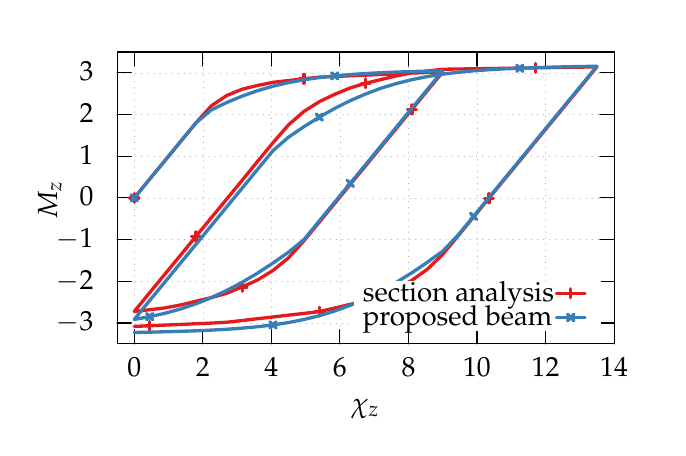
\begin{tikzpicture}[gnuplot]
%% generated with GNUPLOT 5.4p3 (Lua 5.4; terminal rev. Jun 2020, script rev. 115)
%% 07/15/2022 22:55:18
\path (0.000,0.000) rectangle (8.000,5.000);
\gpcolor{color=gp lt color axes}
\gpsetlinetype{gp lt axes}
\gpsetdashtype{gp dt axes}
\gpsetlinewidth{0.50}
\draw[gp path] (1.136,1.250)--(4.139,1.250);
\draw[gp path] (7.263,1.250)--(7.447,1.250);
\gpcolor{color=gp lt color border}
\gpsetlinetype{gp lt border}
\gpsetdashtype{gp dt solid}
\gpsetlinewidth{1.00}
\draw[gp path] (1.136,1.250)--(1.316,1.250);
\draw[gp path] (7.447,1.250)--(7.267,1.250);
\node[gp node right] at (0.952,1.250) {$-3$};
\gpcolor{color=gp lt color axes}
\gpsetlinetype{gp lt axes}
\gpsetdashtype{gp dt axes}
\gpsetlinewidth{0.50}
\draw[gp path] (1.136,1.779)--(4.139,1.779);
\draw[gp path] (7.263,1.779)--(7.447,1.779);
\gpcolor{color=gp lt color border}
\gpsetlinetype{gp lt border}
\gpsetdashtype{gp dt solid}
\gpsetlinewidth{1.00}
\draw[gp path] (1.136,1.779)--(1.316,1.779);
\draw[gp path] (7.447,1.779)--(7.267,1.779);
\node[gp node right] at (0.952,1.779) {$-2$};
\gpcolor{color=gp lt color axes}
\gpsetlinetype{gp lt axes}
\gpsetdashtype{gp dt axes}
\gpsetlinewidth{0.50}
\draw[gp path] (1.136,2.309)--(7.447,2.309);
\gpcolor{color=gp lt color border}
\gpsetlinetype{gp lt border}
\gpsetdashtype{gp dt solid}
\gpsetlinewidth{1.00}
\draw[gp path] (1.136,2.309)--(1.316,2.309);
\draw[gp path] (7.447,2.309)--(7.267,2.309);
\node[gp node right] at (0.952,2.309) {$-1$};
\gpcolor{color=gp lt color axes}
\gpsetlinetype{gp lt axes}
\gpsetdashtype{gp dt axes}
\gpsetlinewidth{0.50}
\draw[gp path] (1.136,2.838)--(7.447,2.838);
\gpcolor{color=gp lt color border}
\gpsetlinetype{gp lt border}
\gpsetdashtype{gp dt solid}
\gpsetlinewidth{1.00}
\draw[gp path] (1.136,2.838)--(1.316,2.838);
\draw[gp path] (7.447,2.838)--(7.267,2.838);
\node[gp node right] at (0.952,2.838) {$0$};
\gpcolor{color=gp lt color axes}
\gpsetlinetype{gp lt axes}
\gpsetdashtype{gp dt axes}
\gpsetlinewidth{0.50}
\draw[gp path] (1.136,3.367)--(7.447,3.367);
\gpcolor{color=gp lt color border}
\gpsetlinetype{gp lt border}
\gpsetdashtype{gp dt solid}
\gpsetlinewidth{1.00}
\draw[gp path] (1.136,3.367)--(1.316,3.367);
\draw[gp path] (7.447,3.367)--(7.267,3.367);
\node[gp node right] at (0.952,3.367) {$1$};
\gpcolor{color=gp lt color axes}
\gpsetlinetype{gp lt axes}
\gpsetdashtype{gp dt axes}
\gpsetlinewidth{0.50}
\draw[gp path] (1.136,3.897)--(7.447,3.897);
\gpcolor{color=gp lt color border}
\gpsetlinetype{gp lt border}
\gpsetdashtype{gp dt solid}
\gpsetlinewidth{1.00}
\draw[gp path] (1.136,3.897)--(1.316,3.897);
\draw[gp path] (7.447,3.897)--(7.267,3.897);
\node[gp node right] at (0.952,3.897) {$2$};
\gpcolor{color=gp lt color axes}
\gpsetlinetype{gp lt axes}
\gpsetdashtype{gp dt axes}
\gpsetlinewidth{0.50}
\draw[gp path] (1.136,4.426)--(7.447,4.426);
\gpcolor{color=gp lt color border}
\gpsetlinetype{gp lt border}
\gpsetdashtype{gp dt solid}
\gpsetlinewidth{1.00}
\draw[gp path] (1.136,4.426)--(1.316,4.426);
\draw[gp path] (7.447,4.426)--(7.267,4.426);
\node[gp node right] at (0.952,4.426) {$3$};
\gpcolor{color=gp lt color axes}
\gpsetlinetype{gp lt axes}
\gpsetdashtype{gp dt axes}
\gpsetlinewidth{0.50}
\draw[gp path] (1.354,0.985)--(1.354,4.691);
\gpcolor{color=gp lt color border}
\gpsetlinetype{gp lt border}
\gpsetdashtype{gp dt solid}
\gpsetlinewidth{1.00}
\draw[gp path] (1.354,0.985)--(1.354,1.165);
\draw[gp path] (1.354,4.691)--(1.354,4.511);
\node[gp node center] at (1.354,0.677) {$0$};
\gpcolor{color=gp lt color axes}
\gpsetlinetype{gp lt axes}
\gpsetdashtype{gp dt axes}
\gpsetlinewidth{0.50}
\draw[gp path] (2.224,0.985)--(2.224,4.691);
\gpcolor{color=gp lt color border}
\gpsetlinetype{gp lt border}
\gpsetdashtype{gp dt solid}
\gpsetlinewidth{1.00}
\draw[gp path] (2.224,0.985)--(2.224,1.165);
\draw[gp path] (2.224,4.691)--(2.224,4.511);
\node[gp node center] at (2.224,0.677) {$2$};
\gpcolor{color=gp lt color axes}
\gpsetlinetype{gp lt axes}
\gpsetdashtype{gp dt axes}
\gpsetlinewidth{0.50}
\draw[gp path] (3.095,0.985)--(3.095,4.691);
\gpcolor{color=gp lt color border}
\gpsetlinetype{gp lt border}
\gpsetdashtype{gp dt solid}
\gpsetlinewidth{1.00}
\draw[gp path] (3.095,0.985)--(3.095,1.165);
\draw[gp path] (3.095,4.691)--(3.095,4.511);
\node[gp node center] at (3.095,0.677) {$4$};
\gpcolor{color=gp lt color axes}
\gpsetlinetype{gp lt axes}
\gpsetdashtype{gp dt axes}
\gpsetlinewidth{0.50}
\draw[gp path] (3.965,0.985)--(3.965,4.691);
\gpcolor{color=gp lt color border}
\gpsetlinetype{gp lt border}
\gpsetdashtype{gp dt solid}
\gpsetlinewidth{1.00}
\draw[gp path] (3.965,0.985)--(3.965,1.165);
\draw[gp path] (3.965,4.691)--(3.965,4.511);
\node[gp node center] at (3.965,0.677) {$6$};
\gpcolor{color=gp lt color axes}
\gpsetlinetype{gp lt axes}
\gpsetdashtype{gp dt axes}
\gpsetlinewidth{0.50}
\draw[gp path] (4.836,0.985)--(4.836,1.165);
\draw[gp path] (4.836,1.781)--(4.836,4.691);
\gpcolor{color=gp lt color border}
\gpsetlinetype{gp lt border}
\gpsetdashtype{gp dt solid}
\gpsetlinewidth{1.00}
\draw[gp path] (4.836,0.985)--(4.836,1.165);
\draw[gp path] (4.836,4.691)--(4.836,4.511);
\node[gp node center] at (4.836,0.677) {$8$};
\gpcolor{color=gp lt color axes}
\gpsetlinetype{gp lt axes}
\gpsetdashtype{gp dt axes}
\gpsetlinewidth{0.50}
\draw[gp path] (5.706,0.985)--(5.706,1.165);
\draw[gp path] (5.706,1.781)--(5.706,4.691);
\gpcolor{color=gp lt color border}
\gpsetlinetype{gp lt border}
\gpsetdashtype{gp dt solid}
\gpsetlinewidth{1.00}
\draw[gp path] (5.706,0.985)--(5.706,1.165);
\draw[gp path] (5.706,4.691)--(5.706,4.511);
\node[gp node center] at (5.706,0.677) {$10$};
\gpcolor{color=gp lt color axes}
\gpsetlinetype{gp lt axes}
\gpsetdashtype{gp dt axes}
\gpsetlinewidth{0.50}
\draw[gp path] (6.577,0.985)--(6.577,1.165);
\draw[gp path] (6.577,1.781)--(6.577,4.691);
\gpcolor{color=gp lt color border}
\gpsetlinetype{gp lt border}
\gpsetdashtype{gp dt solid}
\gpsetlinewidth{1.00}
\draw[gp path] (6.577,0.985)--(6.577,1.165);
\draw[gp path] (6.577,4.691)--(6.577,4.511);
\node[gp node center] at (6.577,0.677) {$12$};
\gpcolor{color=gp lt color axes}
\gpsetlinetype{gp lt axes}
\gpsetdashtype{gp dt axes}
\gpsetlinewidth{0.50}
\draw[gp path] (7.447,0.985)--(7.447,4.691);
\gpcolor{color=gp lt color border}
\gpsetlinetype{gp lt border}
\gpsetdashtype{gp dt solid}
\gpsetlinewidth{1.00}
\draw[gp path] (7.447,0.985)--(7.447,1.165);
\draw[gp path] (7.447,4.691)--(7.447,4.511);
\node[gp node center] at (7.447,0.677) {$14$};
\draw[gp path] (1.136,4.691)--(1.136,0.985)--(7.447,0.985)--(7.447,4.691)--cycle;
\node[gp node center,rotate=-270] at (0.292,2.838) {$M_z$};
\node[gp node center] at (4.291,0.215) {$\chi_z$};
\gpcolor{rgb color={0.894,0.102,0.110}}
\gpsetlinewidth{3.00}
\draw[gp path] (1.354,2.838)--(1.549,3.076)--(1.745,3.314)--(1.941,3.553)--(2.137,3.791)%
  --(2.333,4.008)--(2.529,4.139)--(2.725,4.219)--(2.920,4.266)--(3.116,4.306)--(3.312,4.328)%
  --(3.508,4.351)--(3.704,4.372)--(3.900,4.380)--(4.096,4.389)--(4.292,4.397)--(4.487,4.406)%
  --(4.683,4.414)--(4.879,4.423)--(5.075,4.431)--(5.271,4.437)--(5.075,4.199)--(4.879,3.961)%
  --(4.683,3.722)--(4.487,3.484)--(4.292,3.246)--(4.096,3.008)--(3.900,2.769)--(3.704,2.531)%
  --(3.508,2.293)--(3.312,2.076)--(3.116,1.917)--(2.920,1.796)--(2.725,1.708)--(2.529,1.627)%
  --(2.333,1.572)--(2.137,1.525)--(1.941,1.478)--(1.745,1.441)--(1.549,1.418)--(1.354,1.396)%
  --(1.549,1.634)--(1.745,1.872)--(1.941,2.110)--(2.137,2.349)--(2.333,2.587)--(2.529,2.825)%
  --(2.725,3.063)--(2.920,3.302)--(3.116,3.540)--(3.312,3.765)--(3.508,3.936)--(3.704,4.060)%
  --(3.900,4.154)--(4.096,4.235)--(4.292,4.294)--(4.487,4.341)--(4.683,4.388)--(4.879,4.426)%
  --(5.075,4.449)--(5.271,4.472)--(5.467,4.475)--(5.663,4.478)--(5.858,4.481)--(6.054,4.484)%
  --(6.250,4.487)--(6.446,4.490)--(6.642,4.493)--(6.838,4.496)--(7.034,4.499)--(7.229,4.502)%
  --(7.034,4.263)--(6.838,4.025)--(6.642,3.787)--(6.446,3.549)--(6.250,3.310)--(6.054,3.072)%
  --(5.858,2.834)--(5.663,2.596)--(5.467,2.357)--(5.271,2.121)--(5.075,1.931)--(4.879,1.791)%
  --(4.683,1.683)--(4.487,1.602)--(4.292,1.533)--(4.096,1.486)--(3.900,1.439)--(3.704,1.394)%
  --(3.508,1.371)--(3.312,1.349)--(3.116,1.326)--(2.920,1.304)--(2.725,1.281)--(2.529,1.259)%
  --(2.333,1.248)--(2.137,1.240)--(1.941,1.231)--(1.745,1.223)--(1.549,1.214)--(1.354,1.206);
\gpsetpointsize{4.00}
\gp3point{gp mark 1}{}{(1.354,2.838)}
\gp3point{gp mark 1}{}{(3.508,4.351)}
\gp3point{gp mark 1}{}{(4.879,3.961)}
\gp3point{gp mark 1}{}{(2.725,1.708)}
\gp3point{gp mark 1}{}{(2.137,2.349)}
\gp3point{gp mark 1}{}{(4.292,4.294)}
\gp3point{gp mark 1}{}{(6.446,4.490)}
\gp3point{gp mark 1}{}{(5.858,2.834)}
\gp3point{gp mark 1}{}{(3.704,1.394)}
\gp3point{gp mark 1}{}{(1.549,1.214)}
\gpcolor{rgb color={0.216,0.494,0.722}}
\draw[gp path] (1.354,2.838)--(1.549,3.076)--(1.745,3.314)--(1.941,3.553)--(2.137,3.791)%
  --(2.333,3.956)--(2.529,4.050)--(2.725,4.131)--(2.920,4.200)--(3.116,4.257)--(3.312,4.302)%
  --(3.508,4.338)--(3.704,4.366)--(3.900,4.388)--(4.096,4.405)--(4.292,4.418)--(4.487,4.428)%
  --(4.683,4.436)--(4.879,4.443)--(5.075,4.448)--(5.271,4.452)--(5.075,4.214)--(4.879,3.976)%
  --(4.683,3.738)--(4.487,3.499)--(4.292,3.261)--(4.096,3.023)--(3.900,2.785)--(3.704,2.546)%
  --(3.508,2.308)--(3.312,2.148)--(3.116,2.011)--(2.920,1.883)--(2.725,1.767)--(2.529,1.663)%
  --(2.333,1.572)--(2.137,1.493)--(1.941,1.427)--(1.745,1.373)--(1.549,1.330)--(1.354,1.295)%
  --(1.549,1.534)--(1.745,1.772)--(1.941,2.010)--(2.137,2.248)--(2.333,2.487)--(2.529,2.725)%
  --(2.725,2.963)--(2.920,3.201)--(3.116,3.439)--(3.312,3.609)--(3.508,3.742)--(3.704,3.864)%
  --(3.900,3.975)--(4.096,4.073)--(4.292,4.158)--(4.487,4.231)--(4.683,4.291)--(4.879,4.340)%
  --(5.075,4.379)--(5.271,4.410)--(5.467,4.433)--(5.663,4.452)--(5.858,4.466)--(6.054,4.477)%
  --(6.250,4.485)--(6.446,4.492)--(6.642,4.498)--(6.838,4.503)--(7.034,4.507)--(7.229,4.510)%
  --(7.034,4.272)--(6.838,4.034)--(6.642,3.795)--(6.446,3.557)--(6.250,3.319)--(6.054,3.081)%
  --(5.858,2.842)--(5.663,2.604)--(5.467,2.366)--(5.271,2.161)--(5.075,2.020)--(4.879,1.887)%
  --(4.683,1.766)--(4.487,1.656)--(4.292,1.558)--(4.096,1.474)--(3.900,1.402)--(3.704,1.342)%
  --(3.508,1.294)--(3.312,1.255)--(3.116,1.225)--(2.920,1.202)--(2.725,1.184)--(2.529,1.170)%
  --(2.333,1.159)--(2.137,1.150)--(1.941,1.144)--(1.745,1.138)--(1.549,1.133)--(1.354,1.129);
\gp3point{gp mark 2}{}{(1.354,2.838)}
\gp3point{gp mark 2}{}{(3.900,4.388)}
\gp3point{gp mark 2}{}{(4.096,3.023)}
\gp3point{gp mark 2}{}{(1.549,1.330)}
\gp3point{gp mark 2}{}{(3.704,3.864)}
\gp3point{gp mark 2}{}{(6.250,4.485)}
\gp3point{gp mark 2}{}{(5.663,2.604)}
\gp3point{gp mark 2}{}{(3.116,1.225)}
\gpfill{color=gpbgfillcolor} (4.139,1.165)--(7.263,1.165)--(7.263,1.781)--(4.139,1.781)--cycle;
\gpcolor{color=gp lt color border}
\node[gp node left] at (4.139,1.627) {section analysis};
\gpcolor{rgb color={0.894,0.102,0.110}}
\draw[gp path] (6.715,1.627)--(7.079,1.627);
\gp3point{gp mark 1}{}{(6.897,1.627)}
\gpcolor{color=gp lt color border}
\node[gp node left] at (4.139,1.319) {proposed beam};
\gpcolor{rgb color={0.216,0.494,0.722}}
\draw[gp path] (6.715,1.319)--(7.079,1.319);
\gp3point{gp mark 2}{}{(6.897,1.319)}
\gpcolor{color=gp lt color border}
\gpsetlinewidth{1.00}
\draw[gp path] (1.136,4.691)--(1.136,0.985)--(7.447,0.985)--(7.447,4.691)--cycle;
%% coordinates of the plot area
\gpdefrectangularnode{gp plot 1}{\pgfpoint{1.136cm}{0.985cm}}{\pgfpoint{7.447cm}{4.691cm}}
\end{tikzpicture}
%% gnuplot variables

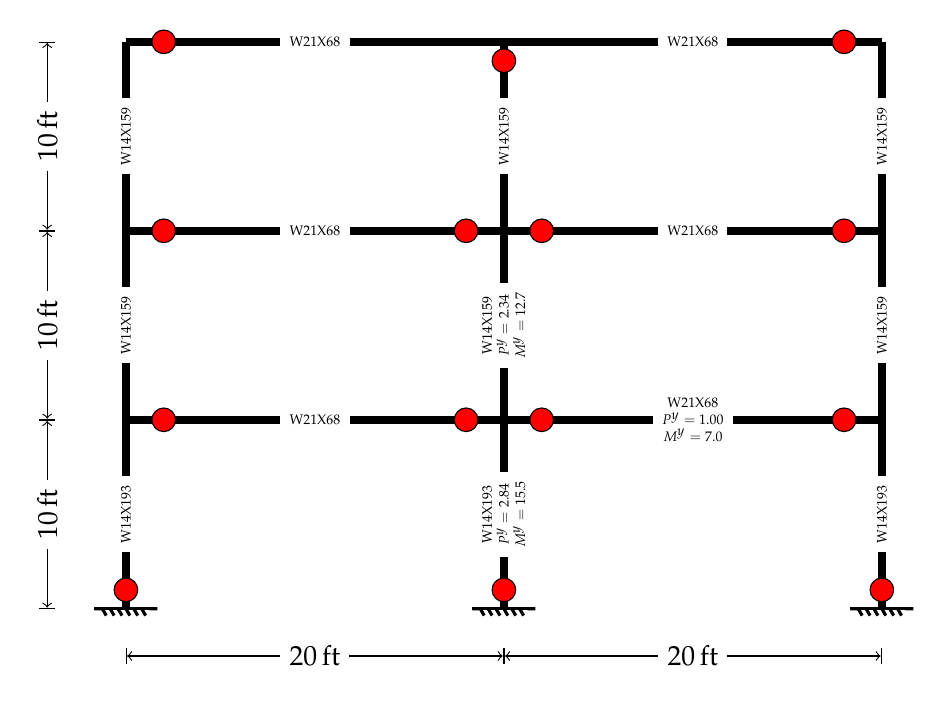
\begin{tikzpicture}[scale=2]
\coordinate(N1)at(0.0,0.0);
\coordinate(N2)at(0.0,1.2);
\coordinate(N3)at(0.0,2.4);
\coordinate(N4)at(0.0,3.6);
\coordinate(N5)at(2.4,0.0);
\coordinate(N6)at(2.4,1.2);
\coordinate(N7)at(2.4,2.4);
\coordinate(N8)at(2.4,3.6);
\coordinate(N9)at(4.8,0.0);
\coordinate(N10)at(4.8,1.2);
\coordinate(N11)at(4.8,2.4);
\coordinate(N12)at(4.8,3.6);
\draw[line width=1mm](N2)--(N6)node[midway,fill=white,font=\tiny]{W21X68};
\draw[line width=1mm](N6)--(N10)node[midway,fill=white,font=\tiny,align=center]{W21X68\\$P^y=1.00$\\$M^y=7.0$};
\draw[line width=1mm](N3)--(N7)node[midway,fill=white,font=\tiny]{W21X68};
\draw[line width=1mm](N7)--(N11)node[midway,fill=white,font=\tiny]{W21X68};
\draw[line width=1mm](N4)--(N8)node[midway,fill=white,font=\tiny]{W21X68};
\draw[line width=1mm](N8)--(N12)node[midway,fill=white,font=\tiny]{W21X68};
\draw[line width=1mm](N1)--(N2)node[midway,fill=white,font=\tiny,rotate=90]{W14X193};
\draw[line width=1mm](N5)--(N6)node[midway,fill=white,font=\tiny,rotate=90,align=center]{W14X193\\$P^y=2.84$\\$M^y=15.5$};
\draw[line width=1mm](N9)--(N10)node[midway,fill=white,font=\tiny,rotate=90]{W14X193};
\draw[line width=1mm](N2)--(N3)node[midway,fill=white,font=\tiny,rotate=90]{W14X159};
\draw[line width=1mm](N6)--(N7)node[midway,fill=white,font=\tiny,rotate=90,align=center]{W14X159\\$P^y=2.34$\\$M^y=12.7$};
\draw[line width=1mm](N10)--(N11)node[midway,fill=white,font=\tiny,rotate=90]{W14X159};
\draw[line width=1mm](N3)--(N4)node[midway,fill=white,font=\tiny,rotate=90]{W14X159};
\draw[line width=1mm](N7)--(N8)node[midway,fill=white,font=\tiny,rotate=90]{W14X159};
\draw[line width=1mm](N11)--(N12)node[midway,fill=white,font=\tiny,rotate=90]{W14X159};
\node[fill=red,circle,draw,inner sep=0,minimum size=3mm]at($(N2)!.1!(N6)$){};
\node[fill=red,circle,draw,inner sep=0,minimum size=3mm]at($(N2)!.9!(N6)$){};
\node[fill=red,circle,draw,inner sep=0,minimum size=3mm]at($(N7)!.9!(N8)$){};
\node[fill=red,circle,draw,inner sep=0,minimum size=3mm]at($(N6)!.1!(N10)$){};
\node[fill=red,circle,draw,inner sep=0,minimum size=3mm]at($(N6)!.9!(N10)$){};
\node[fill=red,circle,draw,inner sep=0,minimum size=3mm]at($(N3)!.1!(N7)$){};
\node[fill=red,circle,draw,inner sep=0,minimum size=3mm]at($(N3)!.9!(N7)$){};
\node[fill=red,circle,draw,inner sep=0,minimum size=3mm]at($(N7)!.1!(N11)$){};
\node[fill=red,circle,draw,inner sep=0,minimum size=3mm]at($(N7)!.9!(N11)$){};
\node[fill=red,circle,draw,inner sep=0,minimum size=3mm]at($(N4)!.1!(N8)$){};
\node[fill=red,circle,draw,inner sep=0,minimum size=3mm]at($(N8)!.9!(N12)$){};
\node[fill=red,circle,draw,inner sep=0,minimum size=3mm]at($(N1)!.1!(N2)$){};
\node[fill=red,circle,draw,inner sep=0,minimum size=3mm]at($(N5)!.1!(N6)$){};
\node[fill=red,circle,draw,inner sep=0,minimum size=3mm]at($(N9)!.1!(N10)$){};
\FixedSupport{N1}{.5}
\FixedSupport{N5}{.5}
\FixedSupport{N9}{.5}
\draw[|<->|]($(N1)-(0,.3)$)--($(N5)-(0,.3)$)node[midway,fill=white]{\SI{20}{ft}};
\draw[|<->|]($(N5)-(0,.3)$)--($(N9)-(0,.3)$)node[midway,fill=white]{\SI{20}{ft}};
\draw[|<->|]($(N1)-(.5,0)$)--($(N2)-(.5,0)$)node[midway,fill=white,rotate=90]{\SI{10}{ft}};
\draw[|<->|]($(N2)-(.5,0)$)--($(N3)-(.5,0)$)node[midway,fill=white,rotate=90]{\SI{10}{ft}};
\draw[|<->|]($(N3)-(.5,0)$)--($(N4)-(.5,0)$)node[midway,fill=white,rotate=90]{\SI{10}{ft}};
\end{tikzpicture}

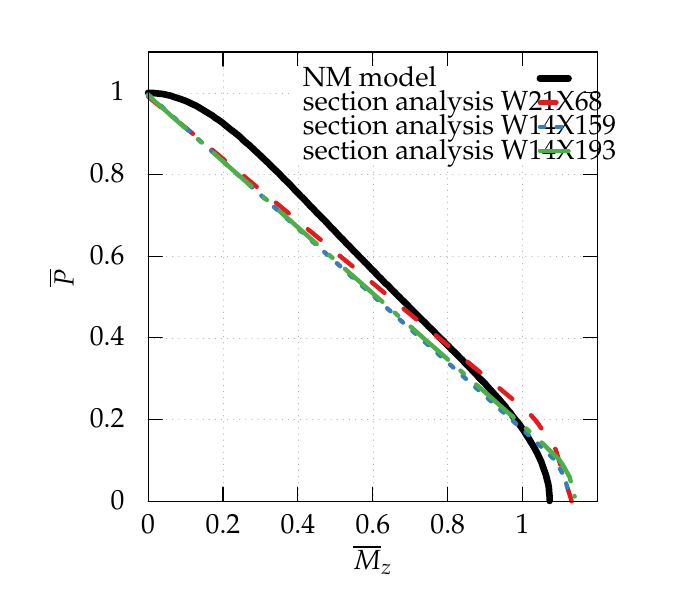
\begin{tikzpicture}[gnuplot]
%% generated with GNUPLOT 5.4p5 (Lua 5.4; terminal rev. Jun 2020, script rev. 115)
%% 05/22/23 00:52:11
\path (0.000,0.000) rectangle (8.000,7.000);
\gpcolor{color=gp lt color axes}
\gpsetlinetype{gp lt axes}
\gpsetdashtype{gp dt axes}
\gpsetlinewidth{0.50}
\draw[gp path] (1.530,0.985)--(7.237,0.985);
\gpcolor{color=gp lt color border}
\gpsetlinetype{gp lt border}
\gpsetdashtype{gp dt solid}
\gpsetlinewidth{1.00}
\draw[gp path] (1.530,0.985)--(1.710,0.985);
\draw[gp path] (7.237,0.985)--(7.057,0.985);
\node[gp node right] at (1.346,0.985) {$0$};
\gpcolor{color=gp lt color axes}
\gpsetlinetype{gp lt axes}
\gpsetdashtype{gp dt axes}
\gpsetlinewidth{0.50}
\draw[gp path] (1.530,2.022)--(7.237,2.022);
\gpcolor{color=gp lt color border}
\gpsetlinetype{gp lt border}
\gpsetdashtype{gp dt solid}
\gpsetlinewidth{1.00}
\draw[gp path] (1.530,2.022)--(1.710,2.022);
\draw[gp path] (7.237,2.022)--(7.057,2.022);
\node[gp node right] at (1.346,2.022) {$0.2$};
\gpcolor{color=gp lt color axes}
\gpsetlinetype{gp lt axes}
\gpsetdashtype{gp dt axes}
\gpsetlinewidth{0.50}
\draw[gp path] (1.530,3.060)--(7.237,3.060);
\gpcolor{color=gp lt color border}
\gpsetlinetype{gp lt border}
\gpsetdashtype{gp dt solid}
\gpsetlinewidth{1.00}
\draw[gp path] (1.530,3.060)--(1.710,3.060);
\draw[gp path] (7.237,3.060)--(7.057,3.060);
\node[gp node right] at (1.346,3.060) {$0.4$};
\gpcolor{color=gp lt color axes}
\gpsetlinetype{gp lt axes}
\gpsetdashtype{gp dt axes}
\gpsetlinewidth{0.50}
\draw[gp path] (1.530,4.097)--(7.237,4.097);
\gpcolor{color=gp lt color border}
\gpsetlinetype{gp lt border}
\gpsetdashtype{gp dt solid}
\gpsetlinewidth{1.00}
\draw[gp path] (1.530,4.097)--(1.710,4.097);
\draw[gp path] (7.237,4.097)--(7.057,4.097);
\node[gp node right] at (1.346,4.097) {$0.6$};
\gpcolor{color=gp lt color axes}
\gpsetlinetype{gp lt axes}
\gpsetdashtype{gp dt axes}
\gpsetlinewidth{0.50}
\draw[gp path] (1.530,5.135)--(7.237,5.135);
\gpcolor{color=gp lt color border}
\gpsetlinetype{gp lt border}
\gpsetdashtype{gp dt solid}
\gpsetlinewidth{1.00}
\draw[gp path] (1.530,5.135)--(1.710,5.135);
\draw[gp path] (7.237,5.135)--(7.057,5.135);
\node[gp node right] at (1.346,5.135) {$0.8$};
\gpcolor{color=gp lt color axes}
\gpsetlinetype{gp lt axes}
\gpsetdashtype{gp dt axes}
\gpsetlinewidth{0.50}
\draw[gp path] (1.530,6.172)--(3.377,6.172);
\draw[gp path] (7.053,6.172)--(7.237,6.172);
\gpcolor{color=gp lt color border}
\gpsetlinetype{gp lt border}
\gpsetdashtype{gp dt solid}
\gpsetlinewidth{1.00}
\draw[gp path] (1.530,6.172)--(1.710,6.172);
\draw[gp path] (7.237,6.172)--(7.057,6.172);
\node[gp node right] at (1.346,6.172) {$1$};
\gpcolor{color=gp lt color axes}
\gpsetlinetype{gp lt axes}
\gpsetdashtype{gp dt axes}
\gpsetlinewidth{0.50}
\draw[gp path] (1.530,0.985)--(1.530,6.691);
\gpcolor{color=gp lt color border}
\gpsetlinetype{gp lt border}
\gpsetdashtype{gp dt solid}
\gpsetlinewidth{1.00}
\draw[gp path] (1.530,0.985)--(1.530,1.165);
\draw[gp path] (1.530,6.691)--(1.530,6.511);
\node[gp node center] at (1.530,0.677) {$0$};
\gpcolor{color=gp lt color axes}
\gpsetlinetype{gp lt axes}
\gpsetdashtype{gp dt axes}
\gpsetlinewidth{0.50}
\draw[gp path] (2.481,0.985)--(2.481,6.691);
\gpcolor{color=gp lt color border}
\gpsetlinetype{gp lt border}
\gpsetdashtype{gp dt solid}
\gpsetlinewidth{1.00}
\draw[gp path] (2.481,0.985)--(2.481,1.165);
\draw[gp path] (2.481,6.691)--(2.481,6.511);
\node[gp node center] at (2.481,0.677) {$0.2$};
\gpcolor{color=gp lt color axes}
\gpsetlinetype{gp lt axes}
\gpsetdashtype{gp dt axes}
\gpsetlinewidth{0.50}
\draw[gp path] (3.432,0.985)--(3.432,5.279);
\draw[gp path] (3.432,6.511)--(3.432,6.691);
\gpcolor{color=gp lt color border}
\gpsetlinetype{gp lt border}
\gpsetdashtype{gp dt solid}
\gpsetlinewidth{1.00}
\draw[gp path] (3.432,0.985)--(3.432,1.165);
\draw[gp path] (3.432,6.691)--(3.432,6.511);
\node[gp node center] at (3.432,0.677) {$0.4$};
\gpcolor{color=gp lt color axes}
\gpsetlinetype{gp lt axes}
\gpsetdashtype{gp dt axes}
\gpsetlinewidth{0.50}
\draw[gp path] (4.384,0.985)--(4.384,5.279);
\draw[gp path] (4.384,6.511)--(4.384,6.691);
\gpcolor{color=gp lt color border}
\gpsetlinetype{gp lt border}
\gpsetdashtype{gp dt solid}
\gpsetlinewidth{1.00}
\draw[gp path] (4.384,0.985)--(4.384,1.165);
\draw[gp path] (4.384,6.691)--(4.384,6.511);
\node[gp node center] at (4.384,0.677) {$0.6$};
\gpcolor{color=gp lt color axes}
\gpsetlinetype{gp lt axes}
\gpsetdashtype{gp dt axes}
\gpsetlinewidth{0.50}
\draw[gp path] (5.335,0.985)--(5.335,5.279);
\draw[gp path] (5.335,6.511)--(5.335,6.691);
\gpcolor{color=gp lt color border}
\gpsetlinetype{gp lt border}
\gpsetdashtype{gp dt solid}
\gpsetlinewidth{1.00}
\draw[gp path] (5.335,0.985)--(5.335,1.165);
\draw[gp path] (5.335,6.691)--(5.335,6.511);
\node[gp node center] at (5.335,0.677) {$0.8$};
\gpcolor{color=gp lt color axes}
\gpsetlinetype{gp lt axes}
\gpsetdashtype{gp dt axes}
\gpsetlinewidth{0.50}
\draw[gp path] (6.286,0.985)--(6.286,5.279);
\draw[gp path] (6.286,6.511)--(6.286,6.691);
\gpcolor{color=gp lt color border}
\gpsetlinetype{gp lt border}
\gpsetdashtype{gp dt solid}
\gpsetlinewidth{1.00}
\draw[gp path] (6.286,0.985)--(6.286,1.165);
\draw[gp path] (6.286,6.691)--(6.286,6.511);
\node[gp node center] at (6.286,0.677) {$1$};
\draw[gp path] (1.530,6.691)--(1.530,0.985)--(7.237,0.985)--(7.237,6.691)--cycle;
\node[gp node center,rotate=-270] at (0.502,3.838) {$\overline{P}$};
\node[gp node center] at (4.383,0.215) {$\overline{M}_z$};
\gpcolor{rgb color={0.000,0.000,0.000}}
\gpsetlinewidth{6.00}
\draw[gp path] (1.530,6.172)--(1.578,6.172)--(1.625,6.167)--(1.673,6.162)--(1.720,6.157)%
  --(1.768,6.146)--(1.815,6.136)--(1.858,6.120)--(1.906,6.105)--(1.953,6.089)--(1.996,6.074)%
  --(2.044,6.053)--(2.086,6.032)--(2.134,6.011)--(2.177,5.986)--(2.220,5.960)--(2.262,5.934)%
  --(2.305,5.908)--(2.348,5.882)--(2.386,5.851)--(2.429,5.825)--(2.472,5.794)--(2.510,5.762)%
  --(2.548,5.731)--(2.586,5.700)--(2.629,5.669)--(2.667,5.638)--(2.705,5.607)--(2.738,5.571)%
  --(2.776,5.539)--(2.814,5.508)--(2.847,5.477)--(2.885,5.441)--(2.919,5.410)--(2.952,5.379)%
  --(2.990,5.342)--(3.023,5.311)--(3.057,5.280)--(3.090,5.244)--(3.123,5.213)--(3.156,5.182)%
  --(3.190,5.150)--(3.223,5.114)--(3.252,5.083)--(3.285,5.052)--(3.318,5.021)--(3.347,4.990)%
  --(3.380,4.953)--(3.409,4.922)--(3.442,4.891)--(3.470,4.860)--(3.504,4.829)--(3.532,4.798)%
  --(3.561,4.767)--(3.589,4.735)--(3.623,4.704)--(3.651,4.673)--(3.680,4.642)--(3.708,4.616)%
  --(3.737,4.585)--(3.770,4.554)--(3.799,4.523)--(3.827,4.492)--(3.856,4.460)--(3.884,4.435)%
  --(3.913,4.403)--(3.941,4.372)--(3.970,4.341)--(3.998,4.315)--(4.027,4.284)--(4.055,4.253)%
  --(4.084,4.227)--(4.112,4.196)--(4.141,4.165)--(4.169,4.139)--(4.198,4.108)--(4.227,4.077)%
  --(4.255,4.051)--(4.284,4.020)--(4.312,3.994)--(4.341,3.962)--(4.369,3.931)--(4.398,3.905)%
  --(4.426,3.874)--(4.455,3.843)--(4.483,3.817)--(4.512,3.786)--(4.540,3.755)--(4.574,3.729)%
  --(4.602,3.698)--(4.631,3.667)--(4.659,3.641)--(4.688,3.610)--(4.721,3.579)--(4.750,3.548)%
  --(4.778,3.522)--(4.812,3.490)--(4.840,3.459)--(4.869,3.428)--(4.902,3.397)--(4.930,3.366)%
  --(4.964,3.335)--(4.992,3.304)--(5.026,3.273)--(5.059,3.241)--(5.087,3.210)--(5.121,3.179)%
  --(5.154,3.148)--(5.182,3.117)--(5.216,3.081)--(5.249,3.050)--(5.282,3.018)--(5.316,2.982)%
  --(5.349,2.951)--(5.382,2.915)--(5.416,2.884)--(5.454,2.847)--(5.487,2.811)--(5.520,2.780)%
  --(5.553,2.743)--(5.591,2.707)--(5.625,2.671)--(5.658,2.635)--(5.696,2.598)--(5.729,2.557)%
  --(5.767,2.520)--(5.805,2.484)--(5.839,2.443)--(5.877,2.401)--(5.910,2.365)--(5.948,2.323)%
  --(5.986,2.282)--(6.020,2.240)--(6.058,2.199)--(6.091,2.152)--(6.129,2.111)--(6.162,2.064)%
  --(6.195,2.022)--(6.234,1.976)--(6.267,1.929)--(6.300,1.882)--(6.329,1.836)--(6.362,1.784)%
  --(6.390,1.737)--(6.424,1.685)--(6.448,1.639)--(6.476,1.587)--(6.500,1.535)--(6.524,1.483)%
  --(6.543,1.426)--(6.562,1.374)--(6.581,1.322)--(6.595,1.265)--(6.609,1.213)--(6.619,1.156)%
  --(6.623,1.099)--(6.628,1.047)--(6.628,0.990);
\gpcolor{rgb color={0.894,0.102,0.110}}
\gpsetdashtype{gp dt 3}
\gpsetlinewidth{4.00}
\draw[gp path] (1.530,6.124)--(1.544,6.112)--(1.559,6.100)--(1.573,6.088)--(1.587,6.076)%
  --(1.602,6.064)--(1.616,6.052)--(1.630,6.041)--(1.645,6.029)--(1.659,6.017)--(1.673,6.005)%
  --(1.817,5.886)--(1.960,5.767)--(2.104,5.648)--(2.247,5.529)--(2.391,5.409)--(2.534,5.290)%
  --(2.678,5.171)--(2.821,5.052)--(2.964,4.933)--(3.108,4.814)--(3.252,4.695)--(3.395,4.576)%
  --(3.538,4.457)--(3.682,4.338)--(3.825,4.219)--(3.968,4.099)--(4.112,3.981)--(4.256,3.861)%
  --(4.399,3.742)--(4.542,3.623)--(4.686,3.504)--(4.829,3.385)--(4.973,3.266)--(5.117,3.147)%
  --(5.260,3.028)--(5.403,2.908)--(5.547,2.790)--(5.690,2.670)--(5.833,2.552)--(5.977,2.432)%
  --(6.121,2.313)--(6.264,2.194)--(6.355,2.113)--(6.407,2.062)--(6.435,2.030)--(6.462,1.998)%
  --(6.483,1.971)--(6.498,1.949)--(6.513,1.926)--(6.528,1.905)--(6.543,1.882)--(6.558,1.861)%
  --(6.573,1.838)--(6.587,1.817)--(6.602,1.794)--(6.617,1.772)--(6.632,1.750)--(6.648,1.728)%
  --(6.663,1.706)--(6.678,1.684)--(6.693,1.662)--(6.706,1.642)--(6.708,1.635)--(6.710,1.628)%
  --(6.712,1.621)--(6.715,1.614)--(6.717,1.607)--(6.719,1.600)--(6.721,1.593)--(6.723,1.586)%
  --(6.725,1.579)--(6.727,1.572)--(6.729,1.565)--(6.732,1.558)--(6.734,1.551)--(6.736,1.544)%
  --(6.738,1.536)--(6.740,1.530)--(6.743,1.522)--(6.745,1.516)--(6.747,1.508)--(6.749,1.501)%
  --(6.751,1.494)--(6.753,1.487)--(6.756,1.480)--(6.758,1.473)--(6.760,1.466)--(6.762,1.459)%
  --(6.764,1.452)--(6.767,1.445)--(6.769,1.438)--(6.771,1.431)--(6.773,1.424)--(6.775,1.417)%
  --(6.778,1.410)--(6.780,1.403)--(6.782,1.396)--(6.784,1.389)--(6.786,1.382)--(6.788,1.375)%
  --(6.791,1.368)--(6.793,1.361)--(6.795,1.354)--(6.797,1.347)--(6.799,1.340)--(6.802,1.333)%
  --(6.804,1.326)--(6.806,1.319)--(6.808,1.312)--(6.810,1.305)--(6.812,1.298)--(6.814,1.291)%
  --(6.816,1.284)--(6.818,1.277)--(6.821,1.270)--(6.823,1.263)--(6.825,1.256)--(6.827,1.248)%
  --(6.829,1.241)--(6.831,1.234)--(6.833,1.227)--(6.836,1.220)--(6.838,1.213)--(6.840,1.206)%
  --(6.842,1.199)--(6.844,1.192)--(6.847,1.185)--(6.849,1.178)--(6.851,1.171)--(6.853,1.164)%
  --(6.855,1.157)--(6.858,1.150)--(6.860,1.143)--(6.862,1.136)--(6.864,1.129)--(6.866,1.122)%
  --(6.868,1.115)--(6.871,1.108)--(6.873,1.101)--(6.875,1.094)--(6.877,1.087)--(6.879,1.080)%
  --(6.882,1.073)--(6.884,1.066)--(6.886,1.059)--(6.888,1.052)--(6.890,1.045)--(6.893,1.038)%
  --(6.895,1.031)--(6.897,1.024)--(6.899,1.017)--(6.901,1.010)--(6.903,1.002)--(6.905,0.995)%
  --(6.907,0.988)--(6.908,0.985);
\gpcolor{rgb color={0.216,0.494,0.722}}
\gpsetdashtype{gp dt 4}
\draw[gp path] (1.530,6.152)--(1.540,6.143)--(1.551,6.135)--(1.561,6.126)--(1.571,6.117)%
  --(1.582,6.108)--(1.592,6.099)--(1.602,6.088)--(1.612,6.079)--(1.623,6.070)--(1.633,6.061)%
  --(1.736,5.968)--(1.839,5.877)--(1.943,5.784)--(2.046,5.692)--(2.149,5.599)--(2.252,5.508)%
  --(2.355,5.415)--(2.458,5.321)--(2.561,5.230)--(2.665,5.137)--(2.768,5.046)--(2.871,4.953)%
  --(2.974,4.862)--(3.077,4.768)--(3.180,4.677)--(3.283,4.584)--(3.386,4.491)--(3.490,4.399)%
  --(3.593,4.306)--(3.696,4.215)--(3.799,4.122)--(3.902,4.031)--(4.005,3.937)--(4.108,3.844)%
  --(4.212,3.753)--(4.315,3.660)--(4.418,3.569)--(4.521,3.475)--(4.624,3.384)--(4.727,3.291)%
  --(4.830,3.199)--(4.934,3.107)--(5.037,3.014)--(5.140,2.922)--(5.243,2.830)--(5.346,2.737)%
  --(5.451,2.645)--(5.552,2.553)--(5.657,2.460)--(5.758,2.368)--(5.863,2.276)--(5.964,2.183)%
  --(6.069,2.091)--(6.170,1.999)--(6.275,1.906)--(6.376,1.814)--(6.458,1.740)--(6.507,1.691)%
  --(6.559,1.642)--(6.608,1.593)--(6.660,1.544)--(6.690,1.513)--(6.698,1.503)--(6.702,1.493)%
  --(6.709,1.484)--(6.716,1.474)--(6.724,1.464)--(6.728,1.456)--(6.731,1.449)--(6.735,1.442)%
  --(6.739,1.436)--(6.743,1.429)--(6.746,1.422)--(6.750,1.415)--(6.754,1.409)--(6.758,1.402)%
  --(6.761,1.395)--(6.765,1.389)--(6.769,1.382)--(6.773,1.375)--(6.776,1.369)--(6.780,1.362)%
  --(6.784,1.355)--(6.788,1.348)--(6.791,1.342)--(6.795,1.335)--(6.799,1.328)--(6.803,1.322)%
  --(6.806,1.315)--(6.810,1.308)--(6.814,1.302)--(6.818,1.296)--(6.818,1.294)--(6.818,1.292)%
  --(6.818,1.290)--(6.821,1.288)--(6.821,1.286)--(6.821,1.284)--(6.821,1.282)--(6.821,1.280)%
  --(6.821,1.277)--(6.821,1.275)--(6.825,1.273)--(6.825,1.271)--(6.825,1.269)--(6.825,1.267)%
  --(6.825,1.264)--(6.825,1.262)--(6.825,1.260)--(6.829,1.258)--(6.829,1.256)--(6.829,1.254)%
  --(6.829,1.252)--(6.829,1.250)--(6.829,1.248)--(6.829,1.245)--(6.833,1.243)--(6.833,1.241)%
  --(6.833,1.239)--(6.833,1.237)--(6.833,1.235)--(6.833,1.232)--(6.833,1.230)--(6.836,1.228)%
  --(6.836,1.226)--(6.836,1.224)--(6.836,1.222)--(6.836,1.220)--(6.836,1.218)--(6.836,1.215)%
  --(6.840,1.213)--(6.840,1.211)--(6.840,1.209)--(6.840,1.207)--(6.840,1.205)--(6.840,1.203)%
  --(6.844,1.201)--(6.844,1.198)--(6.844,1.196)--(6.844,1.194)--(6.844,1.192)--(6.844,1.190)%
  --(6.844,1.188)--(6.848,1.186)--(6.848,1.183)--(6.848,1.181)--(6.848,1.179)--(6.848,1.177)%
  --(6.848,1.175)--(6.848,1.173)--(6.851,1.171)--(6.851,1.169)--(6.851,1.166)--(6.851,1.164)%
  --(6.851,1.162)--(6.851,1.160)--(6.851,1.158)--(6.855,1.156)--(6.855,1.154)--(6.855,1.151)%
  --(6.855,1.149)--(6.855,1.147)--(6.855,1.145)--(6.855,1.143)--(6.859,1.141)--(6.859,1.139)%
  --(6.859,1.137)--(6.859,1.134)--(6.859,1.132)--(6.859,1.130)--(6.859,1.128)--(6.863,1.126)%
  --(6.863,1.124)--(6.863,1.122)--(6.863,1.119)--(6.863,1.117)--(6.863,1.115)--(6.863,1.113)%
  --(6.866,1.111)--(6.866,1.109)--(6.866,1.107)--(6.866,1.105)--(6.866,1.102)--(6.866,1.100)%
  --(6.866,1.098)--(6.870,1.096)--(6.870,1.094)--(6.870,1.092)--(6.870,1.090)--(6.870,1.087)%
  --(6.870,1.085)--(6.870,1.083)--(6.874,1.081)--(6.874,1.079)--(6.874,1.077)--(6.874,1.075)%
  --(6.874,1.073)--(6.874,1.070)--(6.874,1.068)--(6.878,1.066)--(6.878,1.064)--(6.878,1.062)%
  --(6.878,1.060)--(6.878,1.058)--(6.878,1.055)--(6.878,1.053)--(6.881,1.051)--(6.881,1.049)%
  --(6.881,1.047);
\gpcolor{rgb color={0.302,0.686,0.290}}
\gpsetdashtype{gp dt 5}
\draw[gp path] (1.530,6.139)--(1.541,6.130)--(1.551,6.121)--(1.562,6.112)--(1.573,6.103)%
  --(1.583,6.094)--(1.594,6.085)--(1.604,6.074)--(1.615,6.065)--(1.626,6.055)--(1.636,6.046)%
  --(1.743,5.953)--(1.849,5.858)--(1.956,5.765)--(2.062,5.672)--(2.169,5.577)--(2.275,5.484)%
  --(2.381,5.391)--(2.488,5.296)--(2.594,5.202)--(2.700,5.109)--(2.807,5.014)--(2.913,4.921)%
  --(3.020,4.828)--(3.126,4.733)--(3.232,4.640)--(3.339,4.547)--(3.445,4.452)--(3.552,4.359)%
  --(3.658,4.265)--(3.764,4.170)--(3.871,4.077)--(3.977,3.984)--(4.083,3.889)--(4.190,3.796)%
  --(4.296,3.703)--(4.403,3.608)--(4.509,3.515)--(4.617,3.422)--(4.721,3.327)--(4.828,3.233)%
  --(4.936,3.140)--(5.040,3.045)--(5.148,2.952)--(5.255,2.859)--(5.359,2.765)--(5.467,2.671)%
  --(5.574,2.577)--(5.678,2.484)--(5.786,2.390)--(5.893,2.296)--(5.997,2.202)--(6.105,2.108)%
  --(6.212,2.015)--(6.317,1.921)--(6.424,1.827)--(6.491,1.764)--(6.544,1.715)--(6.593,1.666)%
  --(6.645,1.617)--(6.694,1.567)--(6.746,1.518)--(6.758,1.503)--(6.764,1.494)--(6.771,1.484)%
  --(6.777,1.475)--(6.786,1.465)--(6.792,1.456)--(6.795,1.447)--(6.801,1.441)--(6.804,1.434)%
  --(6.807,1.428)--(6.811,1.421)--(6.814,1.414)--(6.820,1.408)--(6.823,1.401)--(6.826,1.395)%
  --(6.829,1.388)--(6.832,1.382)--(6.838,1.375)--(6.841,1.368)--(6.844,1.362)--(6.847,1.355)%
  --(6.850,1.349)--(6.857,1.342)--(6.860,1.336)--(6.863,1.329)--(6.866,1.322)--(6.869,1.316)%
  --(6.875,1.309)--(6.878,1.303)--(6.881,1.296)--(6.884,1.291)--(6.884,1.289)--(6.884,1.287)%
  --(6.884,1.285)--(6.887,1.283)--(6.887,1.281)--(6.887,1.279)--(6.887,1.276)--(6.887,1.274)%
  --(6.887,1.272)--(6.890,1.270)--(6.890,1.268)--(6.890,1.266)--(6.890,1.264)--(6.890,1.262)%
  --(6.890,1.260)--(6.893,1.258)--(6.893,1.255)--(6.893,1.253)--(6.893,1.251)--(6.893,1.249)%
  --(6.893,1.247)--(6.896,1.245)--(6.896,1.243)--(6.896,1.241)--(6.896,1.239)--(6.896,1.237)%
  --(6.896,1.235)--(6.899,1.232)--(6.899,1.230)--(6.899,1.228)--(6.899,1.226)--(6.899,1.224)%
  --(6.903,1.222)--(6.903,1.220)--(6.903,1.218)--(6.903,1.216)--(6.903,1.213)--(6.903,1.211)%
  --(6.906,1.209)--(6.906,1.207)--(6.906,1.205)--(6.906,1.203)--(6.906,1.201)--(6.906,1.199)%
  --(6.909,1.197)--(6.909,1.195)--(6.909,1.192)--(6.909,1.190)--(6.909,1.188)--(6.909,1.186)%
  --(6.912,1.184)--(6.912,1.182)--(6.912,1.180)--(6.912,1.178)--(6.912,1.176)--(6.912,1.174)%
  --(6.915,1.171)--(6.915,1.169)--(6.915,1.167)--(6.915,1.165)--(6.915,1.163)--(6.918,1.161)%
  --(6.918,1.159)--(6.918,1.157)--(6.918,1.155)--(6.918,1.153)--(6.918,1.151)--(6.921,1.149)%
  --(6.921,1.146)--(6.921,1.144)--(6.921,1.142)--(6.921,1.140)--(6.921,1.138)--(6.924,1.136)%
  --(6.924,1.134)--(6.924,1.132)--(6.924,1.130)--(6.924,1.128)--(6.924,1.125)--(6.927,1.123)%
  --(6.927,1.121)--(6.927,1.119)--(6.927,1.117)--(6.927,1.115)--(6.930,1.113)--(6.930,1.111)%
  --(6.930,1.109)--(6.930,1.107)--(6.930,1.104)--(6.930,1.102)--(6.933,1.100)--(6.933,1.098)%
  --(6.933,1.096)--(6.933,1.094)--(6.933,1.092)--(6.933,1.090)--(6.936,1.088)--(6.936,1.086)%
  --(6.936,1.084)--(6.936,1.081)--(6.936,1.079)--(6.936,1.077)--(6.939,1.075)--(6.939,1.073)%
  --(6.939,1.071)--(6.939,1.069)--(6.939,1.067)--(6.939,1.065)--(6.942,1.063)--(6.942,1.060)%
  --(6.942,1.058)--(6.942,1.056)--(6.942,1.054)--(6.946,1.052)--(6.946,1.050)--(6.946,1.048)%
  --(6.946,1.046);
\gpfill{color=gpbgfillcolor} (3.377,5.279)--(7.053,5.279)--(7.053,6.511)--(3.377,6.511)--cycle;
\gpcolor{color=gp lt color border}
\node[gp node left] at (3.377,6.357) {NM model};
\gpcolor{rgb color={0.000,0.000,0.000}}
\gpsetdashtype{gp dt solid}
\gpsetlinewidth{6.00}
\draw[gp path] (6.505,6.357)--(6.869,6.357);
\gpcolor{color=gp lt color border}
\node[gp node left] at (3.377,6.049) {section analysis W21X68};
\gpcolor{rgb color={0.894,0.102,0.110}}
\gpsetdashtype{gp dt 3}
\gpsetlinewidth{4.00}
\draw[gp path] (6.505,6.049)--(6.869,6.049);
\gpcolor{color=gp lt color border}
\node[gp node left] at (3.377,5.741) {section analysis W14X159};
\gpcolor{rgb color={0.216,0.494,0.722}}
\gpsetdashtype{gp dt 4}
\draw[gp path] (6.505,5.741)--(6.869,5.741);
\gpcolor{color=gp lt color border}
\node[gp node left] at (3.377,5.433) {section analysis W14X193};
\gpcolor{rgb color={0.302,0.686,0.290}}
\gpsetdashtype{gp dt 5}
\draw[gp path] (6.505,5.433)--(6.869,5.433);
\gpcolor{color=gp lt color border}
\gpsetdashtype{gp dt solid}
\gpsetlinewidth{1.00}
\draw[gp path] (1.530,6.691)--(1.530,0.985)--(7.237,0.985)--(7.237,6.691)--cycle;
%% coordinates of the plot area
\gpdefrectangularnode{gp plot 1}{\pgfpoint{1.530cm}{0.985cm}}{\pgfpoint{7.237cm}{6.691cm}}
\end{tikzpicture}
%% gnuplot variables

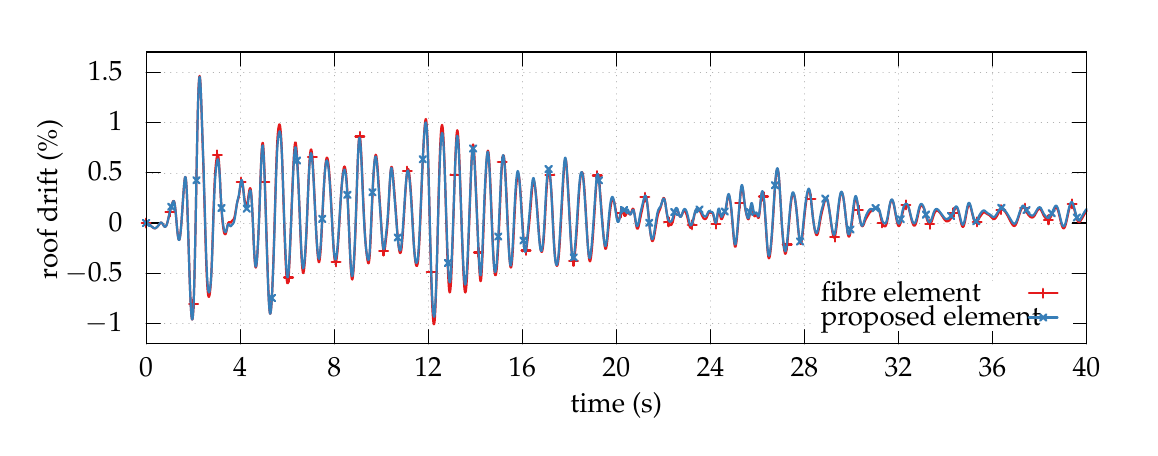
\begin{tikzpicture}[gnuplot]
%% generated with GNUPLOT 5.4p5 (Lua 5.4; terminal rev. Jun 2020, script rev. 115)
%% 06/16/23 03:09:18
\path (0.000,0.000) rectangle (14.000,5.000);
\gpcolor{color=gp lt color axes}
\gpsetlinetype{gp lt axes}
\gpsetdashtype{gp dt axes}
\gpsetlinewidth{0.50}
\draw[gp path] (1.504,1.241)--(9.955,1.241);
\draw[gp path] (13.263,1.241)--(13.447,1.241);
\gpcolor{color=gp lt color border}
\gpsetlinetype{gp lt border}
\gpsetdashtype{gp dt solid}
\gpsetlinewidth{1.00}
\draw[gp path] (1.504,1.241)--(1.684,1.241);
\draw[gp path] (13.447,1.241)--(13.267,1.241);
\node[gp node right] at (1.320,1.241) {$-1$};
\gpcolor{color=gp lt color axes}
\gpsetlinetype{gp lt axes}
\gpsetdashtype{gp dt axes}
\gpsetlinewidth{0.50}
\draw[gp path] (1.504,1.880)--(13.447,1.880);
\gpcolor{color=gp lt color border}
\gpsetlinetype{gp lt border}
\gpsetdashtype{gp dt solid}
\gpsetlinewidth{1.00}
\draw[gp path] (1.504,1.880)--(1.684,1.880);
\draw[gp path] (13.447,1.880)--(13.267,1.880);
\node[gp node right] at (1.320,1.880) {$-0.5$};
\gpcolor{color=gp lt color axes}
\gpsetlinetype{gp lt axes}
\gpsetdashtype{gp dt axes}
\gpsetlinewidth{0.50}
\draw[gp path] (1.504,2.519)--(13.447,2.519);
\gpcolor{color=gp lt color border}
\gpsetlinetype{gp lt border}
\gpsetdashtype{gp dt solid}
\gpsetlinewidth{1.00}
\draw[gp path] (1.504,2.519)--(1.684,2.519);
\draw[gp path] (13.447,2.519)--(13.267,2.519);
\node[gp node right] at (1.320,2.519) {$0$};
\gpcolor{color=gp lt color axes}
\gpsetlinetype{gp lt axes}
\gpsetdashtype{gp dt axes}
\gpsetlinewidth{0.50}
\draw[gp path] (1.504,3.157)--(13.447,3.157);
\gpcolor{color=gp lt color border}
\gpsetlinetype{gp lt border}
\gpsetdashtype{gp dt solid}
\gpsetlinewidth{1.00}
\draw[gp path] (1.504,3.157)--(1.684,3.157);
\draw[gp path] (13.447,3.157)--(13.267,3.157);
\node[gp node right] at (1.320,3.157) {$0.5$};
\gpcolor{color=gp lt color axes}
\gpsetlinetype{gp lt axes}
\gpsetdashtype{gp dt axes}
\gpsetlinewidth{0.50}
\draw[gp path] (1.504,3.796)--(13.447,3.796);
\gpcolor{color=gp lt color border}
\gpsetlinetype{gp lt border}
\gpsetdashtype{gp dt solid}
\gpsetlinewidth{1.00}
\draw[gp path] (1.504,3.796)--(1.684,3.796);
\draw[gp path] (13.447,3.796)--(13.267,3.796);
\node[gp node right] at (1.320,3.796) {$1$};
\gpcolor{color=gp lt color axes}
\gpsetlinetype{gp lt axes}
\gpsetdashtype{gp dt axes}
\gpsetlinewidth{0.50}
\draw[gp path] (1.504,4.435)--(13.447,4.435);
\gpcolor{color=gp lt color border}
\gpsetlinetype{gp lt border}
\gpsetdashtype{gp dt solid}
\gpsetlinewidth{1.00}
\draw[gp path] (1.504,4.435)--(1.684,4.435);
\draw[gp path] (13.447,4.435)--(13.267,4.435);
\node[gp node right] at (1.320,4.435) {$1.5$};
\gpcolor{color=gp lt color axes}
\gpsetlinetype{gp lt axes}
\gpsetdashtype{gp dt axes}
\gpsetlinewidth{0.50}
\draw[gp path] (1.504,0.985)--(1.504,4.691);
\gpcolor{color=gp lt color border}
\gpsetlinetype{gp lt border}
\gpsetdashtype{gp dt solid}
\gpsetlinewidth{1.00}
\draw[gp path] (1.504,0.985)--(1.504,1.165);
\draw[gp path] (1.504,4.691)--(1.504,4.511);
\node[gp node center] at (1.504,0.677) {$0$};
\gpcolor{color=gp lt color axes}
\gpsetlinetype{gp lt axes}
\gpsetdashtype{gp dt axes}
\gpsetlinewidth{0.50}
\draw[gp path] (2.698,0.985)--(2.698,4.691);
\gpcolor{color=gp lt color border}
\gpsetlinetype{gp lt border}
\gpsetdashtype{gp dt solid}
\gpsetlinewidth{1.00}
\draw[gp path] (2.698,0.985)--(2.698,1.165);
\draw[gp path] (2.698,4.691)--(2.698,4.511);
\node[gp node center] at (2.698,0.677) {$4$};
\gpcolor{color=gp lt color axes}
\gpsetlinetype{gp lt axes}
\gpsetdashtype{gp dt axes}
\gpsetlinewidth{0.50}
\draw[gp path] (3.893,0.985)--(3.893,4.691);
\gpcolor{color=gp lt color border}
\gpsetlinetype{gp lt border}
\gpsetdashtype{gp dt solid}
\gpsetlinewidth{1.00}
\draw[gp path] (3.893,0.985)--(3.893,1.165);
\draw[gp path] (3.893,4.691)--(3.893,4.511);
\node[gp node center] at (3.893,0.677) {$8$};
\gpcolor{color=gp lt color axes}
\gpsetlinetype{gp lt axes}
\gpsetdashtype{gp dt axes}
\gpsetlinewidth{0.50}
\draw[gp path] (5.087,0.985)--(5.087,4.691);
\gpcolor{color=gp lt color border}
\gpsetlinetype{gp lt border}
\gpsetdashtype{gp dt solid}
\gpsetlinewidth{1.00}
\draw[gp path] (5.087,0.985)--(5.087,1.165);
\draw[gp path] (5.087,4.691)--(5.087,4.511);
\node[gp node center] at (5.087,0.677) {$12$};
\gpcolor{color=gp lt color axes}
\gpsetlinetype{gp lt axes}
\gpsetdashtype{gp dt axes}
\gpsetlinewidth{0.50}
\draw[gp path] (6.281,0.985)--(6.281,4.691);
\gpcolor{color=gp lt color border}
\gpsetlinetype{gp lt border}
\gpsetdashtype{gp dt solid}
\gpsetlinewidth{1.00}
\draw[gp path] (6.281,0.985)--(6.281,1.165);
\draw[gp path] (6.281,4.691)--(6.281,4.511);
\node[gp node center] at (6.281,0.677) {$16$};
\gpcolor{color=gp lt color axes}
\gpsetlinetype{gp lt axes}
\gpsetdashtype{gp dt axes}
\gpsetlinewidth{0.50}
\draw[gp path] (7.476,0.985)--(7.476,4.691);
\gpcolor{color=gp lt color border}
\gpsetlinetype{gp lt border}
\gpsetdashtype{gp dt solid}
\gpsetlinewidth{1.00}
\draw[gp path] (7.476,0.985)--(7.476,1.165);
\draw[gp path] (7.476,4.691)--(7.476,4.511);
\node[gp node center] at (7.476,0.677) {$20$};
\gpcolor{color=gp lt color axes}
\gpsetlinetype{gp lt axes}
\gpsetdashtype{gp dt axes}
\gpsetlinewidth{0.50}
\draw[gp path] (8.670,0.985)--(8.670,4.691);
\gpcolor{color=gp lt color border}
\gpsetlinetype{gp lt border}
\gpsetdashtype{gp dt solid}
\gpsetlinewidth{1.00}
\draw[gp path] (8.670,0.985)--(8.670,1.165);
\draw[gp path] (8.670,4.691)--(8.670,4.511);
\node[gp node center] at (8.670,0.677) {$24$};
\gpcolor{color=gp lt color axes}
\gpsetlinetype{gp lt axes}
\gpsetdashtype{gp dt axes}
\gpsetlinewidth{0.50}
\draw[gp path] (9.864,0.985)--(9.864,4.691);
\gpcolor{color=gp lt color border}
\gpsetlinetype{gp lt border}
\gpsetdashtype{gp dt solid}
\gpsetlinewidth{1.00}
\draw[gp path] (9.864,0.985)--(9.864,1.165);
\draw[gp path] (9.864,4.691)--(9.864,4.511);
\node[gp node center] at (9.864,0.677) {$28$};
\gpcolor{color=gp lt color axes}
\gpsetlinetype{gp lt axes}
\gpsetdashtype{gp dt axes}
\gpsetlinewidth{0.50}
\draw[gp path] (11.058,0.985)--(11.058,1.165);
\draw[gp path] (11.058,1.781)--(11.058,4.691);
\gpcolor{color=gp lt color border}
\gpsetlinetype{gp lt border}
\gpsetdashtype{gp dt solid}
\gpsetlinewidth{1.00}
\draw[gp path] (11.058,0.985)--(11.058,1.165);
\draw[gp path] (11.058,4.691)--(11.058,4.511);
\node[gp node center] at (11.058,0.677) {$32$};
\gpcolor{color=gp lt color axes}
\gpsetlinetype{gp lt axes}
\gpsetdashtype{gp dt axes}
\gpsetlinewidth{0.50}
\draw[gp path] (12.253,0.985)--(12.253,1.165);
\draw[gp path] (12.253,1.781)--(12.253,4.691);
\gpcolor{color=gp lt color border}
\gpsetlinetype{gp lt border}
\gpsetdashtype{gp dt solid}
\gpsetlinewidth{1.00}
\draw[gp path] (12.253,0.985)--(12.253,1.165);
\draw[gp path] (12.253,4.691)--(12.253,4.511);
\node[gp node center] at (12.253,0.677) {$36$};
\gpcolor{color=gp lt color axes}
\gpsetlinetype{gp lt axes}
\gpsetdashtype{gp dt axes}
\gpsetlinewidth{0.50}
\draw[gp path] (13.447,0.985)--(13.447,4.691);
\gpcolor{color=gp lt color border}
\gpsetlinetype{gp lt border}
\gpsetdashtype{gp dt solid}
\gpsetlinewidth{1.00}
\draw[gp path] (13.447,0.985)--(13.447,1.165);
\draw[gp path] (13.447,4.691)--(13.447,4.511);
\node[gp node center] at (13.447,0.677) {$40$};
\draw[gp path] (1.504,4.691)--(1.504,0.985)--(13.447,0.985)--(13.447,4.691)--cycle;
\node[gp node center,rotate=-270] at (0.292,2.838) {roof drift (\si{\percent})};
\node[gp node center] at (7.475,0.215) {time (\si{\second})};
\gpcolor{rgb color={0.894,0.102,0.110}}
\gpsetlinewidth{2.00}
\draw[gp path] (1.504,2.519)--(1.507,2.518)--(1.510,2.518)--(1.513,2.518)--(1.516,2.517)%
  --(1.519,2.517)--(1.522,2.516)--(1.525,2.515)--(1.528,2.513)--(1.531,2.512)--(1.534,2.510)%
  --(1.537,2.508)--(1.540,2.506)--(1.543,2.503)--(1.546,2.500)--(1.549,2.498)--(1.552,2.495)%
  --(1.555,2.492)--(1.558,2.489)--(1.561,2.486)--(1.564,2.483)--(1.567,2.481)--(1.570,2.478)%
  --(1.573,2.476)--(1.576,2.473)--(1.579,2.471)--(1.582,2.468)--(1.585,2.466)--(1.588,2.464)%
  --(1.591,2.462)--(1.594,2.460)--(1.597,2.458)--(1.600,2.456)--(1.603,2.455)--(1.606,2.454)%
  --(1.609,2.452)--(1.611,2.452)--(1.614,2.452)--(1.617,2.452)--(1.620,2.452)--(1.623,2.454)%
  --(1.626,2.455)--(1.629,2.457)--(1.632,2.459)--(1.635,2.461)--(1.638,2.463)--(1.641,2.466)%
  --(1.644,2.468)--(1.647,2.471)--(1.650,2.474)--(1.653,2.478)--(1.656,2.482)--(1.659,2.486)%
  --(1.662,2.490)--(1.665,2.494)--(1.668,2.499)--(1.671,2.503)--(1.674,2.507)--(1.677,2.511)%
  --(1.680,2.515)--(1.683,2.518)--(1.686,2.521)--(1.689,2.523)--(1.692,2.524)--(1.695,2.525)%
  --(1.698,2.524)--(1.701,2.522)--(1.704,2.520)--(1.707,2.517)--(1.710,2.514)--(1.713,2.510)%
  --(1.716,2.505)--(1.719,2.500)--(1.722,2.495)--(1.725,2.490)--(1.728,2.486)--(1.731,2.481)%
  --(1.734,2.478)--(1.737,2.475)--(1.740,2.473)--(1.743,2.472)--(1.746,2.472)--(1.749,2.473)%
  --(1.752,2.475)--(1.755,2.478)--(1.758,2.482)--(1.761,2.488)--(1.764,2.494)--(1.767,2.502)%
  --(1.770,2.511)--(1.773,2.521)--(1.776,2.531)--(1.779,2.543)--(1.782,2.555)--(1.785,2.569)%
  --(1.788,2.582)--(1.791,2.595)--(1.794,2.608)--(1.797,2.622)--(1.800,2.635)--(1.803,2.648)%
  --(1.806,2.660)--(1.809,2.672)--(1.812,2.684)--(1.815,2.695)--(1.818,2.705)--(1.820,2.716)%
  --(1.823,2.726)--(1.826,2.736)--(1.829,2.746)--(1.832,2.756)--(1.835,2.765)--(1.838,2.773)%
  --(1.841,2.781)--(1.844,2.788)--(1.847,2.793)--(1.850,2.797)--(1.853,2.799)--(1.856,2.798)%
  --(1.859,2.793)--(1.862,2.784)--(1.865,2.772)--(1.868,2.755)--(1.871,2.735)--(1.874,2.711)%
  --(1.877,2.683)--(1.880,2.653)--(1.883,2.620)--(1.886,2.586)--(1.889,2.551)--(1.892,2.516)%
  --(1.895,2.482)--(1.898,2.449)--(1.901,2.418)--(1.904,2.390)--(1.907,2.366)--(1.910,2.345)%
  --(1.913,2.328)--(1.916,2.316)--(1.919,2.308)--(1.922,2.304)--(1.925,2.306)--(1.928,2.312)%
  --(1.931,2.323)--(1.934,2.339)--(1.937,2.359)--(1.940,2.384)--(1.943,2.412)--(1.946,2.444)%
  --(1.949,2.478)--(1.952,2.516)--(1.955,2.555)--(1.958,2.597)--(1.961,2.640)--(1.964,2.684)%
  --(1.967,2.729)--(1.970,2.773)--(1.973,2.817)--(1.976,2.859)--(1.979,2.902)--(1.982,2.941)%
  --(1.985,2.980)--(1.988,3.015)--(1.991,3.047)--(1.994,3.072)--(1.997,3.090)--(2.000,3.101)%
  --(2.003,3.101)--(2.006,3.094)--(2.009,3.076)--(2.012,3.051)--(2.015,3.012)--(2.018,2.966)%
  --(2.021,2.909)--(2.024,2.845)--(2.027,2.771)--(2.029,2.691)--(2.032,2.604)--(2.035,2.513)%
  --(2.038,2.418)--(2.041,2.322)--(2.044,2.225)--(2.047,2.128)--(2.050,2.032)--(2.053,1.940)%
  --(2.056,1.851)--(2.059,1.766)--(2.062,1.684)--(2.065,1.610)--(2.068,1.542)--(2.071,1.482)%
  --(2.074,1.429)--(2.077,1.383)--(2.080,1.347)--(2.083,1.319)--(2.086,1.301)--(2.089,1.294)%
  --(2.092,1.297)--(2.095,1.312)--(2.098,1.336)--(2.101,1.375)--(2.104,1.425)--(2.107,1.493)%
  --(2.110,1.567)--(2.113,1.659)--(2.116,1.762)--(2.119,1.876)--(2.122,2.000)--(2.125,2.132)%
  --(2.128,2.274)--(2.131,2.424)--(2.134,2.579)--(2.137,2.738)--(2.140,2.902)--(2.143,3.065)%
  --(2.146,3.228)--(2.149,3.388)--(2.152,3.544)--(2.155,3.690)--(2.158,3.825)--(2.161,3.949)%
  --(2.164,4.056)--(2.167,4.148)--(2.170,4.230)--(2.173,4.290)--(2.176,4.340)--(2.179,4.372)%
  --(2.182,4.386)--(2.185,4.386)--(2.188,4.368)--(2.191,4.336)--(2.194,4.293)--(2.197,4.233)%
  --(2.200,4.166)--(2.203,4.091)--(2.206,4.009)--(2.209,3.921)--(2.212,3.832)--(2.215,3.740)%
  --(2.218,3.647)--(2.221,3.555)--(2.224,3.466)--(2.227,3.378)--(2.230,3.289)--(2.233,3.200)%
  --(2.236,3.108)--(2.238,3.012)--(2.241,2.913)--(2.244,2.813)--(2.247,2.709)--(2.250,2.604)%
  --(2.253,2.498)--(2.256,2.391)--(2.259,2.287)--(2.262,2.187)--(2.265,2.093)--(2.268,2.007)%
  --(2.271,1.929)--(2.274,1.858)--(2.277,1.798)--(2.280,1.741)--(2.283,1.695)--(2.286,1.659)%
  --(2.289,1.628)--(2.292,1.606)--(2.295,1.592)--(2.298,1.581)--(2.301,1.581)--(2.304,1.585)%
  --(2.307,1.592)--(2.310,1.606)--(2.313,1.624)--(2.316,1.649)--(2.319,1.677)--(2.322,1.709)%
  --(2.325,1.748)--(2.328,1.794)--(2.331,1.844)--(2.334,1.904)--(2.337,1.975)--(2.340,2.050)%
  --(2.343,2.132)--(2.346,2.220)--(2.349,2.313)--(2.352,2.409)--(2.355,2.505)--(2.358,2.601)%
  --(2.361,2.693)--(2.364,2.781)--(2.367,2.864)--(2.370,2.941)--(2.373,3.008)--(2.376,3.069)%
  --(2.379,3.122)--(2.382,3.172)--(2.385,3.211)--(2.388,3.243)--(2.391,3.275)--(2.394,3.299)%
  --(2.397,3.321)--(2.400,3.342)--(2.403,3.360)--(2.406,3.374)--(2.409,3.385)--(2.412,3.388)%
  --(2.415,3.388)--(2.418,3.381)--(2.421,3.370)--(2.424,3.349)--(2.427,3.321)--(2.430,3.285)%
  --(2.433,3.243)--(2.436,3.193)--(2.439,3.140)--(2.442,3.083)--(2.445,3.023)--(2.447,2.962)%
  --(2.450,2.902)--(2.453,2.844)--(2.456,2.790)--(2.459,2.741)--(2.462,2.695)--(2.465,2.652)%
  --(2.468,2.613)--(2.471,2.577)--(2.474,2.545)--(2.477,2.516)--(2.480,2.489)--(2.483,2.465)%
  --(2.486,2.444)--(2.489,2.425)--(2.492,2.408)--(2.495,2.396)--(2.498,2.388)--(2.501,2.383)%
  --(2.504,2.379)--(2.507,2.377)--(2.510,2.377)--(2.513,2.380)--(2.516,2.385)--(2.519,2.394)%
  --(2.522,2.405)--(2.525,2.418)--(2.528,2.433)--(2.531,2.449)--(2.534,2.466)--(2.537,2.482)%
  --(2.540,2.496)--(2.543,2.507)--(2.546,2.516)--(2.549,2.522)--(2.552,2.526)--(2.555,2.529)%
  --(2.558,2.530)--(2.561,2.530)--(2.564,2.529)--(2.567,2.527)--(2.570,2.526)--(2.573,2.525)%
  --(2.576,2.525)--(2.579,2.526)--(2.582,2.529)--(2.585,2.533)--(2.588,2.537)--(2.591,2.541)%
  --(2.594,2.545)--(2.597,2.548)--(2.600,2.551)--(2.603,2.554)--(2.606,2.557)--(2.609,2.559)%
  --(2.612,2.562)--(2.615,2.566)--(2.618,2.571)--(2.621,2.577)--(2.624,2.586)--(2.627,2.596)%
  --(2.630,2.608)--(2.633,2.622)--(2.636,2.637)--(2.639,2.654)--(2.642,2.672)--(2.645,2.690)%
  --(2.648,2.708)--(2.651,2.725)--(2.654,2.742)--(2.656,2.757)--(2.659,2.771)--(2.662,2.784)%
  --(2.665,2.795)--(2.668,2.806)--(2.671,2.816)--(2.674,2.826)--(2.677,2.837)--(2.680,2.850)%
  --(2.683,2.865)--(2.686,2.881)--(2.689,2.902)--(2.692,2.923)--(2.695,2.944)--(2.698,2.966)%
  --(2.701,2.987)--(2.704,3.008)--(2.707,3.023)--(2.710,3.040)--(2.713,3.051)--(2.716,3.058)%
  --(2.719,3.058)--(2.722,3.055)--(2.725,3.047)--(2.728,3.033)--(2.731,3.012)--(2.734,2.991)%
  --(2.737,2.966)--(2.740,2.941)--(2.743,2.913)--(2.746,2.888)--(2.749,2.861)--(2.752,2.837)%
  --(2.755,2.815)--(2.758,2.795)--(2.761,2.778)--(2.764,2.765)--(2.767,2.754)--(2.770,2.747)%
  --(2.773,2.743)--(2.776,2.741)--(2.779,2.743)--(2.782,2.747)--(2.785,2.755)--(2.788,2.764)%
  --(2.791,2.777)--(2.794,2.792)--(2.797,2.811)--(2.800,2.832)--(2.803,2.855)--(2.806,2.877)%
  --(2.809,2.898)--(2.812,2.916)--(2.815,2.934)--(2.818,2.948)--(2.821,2.955)--(2.824,2.962)%
  --(2.827,2.962)--(2.830,2.955)--(2.833,2.941)--(2.836,2.923)--(2.839,2.895)--(2.842,2.858)%
  --(2.845,2.816)--(2.848,2.766)--(2.851,2.712)--(2.854,2.653)--(2.857,2.591)--(2.860,2.526)%
  --(2.863,2.460)--(2.866,2.394)--(2.868,2.328)--(2.871,2.264)--(2.874,2.204)--(2.877,2.146)%
  --(2.880,2.096)--(2.883,2.050)--(2.886,2.014)--(2.889,1.986)--(2.892,1.965)--(2.895,1.954)%
  --(2.898,1.954)--(2.901,1.961)--(2.904,1.975)--(2.907,1.997)--(2.910,2.025)--(2.913,2.061)%
  --(2.916,2.103)--(2.919,2.153)--(2.922,2.204)--(2.925,2.261)--(2.928,2.322)--(2.931,2.385)%
  --(2.934,2.453)--(2.937,2.524)--(2.940,2.599)--(2.943,2.678)--(2.946,2.762)--(2.949,2.850)%
  --(2.952,2.941)--(2.955,3.030)--(2.958,3.115)--(2.961,3.197)--(2.964,3.271)--(2.967,3.339)%
  --(2.970,3.399)--(2.973,3.449)--(2.976,3.491)--(2.979,3.520)--(2.982,3.534)--(2.985,3.537)%
  --(2.988,3.530)--(2.991,3.505)--(2.994,3.466)--(2.997,3.417)--(3.000,3.360)--(3.003,3.289)%
  --(3.006,3.214)--(3.009,3.133)--(3.012,3.044)--(3.015,2.952)--(3.018,2.858)--(3.021,2.761)%
  --(3.024,2.663)--(3.027,2.564)--(3.030,2.465)--(3.033,2.368)--(3.036,2.272)--(3.039,2.178)%
  --(3.042,2.085)--(3.045,1.993)--(3.048,1.904)--(3.051,1.819)--(3.054,1.741)--(3.057,1.667)%
  --(3.060,1.596)--(3.063,1.535)--(3.066,1.486)--(3.069,1.443)--(3.072,1.407)--(3.075,1.386)%
  --(3.077,1.372)--(3.080,1.368)--(3.083,1.375)--(3.086,1.390)--(3.089,1.411)--(3.092,1.439)%
  --(3.095,1.478)--(3.098,1.521)--(3.101,1.574)--(3.104,1.631)--(3.107,1.691)--(3.110,1.759)%
  --(3.113,1.833)--(3.116,1.908)--(3.119,1.990)--(3.122,2.075)--(3.125,2.165)--(3.128,2.260)%
  --(3.131,2.359)--(3.134,2.463)--(3.137,2.568)--(3.140,2.675)--(3.143,2.782)--(3.146,2.888)%
  --(3.149,2.991)--(3.152,3.090)--(3.155,3.182)--(3.158,3.271)--(3.161,3.353)--(3.164,3.427)%
  --(3.167,3.495)--(3.170,3.555)--(3.173,3.605)--(3.176,3.644)--(3.179,3.679)--(3.182,3.708)%
  --(3.185,3.729)--(3.188,3.747)--(3.191,3.757)--(3.194,3.768)--(3.197,3.772)--(3.200,3.768)%
  --(3.203,3.761)--(3.206,3.747)--(3.209,3.725)--(3.212,3.697)--(3.215,3.662)--(3.218,3.619)%
  --(3.221,3.569)--(3.224,3.512)--(3.227,3.445)--(3.230,3.374)--(3.233,3.296)--(3.236,3.211)%
  --(3.239,3.118)--(3.242,3.023)--(3.245,2.927)--(3.248,2.828)--(3.251,2.730)--(3.254,2.634)%
  --(3.257,2.541)--(3.260,2.450)--(3.263,2.363)--(3.266,2.280)--(3.269,2.202)--(3.272,2.128)%
  --(3.275,2.061)--(3.278,1.997)--(3.281,1.940)--(3.284,1.890)--(3.286,1.848)--(3.289,1.812)%
  --(3.292,1.784)--(3.295,1.766)--(3.298,1.755)--(3.301,1.752)--(3.304,1.755)--(3.307,1.770)%
  --(3.310,1.794)--(3.313,1.826)--(3.316,1.865)--(3.319,1.912)--(3.322,1.968)--(3.325,2.029)%
  --(3.328,2.096)--(3.331,2.164)--(3.334,2.237)--(3.337,2.312)--(3.340,2.389)--(3.343,2.466)%
  --(3.346,2.544)--(3.349,2.623)--(3.352,2.701)--(3.355,2.779)--(3.358,2.856)--(3.361,2.934)%
  --(3.364,3.008)--(3.367,3.079)--(3.370,3.150)--(3.373,3.218)--(3.376,3.278)--(3.379,3.339)%
  --(3.382,3.388)--(3.385,3.434)--(3.388,3.473)--(3.391,3.505)--(3.394,3.527)--(3.397,3.541)%
  --(3.400,3.544)--(3.403,3.541)--(3.406,3.530)--(3.409,3.509)--(3.412,3.484)--(3.415,3.449)%
  --(3.418,3.410)--(3.421,3.363)--(3.424,3.314)--(3.427,3.257)--(3.430,3.200)--(3.433,3.140)%
  --(3.436,3.072)--(3.439,3.008)--(3.442,2.937)--(3.445,2.866)--(3.448,2.793)--(3.451,2.718)%
  --(3.454,2.642)--(3.457,2.566)--(3.460,2.490)--(3.463,2.415)--(3.466,2.342)--(3.469,2.271)%
  --(3.472,2.204)--(3.475,2.142)--(3.478,2.085)--(3.481,2.032)--(3.484,1.990)--(3.487,1.954)%
  --(3.490,1.926)--(3.493,1.904)--(3.495,1.890)--(3.498,1.883)--(3.501,1.883)--(3.504,1.894)%
  --(3.507,1.908)--(3.510,1.926)--(3.513,1.954)--(3.516,1.986)--(3.519,2.022)--(3.522,2.061)%
  --(3.525,2.107)--(3.528,2.153)--(3.531,2.207)--(3.534,2.264)--(3.537,2.325)--(3.540,2.389)%
  --(3.543,2.457)--(3.546,2.528)--(3.549,2.602)--(3.552,2.678)--(3.555,2.755)--(3.558,2.833)%
  --(3.561,2.909)--(3.564,2.987)--(3.567,3.058)--(3.570,3.126)--(3.573,3.186)--(3.576,3.243)%
  --(3.579,3.296)--(3.582,3.339)--(3.585,3.378)--(3.588,3.406)--(3.591,3.431)--(3.594,3.445)%
  --(3.597,3.452)--(3.600,3.452)--(3.603,3.449)--(3.606,3.434)--(3.609,3.413)--(3.612,3.388)%
  --(3.615,3.356)--(3.618,3.317)--(3.621,3.275)--(3.624,3.228)--(3.627,3.175)--(3.630,3.122)%
  --(3.633,3.062)--(3.636,3.001)--(3.639,2.937)--(3.642,2.873)--(3.645,2.809)--(3.648,2.743)%
  --(3.651,2.678)--(3.654,2.613)--(3.657,2.549)--(3.660,2.487)--(3.663,2.427)--(3.666,2.370)%
  --(3.669,2.317)--(3.672,2.266)--(3.675,2.220)--(3.678,2.178)--(3.681,2.139)--(3.684,2.107)%
  --(3.687,2.078)--(3.690,2.053)--(3.693,2.039)--(3.696,2.025)--(3.699,2.022)--(3.702,2.022)%
  --(3.704,2.029)--(3.707,2.043)--(3.710,2.064)--(3.713,2.089)--(3.716,2.121)--(3.719,2.156)%
  --(3.722,2.199)--(3.725,2.246)--(3.728,2.297)--(3.731,2.352)--(3.734,2.410)--(3.737,2.470)%
  --(3.740,2.532)--(3.743,2.594)--(3.746,2.657)--(3.749,2.720)--(3.752,2.782)--(3.755,2.842)%
  --(3.758,2.902)--(3.761,2.955)--(3.764,3.008)--(3.767,3.062)--(3.770,3.108)--(3.773,3.150)%
  --(3.776,3.189)--(3.779,3.225)--(3.782,3.257)--(3.785,3.282)--(3.788,3.303)--(3.791,3.321)%
  --(3.794,3.335)--(3.797,3.346)--(3.800,3.349)--(3.803,3.349)--(3.806,3.342)--(3.809,3.335)%
  --(3.812,3.321)--(3.815,3.303)--(3.818,3.282)--(3.821,3.257)--(3.824,3.228)--(3.827,3.197)%
  --(3.830,3.161)--(3.833,3.122)--(3.836,3.083)--(3.839,3.037)--(3.842,2.991)--(3.845,2.941)%
  --(3.848,2.888)--(3.851,2.833)--(3.854,2.777)--(3.857,2.719)--(3.860,2.660)--(3.863,2.601)%
  --(3.866,2.541)--(3.869,2.482)--(3.872,2.423)--(3.875,2.367)--(3.878,2.312)--(3.881,2.261)%
  --(3.884,2.214)--(3.887,2.171)--(3.890,2.132)--(3.893,2.100)--(3.896,2.075)--(3.899,2.050)%
  --(3.902,2.032)--(3.905,2.022)--(3.908,2.014)--(3.911,2.014)--(3.914,2.018)--(3.916,2.025)%
  --(3.919,2.036)--(3.922,2.053)--(3.925,2.075)--(3.928,2.100)--(3.931,2.128)--(3.934,2.156)%
  --(3.937,2.193)--(3.940,2.231)--(3.943,2.272)--(3.946,2.316)--(3.949,2.362)--(3.952,2.411)%
  --(3.955,2.461)--(3.958,2.512)--(3.961,2.564)--(3.964,2.615)--(3.967,2.667)--(3.970,2.718)%
  --(3.973,2.768)--(3.976,2.817)--(3.979,2.863)--(3.982,2.909)--(3.985,2.952)--(3.988,2.991)%
  --(3.991,3.026)--(3.994,3.062)--(3.997,3.094)--(4.000,3.122)--(4.003,3.147)--(4.006,3.172)%
  --(4.009,3.189)--(4.012,3.207)--(4.015,3.221)--(4.018,3.228)--(4.021,3.236)--(4.024,3.236)%
  --(4.027,3.232)--(4.030,3.225)--(4.033,3.214)--(4.036,3.197)--(4.039,3.175)--(4.042,3.150)%
  --(4.045,3.122)--(4.048,3.090)--(4.051,3.051)--(4.054,3.008)--(4.057,2.959)--(4.060,2.905)%
  --(4.063,2.849)--(4.066,2.789)--(4.069,2.724)--(4.072,2.657)--(4.075,2.588)--(4.078,2.516)%
  --(4.081,2.443)--(4.084,2.370)--(4.087,2.297)--(4.090,2.226)--(4.093,2.156)--(4.096,2.093)%
  --(4.099,2.032)--(4.102,1.979)--(4.105,1.929)--(4.108,1.890)--(4.111,1.855)--(4.114,1.830)%
  --(4.117,1.812)--(4.120,1.805)--(4.123,1.801)--(4.125,1.809)--(4.128,1.823)--(4.131,1.844)%
  --(4.134,1.872)--(4.137,1.908)--(4.140,1.951)--(4.143,1.997)--(4.146,2.046)--(4.149,2.103)%
  --(4.152,2.164)--(4.155,2.230)--(4.158,2.300)--(4.161,2.375)--(4.164,2.455)--(4.167,2.538)%
  --(4.170,2.625)--(4.173,2.716)--(4.176,2.810)--(4.179,2.905)--(4.182,3.001)--(4.185,3.097)%
  --(4.188,3.186)--(4.191,3.268)--(4.194,3.346)--(4.197,3.413)--(4.200,3.473)--(4.203,3.527)%
  --(4.206,3.569)--(4.209,3.601)--(4.212,3.619)--(4.215,3.626)--(4.218,3.619)--(4.221,3.605)%
  --(4.224,3.580)--(4.227,3.548)--(4.230,3.509)--(4.233,3.459)--(4.236,3.402)--(4.239,3.342)%
  --(4.242,3.278)--(4.245,3.207)--(4.248,3.136)--(4.251,3.062)--(4.254,2.991)--(4.257,2.916)%
  --(4.260,2.847)--(4.263,2.778)--(4.266,2.712)--(4.269,2.647)--(4.272,2.585)--(4.275,2.525)%
  --(4.278,2.468)--(4.281,2.416)--(4.284,2.368)--(4.287,2.323)--(4.290,2.282)--(4.293,2.245)%
  --(4.296,2.211)--(4.299,2.180)--(4.302,2.149)--(4.305,2.124)--(4.308,2.100)--(4.311,2.078)%
  --(4.314,2.057)--(4.317,2.039)--(4.320,2.025)--(4.323,2.014)--(4.326,2.007)--(4.329,2.007)%
  --(4.332,2.011)--(4.334,2.022)--(4.337,2.039)--(4.340,2.064)--(4.343,2.096)--(4.346,2.139)%
  --(4.349,2.188)--(4.352,2.246)--(4.355,2.308)--(4.358,2.374)--(4.361,2.444)--(4.364,2.516)%
  --(4.367,2.589)--(4.370,2.662)--(4.373,2.734)--(4.376,2.804)--(4.379,2.871)--(4.382,2.934)%
  --(4.385,2.994)--(4.388,3.051)--(4.391,3.104)--(4.394,3.154)--(4.397,3.200)--(4.400,3.239)%
  --(4.403,3.275)--(4.406,3.307)--(4.409,3.331)--(4.412,3.353)--(4.415,3.370)--(4.418,3.381)%
  --(4.421,3.385)--(4.424,3.381)--(4.427,3.374)--(4.430,3.356)--(4.433,3.335)--(4.436,3.310)%
  --(4.439,3.275)--(4.442,3.239)--(4.445,3.200)--(4.448,3.157)--(4.451,3.111)--(4.454,3.065)%
  --(4.457,3.019)--(4.460,2.973)--(4.463,2.923)--(4.466,2.877)--(4.469,2.832)--(4.472,2.787)%
  --(4.475,2.742)--(4.478,2.697)--(4.481,2.651)--(4.484,2.604)--(4.487,2.557)--(4.490,2.508)%
  --(4.493,2.460)--(4.496,2.413)--(4.499,2.367)--(4.502,2.324)--(4.505,2.285)--(4.508,2.251)%
  --(4.511,2.220)--(4.514,2.195)--(4.517,2.176)--(4.520,2.164)--(4.523,2.156)--(4.526,2.156)%
  --(4.529,2.160)--(4.532,2.172)--(4.535,2.188)--(4.538,2.206)--(4.541,2.227)--(4.543,2.250)%
  --(4.546,2.275)--(4.549,2.300)--(4.552,2.326)--(4.555,2.353)--(4.558,2.381)--(4.561,2.411)%
  --(4.564,2.442)--(4.567,2.476)--(4.570,2.513)--(4.573,2.554)--(4.576,2.598)--(4.579,2.646)%
  --(4.582,2.698)--(4.585,2.754)--(4.588,2.811)--(4.591,2.869)--(4.594,2.927)--(4.597,2.984)%
  --(4.600,3.037)--(4.603,3.083)--(4.606,3.126)--(4.609,3.165)--(4.612,3.193)--(4.615,3.214)%
  --(4.618,3.228)--(4.621,3.232)--(4.624,3.232)--(4.627,3.221)--(4.630,3.204)--(4.633,3.182)%
  --(4.636,3.154)--(4.639,3.126)--(4.642,3.094)--(4.645,3.058)--(4.648,3.023)--(4.651,2.987)%
  --(4.654,2.948)--(4.657,2.913)--(4.660,2.873)--(4.663,2.835)--(4.666,2.796)--(4.669,2.757)%
  --(4.672,2.717)--(4.675,2.676)--(4.678,2.634)--(4.681,2.592)--(4.684,2.549)--(4.687,2.507)%
  --(4.690,2.465)--(4.693,2.424)--(4.696,2.385)--(4.699,2.348)--(4.702,2.314)--(4.705,2.281)%
  --(4.708,2.252)--(4.711,2.226)--(4.714,2.203)--(4.717,2.183)--(4.720,2.166)--(4.723,2.153)%
  --(4.726,2.142)--(4.729,2.139)--(4.732,2.139)--(4.735,2.139)--(4.738,2.146)--(4.741,2.156)%
  --(4.744,2.172)--(4.747,2.191)--(4.750,2.214)--(4.752,2.241)--(4.755,2.272)--(4.758,2.307)%
  --(4.761,2.344)--(4.764,2.384)--(4.767,2.426)--(4.770,2.471)--(4.773,2.517)--(4.776,2.564)%
  --(4.779,2.613)--(4.782,2.662)--(4.785,2.712)--(4.788,2.762)--(4.791,2.811)--(4.794,2.860)%
  --(4.797,2.909)--(4.800,2.955)--(4.803,2.998)--(4.806,3.037)--(4.809,3.072)--(4.812,3.108)%
  --(4.815,3.136)--(4.818,3.157)--(4.821,3.179)--(4.824,3.193)--(4.827,3.200)--(4.830,3.204)%
  --(4.833,3.204)--(4.836,3.197)--(4.839,3.186)--(4.842,3.172)--(4.845,3.150)--(4.848,3.129)%
  --(4.851,3.101)--(4.854,3.072)--(4.857,3.040)--(4.860,3.001)--(4.863,2.962)--(4.866,2.920)%
  --(4.869,2.877)--(4.872,2.828)--(4.875,2.778)--(4.878,2.726)--(4.881,2.672)--(4.884,2.616)%
  --(4.887,2.560)--(4.890,2.503)--(4.893,2.446)--(4.896,2.391)--(4.899,2.339)--(4.902,2.288)%
  --(4.905,2.240)--(4.908,2.196)--(4.911,2.156)--(4.914,2.121)--(4.917,2.089)--(4.920,2.061)%
  --(4.923,2.036)--(4.926,2.018)--(4.929,2.000)--(4.932,1.990)--(4.935,1.979)--(4.938,1.975)%
  --(4.941,1.972)--(4.944,1.975)--(4.947,1.982)--(4.950,1.993)--(4.953,2.007)--(4.956,2.025)%
  --(4.959,2.050)--(4.961,2.082)--(4.964,2.117)--(4.967,2.160)--(4.970,2.207)--(4.973,2.260)%
  --(4.976,2.318)--(4.979,2.380)--(4.982,2.446)--(4.985,2.516)--(4.988,2.588)--(4.991,2.663)%
  --(4.994,2.738)--(4.997,2.814)--(5.000,2.891)--(5.003,2.966)--(5.006,3.040)--(5.009,3.115)%
  --(5.012,3.186)--(5.015,3.253)--(5.018,3.321)--(5.021,3.385)--(5.024,3.449)--(5.027,3.505)%
  --(5.030,3.562)--(5.033,3.612)--(5.036,3.662)--(5.039,3.704)--(5.042,3.743)--(5.045,3.779)%
  --(5.048,3.804)--(5.051,3.825)--(5.054,3.835)--(5.057,3.839)--(5.060,3.832)--(5.063,3.814)%
  --(5.066,3.782)--(5.069,3.743)--(5.072,3.694)--(5.075,3.633)--(5.078,3.562)--(5.081,3.481)%
  --(5.084,3.392)--(5.087,3.292)--(5.090,3.186)--(5.093,3.072)--(5.096,2.955)--(5.099,2.836)%
  --(5.102,2.713)--(5.105,2.589)--(5.108,2.466)--(5.111,2.345)--(5.114,2.226)--(5.117,2.110)%
  --(5.120,2.000)--(5.123,1.894)--(5.126,1.794)--(5.129,1.702)--(5.132,1.617)--(5.135,1.542)%
  --(5.138,1.471)--(5.141,1.411)--(5.144,1.361)--(5.147,1.319)--(5.150,1.283)--(5.153,1.258)%
  --(5.156,1.241)--(5.159,1.233)--(5.162,1.237)--(5.165,1.248)--(5.168,1.273)--(5.171,1.304)%
  --(5.173,1.347)--(5.176,1.400)--(5.179,1.461)--(5.182,1.532)--(5.185,1.610)--(5.188,1.699)%
  --(5.191,1.794)--(5.194,1.894)--(5.197,2.004)--(5.200,2.117)--(5.203,2.233)--(5.206,2.352)%
  --(5.209,2.473)--(5.212,2.594)--(5.215,2.714)--(5.218,2.831)--(5.221,2.944)--(5.224,3.055)%
  --(5.227,3.157)--(5.230,3.253)--(5.233,3.342)--(5.236,3.424)--(5.239,3.498)--(5.242,3.562)%
  --(5.245,3.619)--(5.248,3.665)--(5.251,3.701)--(5.254,3.733)--(5.257,3.750)--(5.260,3.761)%
  --(5.263,3.764)--(5.266,3.757)--(5.269,3.740)--(5.272,3.715)--(5.275,3.683)--(5.278,3.640)%
  --(5.281,3.587)--(5.284,3.527)--(5.287,3.456)--(5.290,3.381)--(5.293,3.299)--(5.296,3.211)%
  --(5.299,3.118)--(5.302,3.023)--(5.305,2.923)--(5.308,2.823)--(5.311,2.721)--(5.314,2.618)%
  --(5.317,2.516)--(5.320,2.416)--(5.323,2.318)--(5.326,2.224)--(5.329,2.135)--(5.332,2.050)%
  --(5.335,1.975)--(5.338,1.901)--(5.341,1.837)--(5.344,1.784)--(5.347,1.734)--(5.350,1.695)%
  --(5.353,1.667)--(5.356,1.649)--(5.359,1.638)--(5.362,1.638)--(5.365,1.649)--(5.368,1.670)%
  --(5.371,1.699)--(5.374,1.738)--(5.377,1.780)--(5.380,1.837)--(5.382,1.897)--(5.385,1.965)%
  --(5.388,2.036)--(5.391,2.117)--(5.394,2.199)--(5.397,2.286)--(5.400,2.376)--(5.403,2.467)%
  --(5.406,2.561)--(5.409,2.655)--(5.412,2.750)--(5.415,2.845)--(5.418,2.941)--(5.421,3.033)%
  --(5.424,3.126)--(5.427,3.214)--(5.430,3.299)--(5.433,3.378)--(5.436,3.449)--(5.439,3.512)%
  --(5.442,3.569)--(5.445,3.615)--(5.448,3.651)--(5.451,3.676)--(5.454,3.694)--(5.457,3.697)%
  --(5.460,3.686)--(5.463,3.669)--(5.466,3.640)--(5.469,3.598)--(5.472,3.552)--(5.475,3.495)%
  --(5.478,3.431)--(5.481,3.360)--(5.484,3.285)--(5.487,3.207)--(5.490,3.126)--(5.493,3.040)%
  --(5.496,2.952)--(5.499,2.861)--(5.502,2.770)--(5.505,2.679)--(5.508,2.588)--(5.511,2.498)%
  --(5.514,2.410)--(5.517,2.324)--(5.520,2.241)--(5.523,2.160)--(5.526,2.082)--(5.529,2.007)%
  --(5.532,1.936)--(5.535,1.872)--(5.538,1.816)--(5.541,1.766)--(5.544,1.723)--(5.547,1.688)%
  --(5.550,1.663)--(5.553,1.645)--(5.556,1.638)--(5.559,1.638)--(5.562,1.645)--(5.565,1.659)%
  --(5.568,1.684)--(5.571,1.713)--(5.574,1.752)--(5.577,1.798)--(5.580,1.848)--(5.583,1.901)%
  --(5.586,1.961)--(5.589,2.025)--(5.591,2.093)--(5.594,2.165)--(5.597,2.240)--(5.600,2.318)%
  --(5.603,2.398)--(5.606,2.480)--(5.609,2.563)--(5.612,2.647)--(5.615,2.731)--(5.618,2.815)%
  --(5.621,2.898)--(5.624,2.980)--(5.627,3.062)--(5.630,3.140)--(5.633,3.211)--(5.636,3.282)%
  --(5.639,3.342)--(5.642,3.395)--(5.645,3.438)--(5.648,3.473)--(5.651,3.498)--(5.654,3.512)%
  --(5.657,3.516)--(5.660,3.509)--(5.663,3.491)--(5.666,3.466)--(5.669,3.431)--(5.672,3.388)%
  --(5.675,3.339)--(5.678,3.282)--(5.681,3.221)--(5.684,3.154)--(5.687,3.086)--(5.690,3.015)%
  --(5.693,2.944)--(5.696,2.873)--(5.699,2.801)--(5.702,2.728)--(5.705,2.654)--(5.708,2.580)%
  --(5.711,2.506)--(5.714,2.432)--(5.717,2.359)--(5.720,2.286)--(5.723,2.215)--(5.726,2.146)%
  --(5.729,2.078)--(5.732,2.014)--(5.735,1.958)--(5.738,1.904)--(5.741,1.862)--(5.744,1.826)%
  --(5.747,1.798)--(5.750,1.784)--(5.753,1.780)--(5.756,1.791)--(5.759,1.809)--(5.762,1.841)%
  --(5.765,1.883)--(5.768,1.933)--(5.771,1.993)--(5.774,2.061)--(5.777,2.132)--(5.780,2.205)%
  --(5.783,2.282)--(5.786,2.361)--(5.789,2.439)--(5.792,2.516)--(5.795,2.592)--(5.798,2.666)%
  --(5.800,2.739)--(5.803,2.809)--(5.806,2.877)--(5.809,2.944)--(5.812,3.012)--(5.815,3.072)%
  --(5.818,3.133)--(5.821,3.189)--(5.824,3.243)--(5.827,3.289)--(5.830,3.331)--(5.833,3.367)%
  --(5.836,3.399)--(5.839,3.420)--(5.842,3.431)--(5.845,3.438)--(5.848,3.434)--(5.851,3.420)%
  --(5.854,3.399)--(5.857,3.367)--(5.860,3.331)--(5.863,3.285)--(5.866,3.232)--(5.869,3.175)%
  --(5.872,3.115)--(5.875,3.047)--(5.878,2.976)--(5.881,2.905)--(5.884,2.829)--(5.887,2.754)%
  --(5.890,2.677)--(5.893,2.601)--(5.896,2.524)--(5.899,2.449)--(5.902,2.376)--(5.905,2.305)%
  --(5.908,2.237)--(5.911,2.172)--(5.914,2.114)--(5.917,2.057)--(5.920,2.011)--(5.923,1.968)%
  --(5.926,1.933)--(5.929,1.904)--(5.932,1.883)--(5.935,1.865)--(5.938,1.858)--(5.941,1.855)%
  --(5.944,1.858)--(5.947,1.869)--(5.950,1.883)--(5.953,1.904)--(5.956,1.929)--(5.959,1.961)%
  --(5.962,2.000)--(5.965,2.043)--(5.968,2.089)--(5.971,2.139)--(5.974,2.193)--(5.977,2.252)%
  --(5.980,2.313)--(5.983,2.377)--(5.986,2.444)--(5.989,2.512)--(5.992,2.582)--(5.995,2.653)%
  --(5.998,2.723)--(6.001,2.794)--(6.004,2.863)--(6.007,2.930)--(6.009,2.994)--(6.012,3.058)%
  --(6.015,3.115)--(6.018,3.168)--(6.021,3.218)--(6.024,3.260)--(6.027,3.296)--(6.030,3.324)%
  --(6.033,3.349)--(6.036,3.367)--(6.039,3.378)--(6.042,3.378)--(6.045,3.374)--(6.048,3.363)%
  --(6.051,3.346)--(6.054,3.321)--(6.057,3.289)--(6.060,3.253)--(6.063,3.214)--(6.066,3.168)%
  --(6.069,3.115)--(6.072,3.058)--(6.075,2.998)--(6.078,2.937)--(6.081,2.870)--(6.084,2.803)%
  --(6.087,2.733)--(6.090,2.663)--(6.093,2.593)--(6.096,2.524)--(6.099,2.456)--(6.102,2.390)%
  --(6.105,2.326)--(6.108,2.265)--(6.111,2.207)--(6.114,2.153)--(6.117,2.107)--(6.120,2.064)%
  --(6.123,2.029)--(6.126,2.000)--(6.129,1.975)--(6.132,1.961)--(6.135,1.954)--(6.138,1.954)%
  --(6.141,1.961)--(6.144,1.975)--(6.147,1.993)--(6.150,2.022)--(6.153,2.053)--(6.156,2.093)%
  --(6.159,2.139)--(6.162,2.188)--(6.165,2.242)--(6.168,2.299)--(6.171,2.359)--(6.174,2.421)%
  --(6.177,2.484)--(6.180,2.547)--(6.183,2.609)--(6.186,2.670)--(6.189,2.729)--(6.192,2.785)%
  --(6.195,2.838)--(6.198,2.888)--(6.201,2.934)--(6.204,2.973)--(6.207,3.008)--(6.210,3.044)%
  --(6.213,3.072)--(6.216,3.094)--(6.218,3.115)--(6.221,3.129)--(6.224,3.140)--(6.227,3.143)%
  --(6.230,3.143)--(6.233,3.136)--(6.236,3.126)--(6.239,3.111)--(6.242,3.094)--(6.245,3.069)%
  --(6.248,3.040)--(6.251,3.008)--(6.254,2.973)--(6.257,2.934)--(6.260,2.891)--(6.263,2.847)%
  --(6.266,2.801)--(6.269,2.753)--(6.272,2.705)--(6.275,2.657)--(6.278,2.608)--(6.281,2.560)%
  --(6.284,2.513)--(6.287,2.466)--(6.290,2.422)--(6.293,2.379)--(6.296,2.339)--(6.299,2.302)%
  --(6.302,2.268)--(6.305,2.238)--(6.308,2.212)--(6.311,2.191)--(6.314,2.174)--(6.317,2.164)%
  --(6.320,2.156)--(6.323,2.156)--(6.326,2.160)--(6.329,2.171)--(6.332,2.186)--(6.335,2.204)%
  --(6.338,2.224)--(6.341,2.247)--(6.344,2.272)--(6.347,2.298)--(6.350,2.326)--(6.353,2.354)%
  --(6.356,2.383)--(6.359,2.411)--(6.362,2.440)--(6.365,2.470)--(6.368,2.500)--(6.371,2.532)%
  --(6.374,2.564)--(6.377,2.597)--(6.380,2.632)--(6.383,2.668)--(6.386,2.705)--(6.389,2.743)%
  --(6.392,2.781)--(6.395,2.819)--(6.398,2.856)--(6.401,2.891)--(6.404,2.927)--(6.407,2.955)%
  --(6.410,2.984)--(6.413,3.005)--(6.416,3.026)--(6.419,3.040)--(6.422,3.051)--(6.425,3.055)%
  --(6.428,3.055)--(6.430,3.051)--(6.433,3.044)--(6.436,3.030)--(6.439,3.015)--(6.442,2.994)%
  --(6.445,2.973)--(6.448,2.948)--(6.451,2.923)--(6.454,2.895)--(6.457,2.863)--(6.460,2.830)%
  --(6.463,2.795)--(6.466,2.759)--(6.469,2.721)--(6.472,2.681)--(6.475,2.640)--(6.478,2.599)%
  --(6.481,2.557)--(6.484,2.514)--(6.487,2.472)--(6.490,2.431)--(6.493,2.391)--(6.496,2.353)%
  --(6.499,2.317)--(6.502,2.284)--(6.505,2.254)--(6.508,2.228)--(6.511,2.206)--(6.514,2.187)%
  --(6.517,2.173)--(6.520,2.164)--(6.523,2.156)--(6.526,2.153)--(6.529,2.153)--(6.532,2.156)%
  --(6.535,2.165)--(6.538,2.177)--(6.541,2.194)--(6.544,2.215)--(6.547,2.240)--(6.550,2.270)%
  --(6.553,2.305)--(6.556,2.344)--(6.559,2.388)--(6.562,2.435)--(6.565,2.486)--(6.568,2.540)%
  --(6.571,2.596)--(6.574,2.654)--(6.577,2.712)--(6.580,2.769)--(6.583,2.825)--(6.586,2.877)%
  --(6.589,2.927)--(6.592,2.973)--(6.595,3.015)--(6.598,3.051)--(6.601,3.083)--(6.604,3.108)%
  --(6.607,3.129)--(6.610,3.143)--(6.613,3.154)--(6.616,3.161)--(6.619,3.161)--(6.622,3.157)%
  --(6.625,3.154)--(6.628,3.143)--(6.631,3.129)--(6.634,3.111)--(6.637,3.090)--(6.639,3.065)%
  --(6.642,3.033)--(6.645,3.001)--(6.648,2.959)--(6.651,2.916)--(6.654,2.865)--(6.657,2.811)%
  --(6.660,2.755)--(6.663,2.695)--(6.666,2.633)--(6.669,2.571)--(6.672,2.508)--(6.675,2.447)%
  --(6.678,2.389)--(6.681,2.333)--(6.684,2.280)--(6.687,2.232)--(6.690,2.187)--(6.693,2.149)%
  --(6.696,2.114)--(6.699,2.082)--(6.702,2.053)--(6.705,2.032)--(6.708,2.014)--(6.711,2.000)%
  --(6.714,1.990)--(6.717,1.982)--(6.720,1.975)--(6.723,1.975)--(6.726,1.979)--(6.729,1.986)%
  --(6.732,1.997)--(6.735,2.014)--(6.738,2.032)--(6.741,2.061)--(6.744,2.089)--(6.747,2.121)%
  --(6.750,2.160)--(6.753,2.201)--(6.756,2.246)--(6.759,2.293)--(6.762,2.342)--(6.765,2.394)%
  --(6.768,2.445)--(6.771,2.498)--(6.774,2.552)--(6.777,2.606)--(6.780,2.660)--(6.783,2.715)%
  --(6.786,2.770)--(6.789,2.825)--(6.792,2.881)--(6.795,2.934)--(6.798,2.987)--(6.801,3.040)%
  --(6.804,3.094)--(6.807,3.140)--(6.810,3.186)--(6.813,3.225)--(6.816,3.260)--(6.819,3.289)%
  --(6.822,3.310)--(6.825,3.324)--(6.828,3.331)--(6.831,3.331)--(6.834,3.324)--(6.837,3.310)%
  --(6.840,3.289)--(6.843,3.260)--(6.846,3.228)--(6.848,3.189)--(6.851,3.147)--(6.854,3.104)%
  --(6.857,3.058)--(6.860,3.008)--(6.863,2.959)--(6.866,2.905)--(6.869,2.853)--(6.872,2.799)%
  --(6.875,2.744)--(6.878,2.689)--(6.881,2.632)--(6.884,2.576)--(6.887,2.520)--(6.890,2.464)%
  --(6.893,2.409)--(6.896,2.356)--(6.899,2.305)--(6.902,2.256)--(6.905,2.211)--(6.908,2.170)%
  --(6.911,2.132)--(6.914,2.100)--(6.917,2.075)--(6.920,2.053)--(6.923,2.043)--(6.926,2.032)%
  --(6.929,2.032)--(6.932,2.032)--(6.935,2.043)--(6.938,2.053)--(6.941,2.071)--(6.944,2.089)%
  --(6.947,2.110)--(6.950,2.139)--(6.953,2.166)--(6.956,2.198)--(6.959,2.232)--(6.962,2.269)%
  --(6.965,2.308)--(6.968,2.350)--(6.971,2.393)--(6.974,2.439)--(6.977,2.487)--(6.980,2.536)%
  --(6.983,2.587)--(6.986,2.638)--(6.989,2.689)--(6.992,2.740)--(6.995,2.789)--(6.998,2.837)%
  --(7.001,2.881)--(7.004,2.923)--(7.007,2.962)--(7.010,3.001)--(7.013,3.033)--(7.016,3.062)%
  --(7.019,3.086)--(7.022,3.108)--(7.025,3.126)--(7.028,3.140)--(7.031,3.150)--(7.034,3.157)%
  --(7.037,3.161)--(7.040,3.165)--(7.043,3.161)--(7.046,3.154)--(7.049,3.147)--(7.052,3.133)%
  --(7.055,3.115)--(7.057,3.094)--(7.060,3.069)--(7.063,3.037)--(7.066,3.005)--(7.069,2.966)%
  --(7.072,2.927)--(7.075,2.881)--(7.078,2.836)--(7.081,2.787)--(7.084,2.737)--(7.087,2.686)%
  --(7.090,2.634)--(7.093,2.580)--(7.096,2.527)--(7.099,2.474)--(7.102,2.423)--(7.105,2.372)%
  --(7.108,2.323)--(7.111,2.276)--(7.114,2.232)--(7.117,2.192)--(7.120,2.156)--(7.123,2.121)%
  --(7.126,2.096)--(7.129,2.071)--(7.132,2.053)--(7.135,2.043)--(7.138,2.036)--(7.141,2.032)%
  --(7.144,2.036)--(7.147,2.046)--(7.150,2.061)--(7.153,2.078)--(7.156,2.100)--(7.159,2.124)%
  --(7.162,2.153)--(7.165,2.185)--(7.168,2.219)--(7.171,2.254)--(7.174,2.292)--(7.177,2.331)%
  --(7.180,2.373)--(7.183,2.415)--(7.186,2.459)--(7.189,2.504)--(7.192,2.550)--(7.195,2.598)%
  --(7.198,2.646)--(7.201,2.696)--(7.204,2.745)--(7.207,2.795)--(7.210,2.844)--(7.213,2.891)%
  --(7.216,2.937)--(7.219,2.980)--(7.222,3.019)--(7.225,3.051)--(7.228,3.083)--(7.231,3.104)%
  --(7.234,3.122)--(7.237,3.133)--(7.240,3.140)--(7.243,3.140)--(7.246,3.133)--(7.249,3.122)%
  --(7.252,3.104)--(7.255,3.083)--(7.258,3.058)--(7.261,3.030)--(7.264,2.998)--(7.266,2.962)%
  --(7.269,2.923)--(7.272,2.888)--(7.275,2.847)--(7.278,2.807)--(7.281,2.767)--(7.284,2.727)%
  --(7.287,2.686)--(7.290,2.646)--(7.293,2.605)--(7.296,2.566)--(7.299,2.528)--(7.302,2.490)%
  --(7.305,2.453)--(7.308,2.418)--(7.311,2.384)--(7.314,2.351)--(7.317,2.320)--(7.320,2.291)%
  --(7.323,2.266)--(7.326,2.243)--(7.329,2.224)--(7.332,2.209)--(7.335,2.198)--(7.338,2.192)%
  --(7.341,2.190)--(7.344,2.194)--(7.347,2.202)--(7.350,2.215)--(7.353,2.232)--(7.356,2.253)%
  --(7.359,2.278)--(7.362,2.306)--(7.365,2.337)--(7.368,2.369)--(7.371,2.403)--(7.374,2.437)%
  --(7.377,2.471)--(7.380,2.505)--(7.383,2.538)--(7.386,2.569)--(7.389,2.600)--(7.392,2.629)%
  --(7.395,2.656)--(7.398,2.682)--(7.401,2.705)--(7.404,2.727)--(7.407,2.746)--(7.410,2.763)%
  --(7.413,2.779)--(7.416,2.792)--(7.419,2.803)--(7.422,2.811)--(7.425,2.818)--(7.428,2.822)%
  --(7.431,2.823)--(7.434,2.822)--(7.437,2.819)--(7.440,2.813)--(7.443,2.805)--(7.446,2.796)%
  --(7.449,2.785)--(7.452,2.772)--(7.455,2.757)--(7.458,2.742)--(7.461,2.725)--(7.464,2.708)%
  --(7.467,2.691)--(7.470,2.673)--(7.473,2.655)--(7.476,2.638)--(7.478,2.621)--(7.481,2.606)%
  --(7.484,2.592)--(7.487,2.580)--(7.490,2.569)--(7.493,2.561)--(7.496,2.555)--(7.499,2.551)%
  --(7.502,2.550)--(7.505,2.552)--(7.508,2.556)--(7.511,2.562)--(7.514,2.570)--(7.517,2.580)%
  --(7.520,2.591)--(7.523,2.603)--(7.526,2.615)--(7.529,2.626)--(7.532,2.637)--(7.535,2.647)%
  --(7.538,2.654)--(7.541,2.661)--(7.544,2.664)--(7.547,2.666)--(7.550,2.666)--(7.553,2.664)%
  --(7.556,2.660)--(7.559,2.654)--(7.562,2.648)--(7.565,2.641)--(7.568,2.633)--(7.571,2.626)%
  --(7.574,2.620)--(7.577,2.615)--(7.580,2.612)--(7.583,2.610)--(7.586,2.610)--(7.589,2.611)%
  --(7.592,2.614)--(7.595,2.618)--(7.598,2.623)--(7.601,2.629)--(7.604,2.635)--(7.607,2.640)%
  --(7.610,2.645)--(7.613,2.650)--(7.616,2.653)--(7.619,2.654)--(7.622,2.654)--(7.625,2.653)%
  --(7.628,2.650)--(7.631,2.647)--(7.634,2.643)--(7.637,2.639)--(7.640,2.635)--(7.643,2.632)%
  --(7.646,2.630)--(7.649,2.629)--(7.652,2.630)--(7.655,2.632)--(7.658,2.637)--(7.661,2.643)%
  --(7.664,2.650)--(7.667,2.658)--(7.670,2.667)--(7.673,2.675)--(7.676,2.684)--(7.679,2.691)%
  --(7.682,2.696)--(7.685,2.700)--(7.687,2.701)--(7.690,2.699)--(7.693,2.694)--(7.696,2.686)%
  --(7.699,2.675)--(7.702,2.661)--(7.705,2.644)--(7.708,2.625)--(7.711,2.605)--(7.714,2.584)%
  --(7.717,2.562)--(7.720,2.540)--(7.723,2.520)--(7.726,2.501)--(7.729,2.485)--(7.732,2.471)%
  --(7.735,2.460)--(7.738,2.452)--(7.741,2.448)--(7.744,2.446)--(7.747,2.448)--(7.750,2.452)%
  --(7.753,2.458)--(7.756,2.467)--(7.759,2.478)--(7.762,2.491)--(7.765,2.505)--(7.768,2.519)%
  --(7.771,2.535)--(7.774,2.550)--(7.777,2.565)--(7.780,2.580)--(7.783,2.595)--(7.786,2.609)%
  --(7.789,2.623)--(7.792,2.637)--(7.795,2.651)--(7.798,2.664)--(7.801,2.678)--(7.804,2.692)%
  --(7.807,2.707)--(7.810,2.721)--(7.813,2.736)--(7.816,2.752)--(7.819,2.768)--(7.822,2.783)%
  --(7.825,2.798)--(7.828,2.812)--(7.831,2.826)--(7.834,2.837)--(7.837,2.846)--(7.840,2.853)%
  --(7.843,2.858)--(7.846,2.859)--(7.849,2.858)--(7.852,2.853)--(7.855,2.845)--(7.858,2.834)%
  --(7.861,2.820)--(7.864,2.802)--(7.867,2.782)--(7.870,2.759)--(7.873,2.734)--(7.876,2.707)%
  --(7.879,2.679)--(7.882,2.650)--(7.885,2.620)--(7.888,2.590)--(7.891,2.560)--(7.894,2.530)%
  --(7.896,2.502)--(7.899,2.473)--(7.902,2.447)--(7.905,2.422)--(7.908,2.398)--(7.911,2.376)%
  --(7.914,2.356)--(7.917,2.339)--(7.920,2.324)--(7.923,2.311)--(7.926,2.301)--(7.929,2.295)%
  --(7.932,2.290)--(7.935,2.289)--(7.938,2.291)--(7.941,2.295)--(7.944,2.302)--(7.947,2.310)%
  --(7.950,2.322)--(7.953,2.334)--(7.956,2.349)--(7.959,2.364)--(7.962,2.381)--(7.965,2.399)%
  --(7.968,2.417)--(7.971,2.435)--(7.974,2.455)--(7.977,2.474)--(7.980,2.493)--(7.983,2.512)%
  --(7.986,2.531)--(7.989,2.549)--(7.992,2.566)--(7.995,2.582)--(7.998,2.597)--(8.001,2.611)%
  --(8.004,2.624)--(8.007,2.635)--(8.010,2.645)--(8.013,2.654)--(8.016,2.662)--(8.019,2.669)%
  --(8.022,2.676)--(8.025,2.683)--(8.028,2.690)--(8.031,2.697)--(8.034,2.705)--(8.037,2.713)%
  --(8.040,2.723)--(8.043,2.733)--(8.046,2.744)--(8.049,2.755)--(8.052,2.767)--(8.055,2.779)%
  --(8.058,2.790)--(8.061,2.801)--(8.064,2.811)--(8.067,2.820)--(8.070,2.828)--(8.073,2.833)%
  --(8.076,2.836)--(8.079,2.837)--(8.082,2.834)--(8.085,2.829)--(8.088,2.821)--(8.091,2.810)%
  --(8.094,2.796)--(8.097,2.780)--(8.100,2.763)--(8.103,2.743)--(8.105,2.723)--(8.108,2.702)%
  --(8.111,2.681)--(8.114,2.659)--(8.117,2.639)--(8.120,2.620)--(8.123,2.602)--(8.126,2.585)%
  --(8.129,2.570)--(8.132,2.557)--(8.135,2.545)--(8.138,2.535)--(8.141,2.526)--(8.144,2.519)%
  --(8.147,2.512)--(8.150,2.507)--(8.153,2.503)--(8.156,2.499)--(8.159,2.497)--(8.162,2.495)%
  --(8.165,2.494)--(8.168,2.494)--(8.171,2.495)--(8.174,2.497)--(8.177,2.500)--(8.180,2.504)%
  --(8.183,2.510)--(8.186,2.517)--(8.189,2.525)--(8.192,2.534)--(8.195,2.545)--(8.198,2.557)%
  --(8.201,2.569)--(8.204,2.581)--(8.207,2.594)--(8.210,2.606)--(8.213,2.619)--(8.216,2.631)%
  --(8.219,2.642)--(8.222,2.653)--(8.225,2.663)--(8.228,2.671)--(8.231,2.678)--(8.234,2.684)%
  --(8.237,2.688)--(8.240,2.690)--(8.243,2.691)--(8.246,2.690)--(8.249,2.687)--(8.252,2.683)%
  --(8.255,2.676)--(8.258,2.669)--(8.261,2.662)--(8.264,2.653)--(8.267,2.644)--(8.270,2.635)%
  --(8.273,2.626)--(8.276,2.619)--(8.279,2.612)--(8.282,2.606)--(8.285,2.602)--(8.288,2.600)%
  --(8.291,2.599)--(8.294,2.600)--(8.297,2.602)--(8.300,2.606)--(8.303,2.611)--(8.306,2.616)%
  --(8.309,2.623)--(8.312,2.630)--(8.314,2.637)--(8.317,2.644)--(8.320,2.651)--(8.323,2.657)%
  --(8.326,2.663)--(8.329,2.667)--(8.332,2.670)--(8.335,2.672)--(8.338,2.673)--(8.341,2.673)%
  --(8.344,2.672)--(8.347,2.669)--(8.350,2.665)--(8.353,2.661)--(8.356,2.656)--(8.359,2.650)%
  --(8.362,2.642)--(8.365,2.634)--(8.368,2.626)--(8.371,2.616)--(8.374,2.606)--(8.377,2.595)%
  --(8.380,2.583)--(8.383,2.571)--(8.386,2.559)--(8.389,2.546)--(8.392,2.533)--(8.395,2.520)%
  --(8.398,2.508)--(8.401,2.496)--(8.404,2.486)--(8.407,2.477)--(8.410,2.470)--(8.413,2.464)%
  --(8.416,2.460)--(8.419,2.459)--(8.422,2.459)--(8.425,2.460)--(8.428,2.464)--(8.431,2.470)%
  --(8.434,2.478)--(8.437,2.487)--(8.440,2.497)--(8.443,2.508)--(8.446,2.521)--(8.449,2.534)%
  --(8.452,2.548)--(8.455,2.562)--(8.458,2.576)--(8.461,2.591)--(8.464,2.605)--(8.467,2.619)%
  --(8.470,2.632)--(8.473,2.644)--(8.476,2.654)--(8.479,2.664)--(8.482,2.672)--(8.485,2.679)%
  --(8.488,2.685)--(8.491,2.689)--(8.494,2.691)--(8.497,2.692)--(8.500,2.693)--(8.503,2.692)%
  --(8.506,2.691)--(8.509,2.690)--(8.512,2.687)--(8.515,2.685)--(8.518,2.683)--(8.521,2.681)%
  --(8.523,2.679)--(8.526,2.677)--(8.529,2.675)--(8.532,2.673)--(8.535,2.671)--(8.538,2.668)%
  --(8.541,2.664)--(8.544,2.660)--(8.547,2.654)--(8.550,2.648)--(8.553,2.641)--(8.556,2.634)%
  --(8.559,2.627)--(8.562,2.620)--(8.565,2.613)--(8.568,2.606)--(8.571,2.600)--(8.574,2.594)%
  --(8.577,2.589)--(8.580,2.585)--(8.583,2.580)--(8.586,2.577)--(8.589,2.575)--(8.592,2.573)%
  --(8.595,2.571)--(8.598,2.570)--(8.601,2.570)--(8.604,2.570)--(8.607,2.570)--(8.610,2.571)%
  --(8.613,2.574)--(8.616,2.577)--(8.619,2.581)--(8.622,2.587)--(8.625,2.593)--(8.628,2.600)%
  --(8.631,2.608)--(8.634,2.615)--(8.637,2.623)--(8.640,2.630)--(8.643,2.637)--(8.646,2.642)%
  --(8.649,2.647)--(8.652,2.651)--(8.655,2.654)--(8.658,2.655)--(8.661,2.656)--(8.664,2.655)%
  --(8.667,2.654)--(8.670,2.653)--(8.673,2.652)--(8.676,2.650)--(8.679,2.649)--(8.682,2.648)%
  --(8.685,2.648)--(8.688,2.647)--(8.691,2.647)--(8.694,2.645)--(8.697,2.643)--(8.700,2.639)%
  --(8.703,2.633)--(8.706,2.625)--(8.709,2.615)--(8.712,2.604)--(8.715,2.591)--(8.718,2.576)%
  --(8.721,2.561)--(8.724,2.546)--(8.727,2.532)--(8.730,2.520)--(8.733,2.510)--(8.735,2.504)%
  --(8.738,2.502)--(8.741,2.505)--(8.744,2.513)--(8.747,2.524)--(8.750,2.540)--(8.753,2.558)%
  --(8.756,2.577)--(8.759,2.598)--(8.762,2.618)--(8.765,2.636)--(8.768,2.652)--(8.771,2.664)%
  --(8.774,2.671)--(8.777,2.673)--(8.780,2.672)--(8.783,2.665)--(8.786,2.656)--(8.789,2.643)%
  --(8.792,2.630)--(8.795,2.615)--(8.798,2.601)--(8.801,2.589)--(8.804,2.579)--(8.807,2.572)%
  --(8.810,2.569)--(8.813,2.568)--(8.816,2.570)--(8.819,2.575)--(8.822,2.581)--(8.825,2.588)%
  --(8.828,2.597)--(8.831,2.604)--(8.834,2.612)--(8.837,2.619)--(8.840,2.626)--(8.843,2.631)%
  --(8.846,2.637)--(8.849,2.642)--(8.852,2.648)--(8.855,2.654)--(8.858,2.662)--(8.861,2.672)%
  --(8.864,2.683)--(8.867,2.697)--(8.870,2.713)--(8.873,2.732)--(8.876,2.752)--(8.879,2.772)%
  --(8.882,2.793)--(8.885,2.813)--(8.888,2.831)--(8.891,2.847)--(8.894,2.860)--(8.897,2.869)%
  --(8.900,2.873)--(8.903,2.873)--(8.906,2.871)--(8.909,2.863)--(8.912,2.853)--(8.915,2.838)%
  --(8.918,2.822)--(8.921,2.803)--(8.924,2.782)--(8.927,2.760)--(8.930,2.736)--(8.933,2.711)%
  --(8.936,2.685)--(8.939,2.657)--(8.942,2.627)--(8.944,2.596)--(8.947,2.563)--(8.950,2.528)%
  --(8.953,2.492)--(8.956,2.456)--(8.959,2.419)--(8.962,2.383)--(8.965,2.348)--(8.968,2.317)%
  --(8.971,2.288)--(8.974,2.263)--(8.977,2.243)--(8.980,2.229)--(8.983,2.220)--(8.986,2.217)%
  --(8.989,2.219)--(8.992,2.227)--(8.995,2.240)--(8.998,2.258)--(9.001,2.279)--(9.004,2.305)%
  --(9.007,2.333)--(9.010,2.364)--(9.013,2.397)--(9.016,2.432)--(9.019,2.468)--(9.022,2.504)%
  --(9.025,2.541)--(9.028,2.579)--(9.031,2.617)--(9.034,2.655)--(9.037,2.694)--(9.040,2.732)%
  --(9.043,2.769)--(9.046,2.806)--(9.049,2.840)--(9.052,2.872)--(9.055,2.902)--(9.058,2.927)%
  --(9.061,2.948)--(9.064,2.966)--(9.067,2.976)--(9.070,2.984)--(9.073,2.980)--(9.076,2.976)%
  --(9.079,2.966)--(9.082,2.948)--(9.085,2.930)--(9.088,2.905)--(9.091,2.881)--(9.094,2.855)%
  --(9.097,2.828)--(9.100,2.803)--(9.103,2.778)--(9.106,2.754)--(9.109,2.732)--(9.112,2.712)%
  --(9.115,2.694)--(9.118,2.677)--(9.121,2.662)--(9.124,2.647)--(9.127,2.634)--(9.130,2.622)%
  --(9.133,2.610)--(9.136,2.599)--(9.139,2.590)--(9.142,2.581)--(9.145,2.574)--(9.148,2.569)%
  --(9.151,2.566)--(9.153,2.567)--(9.156,2.570)--(9.159,2.577)--(9.162,2.587)--(9.165,2.600)%
  --(9.168,2.616)--(9.171,2.635)--(9.174,2.654)--(9.177,2.675)--(9.180,2.694)--(9.183,2.712)%
  --(9.186,2.726)--(9.189,2.737)--(9.192,2.743)--(9.195,2.744)--(9.198,2.740)--(9.201,2.732)%
  --(9.204,2.720)--(9.207,2.705)--(9.210,2.688)--(9.213,2.670)--(9.216,2.653)--(9.219,2.638)%
  --(9.222,2.625)--(9.225,2.615)--(9.228,2.609)--(9.231,2.605)--(9.234,2.605)--(9.237,2.608)%
  --(9.240,2.612)--(9.243,2.616)--(9.246,2.621)--(9.249,2.624)--(9.252,2.626)--(9.255,2.625)%
  --(9.258,2.623)--(9.261,2.618)--(9.264,2.612)--(9.267,2.604)--(9.270,2.597)--(9.273,2.590)%
  --(9.276,2.585)--(9.279,2.584)--(9.282,2.586)--(9.285,2.593)--(9.288,2.605)--(9.291,2.622)%
  --(9.294,2.643)--(9.297,2.669)--(9.300,2.697)--(9.303,2.727)--(9.306,2.758)--(9.309,2.789)%
  --(9.312,2.818)--(9.315,2.845)--(9.318,2.868)--(9.321,2.888)--(9.324,2.902)--(9.327,2.909)%
  --(9.330,2.913)--(9.333,2.909)--(9.336,2.905)--(9.339,2.891)--(9.342,2.877)--(9.345,2.855)%
  --(9.348,2.831)--(9.351,2.804)--(9.354,2.773)--(9.357,2.740)--(9.360,2.703)--(9.362,2.665)%
  --(9.365,2.624)--(9.368,2.581)--(9.371,2.536)--(9.374,2.490)--(9.377,2.443)--(9.380,2.396)%
  --(9.383,2.350)--(9.386,2.305)--(9.389,2.262)--(9.392,2.222)--(9.395,2.186)--(9.398,2.153)%
  --(9.401,2.128)--(9.404,2.107)--(9.407,2.089)--(9.410,2.078)--(9.413,2.071)--(9.416,2.071)%
  --(9.419,2.078)--(9.422,2.085)--(9.425,2.100)--(9.428,2.117)--(9.431,2.139)--(9.434,2.164)%
  --(9.437,2.191)--(9.440,2.221)--(9.443,2.253)--(9.446,2.288)--(9.449,2.325)--(9.452,2.365)%
  --(9.455,2.407)--(9.458,2.451)--(9.461,2.497)--(9.464,2.544)--(9.467,2.592)--(9.470,2.641)%
  --(9.473,2.691)--(9.476,2.741)--(9.479,2.790)--(9.482,2.838)--(9.485,2.884)--(9.488,2.930)%
  --(9.491,2.973)--(9.494,3.012)--(9.497,3.051)--(9.500,3.083)--(9.503,3.115)--(9.506,3.140)%
  --(9.509,3.161)--(9.512,3.179)--(9.515,3.193)--(9.518,3.200)--(9.521,3.204)--(9.524,3.204)%
  --(9.527,3.197)--(9.530,3.182)--(9.533,3.165)--(9.536,3.143)--(9.539,3.115)--(9.542,3.083)%
  --(9.545,3.044)--(9.548,3.001)--(9.551,2.959)--(9.554,2.913)--(9.557,2.861)--(9.560,2.811)%
  --(9.563,2.760)--(9.566,2.708)--(9.569,2.658)--(9.571,2.608)--(9.574,2.560)--(9.577,2.514)%
  --(9.580,2.470)--(9.583,2.428)--(9.586,2.389)--(9.589,2.352)--(9.592,2.318)--(9.595,2.286)%
  --(9.598,2.256)--(9.601,2.229)--(9.604,2.205)--(9.607,2.184)--(9.610,2.166)--(9.613,2.153)%
  --(9.616,2.139)--(9.619,2.132)--(9.622,2.128)--(9.625,2.132)--(9.628,2.135)--(9.631,2.146)%
  --(9.634,2.156)--(9.637,2.174)--(9.640,2.195)--(9.643,2.219)--(9.646,2.246)--(9.649,2.275)%
  --(9.652,2.307)--(9.655,2.340)--(9.658,2.375)--(9.661,2.411)--(9.664,2.447)--(9.667,2.484)%
  --(9.670,2.520)--(9.673,2.556)--(9.676,2.592)--(9.679,2.626)--(9.682,2.659)--(9.685,2.691)%
  --(9.688,2.721)--(9.691,2.750)--(9.694,2.776)--(9.697,2.799)--(9.700,2.821)--(9.703,2.839)%
  --(9.706,2.855)--(9.709,2.869)--(9.712,2.881)--(9.715,2.888)--(9.718,2.891)--(9.721,2.895)%
  --(9.724,2.895)--(9.727,2.891)--(9.730,2.884)--(9.733,2.877)--(9.736,2.867)--(9.739,2.855)%
  --(9.742,2.840)--(9.745,2.825)--(9.748,2.806)--(9.751,2.787)--(9.754,2.765)--(9.757,2.742)%
  --(9.760,2.717)--(9.763,2.690)--(9.766,2.662)--(9.769,2.632)--(9.772,2.602)--(9.775,2.570)%
  --(9.778,2.538)--(9.780,2.505)--(9.783,2.473)--(9.786,2.441)--(9.789,2.411)--(9.792,2.382)%
  --(9.795,2.355)--(9.798,2.330)--(9.801,2.308)--(9.804,2.290)--(9.807,2.275)--(9.810,2.264)%
  --(9.813,2.257)--(9.816,2.254)--(9.819,2.255)--(9.822,2.260)--(9.825,2.269)--(9.828,2.282)%
  --(9.831,2.298)--(9.834,2.318)--(9.837,2.340)--(9.840,2.364)--(9.843,2.391)--(9.846,2.419)%
  --(9.849,2.448)--(9.852,2.478)--(9.855,2.508)--(9.858,2.538)--(9.861,2.568)--(9.864,2.598)%
  --(9.867,2.627)--(9.870,2.655)--(9.873,2.682)--(9.876,2.708)--(9.879,2.733)--(9.882,2.757)%
  --(9.885,2.779)--(9.888,2.801)--(9.891,2.821)--(9.894,2.840)--(9.897,2.858)--(9.900,2.873)%
  --(9.903,2.888)--(9.906,2.902)--(9.909,2.916)--(9.912,2.923)--(9.915,2.930)--(9.918,2.937)%
  --(9.921,2.941)--(9.924,2.937)--(9.927,2.934)--(9.930,2.927)--(9.933,2.916)--(9.936,2.905)%
  --(9.939,2.888)--(9.942,2.867)--(9.945,2.844)--(9.948,2.820)--(9.951,2.793)--(9.954,2.765)%
  --(9.957,2.736)--(9.960,2.707)--(9.963,2.679)--(9.966,2.650)--(9.969,2.623)--(9.972,2.596)%
  --(9.975,2.571)--(9.978,2.548)--(9.981,2.525)--(9.984,2.505)--(9.987,2.485)--(9.990,2.467)%
  --(9.992,2.451)--(9.995,2.436)--(9.998,2.422)--(10.001,2.410)--(10.004,2.399)--(10.007,2.389)%
  --(10.010,2.380)--(10.013,2.374)--(10.016,2.369)--(10.019,2.367)--(10.022,2.366)--(10.025,2.368)%
  --(10.028,2.371)--(10.031,2.377)--(10.034,2.385)--(10.037,2.395)--(10.040,2.407)--(10.043,2.421)%
  --(10.046,2.436)--(10.049,2.452)--(10.052,2.470)--(10.055,2.488)--(10.058,2.506)--(10.061,2.524)%
  --(10.064,2.542)--(10.067,2.559)--(10.070,2.576)--(10.073,2.592)--(10.076,2.607)--(10.079,2.621)%
  --(10.082,2.635)--(10.085,2.648)--(10.088,2.661)--(10.091,2.673)--(10.094,2.685)--(10.097,2.697)%
  --(10.100,2.709)--(10.103,2.721)--(10.106,2.733)--(10.109,2.745)--(10.112,2.757)--(10.115,2.769)%
  --(10.118,2.781)--(10.121,2.792)--(10.124,2.802)--(10.127,2.812)--(10.130,2.820)--(10.133,2.826)%
  --(10.136,2.831)--(10.139,2.834)--(10.142,2.836)--(10.145,2.834)--(10.148,2.832)--(10.151,2.827)%
  --(10.154,2.820)--(10.157,2.811)--(10.160,2.800)--(10.163,2.787)--(10.166,2.772)--(10.169,2.756)%
  --(10.172,2.739)--(10.175,2.721)--(10.178,2.702)--(10.181,2.682)--(10.184,2.662)--(10.187,2.641)%
  --(10.190,2.619)--(10.193,2.598)--(10.196,2.576)--(10.199,2.554)--(10.201,2.533)--(10.204,2.512)%
  --(10.207,2.490)--(10.210,2.470)--(10.213,2.450)--(10.216,2.430)--(10.219,2.412)--(10.222,2.394)%
  --(10.225,2.379)--(10.228,2.364)--(10.231,2.353)--(10.234,2.343)--(10.237,2.336)--(10.240,2.333)%
  --(10.243,2.331)--(10.246,2.334)--(10.249,2.339)--(10.252,2.348)--(10.255,2.359)--(10.258,2.374)%
  --(10.261,2.391)--(10.264,2.410)--(10.267,2.432)--(10.270,2.455)--(10.273,2.480)--(10.276,2.506)%
  --(10.279,2.534)--(10.282,2.561)--(10.285,2.590)--(10.288,2.618)--(10.291,2.647)--(10.294,2.674)%
  --(10.297,2.702)--(10.300,2.728)--(10.303,2.754)--(10.306,2.777)--(10.309,2.800)--(10.312,2.820)%
  --(10.315,2.839)--(10.318,2.855)--(10.321,2.870)--(10.324,2.881)--(10.327,2.891)--(10.330,2.898)%
  --(10.333,2.905)--(10.336,2.905)--(10.339,2.905)--(10.342,2.902)--(10.345,2.898)--(10.348,2.891)%
  --(10.351,2.881)--(10.354,2.867)--(10.357,2.853)--(10.360,2.836)--(10.363,2.818)--(10.366,2.797)%
  --(10.369,2.775)--(10.372,2.752)--(10.375,2.727)--(10.378,2.701)--(10.381,2.674)--(10.384,2.647)%
  --(10.387,2.619)--(10.390,2.590)--(10.393,2.561)--(10.396,2.534)--(10.399,2.507)--(10.402,2.481)%
  --(10.405,2.456)--(10.408,2.433)--(10.410,2.413)--(10.413,2.395)--(10.416,2.379)--(10.419,2.367)%
  --(10.422,2.357)--(10.425,2.351)--(10.428,2.347)--(10.431,2.346)--(10.434,2.348)--(10.437,2.353)%
  --(10.440,2.361)--(10.443,2.371)--(10.446,2.383)--(10.449,2.397)--(10.452,2.413)--(10.455,2.431)%
  --(10.458,2.451)--(10.461,2.472)--(10.464,2.494)--(10.467,2.517)--(10.470,2.542)--(10.473,2.566)%
  --(10.476,2.592)--(10.479,2.618)--(10.482,2.643)--(10.485,2.668)--(10.488,2.693)--(10.491,2.717)%
  --(10.494,2.739)--(10.497,2.760)--(10.500,2.779)--(10.503,2.795)--(10.506,2.810)--(10.509,2.821)%
  --(10.512,2.829)--(10.515,2.834)--(10.518,2.836)--(10.521,2.834)--(10.524,2.829)--(10.527,2.822)%
  --(10.530,2.811)--(10.533,2.798)--(10.536,2.783)--(10.539,2.765)--(10.542,2.747)--(10.545,2.727)%
  --(10.548,2.706)--(10.551,2.686)--(10.554,2.665)--(10.557,2.645)--(10.560,2.624)--(10.563,2.605)%
  --(10.566,2.587)--(10.569,2.570)--(10.572,2.553)--(10.575,2.539)--(10.578,2.525)--(10.581,2.513)%
  --(10.584,2.503)--(10.587,2.495)--(10.590,2.488)--(10.593,2.483)--(10.596,2.480)--(10.599,2.479)%
  --(10.602,2.479)--(10.605,2.481)--(10.608,2.484)--(10.611,2.488)--(10.614,2.494)--(10.617,2.500)%
  --(10.619,2.507)--(10.622,2.515)--(10.625,2.523)--(10.628,2.531)--(10.631,2.539)--(10.634,2.546)%
  --(10.637,2.553)--(10.640,2.560)--(10.643,2.566)--(10.646,2.572)--(10.649,2.578)--(10.652,2.583)%
  --(10.655,2.589)--(10.658,2.594)--(10.661,2.599)--(10.664,2.604)--(10.667,2.609)--(10.670,2.614)%
  --(10.673,2.619)--(10.676,2.625)--(10.679,2.630)--(10.682,2.635)--(10.685,2.640)--(10.688,2.645)%
  --(10.691,2.649)--(10.694,2.653)--(10.697,2.657)--(10.700,2.660)--(10.703,2.663)--(10.706,2.665)%
  --(10.709,2.668)--(10.712,2.669)--(10.715,2.671)--(10.718,2.673)--(10.721,2.674)--(10.724,2.676)%
  --(10.727,2.678)--(10.730,2.680)--(10.733,2.682)--(10.736,2.684)--(10.739,2.687)--(10.742,2.690)%
  --(10.745,2.693)--(10.748,2.696)--(10.751,2.698)--(10.754,2.701)--(10.757,2.703)--(10.760,2.705)%
  --(10.763,2.706)--(10.766,2.707)--(10.769,2.707)--(10.772,2.707)--(10.775,2.707)--(10.778,2.707)%
  --(10.781,2.706)--(10.784,2.706)--(10.787,2.705)--(10.790,2.704)--(10.793,2.703)--(10.796,2.701)%
  --(10.799,2.699)--(10.802,2.696)--(10.805,2.692)--(10.808,2.687)--(10.811,2.681)--(10.814,2.674)%
  --(10.817,2.665)--(10.820,2.654)--(10.823,2.643)--(10.826,2.631)--(10.828,2.618)--(10.831,2.604)%
  --(10.834,2.591)--(10.837,2.577)--(10.840,2.564)--(10.843,2.552)--(10.846,2.540)--(10.849,2.529)%
  --(10.852,2.520)--(10.855,2.511)--(10.858,2.504)--(10.861,2.498)--(10.864,2.492)--(10.867,2.488)%
  --(10.870,2.484)--(10.873,2.482)--(10.876,2.479)--(10.879,2.478)--(10.882,2.477)--(10.885,2.477)%
  --(10.888,2.477)--(10.891,2.478)--(10.894,2.481)--(10.897,2.485)--(10.900,2.490)--(10.903,2.496)%
  --(10.906,2.505)--(10.909,2.514)--(10.912,2.526)--(10.915,2.539)--(10.918,2.554)--(10.921,2.571)%
  --(10.924,2.589)--(10.927,2.608)--(10.930,2.627)--(10.933,2.647)--(10.936,2.666)--(10.939,2.685)%
  --(10.942,2.704)--(10.945,2.721)--(10.948,2.738)--(10.951,2.752)--(10.954,2.766)--(10.957,2.778)%
  --(10.960,2.788)--(10.963,2.796)--(10.966,2.803)--(10.969,2.807)--(10.972,2.810)--(10.975,2.811)%
  --(10.978,2.810)--(10.981,2.807)--(10.984,2.803)--(10.987,2.796)--(10.990,2.788)--(10.993,2.778)%
  --(10.996,2.767)--(10.999,2.755)--(11.002,2.741)--(11.005,2.726)--(11.008,2.710)--(11.011,2.694)%
  --(11.014,2.676)--(11.017,2.659)--(11.020,2.642)--(11.023,2.625)--(11.026,2.608)--(11.029,2.591)%
  --(11.032,2.576)--(11.035,2.561)--(11.037,2.547)--(11.040,2.534)--(11.043,2.522)--(11.046,2.512)%
  --(11.049,2.503)--(11.052,2.495)--(11.055,2.489)--(11.058,2.485)--(11.061,2.482)--(11.064,2.480)%
  --(11.067,2.481)--(11.070,2.483)--(11.073,2.487)--(11.076,2.492)--(11.079,2.500)--(11.082,2.509)%
  --(11.085,2.520)--(11.088,2.533)--(11.091,2.546)--(11.094,2.560)--(11.097,2.575)--(11.100,2.590)%
  --(11.103,2.605)--(11.106,2.620)--(11.109,2.635)--(11.112,2.649)--(11.115,2.662)--(11.118,2.675)%
  --(11.121,2.686)--(11.124,2.696)--(11.127,2.705)--(11.130,2.713)--(11.133,2.721)--(11.136,2.727)%
  --(11.139,2.732)--(11.142,2.737)--(11.145,2.741)--(11.148,2.744)--(11.151,2.746)--(11.154,2.749)%
  --(11.157,2.750)--(11.160,2.751)--(11.163,2.751)--(11.166,2.750)--(11.169,2.748)--(11.172,2.746)%
  --(11.175,2.742)--(11.178,2.737)--(11.181,2.731)--(11.184,2.724)--(11.187,2.715)--(11.190,2.706)%
  --(11.193,2.695)--(11.196,2.684)--(11.199,2.672)--(11.202,2.659)--(11.205,2.646)--(11.208,2.632)%
  --(11.211,2.619)--(11.214,2.606)--(11.217,2.593)--(11.220,2.580)--(11.223,2.568)--(11.226,2.557)%
  --(11.229,2.546)--(11.232,2.536)--(11.235,2.526)--(11.238,2.518)--(11.241,2.510)--(11.244,2.504)%
  --(11.247,2.498)--(11.249,2.494)--(11.252,2.490)--(11.255,2.488)--(11.258,2.486)--(11.261,2.486)%
  --(11.264,2.487)--(11.267,2.489)--(11.270,2.492)--(11.273,2.497)--(11.276,2.502)--(11.279,2.509)%
  --(11.282,2.518)--(11.285,2.527)--(11.288,2.538)--(11.291,2.549)--(11.294,2.561)--(11.297,2.575)%
  --(11.300,2.588)--(11.303,2.602)--(11.306,2.616)--(11.309,2.630)--(11.312,2.644)--(11.315,2.658)%
  --(11.318,2.670)--(11.321,2.683)--(11.324,2.694)--(11.327,2.704)--(11.330,2.713)--(11.333,2.720)%
  --(11.336,2.727)--(11.339,2.732)--(11.342,2.736)--(11.345,2.740)--(11.348,2.742)--(11.351,2.743)%
  --(11.354,2.743)--(11.357,2.742)--(11.360,2.740)--(11.363,2.738)--(11.366,2.734)--(11.369,2.730)%
  --(11.372,2.725)--(11.375,2.720)--(11.378,2.713)--(11.381,2.706)--(11.384,2.698)--(11.387,2.690)%
  --(11.390,2.681)--(11.393,2.671)--(11.396,2.660)--(11.399,2.650)--(11.402,2.638)--(11.405,2.627)%
  --(11.408,2.615)--(11.411,2.604)--(11.414,2.593)--(11.417,2.582)--(11.420,2.571)--(11.423,2.561)%
  --(11.426,2.552)--(11.429,2.544)--(11.432,2.536)--(11.435,2.529)--(11.438,2.522)--(11.441,2.517)%
  --(11.444,2.512)--(11.447,2.509)--(11.450,2.506)--(11.453,2.504)--(11.456,2.503)--(11.458,2.503)%
  --(11.461,2.505)--(11.464,2.507)--(11.467,2.510)--(11.470,2.515)--(11.473,2.520)--(11.476,2.527)%
  --(11.479,2.534)--(11.482,2.542)--(11.485,2.550)--(11.488,2.560)--(11.491,2.569)--(11.494,2.579)%
  --(11.497,2.588)--(11.500,2.598)--(11.503,2.608)--(11.506,2.617)--(11.509,2.625)--(11.512,2.634)%
  --(11.515,2.641)--(11.518,2.647)--(11.521,2.653)--(11.524,2.658)--(11.527,2.663)--(11.530,2.666)%
  --(11.533,2.669)--(11.536,2.672)--(11.539,2.674)--(11.542,2.675)--(11.545,2.675)--(11.548,2.676)%
  --(11.551,2.676)--(11.554,2.675)--(11.557,2.674)--(11.560,2.673)--(11.563,2.671)--(11.566,2.669)%
  --(11.569,2.666)--(11.572,2.663)--(11.575,2.661)--(11.578,2.657)--(11.581,2.654)--(11.584,2.650)%
  --(11.587,2.647)--(11.590,2.643)--(11.593,2.639)--(11.596,2.635)--(11.599,2.631)--(11.602,2.627)%
  --(11.605,2.623)--(11.608,2.618)--(11.611,2.614)--(11.614,2.609)--(11.617,2.604)--(11.620,2.600)%
  --(11.623,2.595)--(11.626,2.590)--(11.629,2.585)--(11.632,2.581)--(11.635,2.576)--(11.638,2.571)%
  --(11.641,2.567)--(11.644,2.563)--(11.647,2.559)--(11.650,2.555)--(11.653,2.552)--(11.656,2.549)%
  --(11.659,2.546)--(11.662,2.545)--(11.665,2.543)--(11.667,2.542)--(11.670,2.541)--(11.673,2.541)%
  --(11.676,2.541)--(11.679,2.541)--(11.682,2.541)--(11.685,2.542)--(11.688,2.543)--(11.691,2.544)%
  --(11.694,2.545)--(11.697,2.547)--(11.700,2.549)--(11.703,2.551)--(11.706,2.554)--(11.709,2.557)%
  --(11.712,2.560)--(11.715,2.564)--(11.718,2.568)--(11.721,2.572)--(11.724,2.576)--(11.727,2.581)%
  --(11.730,2.587)--(11.733,2.593)--(11.736,2.599)--(11.739,2.605)--(11.742,2.612)--(11.745,2.619)%
  --(11.748,2.627)--(11.751,2.635)--(11.754,2.643)--(11.757,2.651)--(11.760,2.659)--(11.763,2.667)%
  --(11.766,2.675)--(11.769,2.683)--(11.772,2.690)--(11.775,2.697)--(11.778,2.703)--(11.781,2.708)%
  --(11.784,2.713)--(11.787,2.716)--(11.790,2.717)--(11.793,2.718)--(11.796,2.717)--(11.799,2.715)%
  --(11.802,2.712)--(11.805,2.707)--(11.808,2.702)--(11.811,2.695)--(11.814,2.687)--(11.817,2.678)%
  --(11.820,2.667)--(11.823,2.656)--(11.826,2.644)--(11.829,2.632)--(11.832,2.619)--(11.835,2.605)%
  --(11.838,2.591)--(11.841,2.577)--(11.844,2.564)--(11.847,2.550)--(11.850,2.537)--(11.853,2.525)%
  --(11.856,2.513)--(11.859,2.503)--(11.862,2.493)--(11.865,2.485)--(11.868,2.479)--(11.871,2.474)%
  --(11.874,2.471)--(11.876,2.470)--(11.879,2.470)--(11.882,2.473)--(11.885,2.477)--(11.888,2.483)%
  --(11.891,2.491)--(11.894,2.501)--(11.897,2.512)--(11.900,2.524)--(11.903,2.538)--(11.906,2.552)%
  --(11.909,2.568)--(11.912,2.584)--(11.915,2.601)--(11.918,2.618)--(11.921,2.634)--(11.924,2.651)%
  --(11.927,2.667)--(11.930,2.682)--(11.933,2.696)--(11.936,2.709)--(11.939,2.721)--(11.942,2.731)%
  --(11.945,2.740)--(11.948,2.746)--(11.951,2.751)--(11.954,2.753)--(11.957,2.754)--(11.960,2.753)%
  --(11.963,2.750)--(11.966,2.745)--(11.969,2.739)--(11.972,2.731)--(11.975,2.722)--(11.978,2.711)%
  --(11.981,2.700)--(11.984,2.689)--(11.987,2.676)--(11.990,2.664)--(11.993,2.652)--(11.996,2.639)%
  --(11.999,2.627)--(12.002,2.615)--(12.005,2.603)--(12.008,2.592)--(12.011,2.581)--(12.014,2.571)%
  --(12.017,2.562)--(12.020,2.553)--(12.023,2.546)--(12.026,2.539)--(12.029,2.533)--(12.032,2.528)%
  --(12.035,2.525)--(12.038,2.522)--(12.041,2.521)--(12.044,2.521)--(12.047,2.522)--(12.050,2.523)%
  --(12.053,2.526)--(12.056,2.530)--(12.059,2.534)--(12.062,2.539)--(12.065,2.544)--(12.068,2.550)%
  --(12.071,2.556)--(12.074,2.562)--(12.077,2.568)--(12.080,2.573)--(12.083,2.579)--(12.085,2.584)%
  --(12.088,2.589)--(12.091,2.594)--(12.094,2.598)--(12.097,2.603)--(12.100,2.607)--(12.103,2.611)%
  --(12.106,2.615)--(12.109,2.620)--(12.112,2.624)--(12.115,2.628)--(12.118,2.632)--(12.121,2.635)%
  --(12.124,2.639)--(12.127,2.642)--(12.130,2.646)--(12.133,2.648)--(12.136,2.650)--(12.139,2.652)%
  --(12.142,2.653)--(12.145,2.654)--(12.148,2.654)--(12.151,2.654)--(12.154,2.653)--(12.157,2.652)%
  --(12.160,2.651)--(12.163,2.649)--(12.166,2.647)--(12.169,2.645)--(12.172,2.643)--(12.175,2.641)%
  --(12.178,2.639)--(12.181,2.637)--(12.184,2.635)--(12.187,2.633)--(12.190,2.631)--(12.193,2.630)%
  --(12.196,2.628)--(12.199,2.627)--(12.202,2.625)--(12.205,2.624)--(12.208,2.622)--(12.211,2.620)%
  --(12.214,2.618)--(12.217,2.615)--(12.220,2.613)--(12.223,2.610)--(12.226,2.607)--(12.229,2.604)%
  --(12.232,2.601)--(12.235,2.597)--(12.238,2.594)--(12.241,2.591)--(12.244,2.587)--(12.247,2.584)%
  --(12.250,2.581)--(12.253,2.579)--(12.256,2.576)--(12.259,2.574)--(12.262,2.572)--(12.265,2.571)%
  --(12.268,2.570)--(12.271,2.570)--(12.274,2.570)--(12.277,2.571)--(12.280,2.572)--(12.283,2.574)%
  --(12.286,2.577)--(12.289,2.579)--(12.292,2.582)--(12.295,2.586)--(12.297,2.590)--(12.300,2.594)%
  --(12.303,2.598)--(12.306,2.603)--(12.309,2.608)--(12.312,2.613)--(12.315,2.618)--(12.318,2.624)%
  --(12.321,2.629)--(12.324,2.635)--(12.327,2.641)--(12.330,2.646)--(12.333,2.652)--(12.336,2.657)%
  --(12.339,2.662)--(12.342,2.667)--(12.345,2.672)--(12.348,2.676)--(12.351,2.680)--(12.354,2.683)%
  --(12.357,2.686)--(12.360,2.689)--(12.363,2.691)--(12.366,2.693)--(12.369,2.694)--(12.372,2.695)%
  --(12.375,2.695)--(12.378,2.695)--(12.381,2.695)--(12.384,2.693)--(12.387,2.692)--(12.390,2.690)%
  --(12.393,2.687)--(12.396,2.684)--(12.399,2.681)--(12.402,2.678)--(12.405,2.674)--(12.408,2.670)%
  --(12.411,2.666)--(12.414,2.662)--(12.417,2.658)--(12.420,2.653)--(12.423,2.649)--(12.426,2.644)%
  --(12.429,2.639)--(12.432,2.634)--(12.435,2.629)--(12.438,2.624)--(12.441,2.619)--(12.444,2.614)%
  --(12.447,2.608)--(12.450,2.602)--(12.453,2.597)--(12.456,2.591)--(12.459,2.585)--(12.462,2.579)%
  --(12.465,2.573)--(12.468,2.567)--(12.471,2.561)--(12.474,2.555)--(12.477,2.549)--(12.480,2.544)%
  --(12.483,2.538)--(12.486,2.533)--(12.489,2.527)--(12.492,2.522)--(12.495,2.517)--(12.498,2.512)%
  --(12.501,2.507)--(12.504,2.503)--(12.506,2.499)--(12.509,2.495)--(12.512,2.492)--(12.515,2.489)%
  --(12.518,2.486)--(12.521,2.484)--(12.524,2.483)--(12.527,2.482)--(12.530,2.482)--(12.533,2.483)%
  --(12.536,2.484)--(12.539,2.486)--(12.542,2.489)--(12.545,2.493)--(12.548,2.498)--(12.551,2.503)%
  --(12.554,2.509)--(12.557,2.516)--(12.560,2.523)--(12.563,2.531)--(12.566,2.539)--(12.569,2.547)%
  --(12.572,2.557)--(12.575,2.566)--(12.578,2.575)--(12.581,2.585)--(12.584,2.594)--(12.587,2.604)%
  --(12.590,2.613)--(12.593,2.623)--(12.596,2.632)--(12.599,2.642)--(12.602,2.651)--(12.605,2.659)%
  --(12.608,2.668)--(12.611,2.676)--(12.614,2.683)--(12.617,2.690)--(12.620,2.697)--(12.623,2.703)%
  --(12.626,2.708)--(12.629,2.712)--(12.632,2.716)--(12.635,2.719)--(12.638,2.721)--(12.641,2.722)%
  --(12.644,2.722)--(12.647,2.722)--(12.650,2.720)--(12.653,2.718)--(12.656,2.715)--(12.659,2.711)%
  --(12.662,2.707)--(12.665,2.702)--(12.668,2.697)--(12.671,2.692)--(12.674,2.686)--(12.677,2.680)%
  --(12.680,2.674)--(12.683,2.668)--(12.686,2.662)--(12.689,2.656)--(12.692,2.650)--(12.695,2.645)%
  --(12.698,2.639)--(12.701,2.634)--(12.704,2.630)--(12.707,2.625)--(12.710,2.621)--(12.713,2.618)%
  --(12.715,2.614)--(12.718,2.611)--(12.721,2.608)--(12.724,2.605)--(12.727,2.603)--(12.730,2.600)%
  --(12.733,2.598)--(12.736,2.596)--(12.739,2.594)--(12.742,2.593)--(12.745,2.592)--(12.748,2.591)%
  --(12.751,2.590)--(12.754,2.590)--(12.757,2.590)--(12.760,2.590)--(12.763,2.591)--(12.766,2.592)%
  --(12.769,2.594)--(12.772,2.596)--(12.775,2.599)--(12.778,2.602)--(12.781,2.605)--(12.784,2.609)%
  --(12.787,2.614)--(12.790,2.618)--(12.793,2.623)--(12.796,2.629)--(12.799,2.634)--(12.802,2.639)%
  --(12.805,2.645)--(12.808,2.650)--(12.811,2.656)--(12.814,2.661)--(12.817,2.666)--(12.820,2.672)%
  --(12.823,2.676)--(12.826,2.681)--(12.829,2.685)--(12.832,2.689)--(12.835,2.692)--(12.838,2.695)%
  --(12.841,2.697)--(12.844,2.698)--(12.847,2.700)--(12.850,2.700)--(12.853,2.700)--(12.856,2.699)%
  --(12.859,2.697)--(12.862,2.694)--(12.865,2.691)--(12.868,2.687)--(12.871,2.682)--(12.874,2.677)%
  --(12.877,2.671)--(12.880,2.665)--(12.883,2.658)--(12.886,2.652)--(12.889,2.645)--(12.892,2.638)%
  --(12.895,2.632)--(12.898,2.625)--(12.901,2.619)--(12.904,2.614)--(12.907,2.609)--(12.910,2.604)%
  --(12.913,2.600)--(12.916,2.596)--(12.919,2.592)--(12.922,2.588)--(12.924,2.585)--(12.927,2.582)%
  --(12.930,2.580)--(12.933,2.577)--(12.936,2.574)--(12.939,2.571)--(12.942,2.569)--(12.945,2.566)%
  --(12.948,2.564)--(12.951,2.563)--(12.954,2.561)--(12.957,2.561)--(12.960,2.561)--(12.963,2.561)%
  --(12.966,2.562)--(12.969,2.564)--(12.972,2.566)--(12.975,2.569)--(12.978,2.573)--(12.981,2.577)%
  --(12.984,2.581)--(12.987,2.586)--(12.990,2.592)--(12.993,2.597)--(12.996,2.603)--(12.999,2.609)%
  --(13.002,2.615)--(13.005,2.621)--(13.008,2.628)--(13.011,2.634)--(13.014,2.641)--(13.017,2.648)%
  --(13.020,2.654)--(13.023,2.661)--(13.026,2.668)--(13.029,2.675)--(13.032,2.682)--(13.035,2.688)%
  --(13.038,2.694)--(13.041,2.700)--(13.044,2.706)--(13.047,2.710)--(13.050,2.714)--(13.053,2.717)%
  --(13.056,2.719)--(13.059,2.719)--(13.062,2.719)--(13.065,2.718)--(13.068,2.715)--(13.071,2.711)%
  --(13.074,2.706)--(13.077,2.700)--(13.080,2.693)--(13.083,2.685)--(13.086,2.676)--(13.089,2.666)%
  --(13.092,2.656)--(13.095,2.645)--(13.098,2.632)--(13.101,2.620)--(13.104,2.608)--(13.107,2.595)%
  --(13.110,2.582)--(13.113,2.569)--(13.116,2.556)--(13.119,2.544)--(13.122,2.531)--(13.125,2.520)%
  --(13.128,2.509)--(13.131,2.498)--(13.133,2.489)--(13.136,2.481)--(13.139,2.473)--(13.142,2.467)%
  --(13.145,2.461)--(13.148,2.457)--(13.151,2.454)--(13.154,2.452)--(13.157,2.452)--(13.160,2.453)%
  --(13.163,2.456)--(13.166,2.459)--(13.169,2.464)--(13.172,2.470)--(13.175,2.477)--(13.178,2.486)%
  --(13.181,2.495)--(13.184,2.506)--(13.187,2.517)--(13.190,2.529)--(13.193,2.542)--(13.196,2.555)%
  --(13.199,2.569)--(13.202,2.583)--(13.205,2.597)--(13.208,2.612)--(13.211,2.626)--(13.214,2.640)%
  --(13.217,2.654)--(13.220,2.667)--(13.223,2.680)--(13.226,2.692)--(13.229,2.704)--(13.232,2.715)%
  --(13.235,2.725)--(13.238,2.734)--(13.241,2.743)--(13.244,2.749)--(13.247,2.755)--(13.250,2.760)%
  --(13.253,2.763)--(13.256,2.765)--(13.259,2.765)--(13.262,2.765)--(13.265,2.762)--(13.268,2.759)%
  --(13.271,2.754)--(13.274,2.748)--(13.277,2.741)--(13.280,2.733)--(13.283,2.724)--(13.286,2.714)%
  --(13.289,2.703)--(13.292,2.693)--(13.295,2.681)--(13.298,2.670)--(13.301,2.658)--(13.304,2.646)%
  --(13.307,2.635)--(13.310,2.623)--(13.313,2.612)--(13.316,2.602)--(13.319,2.591)--(13.322,2.581)%
  --(13.325,2.572)--(13.328,2.564)--(13.331,2.556)--(13.334,2.550)--(13.337,2.544)--(13.340,2.539)%
  --(13.342,2.536)--(13.345,2.533)--(13.348,2.531)--(13.351,2.531)--(13.354,2.531)--(13.357,2.532)%
  --(13.360,2.534)--(13.363,2.537)--(13.366,2.540)--(13.369,2.544)--(13.372,2.548)--(13.375,2.552)%
  --(13.378,2.557)--(13.381,2.562)--(13.384,2.567)--(13.387,2.572)--(13.390,2.577)--(13.393,2.582)%
  --(13.396,2.588)--(13.399,2.593)--(13.402,2.598)--(13.405,2.603)--(13.408,2.609)--(13.411,2.614)%
  --(13.414,2.619)--(13.417,2.625)--(13.420,2.630)--(13.423,2.636)--(13.426,2.641)--(13.429,2.646)%
  --(13.432,2.652)--(13.435,2.656)--(13.438,2.661)--(13.441,2.665)--(13.444,2.669)--(13.447,2.672);
\gpsetpointsize{4.00}
\gp3point{gp mark 1}{}{(1.504,2.519)}
\gp3point{gp mark 1}{}{(1.806,2.660)}
\gp3point{gp mark 1}{}{(2.107,1.493)}
\gp3point{gp mark 1}{}{(2.409,3.385)}
\gp3point{gp mark 1}{}{(2.710,3.040)}
\gp3point{gp mark 1}{}{(3.012,3.044)}
\gp3point{gp mark 1}{}{(3.313,1.826)}
\gp3point{gp mark 1}{}{(3.615,3.356)}
\gp3point{gp mark 1}{}{(3.916,2.025)}
\gp3point{gp mark 1}{}{(4.218,3.619)}
\gp3point{gp mark 1}{}{(4.520,2.164)}
\gp3point{gp mark 1}{}{(4.821,3.179)}
\gp3point{gp mark 1}{}{(5.123,1.894)}
\gp3point{gp mark 1}{}{(5.424,3.126)}
\gp3point{gp mark 1}{}{(5.726,2.146)}
\gp3point{gp mark 1}{}{(6.027,3.296)}
\gp3point{gp mark 1}{}{(6.329,2.171)}
\gp3point{gp mark 1}{}{(6.631,3.129)}
\gp3point{gp mark 1}{}{(6.932,2.032)}
\gp3point{gp mark 1}{}{(7.234,3.122)}
\gp3point{gp mark 1}{}{(7.535,2.647)}
\gp3point{gp mark 1}{}{(7.837,2.846)}
\gp3point{gp mark 1}{}{(8.138,2.535)}
\gp3point{gp mark 1}{}{(8.440,2.497)}
\gp3point{gp mark 1}{}{(8.741,2.505)}
\gp3point{gp mark 1}{}{(9.043,2.769)}
\gp3point{gp mark 1}{}{(9.345,2.855)}
\gp3point{gp mark 1}{}{(9.646,2.246)}
\gp3point{gp mark 1}{}{(9.948,2.820)}
\gp3point{gp mark 1}{}{(10.249,2.339)}
\gp3point{gp mark 1}{}{(10.551,2.686)}
\gp3point{gp mark 1}{}{(10.852,2.520)}
\gp3point{gp mark 1}{}{(11.154,2.749)}
\gp3point{gp mark 1}{}{(11.456,2.503)}
\gp3point{gp mark 1}{}{(11.757,2.651)}
\gp3point{gp mark 1}{}{(12.059,2.534)}
\gp3point{gp mark 1}{}{(12.360,2.689)}
\gp3point{gp mark 1}{}{(12.662,2.707)}
\gp3point{gp mark 1}{}{(12.963,2.561)}
\gp3point{gp mark 1}{}{(13.265,2.762)}
\gpcolor{rgb color={0.216,0.494,0.722}}
\draw[gp path] (1.504,2.519)--(1.507,2.518)--(1.510,2.518)--(1.513,2.518)--(1.516,2.517)%
  --(1.519,2.517)--(1.522,2.516)--(1.525,2.515)--(1.528,2.513)--(1.531,2.512)--(1.534,2.510)%
  --(1.537,2.508)--(1.540,2.506)--(1.543,2.503)--(1.546,2.501)--(1.549,2.498)--(1.552,2.495)%
  --(1.555,2.492)--(1.558,2.489)--(1.561,2.486)--(1.564,2.483)--(1.567,2.481)--(1.570,2.478)%
  --(1.573,2.476)--(1.576,2.473)--(1.579,2.471)--(1.582,2.469)--(1.585,2.467)--(1.588,2.465)%
  --(1.591,2.462)--(1.594,2.461)--(1.597,2.459)--(1.600,2.457)--(1.603,2.455)--(1.606,2.454)%
  --(1.609,2.453)--(1.611,2.452)--(1.614,2.452)--(1.617,2.452)--(1.620,2.453)--(1.623,2.455)%
  --(1.626,2.456)--(1.629,2.458)--(1.632,2.460)--(1.635,2.462)--(1.638,2.465)--(1.641,2.467)%
  --(1.644,2.470)--(1.647,2.472)--(1.650,2.476)--(1.653,2.479)--(1.656,2.483)--(1.659,2.487)%
  --(1.662,2.491)--(1.665,2.495)--(1.668,2.499)--(1.671,2.504)--(1.674,2.508)--(1.677,2.512)%
  --(1.680,2.515)--(1.683,2.519)--(1.686,2.522)--(1.689,2.524)--(1.692,2.525)--(1.695,2.525)%
  --(1.698,2.524)--(1.701,2.523)--(1.704,2.520)--(1.707,2.517)--(1.710,2.514)--(1.713,2.509)%
  --(1.716,2.505)--(1.719,2.500)--(1.722,2.495)--(1.725,2.490)--(1.728,2.485)--(1.731,2.481)%
  --(1.734,2.477)--(1.737,2.474)--(1.740,2.472)--(1.743,2.472)--(1.746,2.472)--(1.749,2.473)%
  --(1.752,2.475)--(1.755,2.478)--(1.758,2.482)--(1.761,2.487)--(1.764,2.494)--(1.767,2.501)%
  --(1.770,2.510)--(1.773,2.520)--(1.776,2.531)--(1.779,2.543)--(1.782,2.555)--(1.785,2.568)%
  --(1.788,2.582)--(1.791,2.595)--(1.794,2.608)--(1.797,2.622)--(1.800,2.635)--(1.803,2.648)%
  --(1.806,2.660)--(1.809,2.672)--(1.812,2.684)--(1.815,2.695)--(1.818,2.705)--(1.820,2.716)%
  --(1.823,2.726)--(1.826,2.736)--(1.829,2.745)--(1.832,2.755)--(1.835,2.764)--(1.838,2.772)%
  --(1.841,2.780)--(1.844,2.786)--(1.847,2.791)--(1.850,2.795)--(1.853,2.797)--(1.856,2.795)%
  --(1.859,2.790)--(1.862,2.782)--(1.865,2.769)--(1.868,2.752)--(1.871,2.731)--(1.874,2.707)%
  --(1.877,2.679)--(1.880,2.648)--(1.883,2.616)--(1.886,2.582)--(1.889,2.547)--(1.892,2.512)%
  --(1.895,2.477)--(1.898,2.445)--(1.901,2.414)--(1.904,2.386)--(1.907,2.362)--(1.910,2.342)%
  --(1.913,2.325)--(1.916,2.313)--(1.919,2.306)--(1.922,2.302)--(1.925,2.304)--(1.928,2.310)%
  --(1.931,2.322)--(1.934,2.339)--(1.937,2.359)--(1.940,2.384)--(1.943,2.413)--(1.946,2.445)%
  --(1.949,2.481)--(1.952,2.518)--(1.955,2.558)--(1.958,2.601)--(1.961,2.644)--(1.964,2.689)%
  --(1.967,2.733)--(1.970,2.778)--(1.973,2.822)--(1.976,2.864)--(1.979,2.905)--(1.982,2.944)%
  --(1.985,2.984)--(1.988,3.019)--(1.991,3.051)--(1.994,3.076)--(1.997,3.094)--(2.000,3.104)%
  --(2.003,3.104)--(2.006,3.094)--(2.009,3.076)--(2.012,3.047)--(2.015,3.012)--(2.018,2.962)%
  --(2.021,2.905)--(2.024,2.840)--(2.027,2.766)--(2.029,2.685)--(2.032,2.597)--(2.035,2.506)%
  --(2.038,2.411)--(2.041,2.314)--(2.044,2.216)--(2.047,2.117)--(2.050,2.025)--(2.053,1.929)%
  --(2.056,1.841)--(2.059,1.755)--(2.062,1.677)--(2.065,1.603)--(2.068,1.535)--(2.071,1.475)%
  --(2.074,1.422)--(2.077,1.379)--(2.080,1.344)--(2.083,1.319)--(2.086,1.301)--(2.089,1.294)%
  --(2.092,1.297)--(2.095,1.312)--(2.098,1.340)--(2.101,1.379)--(2.104,1.429)--(2.107,1.493)%
  --(2.110,1.571)--(2.113,1.663)--(2.116,1.766)--(2.119,1.880)--(2.122,2.004)--(2.125,2.135)%
  --(2.128,2.278)--(2.131,2.427)--(2.134,2.581)--(2.137,2.739)--(2.140,2.902)--(2.143,3.062)%
  --(2.146,3.225)--(2.149,3.385)--(2.152,3.537)--(2.155,3.683)--(2.158,3.814)--(2.161,3.935)%
  --(2.164,4.041)--(2.167,4.134)--(2.170,4.212)--(2.173,4.276)--(2.176,4.325)--(2.179,4.357)%
  --(2.182,4.375)--(2.185,4.375)--(2.188,4.361)--(2.191,4.329)--(2.194,4.286)--(2.197,4.233)%
  --(2.200,4.169)--(2.203,4.095)--(2.206,4.017)--(2.209,3.931)--(2.212,3.846)--(2.215,3.757)%
  --(2.218,3.669)--(2.221,3.580)--(2.224,3.495)--(2.227,3.410)--(2.230,3.324)--(2.233,3.239)%
  --(2.236,3.150)--(2.238,3.062)--(2.241,2.966)--(2.244,2.869)--(2.247,2.768)--(2.250,2.666)%
  --(2.253,2.562)--(2.256,2.459)--(2.259,2.357)--(2.262,2.260)--(2.265,2.168)--(2.268,2.085)%
  --(2.271,2.007)--(2.274,1.936)--(2.277,1.872)--(2.280,1.819)--(2.283,1.773)--(2.286,1.730)%
  --(2.289,1.699)--(2.292,1.674)--(2.295,1.656)--(2.298,1.645)--(2.301,1.638)--(2.304,1.638)%
  --(2.307,1.642)--(2.310,1.652)--(2.313,1.663)--(2.316,1.681)--(2.319,1.702)--(2.322,1.730)%
  --(2.325,1.762)--(2.328,1.801)--(2.331,1.848)--(2.334,1.901)--(2.337,1.961)--(2.340,2.032)%
  --(2.343,2.107)--(2.346,2.190)--(2.349,2.277)--(2.352,2.367)--(2.355,2.457)--(2.358,2.547)%
  --(2.361,2.635)--(2.364,2.719)--(2.367,2.798)--(2.370,2.870)--(2.373,2.937)--(2.376,2.994)%
  --(2.379,3.047)--(2.382,3.094)--(2.385,3.133)--(2.388,3.168)--(2.391,3.197)--(2.394,3.221)%
  --(2.397,3.246)--(2.400,3.268)--(2.403,3.289)--(2.406,3.307)--(2.409,3.321)--(2.412,3.328)%
  --(2.415,3.331)--(2.418,3.328)--(2.421,3.321)--(2.424,3.303)--(2.427,3.278)--(2.430,3.250)%
  --(2.433,3.211)--(2.436,3.168)--(2.439,3.118)--(2.442,3.065)--(2.445,3.012)--(2.447,2.955)%
  --(2.450,2.898)--(2.453,2.847)--(2.456,2.798)--(2.459,2.752)--(2.462,2.710)--(2.465,2.671)%
  --(2.468,2.635)--(2.471,2.602)--(2.474,2.573)--(2.477,2.546)--(2.480,2.521)--(2.483,2.498)%
  --(2.486,2.477)--(2.489,2.458)--(2.492,2.442)--(2.495,2.429)--(2.498,2.420)--(2.501,2.414)%
  --(2.504,2.409)--(2.507,2.405)--(2.510,2.403)--(2.513,2.404)--(2.516,2.407)--(2.519,2.413)%
  --(2.522,2.422)--(2.525,2.432)--(2.528,2.443)--(2.531,2.455)--(2.534,2.468)--(2.537,2.480)%
  --(2.540,2.490)--(2.543,2.497)--(2.546,2.501)--(2.549,2.503)--(2.552,2.503)--(2.555,2.502)%
  --(2.558,2.500)--(2.561,2.496)--(2.564,2.492)--(2.567,2.488)--(2.570,2.484)--(2.573,2.481)%
  --(2.576,2.479)--(2.579,2.479)--(2.582,2.481)--(2.585,2.484)--(2.588,2.487)--(2.591,2.491)%
  --(2.594,2.495)--(2.597,2.498)--(2.600,2.501)--(2.603,2.505)--(2.606,2.508)--(2.609,2.512)%
  --(2.612,2.517)--(2.615,2.523)--(2.618,2.530)--(2.621,2.539)--(2.624,2.550)--(2.627,2.564)%
  --(2.630,2.579)--(2.633,2.596)--(2.636,2.615)--(2.639,2.636)--(2.642,2.657)--(2.645,2.678)%
  --(2.648,2.699)--(2.651,2.720)--(2.654,2.739)--(2.656,2.758)--(2.659,2.774)--(2.662,2.789)%
  --(2.665,2.803)--(2.668,2.815)--(2.671,2.827)--(2.674,2.839)--(2.677,2.851)--(2.680,2.865)%
  --(2.683,2.881)--(2.686,2.898)--(2.689,2.920)--(2.692,2.941)--(2.695,2.962)--(2.698,2.984)%
  --(2.701,3.005)--(2.704,3.023)--(2.707,3.037)--(2.710,3.051)--(2.713,3.062)--(2.716,3.065)%
  --(2.719,3.065)--(2.722,3.058)--(2.725,3.044)--(2.728,3.026)--(2.731,3.005)--(2.734,2.980)%
  --(2.737,2.952)--(2.740,2.923)--(2.743,2.895)--(2.746,2.864)--(2.749,2.836)--(2.752,2.809)%
  --(2.755,2.785)--(2.758,2.763)--(2.761,2.744)--(2.764,2.729)--(2.767,2.716)--(2.770,2.707)%
  --(2.773,2.701)--(2.776,2.698)--(2.779,2.699)--(2.782,2.702)--(2.785,2.708)--(2.788,2.718)%
  --(2.791,2.730)--(2.794,2.747)--(2.797,2.766)--(2.800,2.789)--(2.803,2.813)--(2.806,2.838)%
  --(2.809,2.861)--(2.812,2.881)--(2.815,2.898)--(2.818,2.913)--(2.821,2.927)--(2.824,2.934)%
  --(2.827,2.934)--(2.830,2.930)--(2.833,2.920)--(2.836,2.902)--(2.839,2.877)--(2.842,2.844)%
  --(2.845,2.804)--(2.848,2.757)--(2.851,2.705)--(2.854,2.648)--(2.857,2.588)--(2.860,2.526)%
  --(2.863,2.462)--(2.866,2.398)--(2.868,2.334)--(2.871,2.272)--(2.874,2.213)--(2.877,2.156)%
  --(2.880,2.107)--(2.883,2.064)--(2.886,2.025)--(2.889,1.997)--(2.892,1.979)--(2.895,1.968)%
  --(2.898,1.965)--(2.901,1.972)--(2.904,1.986)--(2.907,2.011)--(2.910,2.036)--(2.913,2.071)%
  --(2.916,2.114)--(2.919,2.160)--(2.922,2.211)--(2.925,2.266)--(2.928,2.325)--(2.931,2.388)%
  --(2.934,2.454)--(2.937,2.523)--(2.940,2.596)--(2.943,2.673)--(2.946,2.755)--(2.949,2.840)%
  --(2.952,2.927)--(2.955,3.015)--(2.958,3.097)--(2.961,3.175)--(2.964,3.250)--(2.967,3.314)%
  --(2.970,3.374)--(2.973,3.424)--(2.976,3.459)--(2.979,3.488)--(2.982,3.502)--(2.985,3.505)%
  --(2.988,3.491)--(2.991,3.466)--(2.994,3.427)--(2.997,3.378)--(3.000,3.317)--(3.003,3.246)%
  --(3.006,3.172)--(3.009,3.090)--(3.012,3.001)--(3.015,2.909)--(3.018,2.816)--(3.021,2.719)%
  --(3.024,2.622)--(3.027,2.524)--(3.030,2.427)--(3.033,2.331)--(3.036,2.237)--(3.039,2.146)%
  --(3.042,2.053)--(3.045,1.965)--(3.048,1.880)--(3.051,1.798)--(3.054,1.720)--(3.057,1.649)%
  --(3.060,1.581)--(3.063,1.525)--(3.066,1.475)--(3.069,1.436)--(3.072,1.404)--(3.075,1.383)%
  --(3.077,1.368)--(3.080,1.368)--(3.083,1.372)--(3.086,1.386)--(3.089,1.407)--(3.092,1.436)%
  --(3.095,1.475)--(3.098,1.517)--(3.101,1.567)--(3.104,1.620)--(3.107,1.681)--(3.110,1.748)%
  --(3.113,1.816)--(3.116,1.890)--(3.119,1.965)--(3.122,2.046)--(3.125,2.135)--(3.128,2.225)%
  --(3.131,2.320)--(3.134,2.419)--(3.137,2.520)--(3.140,2.622)--(3.143,2.724)--(3.146,2.825)%
  --(3.149,2.923)--(3.152,3.019)--(3.155,3.108)--(3.158,3.193)--(3.161,3.271)--(3.164,3.342)%
  --(3.167,3.406)--(3.170,3.463)--(3.173,3.509)--(3.176,3.548)--(3.179,3.580)--(3.182,3.608)%
  --(3.185,3.630)--(3.188,3.647)--(3.191,3.662)--(3.194,3.672)--(3.197,3.679)--(3.200,3.683)%
  --(3.203,3.679)--(3.206,3.672)--(3.209,3.654)--(3.212,3.633)--(3.215,3.605)--(3.218,3.569)%
  --(3.221,3.527)--(3.224,3.477)--(3.227,3.420)--(3.230,3.356)--(3.233,3.285)--(3.236,3.207)%
  --(3.239,3.126)--(3.242,3.037)--(3.245,2.948)--(3.248,2.858)--(3.251,2.767)--(3.254,2.679)%
  --(3.257,2.592)--(3.260,2.507)--(3.263,2.426)--(3.266,2.348)--(3.269,2.275)--(3.272,2.205)%
  --(3.275,2.139)--(3.278,2.078)--(3.281,2.025)--(3.284,1.975)--(3.286,1.933)--(3.289,1.897)%
  --(3.292,1.869)--(3.295,1.851)--(3.298,1.837)--(3.301,1.830)--(3.304,1.833)--(3.307,1.844)%
  --(3.310,1.865)--(3.313,1.890)--(3.316,1.926)--(3.319,1.968)--(3.322,2.018)--(3.325,2.071)%
  --(3.328,2.132)--(3.331,2.195)--(3.334,2.261)--(3.337,2.329)--(3.340,2.399)--(3.343,2.469)%
  --(3.346,2.540)--(3.349,2.612)--(3.352,2.684)--(3.355,2.756)--(3.358,2.827)--(3.361,2.898)%
  --(3.364,2.969)--(3.367,3.037)--(3.370,3.101)--(3.373,3.165)--(3.376,3.225)--(3.379,3.278)%
  --(3.382,3.328)--(3.385,3.370)--(3.388,3.410)--(3.391,3.438)--(3.394,3.459)--(3.397,3.473)%
  --(3.400,3.481)--(3.403,3.477)--(3.406,3.466)--(3.409,3.449)--(3.412,3.424)--(3.415,3.392)%
  --(3.418,3.356)--(3.421,3.314)--(3.424,3.268)--(3.427,3.218)--(3.430,3.165)--(3.433,3.108)%
  --(3.436,3.051)--(3.439,2.991)--(3.442,2.927)--(3.445,2.859)--(3.448,2.791)--(3.451,2.722)%
  --(3.454,2.652)--(3.457,2.581)--(3.460,2.510)--(3.463,2.440)--(3.466,2.371)--(3.469,2.305)%
  --(3.472,2.242)--(3.475,2.183)--(3.478,2.132)--(3.481,2.082)--(3.484,2.043)--(3.487,2.011)%
  --(3.490,1.982)--(3.493,1.965)--(3.495,1.951)--(3.498,1.943)--(3.501,1.947)--(3.504,1.954)%
  --(3.507,1.968)--(3.510,1.986)--(3.513,2.011)--(3.516,2.039)--(3.519,2.075)--(3.522,2.110)%
  --(3.525,2.153)--(3.528,2.199)--(3.531,2.248)--(3.534,2.301)--(3.537,2.357)--(3.540,2.418)%
  --(3.543,2.481)--(3.546,2.547)--(3.549,2.617)--(3.552,2.688)--(3.555,2.761)--(3.558,2.834)%
  --(3.561,2.905)--(3.564,2.976)--(3.567,3.044)--(3.570,3.108)--(3.573,3.165)--(3.576,3.218)%
  --(3.579,3.264)--(3.582,3.307)--(3.585,3.339)--(3.588,3.367)--(3.591,3.388)--(3.594,3.399)%
  --(3.597,3.406)--(3.600,3.406)--(3.603,3.399)--(3.606,3.385)--(3.609,3.363)--(3.612,3.339)%
  --(3.615,3.307)--(3.618,3.271)--(3.621,3.228)--(3.624,3.182)--(3.627,3.133)--(3.630,3.079)%
  --(3.633,3.023)--(3.636,2.966)--(3.639,2.905)--(3.642,2.845)--(3.645,2.783)--(3.648,2.722)%
  --(3.651,2.660)--(3.654,2.599)--(3.657,2.540)--(3.660,2.483)--(3.663,2.428)--(3.666,2.376)%
  --(3.669,2.327)--(3.672,2.281)--(3.675,2.239)--(3.678,2.201)--(3.681,2.167)--(3.684,2.139)%
  --(3.687,2.114)--(3.690,2.093)--(3.693,2.078)--(3.696,2.068)--(3.699,2.064)--(3.702,2.068)%
  --(3.704,2.078)--(3.707,2.093)--(3.710,2.114)--(3.713,2.142)--(3.716,2.172)--(3.719,2.209)%
  --(3.722,2.250)--(3.725,2.296)--(3.728,2.346)--(3.731,2.399)--(3.734,2.455)--(3.737,2.513)%
  --(3.740,2.572)--(3.743,2.631)--(3.746,2.691)--(3.749,2.750)--(3.752,2.807)--(3.755,2.864)%
  --(3.758,2.920)--(3.761,2.969)--(3.764,3.019)--(3.767,3.065)--(3.770,3.108)--(3.773,3.147)%
  --(3.776,3.182)--(3.779,3.214)--(3.782,3.239)--(3.785,3.264)--(3.788,3.282)--(3.791,3.296)%
  --(3.794,3.307)--(3.797,3.310)--(3.800,3.314)--(3.803,3.310)--(3.806,3.303)--(3.809,3.292)%
  --(3.812,3.275)--(3.815,3.257)--(3.818,3.236)--(3.821,3.211)--(3.824,3.182)--(3.827,3.150)%
  --(3.830,3.118)--(3.833,3.079)--(3.836,3.040)--(3.839,2.998)--(3.842,2.952)--(3.845,2.905)%
  --(3.848,2.855)--(3.851,2.804)--(3.854,2.751)--(3.857,2.696)--(3.860,2.641)--(3.863,2.586)%
  --(3.866,2.530)--(3.869,2.474)--(3.872,2.421)--(3.875,2.368)--(3.878,2.318)--(3.881,2.271)%
  --(3.884,2.227)--(3.887,2.189)--(3.890,2.156)--(3.893,2.128)--(3.896,2.103)--(3.899,2.085)%
  --(3.902,2.071)--(3.905,2.061)--(3.908,2.057)--(3.911,2.057)--(3.914,2.061)--(3.916,2.071)%
  --(3.919,2.085)--(3.922,2.103)--(3.925,2.124)--(3.928,2.149)--(3.931,2.176)--(3.934,2.206)%
  --(3.937,2.240)--(3.940,2.277)--(3.943,2.317)--(3.946,2.359)--(3.949,2.403)--(3.952,2.449)%
  --(3.955,2.496)--(3.958,2.544)--(3.961,2.593)--(3.964,2.641)--(3.967,2.689)--(3.970,2.736)%
  --(3.973,2.782)--(3.976,2.827)--(3.979,2.869)--(3.982,2.909)--(3.985,2.948)--(3.988,2.984)%
  --(3.991,3.015)--(3.994,3.047)--(3.997,3.076)--(4.000,3.101)--(4.003,3.122)--(4.006,3.143)%
  --(4.009,3.161)--(4.012,3.175)--(4.015,3.186)--(4.018,3.193)--(4.021,3.197)--(4.024,3.197)%
  --(4.027,3.193)--(4.030,3.186)--(4.033,3.172)--(4.036,3.154)--(4.039,3.136)--(4.042,3.111)%
  --(4.045,3.083)--(4.048,3.051)--(4.051,3.015)--(4.054,2.973)--(4.057,2.927)--(4.060,2.877)%
  --(4.063,2.823)--(4.066,2.765)--(4.069,2.704)--(4.072,2.640)--(4.075,2.574)--(4.078,2.506)%
  --(4.081,2.437)--(4.084,2.368)--(4.087,2.299)--(4.090,2.231)--(4.093,2.166)--(4.096,2.107)%
  --(4.099,2.050)--(4.102,1.997)--(4.105,1.954)--(4.108,1.915)--(4.111,1.887)--(4.114,1.865)%
  --(4.117,1.851)--(4.120,1.844)--(4.123,1.844)--(4.125,1.851)--(4.128,1.869)--(4.131,1.890)%
  --(4.134,1.919)--(4.137,1.954)--(4.140,1.997)--(4.143,2.043)--(4.146,2.093)--(4.149,2.149)%
  --(4.152,2.209)--(4.155,2.274)--(4.158,2.342)--(4.161,2.416)--(4.164,2.493)--(4.167,2.574)%
  --(4.170,2.659)--(4.173,2.747)--(4.176,2.838)--(4.179,2.930)--(4.182,3.023)--(4.185,3.111)%
  --(4.188,3.197)--(4.191,3.275)--(4.194,3.349)--(4.197,3.413)--(4.200,3.470)--(4.203,3.520)%
  --(4.206,3.555)--(4.209,3.583)--(4.212,3.598)--(4.215,3.601)--(4.218,3.594)--(4.221,3.576)%
  --(4.224,3.548)--(4.227,3.512)--(4.230,3.470)--(4.233,3.417)--(4.236,3.363)--(4.239,3.299)%
  --(4.242,3.232)--(4.245,3.165)--(4.248,3.094)--(4.251,3.019)--(4.254,2.944)--(4.257,2.873)%
  --(4.260,2.806)--(4.263,2.739)--(4.266,2.674)--(4.269,2.612)--(4.272,2.552)--(4.275,2.495)%
  --(4.278,2.443)--(4.281,2.394)--(4.284,2.350)--(4.287,2.309)--(4.290,2.273)--(4.293,2.241)%
  --(4.296,2.211)--(4.299,2.184)--(4.302,2.160)--(4.305,2.139)--(4.308,2.117)--(4.311,2.100)%
  --(4.314,2.085)--(4.317,2.071)--(4.320,2.061)--(4.323,2.053)--(4.326,2.050)--(4.329,2.050)%
  --(4.332,2.057)--(4.334,2.071)--(4.337,2.089)--(4.340,2.117)--(4.343,2.149)--(4.346,2.194)%
  --(4.349,2.245)--(4.352,2.303)--(4.355,2.365)--(4.358,2.430)--(4.361,2.499)--(4.364,2.569)%
  --(4.367,2.640)--(4.370,2.710)--(4.373,2.779)--(4.376,2.846)--(4.379,2.909)--(4.382,2.969)%
  --(4.385,3.026)--(4.388,3.079)--(4.391,3.126)--(4.394,3.172)--(4.397,3.214)--(4.400,3.250)%
  --(4.403,3.278)--(4.406,3.307)--(4.409,3.328)--(4.412,3.346)--(4.415,3.356)--(4.418,3.363)%
  --(4.421,3.363)--(4.424,3.356)--(4.427,3.342)--(4.430,3.324)--(4.433,3.299)--(4.436,3.268)%
  --(4.439,3.232)--(4.442,3.197)--(4.445,3.154)--(4.448,3.108)--(4.451,3.062)--(4.454,3.015)%
  --(4.457,2.969)--(4.460,2.923)--(4.463,2.877)--(4.466,2.833)--(4.469,2.790)--(4.472,2.747)%
  --(4.475,2.705)--(4.478,2.663)--(4.481,2.620)--(4.484,2.577)--(4.487,2.533)--(4.490,2.488)%
  --(4.493,2.444)--(4.496,2.401)--(4.499,2.360)--(4.502,2.322)--(4.505,2.287)--(4.508,2.257)%
  --(4.511,2.232)--(4.514,2.211)--(4.517,2.197)--(4.520,2.189)--(4.523,2.187)--(4.526,2.191)%
  --(4.529,2.200)--(4.532,2.215)--(4.535,2.233)--(4.538,2.255)--(4.541,2.278)--(4.543,2.303)%
  --(4.546,2.329)--(4.549,2.355)--(4.552,2.382)--(4.555,2.409)--(4.558,2.437)--(4.561,2.466)%
  --(4.564,2.497)--(4.567,2.530)--(4.570,2.565)--(4.573,2.604)--(4.576,2.646)--(4.579,2.692)%
  --(4.582,2.741)--(4.585,2.793)--(4.588,2.847)--(4.591,2.902)--(4.594,2.955)--(4.597,3.008)%
  --(4.600,3.055)--(4.603,3.097)--(4.606,3.136)--(4.609,3.168)--(4.612,3.193)--(4.615,3.211)%
  --(4.618,3.218)--(4.621,3.218)--(4.624,3.211)--(4.627,3.197)--(4.630,3.179)--(4.633,3.154)%
  --(4.636,3.122)--(4.639,3.090)--(4.642,3.055)--(4.645,3.019)--(4.648,2.980)--(4.651,2.944)%
  --(4.654,2.905)--(4.657,2.866)--(4.660,2.828)--(4.663,2.790)--(4.666,2.752)--(4.669,2.714)%
  --(4.672,2.675)--(4.675,2.636)--(4.678,2.596)--(4.681,2.556)--(4.684,2.516)--(4.687,2.477)%
  --(4.690,2.439)--(4.693,2.402)--(4.696,2.368)--(4.699,2.335)--(4.702,2.306)--(4.705,2.278)%
  --(4.708,2.254)--(4.711,2.232)--(4.714,2.214)--(4.717,2.198)--(4.720,2.186)--(4.723,2.177)%
  --(4.726,2.172)--(4.729,2.170)--(4.732,2.173)--(4.735,2.178)--(4.738,2.188)--(4.741,2.202)%
  --(4.744,2.220)--(4.747,2.241)--(4.750,2.266)--(4.752,2.295)--(4.755,2.327)--(4.758,2.362)%
  --(4.761,2.400)--(4.764,2.440)--(4.767,2.482)--(4.770,2.525)--(4.773,2.570)--(4.776,2.616)%
  --(4.779,2.662)--(4.782,2.708)--(4.785,2.755)--(4.788,2.802)--(4.791,2.848)--(4.794,2.891)%
  --(4.797,2.937)--(4.800,2.976)--(4.803,3.015)--(4.806,3.051)--(4.809,3.086)--(4.812,3.115)%
  --(4.815,3.136)--(4.818,3.157)--(4.821,3.172)--(4.824,3.182)--(4.827,3.186)--(4.830,3.186)%
  --(4.833,3.179)--(4.836,3.168)--(4.839,3.154)--(4.842,3.136)--(4.845,3.115)--(4.848,3.090)%
  --(4.851,3.062)--(4.854,3.030)--(4.857,2.994)--(4.860,2.959)--(4.863,2.920)--(4.866,2.877)%
  --(4.869,2.832)--(4.872,2.785)--(4.875,2.736)--(4.878,2.686)--(4.881,2.634)--(4.884,2.581)%
  --(4.887,2.527)--(4.890,2.473)--(4.893,2.420)--(4.896,2.369)--(4.899,2.319)--(4.902,2.273)%
  --(4.905,2.229)--(4.908,2.190)--(4.911,2.153)--(4.914,2.124)--(4.917,2.096)--(4.920,2.071)%
  --(4.923,2.053)--(4.926,2.039)--(4.929,2.025)--(4.932,2.018)--(4.935,2.014)--(4.938,2.014)%
  --(4.941,2.014)--(4.944,2.022)--(4.947,2.029)--(4.950,2.043)--(4.953,2.057)--(4.956,2.082)%
  --(4.959,2.107)--(4.961,2.139)--(4.964,2.175)--(4.967,2.217)--(4.970,2.264)--(4.973,2.317)%
  --(4.976,2.374)--(4.979,2.435)--(4.982,2.499)--(4.985,2.567)--(4.988,2.636)--(4.991,2.708)%
  --(4.994,2.780)--(4.997,2.853)--(5.000,2.923)--(5.003,2.998)--(5.006,3.065)--(5.009,3.136)%
  --(5.012,3.200)--(5.015,3.268)--(5.018,3.328)--(5.021,3.388)--(5.024,3.445)--(5.027,3.498)%
  --(5.030,3.548)--(5.033,3.598)--(5.036,3.640)--(5.039,3.679)--(5.042,3.715)--(5.045,3.747)%
  --(5.048,3.772)--(5.051,3.786)--(5.054,3.796)--(5.057,3.796)--(5.060,3.789)--(5.063,3.772)%
  --(5.066,3.747)--(5.069,3.708)--(5.072,3.658)--(5.075,3.601)--(5.078,3.534)--(5.081,3.456)%
  --(5.084,3.367)--(5.087,3.271)--(5.090,3.172)--(5.093,3.065)--(5.096,2.952)--(5.099,2.838)%
  --(5.102,2.722)--(5.105,2.605)--(5.108,2.489)--(5.111,2.375)--(5.114,2.263)--(5.117,2.156)%
  --(5.120,2.053)--(5.123,1.954)--(5.126,1.862)--(5.129,1.777)--(5.132,1.699)--(5.135,1.628)%
  --(5.138,1.564)--(5.141,1.507)--(5.144,1.461)--(5.147,1.418)--(5.150,1.386)--(5.153,1.358)%
  --(5.156,1.340)--(5.159,1.329)--(5.162,1.329)--(5.165,1.336)--(5.168,1.354)--(5.171,1.379)%
  --(5.173,1.418)--(5.176,1.464)--(5.179,1.517)--(5.182,1.581)--(5.185,1.656)--(5.188,1.734)%
  --(5.191,1.823)--(5.194,1.919)--(5.197,2.018)--(5.200,2.124)--(5.203,2.232)--(5.206,2.343)%
  --(5.209,2.454)--(5.212,2.566)--(5.215,2.676)--(5.218,2.783)--(5.221,2.888)--(5.224,2.987)%
  --(5.227,3.083)--(5.230,3.172)--(5.233,3.253)--(5.236,3.331)--(5.239,3.399)--(5.242,3.459)%
  --(5.245,3.512)--(5.248,3.559)--(5.251,3.594)--(5.254,3.623)--(5.257,3.644)--(5.260,3.658)%
  --(5.263,3.662)--(5.266,3.662)--(5.269,3.647)--(5.272,3.630)--(5.275,3.601)--(5.278,3.566)%
  --(5.281,3.523)--(5.284,3.470)--(5.287,3.410)--(5.290,3.342)--(5.293,3.271)--(5.296,3.193)%
  --(5.299,3.111)--(5.302,3.026)--(5.305,2.937)--(5.308,2.845)--(5.311,2.753)--(5.314,2.661)%
  --(5.317,2.569)--(5.320,2.478)--(5.323,2.390)--(5.326,2.306)--(5.329,2.225)--(5.332,2.149)%
  --(5.335,2.078)--(5.338,2.011)--(5.341,1.954)--(5.344,1.901)--(5.347,1.858)--(5.350,1.823)%
  --(5.353,1.794)--(5.356,1.777)--(5.359,1.766)--(5.362,1.766)--(5.365,1.773)--(5.368,1.794)%
  --(5.371,1.819)--(5.374,1.851)--(5.377,1.894)--(5.380,1.943)--(5.382,2.000)--(5.385,2.061)%
  --(5.388,2.128)--(5.391,2.198)--(5.394,2.273)--(5.397,2.351)--(5.400,2.432)--(5.403,2.515)%
  --(5.406,2.599)--(5.409,2.685)--(5.412,2.771)--(5.415,2.857)--(5.418,2.944)--(5.421,3.026)%
  --(5.424,3.111)--(5.427,3.193)--(5.430,3.268)--(5.433,3.342)--(5.436,3.406)--(5.439,3.463)%
  --(5.442,3.516)--(5.445,3.559)--(5.448,3.591)--(5.451,3.612)--(5.454,3.623)--(5.457,3.626)%
  --(5.460,3.615)--(5.463,3.598)--(5.466,3.566)--(5.469,3.527)--(5.472,3.481)--(5.475,3.427)%
  --(5.478,3.367)--(5.481,3.299)--(5.484,3.232)--(5.487,3.157)--(5.490,3.083)--(5.493,3.001)%
  --(5.496,2.920)--(5.499,2.837)--(5.502,2.753)--(5.505,2.669)--(5.508,2.586)--(5.511,2.504)%
  --(5.514,2.424)--(5.517,2.346)--(5.520,2.270)--(5.523,2.197)--(5.526,2.128)--(5.529,2.061)%
  --(5.532,1.997)--(5.535,1.940)--(5.538,1.887)--(5.541,1.844)--(5.544,1.809)--(5.547,1.780)%
  --(5.550,1.759)--(5.553,1.745)--(5.556,1.738)--(5.559,1.741)--(5.562,1.752)--(5.565,1.770)%
  --(5.568,1.791)--(5.571,1.823)--(5.574,1.858)--(5.577,1.904)--(5.580,1.951)--(5.583,2.004)%
  --(5.586,2.057)--(5.589,2.117)--(5.591,2.182)--(5.594,2.249)--(5.597,2.318)--(5.600,2.390)%
  --(5.603,2.464)--(5.606,2.540)--(5.609,2.616)--(5.612,2.693)--(5.615,2.770)--(5.618,2.847)%
  --(5.621,2.923)--(5.624,2.998)--(5.627,3.072)--(5.630,3.143)--(5.633,3.207)--(5.636,3.268)%
  --(5.639,3.324)--(5.642,3.370)--(5.645,3.410)--(5.648,3.438)--(5.651,3.456)--(5.654,3.466)%
  --(5.657,3.466)--(5.660,3.459)--(5.663,3.438)--(5.666,3.410)--(5.669,3.374)--(5.672,3.331)%
  --(5.675,3.278)--(5.678,3.225)--(5.681,3.165)--(5.684,3.101)--(5.687,3.033)--(5.690,2.966)%
  --(5.693,2.898)--(5.696,2.832)--(5.699,2.764)--(5.702,2.696)--(5.705,2.627)--(5.708,2.559)%
  --(5.711,2.492)--(5.714,2.424)--(5.717,2.358)--(5.720,2.292)--(5.723,2.227)--(5.726,2.165)%
  --(5.729,2.103)--(5.732,2.046)--(5.735,1.997)--(5.738,1.951)--(5.741,1.915)--(5.744,1.883)%
  --(5.747,1.865)--(5.750,1.855)--(5.753,1.858)--(5.756,1.869)--(5.759,1.894)--(5.762,1.929)%
  --(5.765,1.975)--(5.768,2.029)--(5.771,2.089)--(5.774,2.156)--(5.777,2.228)--(5.780,2.303)%
  --(5.783,2.379)--(5.786,2.456)--(5.789,2.532)--(5.792,2.606)--(5.795,2.679)--(5.798,2.750)%
  --(5.800,2.818)--(5.803,2.884)--(5.806,2.948)--(5.809,3.008)--(5.812,3.069)--(5.815,3.126)%
  --(5.818,3.179)--(5.821,3.228)--(5.824,3.275)--(5.827,3.317)--(5.830,3.353)--(5.833,3.381)%
  --(5.836,3.402)--(5.839,3.417)--(5.842,3.424)--(5.845,3.424)--(5.848,3.413)--(5.851,3.392)%
  --(5.854,3.367)--(5.857,3.331)--(5.860,3.289)--(5.863,3.239)--(5.866,3.186)--(5.869,3.126)%
  --(5.872,3.062)--(5.875,2.994)--(5.878,2.923)--(5.881,2.850)--(5.884,2.777)--(5.887,2.702)%
  --(5.890,2.627)--(5.893,2.553)--(5.896,2.480)--(5.899,2.408)--(5.902,2.339)--(5.905,2.273)%
  --(5.908,2.209)--(5.911,2.149)--(5.914,2.096)--(5.917,2.046)--(5.920,2.007)--(5.923,1.972)%
  --(5.926,1.943)--(5.929,1.922)--(5.932,1.908)--(5.935,1.897)--(5.938,1.897)--(5.941,1.901)%
  --(5.944,1.912)--(5.947,1.926)--(5.950,1.947)--(5.953,1.975)--(5.956,2.007)--(5.959,2.043)%
  --(5.962,2.082)--(5.965,2.128)--(5.968,2.178)--(5.971,2.231)--(5.974,2.288)--(5.977,2.347)%
  --(5.980,2.410)--(5.983,2.474)--(5.986,2.540)--(5.989,2.607)--(5.992,2.675)--(5.995,2.744)%
  --(5.998,2.811)--(6.001,2.877)--(6.004,2.944)--(6.007,3.005)--(6.009,3.065)--(6.012,3.122)%
  --(6.015,3.175)--(6.018,3.221)--(6.021,3.260)--(6.024,3.299)--(6.027,3.328)--(6.030,3.349)%
  --(6.033,3.367)--(6.036,3.378)--(6.039,3.381)--(6.042,3.374)--(6.045,3.363)--(6.048,3.349)%
  --(6.051,3.324)--(6.054,3.292)--(6.057,3.260)--(6.060,3.218)--(6.063,3.172)--(6.066,3.122)%
  --(6.069,3.069)--(6.072,3.008)--(6.075,2.948)--(6.078,2.884)--(6.081,2.816)--(6.084,2.749)%
  --(6.087,2.680)--(6.090,2.612)--(6.093,2.544)--(6.096,2.477)--(6.099,2.412)--(6.102,2.350)%
  --(6.105,2.290)--(6.108,2.234)--(6.111,2.182)--(6.114,2.135)--(6.117,2.093)--(6.120,2.057)%
  --(6.123,2.029)--(6.126,2.004)--(6.129,1.990)--(6.132,1.982)--(6.135,1.979)--(6.138,1.986)%
  --(6.141,2.000)--(6.144,2.022)--(6.147,2.046)--(6.150,2.082)--(6.153,2.121)--(6.156,2.164)%
  --(6.159,2.214)--(6.162,2.268)--(6.165,2.325)--(6.168,2.386)--(6.171,2.449)--(6.174,2.513)%
  --(6.177,2.578)--(6.180,2.642)--(6.183,2.705)--(6.186,2.765)--(6.189,2.822)--(6.192,2.877)%
  --(6.195,2.927)--(6.198,2.973)--(6.201,3.015)--(6.204,3.051)--(6.207,3.083)--(6.210,3.111)%
  --(6.213,3.136)--(6.216,3.154)--(6.218,3.165)--(6.221,3.175)--(6.224,3.179)--(6.227,3.175)%
  --(6.230,3.168)--(6.233,3.157)--(6.236,3.140)--(6.239,3.118)--(6.242,3.090)--(6.245,3.062)%
  --(6.248,3.026)--(6.251,2.987)--(6.254,2.948)--(6.257,2.902)--(6.260,2.857)--(6.263,2.809)%
  --(6.266,2.760)--(6.269,2.710)--(6.272,2.659)--(6.275,2.609)--(6.278,2.560)--(6.281,2.511)%
  --(6.284,2.464)--(6.287,2.419)--(6.290,2.376)--(6.293,2.336)--(6.296,2.298)--(6.299,2.264)%
  --(6.302,2.234)--(6.305,2.208)--(6.308,2.187)--(6.311,2.170)--(6.314,2.160)--(6.317,2.153)%
  --(6.320,2.153)--(6.323,2.160)--(6.326,2.171)--(6.329,2.187)--(6.332,2.208)--(6.335,2.233)%
  --(6.338,2.260)--(6.341,2.289)--(6.344,2.320)--(6.347,2.352)--(6.350,2.385)--(6.353,2.418)%
  --(6.356,2.451)--(6.359,2.484)--(6.362,2.517)--(6.365,2.550)--(6.368,2.583)--(6.371,2.616)%
  --(6.374,2.650)--(6.377,2.685)--(6.380,2.720)--(6.383,2.755)--(6.386,2.791)--(6.389,2.828)%
  --(6.392,2.865)--(6.395,2.902)--(6.398,2.934)--(6.401,2.966)--(6.404,2.998)--(6.407,3.023)%
  --(6.410,3.044)--(6.413,3.065)--(6.416,3.076)--(6.419,3.086)--(6.422,3.090)--(6.425,3.090)%
  --(6.428,3.083)--(6.430,3.072)--(6.433,3.058)--(6.436,3.040)--(6.439,3.019)--(6.442,2.994)%
  --(6.445,2.966)--(6.448,2.937)--(6.451,2.905)--(6.454,2.872)--(6.457,2.837)--(6.460,2.800)%
  --(6.463,2.763)--(6.466,2.723)--(6.469,2.683)--(6.472,2.642)--(6.475,2.599)--(6.478,2.557)%
  --(6.481,2.515)--(6.484,2.473)--(6.487,2.432)--(6.490,2.392)--(6.493,2.355)--(6.496,2.320)%
  --(6.499,2.287)--(6.502,2.258)--(6.505,2.232)--(6.508,2.211)--(6.511,2.193)--(6.514,2.180)%
  --(6.517,2.171)--(6.520,2.166)--(6.523,2.164)--(6.526,2.167)--(6.529,2.173)--(6.532,2.183)%
  --(6.535,2.197)--(6.538,2.215)--(6.541,2.237)--(6.544,2.263)--(6.547,2.293)--(6.550,2.328)%
  --(6.553,2.367)--(6.556,2.411)--(6.559,2.458)--(6.562,2.508)--(6.565,2.562)--(6.568,2.619)%
  --(6.571,2.676)--(6.574,2.735)--(6.577,2.794)--(6.580,2.852)--(6.583,2.905)--(6.586,2.959)%
  --(6.589,3.008)--(6.592,3.051)--(6.595,3.090)--(6.598,3.122)--(6.601,3.150)--(6.604,3.172)%
  --(6.607,3.186)--(6.610,3.197)--(6.613,3.204)--(6.616,3.204)--(6.619,3.200)--(6.622,3.193)%
  --(6.625,3.182)--(6.628,3.165)--(6.631,3.147)--(6.634,3.122)--(6.637,3.097)--(6.639,3.065)%
  --(6.642,3.030)--(6.645,2.991)--(6.648,2.944)--(6.651,2.895)--(6.654,2.842)--(6.657,2.784)%
  --(6.660,2.724)--(6.663,2.662)--(6.666,2.598)--(6.669,2.534)--(6.672,2.471)--(6.675,2.409)%
  --(6.678,2.351)--(6.681,2.295)--(6.684,2.244)--(6.687,2.198)--(6.690,2.156)--(6.693,2.117)%
  --(6.696,2.085)--(6.699,2.061)--(6.702,2.036)--(6.705,2.018)--(6.708,2.004)--(6.711,1.993)%
  --(6.714,1.990)--(6.717,1.986)--(6.720,1.986)--(6.723,1.993)--(6.726,2.000)--(6.729,2.014)%
  --(6.732,2.032)--(6.735,2.053)--(6.738,2.078)--(6.741,2.110)--(6.744,2.142)--(6.747,2.182)%
  --(6.750,2.224)--(6.753,2.269)--(6.756,2.318)--(6.759,2.368)--(6.762,2.420)--(6.765,2.473)%
  --(6.768,2.526)--(6.771,2.580)--(6.774,2.634)--(6.777,2.687)--(6.780,2.741)--(6.783,2.795)%
  --(6.786,2.848)--(6.789,2.902)--(6.792,2.955)--(6.795,3.005)--(6.798,3.055)--(6.801,3.104)%
  --(6.804,3.150)--(6.807,3.197)--(6.810,3.236)--(6.813,3.271)--(6.816,3.299)--(6.819,3.321)%
  --(6.822,3.339)--(6.825,3.346)--(6.828,3.349)--(6.831,3.342)--(6.834,3.328)--(6.837,3.310)%
  --(6.840,3.282)--(6.843,3.250)--(6.846,3.211)--(6.848,3.168)--(6.851,3.126)--(6.854,3.076)%
  --(6.857,3.026)--(6.860,2.973)--(6.863,2.923)--(6.866,2.869)--(6.869,2.814)--(6.872,2.760)%
  --(6.875,2.704)--(6.878,2.649)--(6.881,2.593)--(6.884,2.538)--(6.887,2.483)--(6.890,2.429)%
  --(6.893,2.377)--(6.896,2.327)--(6.899,2.280)--(6.902,2.235)--(6.905,2.195)--(6.908,2.160)%
  --(6.911,2.128)--(6.914,2.100)--(6.917,2.082)--(6.920,2.068)--(6.923,2.057)--(6.926,2.057)%
  --(6.929,2.061)--(6.932,2.068)--(6.935,2.082)--(6.938,2.100)--(6.941,2.121)--(6.944,2.146)%
  --(6.947,2.171)--(6.950,2.202)--(6.953,2.234)--(6.956,2.269)--(6.959,2.306)--(6.962,2.346)%
  --(6.965,2.387)--(6.968,2.430)--(6.971,2.476)--(6.974,2.522)--(6.977,2.570)--(6.980,2.619)%
  --(6.983,2.669)--(6.986,2.719)--(6.989,2.768)--(6.992,2.816)--(6.995,2.862)--(6.998,2.905)%
  --(7.001,2.948)--(7.004,2.987)--(7.007,3.019)--(7.010,3.051)--(7.013,3.079)--(7.016,3.104)%
  --(7.019,3.122)--(7.022,3.140)--(7.025,3.150)--(7.028,3.157)--(7.031,3.165)--(7.034,3.165)%
  --(7.037,3.165)--(7.040,3.161)--(7.043,3.154)--(7.046,3.143)--(7.049,3.129)--(7.052,3.111)%
  --(7.055,3.090)--(7.057,3.065)--(7.060,3.037)--(7.063,3.005)--(7.066,2.966)--(7.069,2.927)%
  --(7.072,2.884)--(7.075,2.842)--(7.078,2.795)--(7.081,2.748)--(7.084,2.699)--(7.087,2.650)%
  --(7.090,2.599)--(7.093,2.549)--(7.096,2.499)--(7.099,2.450)--(7.102,2.402)--(7.105,2.355)%
  --(7.108,2.311)--(7.111,2.269)--(7.114,2.230)--(7.117,2.194)--(7.120,2.164)--(7.123,2.135)%
  --(7.126,2.114)--(7.129,2.096)--(7.132,2.082)--(7.135,2.075)--(7.138,2.075)--(7.141,2.078)%
  --(7.144,2.089)--(7.147,2.100)--(7.150,2.121)--(7.153,2.142)--(7.156,2.169)--(7.159,2.198)%
  --(7.162,2.229)--(7.165,2.262)--(7.168,2.298)--(7.171,2.335)--(7.174,2.373)--(7.177,2.413)%
  --(7.180,2.454)--(7.183,2.496)--(7.186,2.539)--(7.189,2.582)--(7.192,2.626)--(7.195,2.672)%
  --(7.198,2.717)--(7.201,2.763)--(7.204,2.810)--(7.207,2.855)--(7.210,2.902)--(7.213,2.944)%
  --(7.216,2.984)--(7.219,3.023)--(7.222,3.055)--(7.225,3.083)--(7.228,3.108)--(7.231,3.126)%
  --(7.234,3.136)--(7.237,3.143)--(7.240,3.143)--(7.243,3.136)--(7.246,3.126)--(7.249,3.111)%
  --(7.252,3.090)--(7.255,3.062)--(7.258,3.033)--(7.261,3.001)--(7.264,2.966)--(7.266,2.930)%
  --(7.269,2.891)--(7.272,2.851)--(7.275,2.811)--(7.278,2.771)--(7.281,2.731)--(7.284,2.691)%
  --(7.287,2.651)--(7.290,2.612)--(7.293,2.574)--(7.296,2.537)--(7.299,2.501)--(7.302,2.467)%
  --(7.305,2.434)--(7.308,2.402)--(7.311,2.372)--(7.314,2.344)--(7.317,2.318)--(7.320,2.295)%
  --(7.323,2.274)--(7.326,2.257)--(7.329,2.243)--(7.332,2.233)--(7.335,2.228)--(7.338,2.227)%
  --(7.341,2.231)--(7.344,2.239)--(7.347,2.252)--(7.350,2.269)--(7.353,2.290)--(7.356,2.315)%
  --(7.359,2.344)--(7.362,2.374)--(7.365,2.407)--(7.368,2.442)--(7.371,2.477)--(7.374,2.513)%
  --(7.377,2.548)--(7.380,2.582)--(7.383,2.615)--(7.386,2.646)--(7.389,2.675)--(7.392,2.703)%
  --(7.395,2.728)--(7.398,2.751)--(7.401,2.772)--(7.404,2.790)--(7.407,2.806)--(7.410,2.819)%
  --(7.413,2.830)--(7.416,2.839)--(7.419,2.845)--(7.422,2.849)--(7.425,2.850)--(7.428,2.849)%
  --(7.431,2.845)--(7.434,2.840)--(7.437,2.832)--(7.440,2.821)--(7.443,2.809)--(7.446,2.795)%
  --(7.449,2.779)--(7.452,2.762)--(7.455,2.745)--(7.458,2.726)--(7.461,2.706)--(7.464,2.686)%
  --(7.467,2.667)--(7.470,2.647)--(7.473,2.628)--(7.476,2.609)--(7.478,2.592)--(7.481,2.577)%
  --(7.484,2.564)--(7.487,2.552)--(7.490,2.543)--(7.493,2.537)--(7.496,2.533)--(7.499,2.531)%
  --(7.502,2.533)--(7.505,2.538)--(7.508,2.545)--(7.511,2.555)--(7.514,2.567)--(7.517,2.581)%
  --(7.520,2.596)--(7.523,2.612)--(7.526,2.629)--(7.529,2.645)--(7.532,2.660)--(7.535,2.674)%
  --(7.538,2.686)--(7.541,2.696)--(7.544,2.704)--(7.547,2.709)--(7.550,2.713)--(7.553,2.714)%
  --(7.556,2.713)--(7.559,2.710)--(7.562,2.706)--(7.565,2.701)--(7.568,2.695)--(7.571,2.689)%
  --(7.574,2.684)--(7.577,2.680)--(7.580,2.676)--(7.583,2.674)--(7.586,2.674)--(7.589,2.674)%
  --(7.592,2.676)--(7.595,2.678)--(7.598,2.681)--(7.601,2.684)--(7.604,2.687)--(7.607,2.690)%
  --(7.610,2.692)--(7.613,2.693)--(7.616,2.692)--(7.619,2.691)--(7.622,2.687)--(7.625,2.682)%
  --(7.628,2.675)--(7.631,2.668)--(7.634,2.661)--(7.637,2.653)--(7.640,2.646)--(7.643,2.639)%
  --(7.646,2.634)--(7.649,2.630)--(7.652,2.628)--(7.655,2.628)--(7.658,2.630)--(7.661,2.634)%
  --(7.664,2.639)--(7.667,2.645)--(7.670,2.653)--(7.673,2.661)--(7.676,2.668)--(7.679,2.675)%
  --(7.682,2.680)--(7.685,2.684)--(7.687,2.686)--(7.690,2.685)--(7.693,2.681)--(7.696,2.675)%
  --(7.699,2.666)--(7.702,2.654)--(7.705,2.640)--(7.708,2.624)--(7.711,2.606)--(7.714,2.587)%
  --(7.717,2.569)--(7.720,2.550)--(7.723,2.533)--(7.726,2.518)--(7.729,2.504)--(7.732,2.494)%
  --(7.735,2.486)--(7.738,2.481)--(7.741,2.480)--(7.744,2.482)--(7.747,2.486)--(7.750,2.493)%
  --(7.753,2.502)--(7.756,2.513)--(7.759,2.526)--(7.762,2.540)--(7.765,2.556)--(7.768,2.572)%
  --(7.771,2.588)--(7.774,2.604)--(7.777,2.620)--(7.780,2.635)--(7.783,2.650)--(7.786,2.664)%
  --(7.789,2.677)--(7.792,2.690)--(7.795,2.702)--(7.798,2.715)--(7.801,2.727)--(7.804,2.739)%
  --(7.807,2.751)--(7.810,2.763)--(7.813,2.776)--(7.816,2.789)--(7.819,2.801)--(7.822,2.814)%
  --(7.825,2.826)--(7.828,2.838)--(7.831,2.847)--(7.834,2.856)--(7.837,2.862)--(7.840,2.866)%
  --(7.843,2.868)--(7.846,2.866)--(7.849,2.862)--(7.852,2.855)--(7.855,2.845)--(7.858,2.832)%
  --(7.861,2.815)--(7.864,2.796)--(7.867,2.774)--(7.870,2.750)--(7.873,2.724)--(7.876,2.697)%
  --(7.879,2.668)--(7.882,2.639)--(7.885,2.609)--(7.888,2.580)--(7.891,2.551)--(7.894,2.522)%
  --(7.896,2.495)--(7.899,2.468)--(7.902,2.443)--(7.905,2.420)--(7.908,2.399)--(7.911,2.379)%
  --(7.914,2.362)--(7.917,2.347)--(7.920,2.335)--(7.923,2.325)--(7.926,2.318)--(7.929,2.314)%
  --(7.932,2.313)--(7.935,2.315)--(7.938,2.319)--(7.941,2.326)--(7.944,2.336)--(7.947,2.348)%
  --(7.950,2.362)--(7.953,2.377)--(7.956,2.393)--(7.959,2.411)--(7.962,2.429)--(7.965,2.448)%
  --(7.968,2.468)--(7.971,2.488)--(7.974,2.508)--(7.977,2.527)--(7.980,2.547)--(7.983,2.566)%
  --(7.986,2.584)--(7.989,2.601)--(7.992,2.618)--(7.995,2.633)--(7.998,2.647)--(8.001,2.659)%
  --(8.004,2.670)--(8.007,2.679)--(8.010,2.687)--(8.013,2.694)--(8.016,2.699)--(8.019,2.704)%
  --(8.022,2.708)--(8.025,2.712)--(8.028,2.716)--(8.031,2.720)--(8.034,2.725)--(8.037,2.731)%
  --(8.040,2.738)--(8.043,2.745)--(8.046,2.754)--(8.049,2.762)--(8.052,2.772)--(8.055,2.782)%
  --(8.058,2.791)--(8.061,2.800)--(8.064,2.809)--(8.067,2.816)--(8.070,2.822)--(8.073,2.827)%
  --(8.076,2.829)--(8.079,2.829)--(8.082,2.826)--(8.085,2.821)--(8.088,2.813)--(8.091,2.803)%
  --(8.094,2.789)--(8.097,2.774)--(8.100,2.758)--(8.103,2.740)--(8.105,2.722)--(8.108,2.702)%
  --(8.111,2.683)--(8.114,2.664)--(8.117,2.646)--(8.120,2.629)--(8.123,2.613)--(8.126,2.599)%
  --(8.129,2.586)--(8.132,2.575)--(8.135,2.566)--(8.138,2.558)--(8.141,2.552)--(8.144,2.547)%
  --(8.147,2.543)--(8.150,2.540)--(8.153,2.538)--(8.156,2.536)--(8.159,2.536)--(8.162,2.536)%
  --(8.165,2.536)--(8.168,2.538)--(8.171,2.540)--(8.174,2.543)--(8.177,2.546)--(8.180,2.551)%
  --(8.183,2.557)--(8.186,2.564)--(8.189,2.572)--(8.192,2.581)--(8.195,2.592)--(8.198,2.602)%
  --(8.201,2.613)--(8.204,2.625)--(8.207,2.636)--(8.210,2.647)--(8.213,2.658)--(8.216,2.668)%
  --(8.219,2.678)--(8.222,2.686)--(8.225,2.694)--(8.228,2.700)--(8.231,2.705)--(8.234,2.708)%
  --(8.237,2.710)--(8.240,2.710)--(8.243,2.709)--(8.246,2.705)--(8.249,2.700)--(8.252,2.694)%
  --(8.255,2.686)--(8.258,2.677)--(8.261,2.667)--(8.264,2.657)--(8.267,2.647)--(8.270,2.637)%
  --(8.273,2.627)--(8.276,2.618)--(8.279,2.611)--(8.282,2.605)--(8.285,2.601)--(8.288,2.599)%
  --(8.291,2.598)--(8.294,2.599)--(8.297,2.602)--(8.300,2.607)--(8.303,2.613)--(8.306,2.619)%
  --(8.309,2.627)--(8.312,2.636)--(8.314,2.644)--(8.317,2.653)--(8.320,2.662)--(8.323,2.669)%
  --(8.326,2.677)--(8.329,2.683)--(8.332,2.688)--(8.335,2.692)--(8.338,2.695)--(8.341,2.697)%
  --(8.344,2.697)--(8.347,2.696)--(8.350,2.695)--(8.353,2.692)--(8.356,2.688)--(8.359,2.684)%
  --(8.362,2.678)--(8.365,2.671)--(8.368,2.663)--(8.371,2.655)--(8.374,2.645)--(8.377,2.635)%
  --(8.380,2.624)--(8.383,2.612)--(8.386,2.599)--(8.389,2.586)--(8.392,2.573)--(8.395,2.560)%
  --(8.398,2.547)--(8.401,2.535)--(8.404,2.524)--(8.407,2.514)--(8.410,2.505)--(8.413,2.499)%
  --(8.416,2.494)--(8.419,2.491)--(8.422,2.489)--(8.425,2.490)--(8.428,2.492)--(8.431,2.496)%
  --(8.434,2.502)--(8.437,2.510)--(8.440,2.518)--(8.443,2.528)--(8.446,2.539)--(8.449,2.551)%
  --(8.452,2.564)--(8.455,2.576)--(8.458,2.590)--(8.461,2.603)--(8.464,2.616)--(8.467,2.629)%
  --(8.470,2.641)--(8.473,2.652)--(8.476,2.663)--(8.479,2.672)--(8.482,2.680)--(8.485,2.686)%
  --(8.488,2.691)--(8.491,2.696)--(8.494,2.698)--(8.497,2.700)--(8.500,2.701)--(8.503,2.701)%
  --(8.506,2.700)--(8.509,2.699)--(8.512,2.698)--(8.515,2.696)--(8.518,2.695)--(8.521,2.694)%
  --(8.523,2.693)--(8.526,2.692)--(8.529,2.691)--(8.532,2.691)--(8.535,2.690)--(8.538,2.688)%
  --(8.541,2.686)--(8.544,2.683)--(8.547,2.678)--(8.550,2.673)--(8.553,2.668)--(8.556,2.662)%
  --(8.559,2.655)--(8.562,2.649)--(8.565,2.643)--(8.568,2.637)--(8.571,2.631)--(8.574,2.626)%
  --(8.577,2.621)--(8.580,2.617)--(8.583,2.614)--(8.586,2.610)--(8.589,2.608)--(8.592,2.606)%
  --(8.595,2.605)--(8.598,2.603)--(8.601,2.603)--(8.604,2.602)--(8.607,2.602)--(8.610,2.603)%
  --(8.613,2.604)--(8.616,2.607)--(8.619,2.610)--(8.622,2.615)--(8.625,2.620)--(8.628,2.626)%
  --(8.631,2.633)--(8.634,2.640)--(8.637,2.647)--(8.640,2.653)--(8.643,2.658)--(8.646,2.663)%
  --(8.649,2.667)--(8.652,2.670)--(8.655,2.672)--(8.658,2.672)--(8.661,2.672)--(8.664,2.670)%
  --(8.667,2.669)--(8.670,2.667)--(8.673,2.665)--(8.676,2.663)--(8.679,2.661)--(8.682,2.660)%
  --(8.685,2.659)--(8.688,2.659)--(8.691,2.658)--(8.694,2.657)--(8.697,2.654)--(8.700,2.651)%
  --(8.703,2.645)--(8.706,2.638)--(8.709,2.628)--(8.712,2.617)--(8.715,2.604)--(8.718,2.590)%
  --(8.721,2.576)--(8.724,2.561)--(8.727,2.548)--(8.730,2.537)--(8.733,2.528)--(8.735,2.523)%
  --(8.738,2.522)--(8.741,2.526)--(8.744,2.535)--(8.747,2.548)--(8.750,2.564)--(8.753,2.583)%
  --(8.756,2.604)--(8.759,2.625)--(8.762,2.646)--(8.765,2.665)--(8.768,2.681)--(8.771,2.693)%
  --(8.774,2.701)--(8.777,2.703)--(8.780,2.702)--(8.783,2.696)--(8.786,2.686)--(8.789,2.674)%
  --(8.792,2.660)--(8.795,2.646)--(8.798,2.632)--(8.801,2.619)--(8.804,2.609)--(8.807,2.603)%
  --(8.810,2.599)--(8.813,2.598)--(8.816,2.599)--(8.819,2.603)--(8.822,2.609)--(8.825,2.615)%
  --(8.828,2.623)--(8.831,2.630)--(8.834,2.636)--(8.837,2.642)--(8.840,2.648)--(8.843,2.652)%
  --(8.846,2.657)--(8.849,2.661)--(8.852,2.666)--(8.855,2.672)--(8.858,2.679)--(8.861,2.688)%
  --(8.864,2.700)--(8.867,2.713)--(8.870,2.729)--(8.873,2.747)--(8.876,2.767)--(8.879,2.787)%
  --(8.882,2.807)--(8.885,2.827)--(8.888,2.845)--(8.891,2.860)--(8.894,2.872)--(8.897,2.881)%
  --(8.900,2.884)--(8.903,2.888)--(8.906,2.884)--(8.909,2.877)--(8.912,2.865)--(8.915,2.851)%
  --(8.918,2.835)--(8.921,2.817)--(8.924,2.797)--(8.927,2.775)--(8.930,2.752)--(8.933,2.728)%
  --(8.936,2.702)--(8.939,2.675)--(8.942,2.646)--(8.944,2.615)--(8.947,2.583)--(8.950,2.548)%
  --(8.953,2.513)--(8.956,2.477)--(8.959,2.441)--(8.962,2.405)--(8.965,2.371)--(8.968,2.340)%
  --(8.971,2.312)--(8.974,2.288)--(8.977,2.270)--(8.980,2.256)--(8.983,2.248)--(8.986,2.246)%
  --(8.989,2.249)--(8.992,2.258)--(8.995,2.271)--(8.998,2.290)--(9.001,2.312)--(9.004,2.337)%
  --(9.007,2.366)--(9.010,2.397)--(9.013,2.430)--(9.016,2.464)--(9.019,2.500)--(9.022,2.536)%
  --(9.025,2.573)--(9.028,2.610)--(9.031,2.648)--(9.034,2.686)--(9.037,2.724)--(9.040,2.762)%
  --(9.043,2.799)--(9.046,2.834)--(9.049,2.869)--(9.052,2.898)--(9.055,2.927)--(9.058,2.952)%
  --(9.061,2.973)--(9.064,2.987)--(9.067,2.998)--(9.070,3.001)--(9.073,3.001)--(9.076,2.994)%
  --(9.079,2.980)--(9.082,2.962)--(9.085,2.941)--(9.088,2.920)--(9.091,2.891)--(9.094,2.866)%
  --(9.097,2.839)--(9.100,2.812)--(9.103,2.787)--(9.106,2.763)--(9.109,2.741)--(9.112,2.721)%
  --(9.115,2.702)--(9.118,2.685)--(9.121,2.670)--(9.124,2.656)--(9.127,2.642)--(9.130,2.630)%
  --(9.133,2.619)--(9.136,2.608)--(9.139,2.599)--(9.142,2.591)--(9.145,2.585)--(9.148,2.581)%
  --(9.151,2.580)--(9.153,2.581)--(9.156,2.586)--(9.159,2.594)--(9.162,2.605)--(9.165,2.620)%
  --(9.168,2.638)--(9.171,2.658)--(9.174,2.679)--(9.177,2.700)--(9.180,2.721)--(9.183,2.739)%
  --(9.186,2.754)--(9.189,2.766)--(9.192,2.772)--(9.195,2.773)--(9.198,2.770)--(9.201,2.762)%
  --(9.204,2.751)--(9.207,2.736)--(9.210,2.720)--(9.213,2.702)--(9.216,2.686)--(9.219,2.671)%
  --(9.222,2.658)--(9.225,2.648)--(9.228,2.642)--(9.231,2.638)--(9.234,2.638)--(9.237,2.639)%
  --(9.240,2.643)--(9.243,2.646)--(9.246,2.650)--(9.249,2.652)--(9.252,2.652)--(9.255,2.651)%
  --(9.258,2.647)--(9.261,2.641)--(9.264,2.634)--(9.267,2.625)--(9.270,2.616)--(9.273,2.609)%
  --(9.276,2.604)--(9.279,2.602)--(9.282,2.603)--(9.285,2.610)--(9.288,2.621)--(9.291,2.638)%
  --(9.294,2.659)--(9.297,2.684)--(9.300,2.711)--(9.303,2.741)--(9.306,2.772)--(9.309,2.801)%
  --(9.312,2.830)--(9.315,2.856)--(9.318,2.881)--(9.321,2.898)--(9.324,2.913)--(9.327,2.920)%
  --(9.330,2.923)--(9.333,2.923)--(9.336,2.916)--(9.339,2.905)--(9.342,2.888)--(9.345,2.869)%
  --(9.348,2.845)--(9.351,2.819)--(9.354,2.789)--(9.357,2.756)--(9.360,2.721)--(9.362,2.683)%
  --(9.365,2.642)--(9.368,2.599)--(9.371,2.555)--(9.374,2.510)--(9.377,2.463)--(9.380,2.417)%
  --(9.383,2.372)--(9.386,2.327)--(9.389,2.285)--(9.392,2.246)--(9.395,2.211)--(9.398,2.181)%
  --(9.401,2.156)--(9.404,2.135)--(9.407,2.117)--(9.410,2.110)--(9.413,2.103)--(9.416,2.107)%
  --(9.419,2.110)--(9.422,2.121)--(9.425,2.135)--(9.428,2.153)--(9.431,2.173)--(9.434,2.198)%
  --(9.437,2.225)--(9.440,2.255)--(9.443,2.287)--(9.446,2.322)--(9.449,2.359)--(9.452,2.399)%
  --(9.455,2.441)--(9.458,2.485)--(9.461,2.530)--(9.464,2.577)--(9.467,2.625)--(9.470,2.674)%
  --(9.473,2.723)--(9.476,2.771)--(9.479,2.819)--(9.482,2.866)--(9.485,2.913)--(9.488,2.955)%
  --(9.491,2.998)--(9.494,3.037)--(9.497,3.072)--(9.500,3.104)--(9.503,3.133)--(9.506,3.157)%
  --(9.509,3.179)--(9.512,3.193)--(9.515,3.207)--(9.518,3.214)--(9.521,3.214)--(9.524,3.211)%
  --(9.527,3.204)--(9.530,3.189)--(9.533,3.172)--(9.536,3.147)--(9.539,3.118)--(9.542,3.086)%
  --(9.545,3.047)--(9.548,3.005)--(9.551,2.959)--(9.554,2.913)--(9.557,2.864)--(9.560,2.813)%
  --(9.563,2.762)--(9.566,2.711)--(9.569,2.661)--(9.571,2.612)--(9.574,2.565)--(9.577,2.520)%
  --(9.580,2.478)--(9.583,2.438)--(9.586,2.400)--(9.589,2.364)--(9.592,2.332)--(9.595,2.301)%
  --(9.598,2.274)--(9.601,2.248)--(9.604,2.226)--(9.607,2.206)--(9.610,2.190)--(9.613,2.177)%
  --(9.616,2.168)--(9.619,2.164)--(9.622,2.160)--(9.625,2.164)--(9.628,2.170)--(9.631,2.181)%
  --(9.634,2.195)--(9.637,2.214)--(9.640,2.236)--(9.643,2.261)--(9.646,2.289)--(9.649,2.319)%
  --(9.652,2.351)--(9.655,2.385)--(9.658,2.420)--(9.661,2.455)--(9.664,2.492)--(9.667,2.528)%
  --(9.670,2.563)--(9.673,2.598)--(9.676,2.633)--(9.679,2.666)--(9.682,2.698)--(9.685,2.729)%
  --(9.688,2.758)--(9.691,2.784)--(9.694,2.809)--(9.697,2.831)--(9.700,2.850)--(9.703,2.867)%
  --(9.706,2.881)--(9.709,2.891)--(9.712,2.902)--(9.715,2.905)--(9.718,2.909)--(9.721,2.909)%
  --(9.724,2.905)--(9.727,2.902)--(9.730,2.895)--(9.733,2.884)--(9.736,2.872)--(9.739,2.858)%
  --(9.742,2.843)--(9.745,2.826)--(9.748,2.807)--(9.751,2.787)--(9.754,2.764)--(9.757,2.741)%
  --(9.760,2.716)--(9.763,2.689)--(9.766,2.661)--(9.769,2.631)--(9.772,2.601)--(9.775,2.570)%
  --(9.778,2.539)--(9.780,2.507)--(9.783,2.476)--(9.786,2.446)--(9.789,2.417)--(9.792,2.389)%
  --(9.795,2.364)--(9.798,2.342)--(9.801,2.322)--(9.804,2.306)--(9.807,2.293)--(9.810,2.285)%
  --(9.813,2.280)--(9.816,2.279)--(9.819,2.282)--(9.822,2.290)--(9.825,2.301)--(9.828,2.316)%
  --(9.831,2.334)--(9.834,2.355)--(9.837,2.379)--(9.840,2.405)--(9.843,2.433)--(9.846,2.462)%
  --(9.849,2.492)--(9.852,2.523)--(9.855,2.554)--(9.858,2.585)--(9.861,2.615)--(9.864,2.644)%
  --(9.867,2.673)--(9.870,2.701)--(9.873,2.727)--(9.876,2.752)--(9.879,2.777)--(9.882,2.799)%
  --(9.885,2.820)--(9.888,2.840)--(9.891,2.858)--(9.894,2.873)--(9.897,2.891)--(9.900,2.905)%
  --(9.903,2.920)--(9.906,2.930)--(9.909,2.937)--(9.912,2.944)--(9.915,2.952)--(9.918,2.955)%
  --(9.921,2.955)--(9.924,2.952)--(9.927,2.944)--(9.930,2.937)--(9.933,2.923)--(9.936,2.909)%
  --(9.939,2.888)--(9.942,2.868)--(9.945,2.844)--(9.948,2.818)--(9.951,2.790)--(9.954,2.762)%
  --(9.957,2.732)--(9.960,2.703)--(9.963,2.674)--(9.966,2.646)--(9.969,2.619)--(9.972,2.593)%
  --(9.975,2.569)--(9.978,2.546)--(9.981,2.525)--(9.984,2.505)--(9.987,2.488)--(9.990,2.472)%
  --(9.992,2.457)--(9.995,2.444)--(9.998,2.432)--(10.001,2.422)--(10.004,2.413)--(10.007,2.406)%
  --(10.010,2.400)--(10.013,2.396)--(10.016,2.394)--(10.019,2.393)--(10.022,2.395)--(10.025,2.399)%
  --(10.028,2.405)--(10.031,2.412)--(10.034,2.422)--(10.037,2.434)--(10.040,2.448)--(10.043,2.463)%
  --(10.046,2.480)--(10.049,2.498)--(10.052,2.516)--(10.055,2.535)--(10.058,2.554)--(10.061,2.572)%
  --(10.064,2.590)--(10.067,2.607)--(10.070,2.623)--(10.073,2.638)--(10.076,2.652)--(10.079,2.666)%
  --(10.082,2.678)--(10.085,2.690)--(10.088,2.701)--(10.091,2.712)--(10.094,2.722)--(10.097,2.732)%
  --(10.100,2.742)--(10.103,2.752)--(10.106,2.762)--(10.109,2.772)--(10.112,2.781)--(10.115,2.791)%
  --(10.118,2.800)--(10.121,2.809)--(10.124,2.817)--(10.127,2.824)--(10.130,2.829)--(10.133,2.834)%
  --(10.136,2.837)--(10.139,2.838)--(10.142,2.838)--(10.145,2.836)--(10.148,2.832)--(10.151,2.826)%
  --(10.154,2.818)--(10.157,2.808)--(10.160,2.796)--(10.163,2.783)--(10.166,2.769)--(10.169,2.753)%
  --(10.172,2.736)--(10.175,2.719)--(10.178,2.700)--(10.181,2.681)--(10.184,2.662)--(10.187,2.642)%
  --(10.190,2.622)--(10.193,2.602)--(10.196,2.582)--(10.199,2.563)--(10.201,2.543)--(10.204,2.524)%
  --(10.207,2.505)--(10.210,2.486)--(10.213,2.468)--(10.216,2.451)--(10.219,2.435)--(10.222,2.420)%
  --(10.225,2.406)--(10.228,2.395)--(10.231,2.385)--(10.234,2.377)--(10.237,2.372)--(10.240,2.370)%
  --(10.243,2.370)--(10.246,2.374)--(10.249,2.381)--(10.252,2.391)--(10.255,2.403)--(10.258,2.419)%
  --(10.261,2.437)--(10.264,2.456)--(10.267,2.478)--(10.270,2.502)--(10.273,2.526)--(10.276,2.552)%
  --(10.279,2.579)--(10.282,2.605)--(10.285,2.633)--(10.288,2.660)--(10.291,2.687)--(10.294,2.713)%
  --(10.297,2.739)--(10.300,2.764)--(10.303,2.787)--(10.306,2.809)--(10.309,2.829)--(10.312,2.848)%
  --(10.315,2.864)--(10.318,2.877)--(10.321,2.891)--(10.324,2.902)--(10.327,2.909)--(10.330,2.913)%
  --(10.333,2.916)--(10.336,2.916)--(10.339,2.913)--(10.342,2.909)--(10.345,2.902)--(10.348,2.891)%
  --(10.351,2.881)--(10.354,2.867)--(10.357,2.852)--(10.360,2.834)--(10.363,2.815)--(10.366,2.794)%
  --(10.369,2.772)--(10.372,2.749)--(10.375,2.724)--(10.378,2.698)--(10.381,2.672)--(10.384,2.645)%
  --(10.387,2.618)--(10.390,2.591)--(10.393,2.564)--(10.396,2.537)--(10.399,2.511)--(10.402,2.487)%
  --(10.405,2.465)--(10.408,2.444)--(10.410,2.426)--(10.413,2.410)--(10.416,2.396)--(10.419,2.386)%
  --(10.422,2.379)--(10.425,2.375)--(10.428,2.373)--(10.431,2.375)--(10.434,2.379)--(10.437,2.386)%
  --(10.440,2.396)--(10.443,2.408)--(10.446,2.422)--(10.449,2.437)--(10.452,2.455)--(10.455,2.474)%
  --(10.458,2.495)--(10.461,2.517)--(10.464,2.540)--(10.467,2.563)--(10.470,2.588)--(10.473,2.613)%
  --(10.476,2.638)--(10.479,2.663)--(10.482,2.689)--(10.485,2.713)--(10.488,2.736)--(10.491,2.759)%
  --(10.494,2.780)--(10.497,2.799)--(10.500,2.817)--(10.503,2.831)--(10.506,2.843)--(10.509,2.853)%
  --(10.512,2.859)--(10.515,2.861)--(10.518,2.861)--(10.521,2.857)--(10.524,2.850)--(10.527,2.840)%
  --(10.530,2.827)--(10.533,2.812)--(10.536,2.794)--(10.539,2.775)--(10.542,2.754)--(10.545,2.733)%
  --(10.548,2.711)--(10.551,2.689)--(10.554,2.666)--(10.557,2.645)--(10.560,2.624)--(10.563,2.604)%
  --(10.566,2.585)--(10.569,2.567)--(10.572,2.551)--(10.575,2.536)--(10.578,2.523)--(10.581,2.512)%
  --(10.584,2.503)--(10.587,2.495)--(10.590,2.490)--(10.593,2.486)--(10.596,2.485)--(10.599,2.485)%
  --(10.602,2.487)--(10.605,2.490)--(10.608,2.496)--(10.611,2.502)--(10.614,2.510)--(10.617,2.518)%
  --(10.619,2.528)--(10.622,2.538)--(10.625,2.548)--(10.628,2.558)--(10.631,2.568)--(10.634,2.577)%
  --(10.637,2.586)--(10.640,2.594)--(10.643,2.602)--(10.646,2.610)--(10.649,2.617)--(10.652,2.624)%
  --(10.655,2.630)--(10.658,2.636)--(10.661,2.642)--(10.664,2.647)--(10.667,2.653)--(10.670,2.658)%
  --(10.673,2.663)--(10.676,2.668)--(10.679,2.673)--(10.682,2.677)--(10.685,2.681)--(10.688,2.685)%
  --(10.691,2.688)--(10.694,2.691)--(10.697,2.693)--(10.700,2.695)--(10.703,2.696)--(10.706,2.697)%
  --(10.709,2.697)--(10.712,2.697)--(10.715,2.696)--(10.718,2.696)--(10.721,2.696)--(10.724,2.695)%
  --(10.727,2.695)--(10.730,2.695)--(10.733,2.696)--(10.736,2.697)--(10.739,2.698)--(10.742,2.699)%
  --(10.745,2.701)--(10.748,2.702)--(10.751,2.703)--(10.754,2.705)--(10.757,2.706)--(10.760,2.707)%
  --(10.763,2.708)--(10.766,2.708)--(10.769,2.708)--(10.772,2.708)--(10.775,2.708)--(10.778,2.708)%
  --(10.781,2.709)--(10.784,2.709)--(10.787,2.709)--(10.790,2.709)--(10.793,2.708)--(10.796,2.708)%
  --(10.799,2.707)--(10.802,2.706)--(10.805,2.703)--(10.808,2.700)--(10.811,2.695)--(10.814,2.690)%
  --(10.817,2.682)--(10.820,2.674)--(10.823,2.664)--(10.826,2.654)--(10.828,2.642)--(10.831,2.630)%
  --(10.834,2.618)--(10.837,2.606)--(10.840,2.594)--(10.843,2.583)--(10.846,2.573)--(10.849,2.563)%
  --(10.852,2.555)--(10.855,2.547)--(10.858,2.541)--(10.861,2.535)--(10.864,2.530)--(10.867,2.526)%
  --(10.870,2.523)--(10.873,2.520)--(10.876,2.518)--(10.879,2.516)--(10.882,2.515)--(10.885,2.514)%
  --(10.888,2.514)--(10.891,2.515)--(10.894,2.516)--(10.897,2.519)--(10.900,2.523)--(10.903,2.529)%
  --(10.906,2.536)--(10.909,2.545)--(10.912,2.555)--(10.915,2.567)--(10.918,2.581)--(10.921,2.596)%
  --(10.924,2.612)--(10.927,2.630)--(10.930,2.647)--(10.933,2.666)--(10.936,2.684)--(10.939,2.702)%
  --(10.942,2.719)--(10.945,2.735)--(10.948,2.750)--(10.951,2.764)--(10.954,2.777)--(10.957,2.788)%
  --(10.960,2.797)--(10.963,2.805)--(10.966,2.811)--(10.969,2.815)--(10.972,2.817)--(10.975,2.818)%
  --(10.978,2.817)--(10.981,2.814)--(10.984,2.809)--(10.987,2.803)--(10.990,2.795)--(10.993,2.786)%
  --(10.996,2.776)--(10.999,2.763)--(11.002,2.750)--(11.005,2.736)--(11.008,2.721)--(11.011,2.706)%
  --(11.014,2.690)--(11.017,2.673)--(11.020,2.657)--(11.023,2.641)--(11.026,2.626)--(11.029,2.611)%
  --(11.032,2.596)--(11.035,2.583)--(11.037,2.570)--(11.040,2.559)--(11.043,2.548)--(11.046,2.539)%
  --(11.049,2.531)--(11.052,2.524)--(11.055,2.519)--(11.058,2.515)--(11.061,2.513)--(11.064,2.512)%
  --(11.067,2.513)--(11.070,2.516)--(11.073,2.520)--(11.076,2.527)--(11.079,2.535)--(11.082,2.544)%
  --(11.085,2.555)--(11.088,2.568)--(11.091,2.581)--(11.094,2.594)--(11.097,2.609)--(11.100,2.624)%
  --(11.103,2.638)--(11.106,2.652)--(11.109,2.666)--(11.112,2.679)--(11.115,2.692)--(11.118,2.703)%
  --(11.121,2.713)--(11.124,2.723)--(11.127,2.730)--(11.130,2.738)--(11.133,2.743)--(11.136,2.749)%
  --(11.139,2.753)--(11.142,2.756)--(11.145,2.759)--(11.148,2.761)--(11.151,2.762)--(11.154,2.763)%
  --(11.157,2.764)--(11.160,2.764)--(11.163,2.763)--(11.166,2.761)--(11.169,2.759)--(11.172,2.756)%
  --(11.175,2.751)--(11.178,2.746)--(11.181,2.739)--(11.184,2.732)--(11.187,2.723)--(11.190,2.714)%
  --(11.193,2.703)--(11.196,2.692)--(11.199,2.680)--(11.202,2.668)--(11.205,2.656)--(11.208,2.643)%
  --(11.211,2.630)--(11.214,2.618)--(11.217,2.606)--(11.220,2.594)--(11.223,2.583)--(11.226,2.572)%
  --(11.229,2.563)--(11.232,2.554)--(11.235,2.546)--(11.238,2.539)--(11.241,2.532)--(11.244,2.527)%
  --(11.247,2.522)--(11.249,2.519)--(11.252,2.517)--(11.255,2.515)--(11.258,2.515)--(11.261,2.515)%
  --(11.264,2.517)--(11.267,2.520)--(11.270,2.524)--(11.273,2.529)--(11.276,2.536)--(11.279,2.543)%
  --(11.282,2.552)--(11.285,2.561)--(11.288,2.572)--(11.291,2.583)--(11.294,2.596)--(11.297,2.609)%
  --(11.300,2.622)--(11.303,2.635)--(11.306,2.649)--(11.309,2.663)--(11.312,2.676)--(11.315,2.689)%
  --(11.318,2.701)--(11.321,2.712)--(11.324,2.722)--(11.327,2.731)--(11.330,2.739)--(11.333,2.745)%
  --(11.336,2.751)--(11.339,2.755)--(11.342,2.758)--(11.345,2.760)--(11.348,2.761)--(11.351,2.761)%
  --(11.354,2.760)--(11.357,2.757)--(11.360,2.755)--(11.363,2.751)--(11.366,2.747)--(11.369,2.742)%
  --(11.372,2.736)--(11.375,2.730)--(11.378,2.723)--(11.381,2.716)--(11.384,2.708)--(11.387,2.699)%
  --(11.390,2.689)--(11.393,2.679)--(11.396,2.669)--(11.399,2.658)--(11.402,2.647)--(11.405,2.636)%
  --(11.408,2.626)--(11.411,2.615)--(11.414,2.604)--(11.417,2.594)--(11.420,2.585)--(11.423,2.575)%
  --(11.426,2.567)--(11.429,2.560)--(11.432,2.553)--(11.435,2.547)--(11.438,2.542)--(11.441,2.537)%
  --(11.444,2.534)--(11.447,2.531)--(11.450,2.530)--(11.453,2.529)--(11.456,2.529)--(11.458,2.531)%
  --(11.461,2.533)--(11.464,2.536)--(11.467,2.540)--(11.470,2.546)--(11.473,2.552)--(11.476,2.559)%
  --(11.479,2.566)--(11.482,2.575)--(11.485,2.584)--(11.488,2.593)--(11.491,2.603)--(11.494,2.613)%
  --(11.497,2.623)--(11.500,2.632)--(11.503,2.641)--(11.506,2.650)--(11.509,2.658)--(11.512,2.665)%
  --(11.515,2.672)--(11.518,2.678)--(11.521,2.683)--(11.524,2.687)--(11.527,2.690)--(11.530,2.693)%
  --(11.533,2.695)--(11.536,2.696)--(11.539,2.697)--(11.542,2.697)--(11.545,2.697)--(11.548,2.696)%
  --(11.551,2.695)--(11.554,2.693)--(11.557,2.691)--(11.560,2.689)--(11.563,2.686)--(11.566,2.683)%
  --(11.569,2.680)--(11.572,2.676)--(11.575,2.672)--(11.578,2.669)--(11.581,2.665)--(11.584,2.661)%
  --(11.587,2.657)--(11.590,2.653)--(11.593,2.649)--(11.596,2.645)--(11.599,2.641)--(11.602,2.637)%
  --(11.605,2.633)--(11.608,2.629)--(11.611,2.625)--(11.614,2.621)--(11.617,2.617)--(11.620,2.613)%
  --(11.623,2.609)--(11.626,2.605)--(11.629,2.601)--(11.632,2.598)--(11.635,2.594)--(11.638,2.590)%
  --(11.641,2.587)--(11.644,2.583)--(11.647,2.580)--(11.650,2.578)--(11.653,2.576)--(11.656,2.574)%
  --(11.659,2.572)--(11.662,2.571)--(11.665,2.571)--(11.667,2.570)--(11.670,2.570)--(11.673,2.571)%
  --(11.676,2.571)--(11.679,2.572)--(11.682,2.572)--(11.685,2.574)--(11.688,2.575)--(11.691,2.576)%
  --(11.694,2.578)--(11.697,2.580)--(11.700,2.581)--(11.703,2.583)--(11.706,2.586)--(11.709,2.588)%
  --(11.712,2.591)--(11.715,2.594)--(11.718,2.598)--(11.721,2.601)--(11.724,2.605)--(11.727,2.609)%
  --(11.730,2.614)--(11.733,2.619)--(11.736,2.624)--(11.739,2.630)--(11.742,2.636)--(11.745,2.642)%
  --(11.748,2.648)--(11.751,2.656)--(11.754,2.663)--(11.757,2.670)--(11.760,2.677)--(11.763,2.685)%
  --(11.766,2.692)--(11.769,2.699)--(11.772,2.706)--(11.775,2.712)--(11.778,2.717)--(11.781,2.722)%
  --(11.784,2.725)--(11.787,2.728)--(11.790,2.730)--(11.793,2.730)--(11.796,2.729)--(11.799,2.727)%
  --(11.802,2.724)--(11.805,2.719)--(11.808,2.714)--(11.811,2.707)--(11.814,2.699)--(11.817,2.690)%
  --(11.820,2.681)--(11.823,2.670)--(11.826,2.659)--(11.829,2.647)--(11.832,2.635)--(11.835,2.622)%
  --(11.838,2.609)--(11.841,2.596)--(11.844,2.583)--(11.847,2.570)--(11.850,2.558)--(11.853,2.546)%
  --(11.856,2.536)--(11.859,2.526)--(11.862,2.517)--(11.865,2.510)--(11.868,2.505)--(11.871,2.500)%
  --(11.874,2.498)--(11.876,2.498)--(11.879,2.499)--(11.882,2.502)--(11.885,2.507)--(11.888,2.513)%
  --(11.891,2.521)--(11.894,2.531)--(11.897,2.543)--(11.900,2.555)--(11.903,2.569)--(11.906,2.584)%
  --(11.909,2.599)--(11.912,2.615)--(11.915,2.631)--(11.918,2.648)--(11.921,2.664)--(11.924,2.680)%
  --(11.927,2.696)--(11.930,2.711)--(11.933,2.724)--(11.936,2.736)--(11.939,2.747)--(11.942,2.757)%
  --(11.945,2.764)--(11.948,2.770)--(11.951,2.773)--(11.954,2.775)--(11.957,2.775)--(11.960,2.773)%
  --(11.963,2.769)--(11.966,2.763)--(11.969,2.756)--(11.972,2.747)--(11.975,2.737)--(11.978,2.727)%
  --(11.981,2.715)--(11.984,2.702)--(11.987,2.690)--(11.990,2.677)--(11.993,2.664)--(11.996,2.651)%
  --(11.999,2.639)--(12.002,2.626)--(12.005,2.614)--(12.008,2.603)--(12.011,2.593)--(12.014,2.583)%
  --(12.017,2.574)--(12.020,2.566)--(12.023,2.559)--(12.026,2.552)--(12.029,2.547)--(12.032,2.543)%
  --(12.035,2.540)--(12.038,2.539)--(12.041,2.538)--(12.044,2.539)--(12.047,2.541)--(12.050,2.543)%
  --(12.053,2.547)--(12.056,2.552)--(12.059,2.557)--(12.062,2.563)--(12.065,2.569)--(12.068,2.576)%
  --(12.071,2.582)--(12.074,2.589)--(12.077,2.596)--(12.080,2.602)--(12.083,2.608)--(12.085,2.614)%
  --(12.088,2.619)--(12.091,2.624)--(12.094,2.629)--(12.097,2.634)--(12.100,2.639)--(12.103,2.643)%
  --(12.106,2.647)--(12.109,2.651)--(12.112,2.655)--(12.115,2.658)--(12.118,2.662)--(12.121,2.665)%
  --(12.124,2.669)--(12.127,2.672)--(12.130,2.674)--(12.133,2.676)--(12.136,2.677)--(12.139,2.678)%
  --(12.142,2.679)--(12.145,2.678)--(12.148,2.678)--(12.151,2.676)--(12.154,2.675)--(12.157,2.673)%
  --(12.160,2.671)--(12.163,2.668)--(12.166,2.665)--(12.169,2.663)--(12.172,2.659)--(12.175,2.657)%
  --(12.178,2.654)--(12.181,2.651)--(12.184,2.649)--(12.187,2.647)--(12.190,2.645)--(12.193,2.643)%
  --(12.196,2.641)--(12.199,2.640)--(12.202,2.638)--(12.205,2.636)--(12.208,2.634)--(12.211,2.632)%
  --(12.214,2.631)--(12.217,2.629)--(12.220,2.626)--(12.223,2.624)--(12.226,2.622)--(12.229,2.619)%
  --(12.232,2.616)--(12.235,2.614)--(12.238,2.611)--(12.241,2.609)--(12.244,2.606)--(12.247,2.604)%
  --(12.250,2.602)--(12.253,2.599)--(12.256,2.598)--(12.259,2.597)--(12.262,2.596)--(12.265,2.595)%
  --(12.268,2.595)--(12.271,2.596)--(12.274,2.597)--(12.277,2.598)--(12.280,2.600)--(12.283,2.602)%
  --(12.286,2.605)--(12.289,2.608)--(12.292,2.612)--(12.295,2.615)--(12.297,2.619)--(12.300,2.624)%
  --(12.303,2.628)--(12.306,2.633)--(12.309,2.638)--(12.312,2.643)--(12.315,2.648)--(12.318,2.653)%
  --(12.321,2.658)--(12.324,2.663)--(12.327,2.668)--(12.330,2.673)--(12.333,2.678)--(12.336,2.683)%
  --(12.339,2.687)--(12.342,2.691)--(12.345,2.695)--(12.348,2.699)--(12.351,2.702)--(12.354,2.705)%
  --(12.357,2.707)--(12.360,2.709)--(12.363,2.711)--(12.366,2.712)--(12.369,2.712)--(12.372,2.712)%
  --(12.375,2.712)--(12.378,2.711)--(12.381,2.710)--(12.384,2.708)--(12.387,2.706)--(12.390,2.704)%
  --(12.393,2.701)--(12.396,2.698)--(12.399,2.695)--(12.402,2.691)--(12.405,2.687)--(12.408,2.684)%
  --(12.411,2.680)--(12.414,2.675)--(12.417,2.672)--(12.420,2.667)--(12.423,2.663)--(12.426,2.659)%
  --(12.429,2.654)--(12.432,2.650)--(12.435,2.646)--(12.438,2.641)--(12.441,2.636)--(12.444,2.632)%
  --(12.447,2.627)--(12.450,2.622)--(12.453,2.617)--(12.456,2.612)--(12.459,2.607)--(12.462,2.601)%
  --(12.465,2.596)--(12.468,2.591)--(12.471,2.586)--(12.474,2.580)--(12.477,2.575)--(12.480,2.570)%
  --(12.483,2.565)--(12.486,2.560)--(12.489,2.555)--(12.492,2.550)--(12.495,2.545)--(12.498,2.541)%
  --(12.501,2.536)--(12.504,2.532)--(12.506,2.528)--(12.509,2.524)--(12.512,2.521)--(12.515,2.518)%
  --(12.518,2.515)--(12.521,2.513)--(12.524,2.512)--(12.527,2.511)--(12.530,2.510)--(12.533,2.510)%
  --(12.536,2.511)--(12.539,2.513)--(12.542,2.516)--(12.545,2.519)--(12.548,2.523)--(12.551,2.528)%
  --(12.554,2.533)--(12.557,2.539)--(12.560,2.546)--(12.563,2.553)--(12.566,2.561)--(12.569,2.569)%
  --(12.572,2.577)--(12.575,2.586)--(12.578,2.595)--(12.581,2.604)--(12.584,2.613)--(12.587,2.623)%
  --(12.590,2.631)--(12.593,2.641)--(12.596,2.650)--(12.599,2.659)--(12.602,2.668)--(12.605,2.676)%
  --(12.608,2.684)--(12.611,2.692)--(12.614,2.700)--(12.617,2.707)--(12.620,2.713)--(12.623,2.719)%
  --(12.626,2.724)--(12.629,2.729)--(12.632,2.733)--(12.635,2.735)--(12.638,2.738)--(12.641,2.739)%
  --(12.644,2.740)--(12.647,2.739)--(12.650,2.738)--(12.653,2.736)--(12.656,2.734)--(12.659,2.730)%
  --(12.662,2.727)--(12.665,2.722)--(12.668,2.717)--(12.671,2.712)--(12.674,2.707)--(12.677,2.701)%
  --(12.680,2.695)--(12.683,2.690)--(12.686,2.684)--(12.689,2.679)--(12.692,2.673)--(12.695,2.668)%
  --(12.698,2.663)--(12.701,2.658)--(12.704,2.654)--(12.707,2.650)--(12.710,2.646)--(12.713,2.642)%
  --(12.715,2.639)--(12.718,2.636)--(12.721,2.633)--(12.724,2.630)--(12.727,2.627)--(12.730,2.625)%
  --(12.733,2.623)--(12.736,2.621)--(12.739,2.619)--(12.742,2.618)--(12.745,2.616)--(12.748,2.615)%
  --(12.751,2.614)--(12.754,2.614)--(12.757,2.613)--(12.760,2.614)--(12.763,2.614)--(12.766,2.615)%
  --(12.769,2.616)--(12.772,2.618)--(12.775,2.621)--(12.778,2.624)--(12.781,2.627)--(12.784,2.630)%
  --(12.787,2.635)--(12.790,2.639)--(12.793,2.643)--(12.796,2.648)--(12.799,2.654)--(12.802,2.659)%
  --(12.805,2.664)--(12.808,2.670)--(12.811,2.675)--(12.814,2.680)--(12.817,2.685)--(12.820,2.690)%
  --(12.823,2.695)--(12.826,2.699)--(12.829,2.703)--(12.832,2.707)--(12.835,2.711)--(12.838,2.713)%
  --(12.841,2.716)--(12.844,2.717)--(12.847,2.718)--(12.850,2.719)--(12.853,2.719)--(12.856,2.718)%
  --(12.859,2.716)--(12.862,2.714)--(12.865,2.711)--(12.868,2.707)--(12.871,2.702)--(12.874,2.697)%
  --(12.877,2.691)--(12.880,2.685)--(12.883,2.679)--(12.886,2.673)--(12.889,2.666)--(12.892,2.659)%
  --(12.895,2.653)--(12.898,2.647)--(12.901,2.641)--(12.904,2.636)--(12.907,2.631)--(12.910,2.626)%
  --(12.913,2.622)--(12.916,2.618)--(12.919,2.615)--(12.922,2.612)--(12.924,2.609)--(12.927,2.605)%
  --(12.930,2.603)--(12.933,2.600)--(12.936,2.597)--(12.939,2.595)--(12.942,2.592)--(12.945,2.590)%
  --(12.948,2.588)--(12.951,2.586)--(12.954,2.585)--(12.957,2.585)--(12.960,2.584)--(12.963,2.585)%
  --(12.966,2.586)--(12.969,2.587)--(12.972,2.590)--(12.975,2.593)--(12.978,2.596)--(12.981,2.600)%
  --(12.984,2.604)--(12.987,2.609)--(12.990,2.614)--(12.993,2.620)--(12.996,2.625)--(12.999,2.631)%
  --(13.002,2.637)--(13.005,2.643)--(13.008,2.650)--(13.011,2.656)--(13.014,2.662)--(13.017,2.669)%
  --(13.020,2.675)--(13.023,2.682)--(13.026,2.689)--(13.029,2.696)--(13.032,2.702)--(13.035,2.708)%
  --(13.038,2.714)--(13.041,2.720)--(13.044,2.725)--(13.047,2.730)--(13.050,2.734)--(13.053,2.736)%
  --(13.056,2.738)--(13.059,2.739)--(13.062,2.738)--(13.065,2.737)--(13.068,2.734)--(13.071,2.730)%
  --(13.074,2.725)--(13.077,2.719)--(13.080,2.712)--(13.083,2.704)--(13.086,2.695)--(13.089,2.685)%
  --(13.092,2.675)--(13.095,2.664)--(13.098,2.652)--(13.101,2.640)--(13.104,2.627)--(13.107,2.615)%
  --(13.110,2.602)--(13.113,2.589)--(13.116,2.576)--(13.119,2.564)--(13.122,2.552)--(13.125,2.541)%
  --(13.128,2.530)--(13.131,2.520)--(13.133,2.511)--(13.136,2.503)--(13.139,2.495)--(13.142,2.489)%
  --(13.145,2.484)--(13.148,2.481)--(13.151,2.478)--(13.154,2.477)--(13.157,2.477)--(13.160,2.478)%
  --(13.163,2.480)--(13.166,2.484)--(13.169,2.489)--(13.172,2.495)--(13.175,2.503)--(13.178,2.511)%
  --(13.181,2.521)--(13.184,2.531)--(13.187,2.543)--(13.190,2.555)--(13.193,2.568)--(13.196,2.581)%
  --(13.199,2.595)--(13.202,2.609)--(13.205,2.623)--(13.208,2.637)--(13.211,2.651)--(13.214,2.665)%
  --(13.217,2.679)--(13.220,2.692)--(13.223,2.704)--(13.226,2.716)--(13.229,2.728)--(13.232,2.738)%
  --(13.235,2.748)--(13.238,2.756)--(13.241,2.764)--(13.244,2.771)--(13.247,2.776)--(13.250,2.780)%
  --(13.253,2.783)--(13.256,2.784)--(13.259,2.784)--(13.262,2.783)--(13.265,2.780)--(13.268,2.777)%
  --(13.271,2.772)--(13.274,2.765)--(13.277,2.758)--(13.280,2.749)--(13.283,2.740)--(13.286,2.730)%
  --(13.289,2.719)--(13.292,2.708)--(13.295,2.697)--(13.298,2.686)--(13.301,2.674)--(13.304,2.662)%
  --(13.307,2.651)--(13.310,2.640)--(13.313,2.629)--(13.316,2.618)--(13.319,2.608)--(13.322,2.599)%
  --(13.325,2.590)--(13.328,2.582)--(13.331,2.575)--(13.334,2.569)--(13.337,2.564)--(13.340,2.559)%
  --(13.342,2.556)--(13.345,2.554)--(13.348,2.553)--(13.351,2.553)--(13.354,2.553)--(13.357,2.555)%
  --(13.360,2.558)--(13.363,2.561)--(13.366,2.565)--(13.369,2.569)--(13.372,2.574)--(13.375,2.579)%
  --(13.378,2.583)--(13.381,2.589)--(13.384,2.594)--(13.387,2.599)--(13.390,2.604)--(13.393,2.610)%
  --(13.396,2.615)--(13.399,2.620)--(13.402,2.626)--(13.405,2.631)--(13.408,2.636)--(13.411,2.641)%
  --(13.414,2.646)--(13.417,2.652)--(13.420,2.657)--(13.423,2.662)--(13.426,2.667)--(13.429,2.672)%
  --(13.432,2.676)--(13.435,2.680)--(13.438,2.685)--(13.441,2.688)--(13.444,2.691)--(13.447,2.694);
\gp3point{gp mark 2}{}{(1.504,2.519)}
\gp3point{gp mark 2}{}{(1.823,2.726)}
\gp3point{gp mark 2}{}{(2.143,3.062)}
\gp3point{gp mark 2}{}{(2.462,2.710)}
\gp3point{gp mark 2}{}{(2.782,2.702)}
\gp3point{gp mark 2}{}{(3.101,1.567)}
\gp3point{gp mark 2}{}{(3.421,3.314)}
\gp3point{gp mark 2}{}{(3.740,2.572)}
\gp3point{gp mark 2}{}{(4.060,2.877)}
\gp3point{gp mark 2}{}{(4.379,2.909)}
\gp3point{gp mark 2}{}{(4.699,2.335)}
\gp3point{gp mark 2}{}{(5.018,3.328)}
\gp3point{gp mark 2}{}{(5.338,2.011)}
\gp3point{gp mark 2}{}{(5.657,3.466)}
\gp3point{gp mark 2}{}{(5.977,2.347)}
\gp3point{gp mark 2}{}{(6.296,2.298)}
\gp3point{gp mark 2}{}{(6.616,3.204)}
\gp3point{gp mark 2}{}{(6.935,2.082)}
\gp3point{gp mark 2}{}{(7.255,3.062)}
\gp3point{gp mark 2}{}{(7.574,2.684)}
\gp3point{gp mark 2}{}{(7.894,2.522)}
\gp3point{gp mark 2}{}{(8.213,2.658)}
\gp3point{gp mark 2}{}{(8.532,2.691)}
\gp3point{gp mark 2}{}{(8.852,2.666)}
\gp3point{gp mark 2}{}{(9.171,2.658)}
\gp3point{gp mark 2}{}{(9.491,2.998)}
\gp3point{gp mark 2}{}{(9.810,2.285)}
\gp3point{gp mark 2}{}{(10.130,2.829)}
\gp3point{gp mark 2}{}{(10.449,2.437)}
\gp3point{gp mark 2}{}{(10.769,2.708)}
\gp3point{gp mark 2}{}{(11.088,2.568)}
\gp3point{gp mark 2}{}{(11.408,2.626)}
\gp3point{gp mark 2}{}{(11.727,2.609)}
\gp3point{gp mark 2}{}{(12.047,2.541)}
\gp3point{gp mark 2}{}{(12.366,2.712)}
\gp3point{gp mark 2}{}{(12.686,2.684)}
\gp3point{gp mark 2}{}{(13.005,2.643)}
\gp3point{gp mark 2}{}{(13.325,2.590)}
\gpfill{color=gpbgfillcolor} (9.955,1.165)--(13.263,1.165)--(13.263,1.781)--(9.955,1.781)--cycle;
\gpcolor{color=gp lt color border}
\node[gp node left] at (9.955,1.627) {fibre element};
\gpcolor{rgb color={0.894,0.102,0.110}}
\draw[gp path] (12.715,1.627)--(13.079,1.627);
\gp3point{gp mark 1}{}{(12.897,1.627)}
\gpcolor{color=gp lt color border}
\node[gp node left] at (9.955,1.319) {proposed element};
\gpcolor{rgb color={0.216,0.494,0.722}}
\draw[gp path] (12.715,1.319)--(13.079,1.319);
\gp3point{gp mark 2}{}{(12.897,1.319)}
\gpcolor{color=gp lt color border}
\gpsetlinewidth{1.00}
\draw[gp path] (1.504,4.691)--(1.504,0.985)--(13.447,0.985)--(13.447,4.691)--cycle;
%% coordinates of the plot area
\gpdefrectangularnode{gp plot 1}{\pgfpoint{1.504cm}{0.985cm}}{\pgfpoint{13.447cm}{4.691cm}}
\end{tikzpicture}
%% gnuplot variables

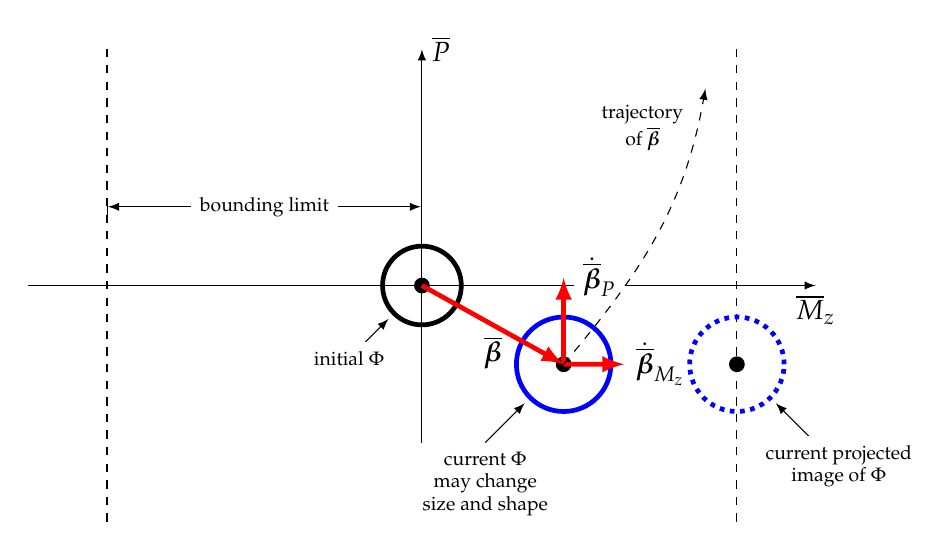
\begin{tikzpicture}[>=latex]
\draw[->](-5,0)--(5,0)node[below]{$\overline{M}_z$};
\draw[->](0,-3)--(0,3)node[right]{$\overline{P}$};
\coordinate(A)at(0,0);
\coordinate(B)at(1.8,-1);
\coordinate(C)at(4,-1);
\draw[|<->|](0,1)--++(180:4)node[midway,fill=white,font=\scriptsize]{bounding limit};
\node[fill=black,circle,inner sep=0,minimum size=2mm]at(A){};
\node[fill=black,circle,inner sep=0,minimum size=2mm]at(B){};
\node[fill=black,circle,inner sep=0,minimum size=2mm]at(C){};
\draw[dashed](-4,-3)--++(0,6);
\draw[dashed](4,-3)--++(0,6);
\node[circle,draw,line width=.6mm,minimum width=1cm,minimum height=1cm]at(A){};
\node[circle,draw=blue,line width=.6mm,minimum width=1.2cm,minimum height=1.2cm]at(B){};
\node[dotted,circle,draw=blue,line width=.6mm,minimum width=1.2cm,minimum height=1.2cm]at(C){};
\draw[->,draw=red,line width=.6mm](A)--(B)node[midway,below]{$\overline{\bbeta}$};
\draw[->,draw=red,line width=.6mm](B)--($(B)!.35!(C)$)node[right]{$\dot{\overline{\bbeta}}_{M_z}$};
\draw[->,draw=red,line width=.6mm](B)--++(0,1.1)node[right=1mm,fill=white]{$\dot{\overline{\bbeta}}_{P}$};
\draw[->,dashed](B)to[out=50,in=-100](3.6,2.5);
\draw[<-]($(B)+(-135:.7)$)--++(-.5,-.5)node[anchor=north,fill=white,align=center,font=\scriptsize]{current $\Phi$\\may change\\size and shape};
\draw[<-]($(A)+(-135:.6)$)--++(-.5,-.5)node[fill=white,align=center,font=\scriptsize]{initial $\Phi$};
\draw[<-]($(C)+(-45:.7)$)--++(.8,-.8)node[fill=white,align=center,font=\scriptsize]{current projected\\image of $\Phi$};
\node[align=center,font=\scriptsize]at(2.8,2){trajectory\\of $\overline{\bbeta}$};
\end{tikzpicture}
\end{document}